\documentclass[11pt,a4paper]{article}
\usepackage[utf8]{inputenc}
\usepackage[T1]{fontenc}
\usepackage[sc]{mathpazo}
\usepackage[scaled=0.92]{helvet}
\linespread{1.06}
\usepackage[a4paper,left=30mm,right=30mm,top=30mm,bottom=32mm,headsep=9mm,footskip=12mm]{geometry}
\usepackage{amsmath,amssymb,amsthm,mathtools}
\usepackage{microtype}
\usepackage{booktabs,array,longtable}
\usepackage{graphicx}
\usepackage{tikz}
\usetikzlibrary{arrows.meta,positioning,calc}
\usepackage{pgfplots}
\pgfplotsset{compat=1.17}
\usepackage{xcolor}
\usepackage{enumitem}
\usepackage{titlesec}
\usepackage{fancyhdr}
\usepackage[font=small,labelfont={sf,bf},labelsep=period,skip=6pt]{caption}
\definecolor{ink}{RGB}{24,48,82}
\definecolor{rulegray}{gray}{0.55}
\definecolor{inklight}{RGB}{226,233,243}
\definecolor{okgreen}{RGB}{46,110,78}
\definecolor{warnamber}{RGB}{176,112,20}
\definecolor{badred}{RGB}{160,52,44}
\usepackage[colorlinks=true,linkcolor=ink,citecolor=ink,urlcolor=ink,
  pdftitle={From Correlations to Geometry: A Conditional Spectral Reconstruction},
  pdfauthor={Michael Neuberger}]{hyperref}

% ---- headings ----
\titleformat{\section}{\sffamily\bfseries\large\color{ink}}{\thesection}{0.8em}{}
\titleformat{\subsection}{\sffamily\bfseries\normalsize}{\thesubsection}{0.8em}{}
\titleformat{\paragraph}[runin]{\sffamily\bfseries\small}{}{0pt}{}[.]
\titlespacing*{\section}{0pt}{2.4ex plus .6ex minus .2ex}{1.1ex plus .2ex}
\titlespacing*{\subsection}{0pt}{1.9ex plus .5ex minus .2ex}{0.8ex plus .2ex}
\titlespacing*{\paragraph}{0pt}{1.4ex plus .4ex minus .2ex}{0.6em}

% ---- running head ----
\pagestyle{fancy}
\fancyhf{}
\renewcommand{\headrulewidth}{0.3pt}
\renewcommand{\headrule}{{\color{rulegray}\hrule width\headwidth height\headrulewidth}}
\fancyhead[L]{\sffamily\footnotesize M.~Neuberger}
\fancyhead[R]{\sffamily\footnotesize From Correlations to Geometry\quad\textperiodcentered\quad v3}
\fancyfoot[C]{\sffamily\footnotesize\thepage}
\fancypagestyle{plain}{\fancyhf{}\renewcommand{\headrulewidth}{0pt}\fancyfoot[C]{\sffamily\footnotesize\thepage}}
\setlength{\headheight}{14pt}

% ---- theorems ----
\newtheoremstyle{stmt}{1.5ex plus .3ex}{1.5ex plus .3ex}{\itshape}{}{\sffamily\bfseries\small\color{ink}}{.}{0.6em}{}
\newtheoremstyle{defn}{1.5ex plus .3ex}{1.5ex plus .3ex}{\normalfont}{}{\sffamily\bfseries\small\color{ink}}{.}{0.6em}{}
\newtheoremstyle{rmk}{1.1ex plus .3ex}{1.1ex plus .3ex}{\normalfont}{}{\sffamily\itshape\small}{.}{0.6em}{}
\theoremstyle{stmt}
\newtheorem{theorem}{Theorem}[section]
\newtheorem{proposition}[theorem]{Proposition}
\newtheorem{lemma}[theorem]{Lemma}
\newtheorem{corollary}[theorem]{Corollary}
\theoremstyle{defn}
\newtheorem{assumption}[theorem]{Assumption}
\newtheorem{hypothesis}[theorem]{Hypothesis}
\newtheorem{definition}[theorem]{Definition}
\theoremstyle{rmk}
\newtheorem{remark}[theorem]{Remark}
\makeatletter
\renewenvironment{proof}[1][\proofname]{\par\pushQED{\qed}\normalfont\topsep6\p@\@plus6\p@\relax
  \trivlist\item[\hskip\labelsep{\sffamily\itshape\small #1.}]\ignorespaces}{\popQED\endtrivlist\@endpefalse}
\makeatother

% ---- lists ----
\setlist{itemsep=0.25ex,topsep=0.6ex,parsep=0.2ex}
\setlist[enumerate,1]{label=\textup{(\arabic*)},leftmargin=2.2em}
\setlist[itemize,1]{leftmargin=1.6em}

\numberwithin{equation}{section}
\setlength{\parskip}{0pt}
\setlength{\parindent}{1.2em}
\emergencystretch=1.5em

% ---- table of contents ----
\makeatletter
\renewcommand{\l@section}[2]{\addvspace{0.55ex}{\sffamily\small\bfseries\@dottedtocline{1}{0em}{1.8em}{#1}{#2}}}
\renewcommand{\l@subsection}[2]{{\sffamily\footnotesize\@dottedtocline{2}{1.8em}{2.6em}{#1}{#2}}}
\makeatother
\setcounter{tocdepth}{2}

% ---- figure styles ----
\tikzset{
  fbox/.style={draw=ink,line width=0.5pt,rounded corners=2pt,fill=inklight,font=\sffamily\footnotesize,align=center,inner sep=4pt},
  dbox/.style={draw=rulegray,line width=0.4pt,rounded corners=2pt,fill=white,font=\sffamily\footnotesize,align=left,inner sep=4pt},
  farr/.style={-{Stealth[length=5pt]},line width=0.6pt,draw=ink},
  fnote/.style={font=\sffamily\scriptsize,text=rulegray!60!black,align=center}}

\DeclareMathOperator{\Tr}{Tr}
\DeclareMathOperator{\tr}{tr}
\DeclareMathOperator{\Vol}{Vol}
\DeclareMathOperator{\Ric}{Ric}
\DeclareMathOperator{\Riem}{Riem}
\newcommand{\M}{\mathcal{M}}
\newcommand{\Lc}{\mathcal{L}}
\newcommand{\R}{\mathbb{R}}
\newcommand{\dd}{\mathrm{d}}
\newcommand{\Lcurv}{L_{\mathrm{curv}}}

\begin{document}
\thispagestyle{plain}

\noindent{\sffamily\bfseries\LARGE\color{ink} From Correlations to Geometry\par}
\vspace{4pt}
\noindent{\sffamily\Large A Conditional Spectral Reconstruction\par}
\vspace{10pt}
\noindent{\color{rulegray}\rule{\textwidth}{0.6pt}}\par
\vspace{8pt}
\noindent{\sffamily\normalsize Michael Neuberger}\par
\vspace{2pt}
\noindent{\small\textit{Versino PsiOmega GmbH}\quad\textperiodcentered\quad\texttt{neuberger@versino.de}\hfill Version~3\quad\textperiodcentered\quad 16 November 2026}\par
\noindent{\footnotesize\sffamily DOI: \href{https://doi.org/10.5281/zenodo.24273022}{10.5281/zenodo.24273022}\quad\textperiodcentered\quad all versions: \href{https://doi.org/10.5281/zenodo.16605659}{10.5281/zenodo.16605659}}\par
\vspace{16pt}

\noindent{\sffamily\bfseries\small Abstract}\par\vspace{3pt}
{\small\noindent We determine which parts of the programme ``geometry from correlations'' can be proven with present tools, and state the rest as assumptions or open problems. The input is a matrix $C_{ij}$ of correlations between local subsystems (mutual information) whose dependence on an underlying Riemannian distance is described by an isotropic profile; a density-normalised diffusion-map pipeline reconstructs the Laplace--Beltrami operator, its spectrum, a spectral embedding and the integrated curvature invariants. Much of this chain combines known mathematics. Three results are, to our knowledge, new. \emph{First}, the extrinsic curvature of the slice is stored in the time-odd part of the state: the symmetric part of the $\phi\pi$-correlator divided by the momentum correlator is the X-ray transform of $K$, also for non-stationary states, and no entropic quantity sees its sign. \emph{Second}, a cutoff carried by persistent nodes induces a gravitational action with a preferred foliation, of Ho\v{r}ava type. That fields which violate Lorentz invariance induce such an action is known; here the fields are Lorentz invariant and only the cutoff is tied to the slices. Its kinetic coupling satisfies $\lambda\le1$ for every node system whose Hamiltonian is linear in the shift, by concavity of the ground-state energy, whereas stability and observation require $\lambda\ge1$; we find $\lambda=-3$ for a minimally coupled scalar field, $\tfrac13$ for a Dirac field and $-\tfrac12$ for oscillators on the kernel graph, and the tensor modes do not propagate with the speed of the field. \emph{Third}, an exact Poisson representation of the graph heat trace shows that at a diffusion time comparable to the kernel scale the trace is dominated by a non-geometric term; after its subtraction the graph heat trace converges to that of the manifold.

\smallskip\noindent The reconstruction chain itself consists of: (i) the Laplace--Beltrami limit for radial profile kernels, independently of the sampling density; (ii) convergence of eigenvalues, with multiplicities and explicit rates, and of eigenvectors of simple eigenvalues, for every monotone profile and intrinsic distances, by a comparison of Dirichlet forms; (iii) an exact discrete isometry for the density-weighted spectral embedding; (iv) for Gaussian states of a massive scalar field the decay $r^{-D}e^{-2mr}$ of the mutual information of two modes, so that the surprisal distance is not asymptotically a metric but satisfies the profile assumption, its extension to curved backgrounds through the Van Vleck factor, and an end-to-end statement for the ground state of the free field on $\R\times\M$: the graph Laplacian built from the mutual informations of localised modes alone converges spectrally, with heat trace, if the correlation length and the mode size are small compared with the kernel scale; (v) a position-dependent gap is exactly a conformal factor of the metric or, for spatial correlations, the lapse of a static spacetime, and carries no dynamics of its own; (vi) for interacting systems the mutual information is the Gaussian value plus an explicit non-Gaussianity, and for finite-dimensional nodes it decays at exactly twice the rate of the correlations; (vii) for states of the vacuum type the Hamiltonian is contained in the state through the modular Hamiltonians of nested regions (cited theorems).

\smallskip\noindent Concerning dynamics, heat-trace functionals with a positive weight have no stationary metric, and Einstein metrics are the first-order fixed points of the normalised heat-kernel embedding. We do not derive the Einstein--Hilbert action or field equations: the geometry is recovered from data that already encode it. A coupling to matter requires an additional principle; two candidates, stationarity of the total effective action and entanglement equilibrium, lead to the same equation, both amount to treating the background as a summed-over variable, and a scalar response would give Nordstr\"om's theory instead. For special field contents (scalar fields coupled to the curvature, Maxwell and massive vector fields) the leading non-covariant terms of a node system cancel; for the fields we have computed, the cancellation of all non-covariant terms, including those of the vacuum energy, implies that the induced action itself vanishes through the order $m^2$. This last statement rests on explicit computation for the listed fields at second order around a flat slice, not on a structural proof, and is evidence rather than a no-go theorem. Neither principle is derived, and none of the proofs has been checked independently.\par}
\vspace{10pt}
\noindent{\color{rulegray}\rule{\textwidth}{0.3pt}}\par
\vspace{6pt}

\noindent{\footnotesize This is version~3 of the record. It supersedes version~2, ``Entropic Gravity via Quantum Causality, Part~I'' (18 August 2025, \href{https://doi.org/10.5281/zenodo.16895940}{doi:10.5281/zenodo.16895940}), and version~1 (30 July 2025, \href{https://doi.org/10.5281/zenodo.16605660}{doi:10.5281/zenodo.16605660}). Section~\ref{sec:changes} lists the changes with respect to version~2.\par}

\vspace{6pt}
{\makeatletter\renewcommand{\contentsname}{Contents}\makeatother
\begingroup\titleformat{\section}{\sffamily\bfseries\small}{}{0pt}{}\titlespacing*{\section}{0pt}{1ex}{0.6ex}
\tableofcontents\endgroup}
\vspace{4pt}
\noindent{\color{rulegray}\rule{\textwidth}{0.3pt}}\par



\section{Introduction}

The idea that spatial geometry is encoded in the entanglement structure of a quantum state has a substantial history \cite{Jacobson95,VanRaamsdonk,CCM}. Cao, Carroll and Michalakis \cite{CCM} define distances from the mutual information between factors of a Hilbert space and recover an approximate geometry by multidimensional scaling; a spatial analogue of Einstein's equation follows there from additional assumptions. The present paper asks a narrower question: given correlation data of this type, \emph{which reconstruction statements are theorems?}

\paragraph{Related work} That a metric is encoded in the two-point functions of quantum fields is known in a different form. Saravani, Aslanbeigi and Kempf \cite{SAK} express the metric of a curved spacetime through the Feynman propagator of a scalar field, Kempf \cite{Kempf21} proposes correlators as a replacement for the notion of distance, and Perche and Mart\'in-Mart\'inez \cite{PercheMM} obtain the metric from the Wightman function for general field states and describe its measurement with local probes. These constructions are local: they use the short-distance behaviour of the correlator of a known field on a given spacetime. The present paper uses the long-distance decay of an entropic quantity between subsystems on a slice, which does not presuppose which observable is the field, and asks for convergence statements for a finite sample of nodes. The two approaches meet where causal cones and the lapse enter (Sections~\ref{sec:scalar} and~\ref{sec:time}). On the side of dynamics, it is known that integrating out fields that violate Lorentz invariance induces a gravitational action of Ho\v{r}ava--Lifshitz type \cite{NS10,DSS,LMP}; the relation to Section~\ref{sec:matter} is discussed in Section~\ref{sec:nodecov}.

Our pipeline is that of diffusion maps \cite{CoifmanLafon}:
\begin{equation}\label{eq:pipeline}
C \;\longrightarrow\; (V,W) \;\longrightarrow\; \Lc \;\longrightarrow\; H_t=e^{-t\Lc} \;\longrightarrow\; \text{embedding and heat trace}.
\end{equation}
Figure~\ref{fig:sketch} illustrates the idea and Figure~\ref{fig:pipeline} shows the chain together with the results that control each step.

\begin{figure}[t]
\centering
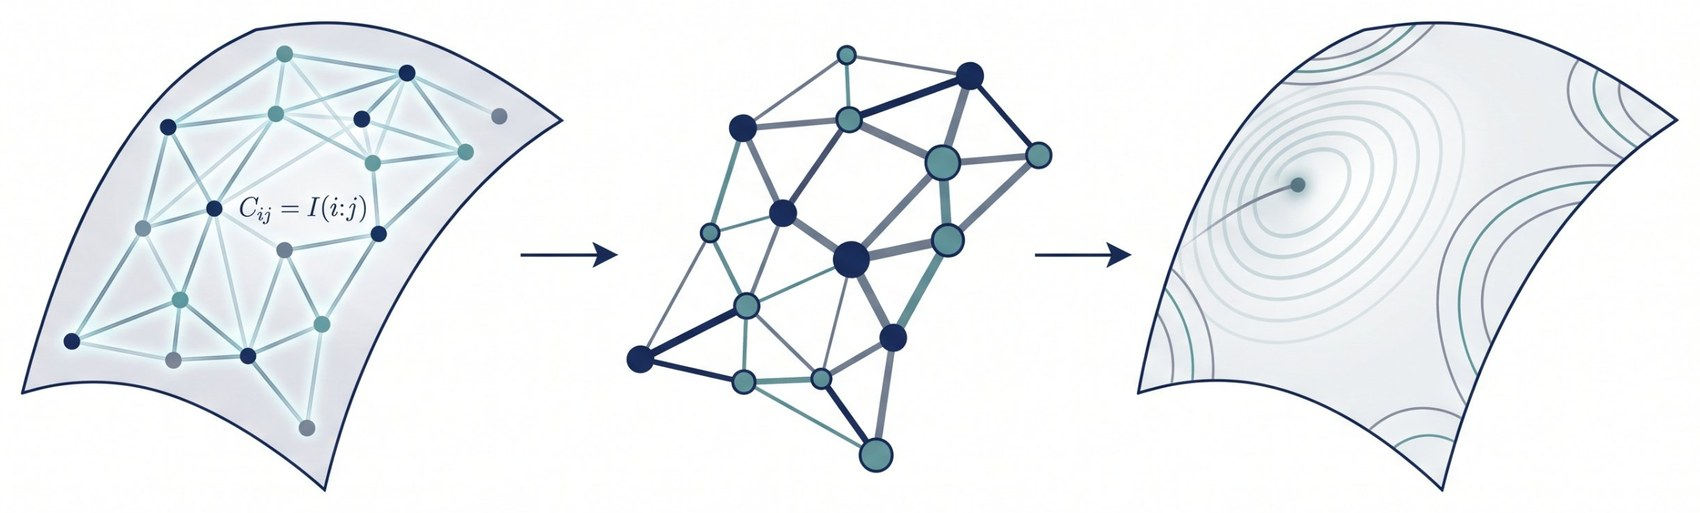
\includegraphics[width=0.9\textwidth]{figures/fig_pipeline_sketch.jpg}
\caption{The reconstruction in pictures: subsystems on a slice with their pairwise mutual informations $C_{ij}$; the weighted graph built from them; the geometry recovered through the heat kernel of the graph Laplacian. Schematic. The schematic illustrations of this paper (this figure and Figures~\ref{fig:scales}, \ref{fig:heatsketch}, \ref{fig:modes}, \ref{fig:lapse}, \ref{fig:xray}, \ref{fig:modular}, \ref{fig:nordstrom}, \ref{fig:foliation} and~\ref{fig:sphere}) were produced with a generative image model from the text and are not drawn to scale or from data.}\label{fig:sketch}
\end{figure}


\begin{figure}[t]
\centering
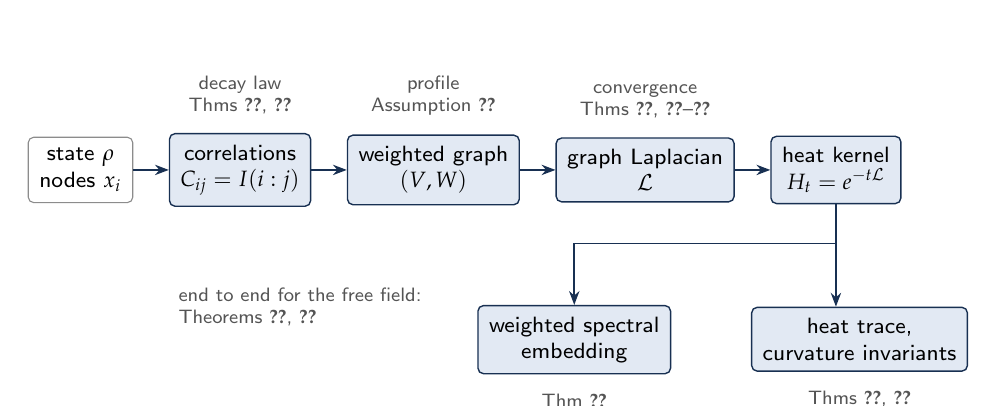
\begin{tikzpicture}[node distance=4.5mm]
\node[dbox,align=center] (state) {state $\rho$\\nodes $x_i$};
\node[fbox,right=of state] (C) {correlations\\$C_{ij}=I(i:j)$};
\node[fbox,right=of C] (W) {weighted graph\\$(V,W)$};
\node[fbox,right=of W] (L) {graph Laplacian\\$\Lc$};
\node[fbox,right=of L] (H) {heat kernel\\$H_t=e^{-t\Lc}$};
\node[fbox,below=13mm of L,xshift=-9mm] (emb) {weighted spectral\\embedding};
\node[fbox,below=13mm of H,xshift=3mm] (tr) {heat trace,\\curvature invariants};
\draw[farr] (state)--(C); \draw[farr] (C)--(W); \draw[farr] (W)--(L); \draw[farr] (L)--(H);
\draw[farr] (H.south)--(H.south|-tr.north);
\draw[farr] (H.south)++(0,-5mm)-|(emb.north);
\node[fnote,above=1.2mm of C] {decay law\\Thms~\ref{thm:decay}, \ref{thm:curved}};
\node[fnote,above=1.2mm of W] {profile\\Assumption~\ref{ass:profile}};
\node[fnote,above=1.2mm of L] {convergence\\Thms~\ref{thm:LB}, \ref{thm:eig}--\ref{thm:rate2}};
\node[fnote,below=1.2mm of tr] {Thms~\ref{thm:poisson}, \ref{thm:trace}};
\node[fnote,below=1.2mm of emb] {Thm~\ref{thm:isometry}};
\node[fnote,anchor=north west,align=left] at ($(C.south west)+(0,-9mm)$) {end to end for the free field:\\Theorems~\ref{thm:window}, \ref{thm:e2e}};
\end{tikzpicture}
\caption{The reconstruction pipeline \eqref{eq:pipeline} and the results that control each step. The input is the matrix of mutual informations alone; the background geometry enters only through the profile assumption.}\label{fig:pipeline}
\end{figure}

Three of the four ingredients are known mathematics: the density-normalised graph Laplacian \cite{CoifmanLafon,BelkinNiyogi,HAvL,THJ,ChengWu,BIK,GTGHS}, the heat-kernel embedding of B\'erard, Besson and Gallot \cite{BBG}, and the heat-trace expansion \cite{Gilkey}. Using the heat trace as a gravitational action is the spectral action principle of Chamseddine and Connes \cite{CC97} applied to the scalar Laplacian, and is closely related to Sakharov's induced gravity \cite{Sakharov,Visser}. Pointwise limits of graph Laplacians for kernel shapes other than the Gaussian are also known \cite{HAvL,THJ}; Theorem~\ref{thm:LB} is a statement of this kind, and what is specific to it is the formulation in the intrinsic distance with the density normalisation. What we add is listed below. The items that we believe to be new in substance, rather than a combination or sharpening of known results, are the Poisson representation of the heat trace (item~4), the description of the time-odd part of the state (item~7), and the analysis of the action induced by a node system in Sections~\ref{sec:nodecov}--\ref{sec:graphfields}, which is not part of the reconstruction and is summarised in Section~\ref{sec:nodesummary}.

\begin{enumerate}
\item A formulation of the geometric input as an \emph{isotropic profile} (Assumption~\ref{ass:profile}) rather than as an approximate isometry, and a proof that the Laplace--Beltrami limit holds for every such profile (Theorem~\ref{thm:LB}). This matters because the approximate-isometry form fails already for free fields in flat space (Corollary~\ref{cor:drift}).
\item Spectral convergence for monotone profiles and intrinsic distances: eigenvalues with multiplicities and rates (Theorem~\ref{thm:eig}), eigenvectors and eigenspaces (Theorems~\ref{thm:evec}, \ref{thm:cluster}), and stability under perturbations of the kernel (Proposition~\ref{prop:stab}). The proof compares Dirichlet forms and uses no property of the Gaussian kernel.
\item A density-weighted spectral embedding with an exact discrete isometry (Theorem~\ref{thm:isometry}); without the weight the embedding depends on the sampling density.
\item An exact Poisson representation of the graph heat trace (Theorem~\ref{thm:poisson}). It shows that the trace at diffusion time $t\sim\xi^2$, with $\xi$ the kernel scale, is not a geometric quantity. After subtraction of the explicit term $Ne^{-\tau}$ the graph heat trace converges to the heat trace of the manifold (Theorem~\ref{thm:trace}).
\item The decay law of mutual information for Gaussian states (Theorem~\ref{thm:decay}), which replaces an incorrect argument via the Bisognano--Wichmann theorem in the earlier manuscript, its extension to curved backgrounds (Theorem~\ref{thm:curved}), and an end-to-end statement: for the ground state of the free field on $\R\times\M$, with one localised mode per node, the pipeline built from the mutual informations alone converges spectrally to the Laplace--Beltrami operator (Theorems~\ref{thm:window}, \ref{thm:e2e}).
\item An exact description of a position-dependent gap (Section~\ref{sec:scalar}): it is a conformal factor (Proposition~\ref{prop:weyl}) or a lapse function (Proposition~\ref{prop:lapse}), the correlators have explicit asymptotics in which the lapse appears as a Van Vleck factor in the time direction (Theorem~\ref{thm:vargap}), and it carries no dynamics of its own (Proposition~\ref{prop:conformal}).
\item The time-odd part of the state: an exact kinematic identity, the extrinsic curvature as an X-ray transform of the $\phi\pi$-correlator (Proposition~\ref{prop:kin}, Theorems~\ref{thm:xray}, \ref{thm:YP}), a graph estimator (Proposition~\ref{prop:Kgraph}), and the fact that no entropic quantity sees the sign of $K$ (Proposition~\ref{prop:Todd}).
\item For interacting systems, an exact decomposition of the mutual information into its Gaussian value and a non-Gaussianity (Proposition~\ref{prop:nonG}), and for the coupling to matter a comparison of two principles (Proposition~\ref{prop:principles}).
\item Two statements about dynamics: no heat-trace functional with positive weight has a stationary metric (Theorem~\ref{thm:nostat}), and Einstein metrics are the first-order fixed points of the normalised heat-kernel embedding (Corollary~\ref{cor:fixed}).
\end{enumerate}

\paragraph{What is not claimed} The construction is \emph{background-recovering}: Assumption~\ref{ass:profile} refers to a Riemannian manifold. We do not obtain geometry from a geometry-free starting point. The reconstructed manifold is Riemannian; if $C_{ij}$ is the mutual information of local algebras in a state, it is a \emph{spatial} manifold, and the heat-trace expansion yields a functional of the spatial geometry, not the four-dimensional Einstein--Hilbert action (Section~\ref{sec:reading}). No field equation is derived.

\paragraph{Overview} Figure~\ref{fig:blocks} summarises which ingredients of a spacetime are found in which part of the data, and with what status.

\begin{figure}[t]
\centering
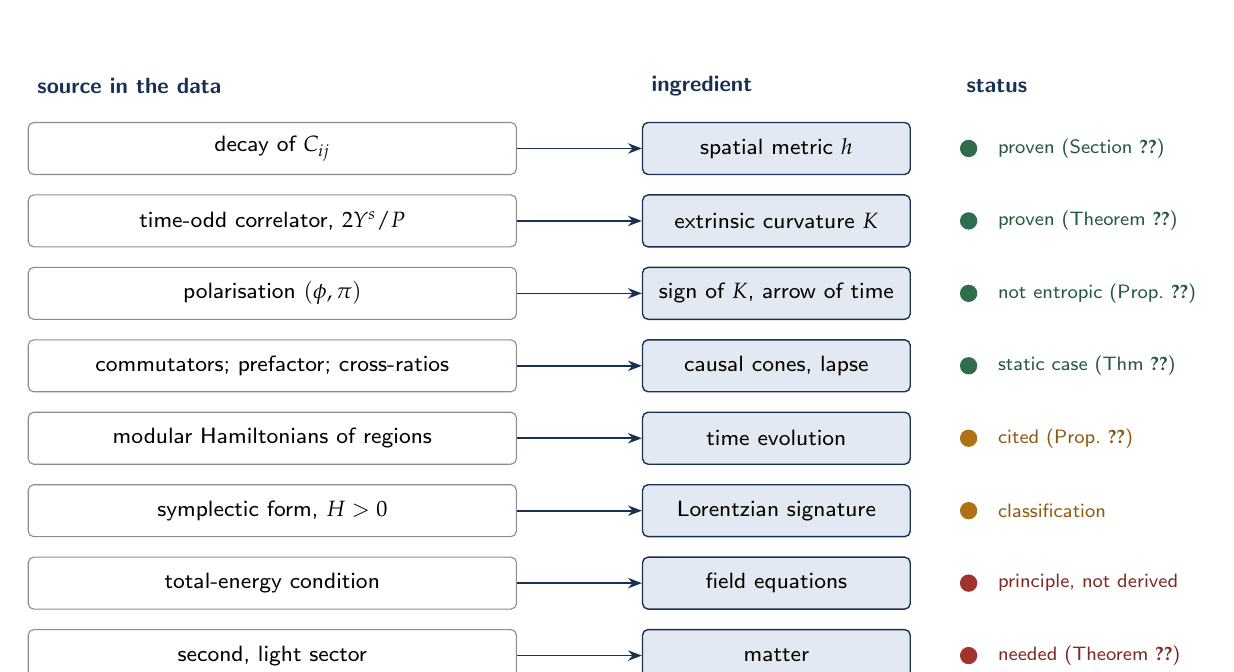
\begin{tikzpicture}[x=1mm,y=1mm]
\def\rowh{9.2}
\node[font=\sffamily\footnotesize\bfseries,text=ink,anchor=west] at (0,5) {source in the data};
\node[font=\sffamily\footnotesize\bfseries,text=ink,anchor=west] at (78,5) {ingredient};
\node[font=\sffamily\footnotesize\bfseries,text=ink,anchor=west] at (118,5) {status};
\foreach \i/\src/\ing/\col/\st in {
 0/{decay of $C_{ij}$}/{spatial metric $h$}/okgreen/{proven (Section~\ref{sec:recon})},
 1/{time-odd correlator, $2Y^s/P$}/{extrinsic curvature $K$}/okgreen/{proven (Theorem~\ref{thm:xray})},
 2/{polarisation $(\phi,\pi)$}/{sign of $K$, arrow of time}/okgreen/{not entropic (Prop.~\ref{prop:Todd})},
 3/{commutators; prefactor; cross-ratios}/{causal cones, lapse}/okgreen/{static case (Thm~\ref{thm:vargap})},
 4/{modular Hamiltonians of regions}/{time evolution}/warnamber/{cited (Prop.~\ref{prop:modular})},
 5/{symplectic form, $H>0$}/{Lorentzian signature}/warnamber/{classification},
 6/{total-energy condition}/{field equations}/badred/{principle, not derived},
 7/{second, light sector}/{matter}/badred/{needed (Theorem~\ref{thm:nostat})}}
{
 \pgfmathsetmacro{\y}{-\i*\rowh-3}
 \node[dbox,minimum width=62mm,minimum height=6.6mm,anchor=west] (s\i) at (0,\y) {\src};
 \node[fbox,minimum width=34mm,minimum height=6.6mm,anchor=west,align=left] (g\i) at (78,\y) {\ing};
 \draw[farr] (s\i.east)--(g\i.west);
 \fill[\col] (119.5,\y) circle (1.1);
 \node[font=\sffamily\scriptsize,anchor=west,text=\col!80!black] at (122,\y) {\st};
}
\end{tikzpicture}
\caption{Ingredients of a spacetime and where they are found in the data of a quantum state. Green: proven in this paper; amber: cited theorems or classification; red: requires an input that is not derived (Section~\ref{sec:central}). The scalar degree of freedom of Section~\ref{sec:scalar} is not a separate ingredient: it is the lapse or a conformal factor.}\label{fig:blocks}
\end{figure}

\paragraph{Status of the statements} Table~\ref{tab:status} lists every numbered result with its status. ``Proven'' means that a complete proof is given in this paper; none of the proofs has been checked by an independent reader.

{\small\setlength{\LTpre}{8pt}\setlength{\LTpost}{8pt}
\begin{longtable}{@{}>{\raggedright\arraybackslash}p{0.19\textwidth}>{\raggedright\arraybackslash}p{0.34\textwidth}>{\raggedright\arraybackslash}p{0.39\textwidth}@{}}
\caption{Results and their status.}\label{tab:status}\\
\toprule
\sffamily\bfseries Result & \sffamily\bfseries Statement & \sffamily\bfseries Status\\
\midrule
\endfirsthead
\multicolumn{3}{@{}l}{\sffamily\footnotesize Table~\thetable\ (continued)}\\
\toprule
\sffamily\bfseries Result & \sffamily\bfseries Statement & \sffamily\bfseries Status\\
\midrule
\endhead
\midrule
\multicolumn{3}{r@{}}{\sffamily\footnotesize continued on the next page}\\
\endfoot
\bottomrule
\endlastfoot
Theorem~\ref{thm:LB} & Laplace--Beltrami limit for profile kernels & proven\\
Theorems~\ref{thm:eig}--\ref{thm:rate2} & convergence of eigenvalues, eigenvectors and eigenspaces & proven; the random input is the transport estimate of \cite{GTS,GTGHS} (Lemma~\ref{lem:transport})\\
Proposition~\ref{prop:stab} & stability under kernel perturbations & proven\\
Theorem~\ref{thm:isometry} & exact weighted isometry & proven\\
Proposition~\ref{prop:BBG} & metric expansion of the embedding & cited from \cite{BBG}\\
Theorem~\ref{thm:poisson} & Poisson representation of the heat trace & proven; the identity machine-checked for real symmetric matrices, the bounds in coefficientwise and spectral form (Remark~\ref{rem:lean})\\
Theorem~\ref{thm:trace} & convergence of the subtracted heat trace & proven; the deterministic part of the proof machine-checked for real symmetric matrices, the eigenvalue estimates and the limit not (Remark~\ref{rem:lean})\\
Propositions~\ref{prop:moments}, \ref{prop:heatbounds} & return moments; refined bounds for the heat trace & proven; partly machine-checked (Remark~\ref{rem:lean})\\
Corollary~\ref{cor:subtractions} & independence of the subtraction and of the self-loops & proven, using Lemmas~\ref{lem:weights}, \ref{lem:traces}\\
Theorem~\ref{thm:rate} & rate $\xi^2/t$ of the subtracted trace, exactly solvable case & proven; estimates for the modes and the Poisson identity machine-checked, given the existence of the sums over the modes (Remark~\ref{rem:lean})\\
Proposition~\ref{prop:ratereduction} & rate $\xi^2/t$ for the sampled graph & conditional on the hypothesis \eqref{eq:eigrate2}\\
Proposition~\ref{prop:discrete} & heat trace from $\Tr P^k$, without subtraction & proven under a lower bound on the spectrum of $S$\\
Theorem~\ref{thm:corrected} & corrected estimator $T_\sigma-\tfrac{\sigma t}2T_\sigma''$, relative error $O(\tau^{-2})$ & proven; estimates for single modes, low and high, machine-checked\\
Theorem~\ref{thm:profile} & profiles other than Gaussian: coefficients $\beta$ and $\beta-1$ & proven at the population level, under (F1)--(F3); hypothesis (F2) completed after a counterexample to the earlier wording; estimates for single modes machine-checked\\
Theorem~\ref{thm:fixedxi}, Corollary~\ref{cor:torus} & limit $N\to\infty$ at fixed $\xi$; sharpness of $\xi^2/t$ for the sampled graph on a flat torus & proven, using the strong law for $U$-statistics \cite{Serfling}; the series step machine-checked, the laws of large numbers not\\
Proposition~\ref{prop:rateN} & rate $\sqrt{\log N/N}$ at fixed $\xi$ & proven, using \cite{Hoeffding}; not uniform in $\xi$\\
Proposition~\ref{prop:oracle} & fluctuations of order $1/N$ on a torus & proven for the exact normalisation, using \cite{Serfling}\\
Theorem~\ref{thm:profileHS} & profiles with a jump (indicator of a ball: $\beta=\tfrac{d+2}{d+4}$) & proven at the population level\\
Proposition~\ref{prop:estimated} & error $\log N/N$ in probability on a torus, estimated normalisation & proven, using \cite{Hoeffding,Serfling}\\
Theorem~\ref{thm:jointslow} & rate $\xi^2/t$ for the sampled graph in a joint regime, $\xi_N^{d+2}\log N\ge64$ & proven; constants tracked in the proof of Proposition~\ref{prop:rateN}\\
Lemma~\ref{lem:oraclemoments}, Theorem~\ref{thm:jointpoly} & rate $\xi^2/t$, with the sharp coefficient, for the sampled graph on a flat torus when $N\xi_N^{2d+6}/\log N\to\infty$ & proven (in probability); elementary inequalities machine-checked\\
Proposition~\ref{prop:bias} & bias of $\Tr P^k$ of the order $1/N$ on a flat torus, with and without self-loops, with its coefficient & proven for fixed $\xi$ and $k$; numerics\\
Proposition~\ref{prop:variance} & variance of $\Tr P^k$ of the order $1/N^2$ on a flat torus, with its coefficient & proven for fixed $\xi$ and $k$; numerics\\
Lemmas~\ref{lem:pgauss}, \ref{lem:consistency}, Theorem~\ref{thm:kernel}, Corollaries~\ref{cor:kernel-trace}, \ref{cor:kernel-corrected}, \ref{cor:kernel-noloops} & kernel of the sampled walk on a flat torus within $C\sqrt{kM\log N/N}\,m_k$ of the heat kernel, uniformly in $k$; convergence of the trace for $N\xi_N^{d+2}/\log N\to\infty$ and the rate $\xi^2/t$ with the sharp coefficient for $N\xi_N^{d+6}/\log N\to\infty$, almost surely; the corrected estimator on the sampled graph; the graph without self-loops & proven; written and read by two sessions of an AI system only; the estimate of Theorem~\ref{thm:kernel} is machine-checked with an explicit, much larger constant and an exceptional event of its own (Remark~\ref{rem:lean}), the corollaries are not; numerics\\
Proposition~\ref{prop:reduction}, Lemmas~\ref{lem:degenerate}, \ref{lem:pibound}, Corollary~\ref{cor:secondstage} & rate $\xi^2/t$ with the sharp coefficient on a flat torus of dimension at most two when $N\xi_N^{d+4}/\log N\to\infty$ (dimension three: $N\xi_N^7/(\log N)^2\to\infty$), in probability & proven; written by one session of an AI system and read once by a further session of the same system, by no person; numerics\\
Lemma~\ref{lem:kernelmatrix}, Theorem~\ref{thm:eigtorus}, Corollaries~\ref{cor:eigspace}, \ref{cor:deloc} & eigenvalues of the sampled graph on a flat torus, uniformly in the index and with multiplicities: within $C(\log N/N\xi^{d+2})^{1/2}\lambda_k^{(d+1)/2}$ of the eigenvalues of the population walk; \eqref{eq:eigrate2} for $N\xi_N^{3d}/\log N\to\infty$; eigenspaces in the Euclidean norm; delocalisation of the eigenvectors & proven; written by one session of an AI system and read once by a further session of the same system, by no person; the first inequality of part (ii) of Theorem~\ref{thm:eigtorus} for the nonzero eigenvalues is machine-checked with an explicit, much larger constant and an exceptional event of its own (Remark~\ref{rem:lean}), part (i) and the corollaries are not; numerics\\
Lemma~\ref{lem:kernel-l1}, Proposition~\ref{prop:reduction-alld}, Corollary~\ref{cor:secondstage-alld}, Theorem~\ref{thm:eigtorus-l1} & the kernel of the sampled walk in the mean over one index, $\frac1N\sum_a|N(P^k)_{ai}-p_k(x_a-x_i)|\le C\delta'\sqrt k$, from a stationary weight; with it the rate $\xi^2/t$ with the sharp coefficient in probability for $N\xi_N^{d+4}/\log N\to\infty$ in every dimension, and eigenvalues within $C\frac{\delta'}\xi\lambda_k^{1/2}+C\sqrt{\log N/N}\,\lambda_k^{(d+2)/2}$ of those of the population walk, which gives \eqref{eq:eigrate2} for $N\xi_N^{\max(d+2,2d)}/\log N\to\infty$ & proven; written by a second session of an AI system and read line by line by the author-side session, by no person; a form of the lemma is machine-checked, the other three statements are not; numerics\\
Remarks~\ref{rem:bias}(v), \ref{rem:variance}(v) & relative bias a bounded multiple of $M/N$ and relative fluctuation of the order $\sqrt M/N$, uniformly in $k$; rate $\xi^2/t$ for $N\xi_N^{d+2}\to\infty$ & conjecture; numerics\\
Proposition~\ref{prop:fixedxijump} & limit $N\to\infty$ for profiles with jumps & proven, using \cite{vdVW}\\
Propositions~\ref{prop:sphere}, \ref{prop:spheregap}, Corollary~\ref{cor:sphere} & round sphere: heat trace at the rescaled time $\sigma(1-\xi^2/6)$ & proven for small $\xi$, using \cite{Szego}; numerics\\
Remark~\ref{rem:rateopen} & sharp rate in the joint regime for $\xi_N$ below $(\log N/N)^{1/(d+4)}$ (dimension at most two); manifolds other than the flat torus in the joint regime; \eqref{eq:eigrate2} & open\\
Corollary~\ref{cor:curv} & curvature invariants & follows from \cite{Gilkey}\\
Propositions~\ref{prop:classical}, \ref{prop:twomode} & mutual information of Gaussian variables and of two modes & proven\\
Theorem~\ref{thm:decay} & decay law $r^{-D}e^{-2mr}$ & proven in flat space, one mode per node\\
Theorem~\ref{thm:curved} & correlators on a curved background & proven, using the heat-kernel asymptotics of \cite{Ludewig}\\
Proposition~\ref{prop:modes}, Corollary~\ref{cor:curvedMI} & geodesic modes and their mutual information on a curved background & proven, using \cite{Ludewig}\\
Proposition~\ref{prop:window}, Theorem~\ref{thm:window} & reconstruction from data that are near-isometric on a window & (i) proven; (ii), (iii) by re-running earlier proofs, not rewritten line by line\\
Theorem~\ref{thm:e2e} & end-to-end reconstruction for the free field on $\R\times\M$ & proven, given Theorem~\ref{thm:window} and the heat-kernel bound of \cite{LY}\\
Propositions~\ref{prop:weyl}--\ref{prop:conformal} & position-dependent gap & proven (exact identities)\\
Theorem~\ref{thm:vargap}, Proposition~\ref{prop:crossratio} & correlators $X$, $P$ for a variable gap; lapse from cross-ratios & proven, using \cite{Ludewig}; the latter at leading order, $D=1$\\
Proposition~\ref{prop:rigid} & rigidity of the lapse reconstruction, $D\ge2$ & proven (necessary condition)\\
Proposition~\ref{prop:kin}, Theorems~\ref{thm:xray}, \ref{thm:YP}, Proposition~\ref{prop:Todd} & time-odd correlator and extrinsic curvature & proven: exact identity; X-ray form exact on flat slices to first order in the shift, and in general wherever the correlator is a profile of the distance\\
Propositions~\ref{prop:Kgraph}, \ref{prop:dotL} & graph estimator for $K$; differentiated pipeline & proven; the latter at the population level\\
Proposition~\ref{prop:multimode} & several modes per node & proven (constants not explicit)\\
Proposition~\ref{prop:nonG}, Corollary~\ref{cor:firstorder} & interacting systems & exact identity; first-order statement under a regularity hypothesis\\
Theorem~\ref{thm:cluster2}, Corollary~\ref{cor:gapped} & two-sided bound, finite-dimensional nodes & proven; gapped lattice systems via \cite{HastingsKoma}\\
Proposition~\ref{prop:modular} & time from modular data & cited theorems; lattice form verified numerically\\
Proposition~\ref{prop:vacuum} & vacuum term and field content & proven (one-loop heat-kernel computation)\\
Proposition~\ref{prop:nordstrom}, Section~\ref{sec:central} & scalar response; forms of the missing input & proven; (P1) reduced to a stated hypothesis, not derived\\
Propositions~\ref{prop:shiftresponse}, \ref{prop:nocancel} & non-covariant shift response of node systems; no cancellation by field content if the Hamiltonian is linear in the shift & proven (second order in the shift; leading order in derivatives)\\
Proposition~\ref{prop:lambda} & kinetic coupling $\lambda\le1$ of node systems & proven for the kinetic sector on flat slices; comparison with stability and observation uses cited results\\
Proposition~\ref{prop:relations}, Corollary~\ref{cor:vanish} & linear relations between kinetic, longitudinal, curvature and vacuum terms; covariance and vanishing vacuum energy imply a vanishing induced action & verified on scalar, Dirac, Maxwell and massive vector fields; at leading order confirmed on form fields in all dimensions $D\le12$ and derived for them (Proposition~\ref{prop:pforms}, Remark~\ref{rem:reduced}); no derivation covering fermions and the finite parts\\
Propositions~\ref{prop:massterms}, \ref{prop:profile}, Corollary~\ref{cor:nextorder} & terms of order $m^2\ln\Lambda$ (covariant) and $m^2$ (not covariant); independence of the cutoff profile; $\lambda<1$ at this order without massive vector fields, tuned solutions with them & proven for scalar, Dirac and vector fields and for monotone mode-weight profiles; not for lattice or graph dispersions\\
Propositions~\ref{prop:nonmin}, \ref{prop:maxwell}, Corollary~\ref{cor:content} & non-minimally coupled scalar field, Maxwell field; field contents for which the leading non-covariant terms cancel & proven at second order on flat slices, leading order in the cutoff; curvature terms formal for sharp cutoffs\\
Propositions~\ref{prop:dirac}, \ref{prop:graphlong} & Dirac field ($\lambda=1/D$); oscillators on the kernel graph ($\lambda=-\tfrac12$) & proven at second order on flat slices; the graph statement at the population level, sampling corrections checked numerically only\\
Propositions~\ref{prop:lapseresponse}--\ref{prop:curvterm} & lapse, tensor kinetic term and curvature term of node systems; tensor speed & proven at second order on flat slices and at the population level; heat-kernel expansion used formally for sharp cutoffs; preferred-frame parameters via formulas cited from \cite{GSS}\\
Proposition~\ref{prop:principles} & coupling to matter & conditional on a principle; combines cited results\\
Theorem~\ref{thm:nostat} & no stationary metric & proven\\
Corollary~\ref{cor:fixed} & Einstein metrics as fixed points & follows from \cite{BBG}\\
\end{longtable}}

\section{Setting and construction}\label{sec:setting}

\subsection{Correlation data}

Let $V=\{1,\dots,N\}$ index a family of subsystems of a quantum system in a state $\rho$, and let
\begin{equation}
C_{ij}=I(i:j)=S(\rho_i)+S(\rho_j)-S(\rho_{ij}),\qquad i\ne j,
\end{equation}
be their mutual information. For a lattice system the subsystems are finite-dimensional and all entropies are finite; in Section~\ref{sec:gauss} each subsystem is a single bosonic mode. Fix constants $C_0,\xi_0>0$ and a scale $\xi>0$ and define, as in \cite{CCM}, the surprisal distance and the bare affinity
\begin{equation}\label{eq:surprisal}
d_C(i,j)=-\xi_0\ln\min\{C_{ij}/C_0,1\},\qquad K_{ij}=\exp\!\Big(-\frac{d_C(i,j)^2}{2\xi^2}\Big),\qquad K_{ii}=1 .
\end{equation}
In general $d_C$ is not a metric.

\begin{assumption}[Isotropic profile]\label{ass:profile}
There exist a closed connected smooth Riemannian manifold $(\M,g)$ of dimension $d$, points $x_1,\dots,x_N\in\M$ drawn independently from a probability density $\mu\in C^6(\M)$, $\mu>0$, with respect to $\dd V_g$, and a nonincreasing function $h:[0,\infty)\to[0,\infty)$, not identically zero on $(0,\infty)$, with $h(s)\le A e^{-s}$, such that
\begin{equation}\label{eq:profile}
K_{ij}=h\big(d_g(x_i,x_j)/\xi\big)\qquad (i\ne j).
\end{equation}
\end{assumption}

The assumption holds whenever $C_{ij}=F(d_g(x_i,x_j))$ with one nonincreasing function $F$ for all pairs; then $h(s)=\exp(-\psi(\xi s)^2/2\xi^2)$ with $\psi=-\xi_0\ln\min\{F/C_0,1\}$, which is nonincreasing. The profile is fixed if the scales of $F$ are held in fixed ratio to $\xi$. What the assumption demands physically is that the correlation profile is the same at every point and in every direction. Monotonicity of $h$ is not needed for Theorem~\ref{thm:LB}, which holds for bounded measurable profiles; it is used in Section~\ref{sec:spec}. Perturbations of \eqref{eq:profile} are treated in Remark~\ref{rem:robust} and Proposition~\ref{prop:stab}.

We write
\begin{equation}
m_0=\int_{\R^d}h(|u|)\,\dd u,\qquad m_2=\int_{\R^d}h(|u|)\,u_1^2\,\dd u,\qquad c_h=\frac{m_2}{m_0}.
\end{equation}
For the Gaussian profile $h(s)=e^{-s^2/2}$ one has $c_h=1$.

\subsection{Graph operators}

Following Coifman and Lafon \cite{CoifmanLafon} we remove the sampling density by a two-sided normalisation:
\begin{equation}\label{eq:W}
q_i=\frac1N\sum_k K_{ik},\qquad W_{ij}=\frac{K_{ij}}{q_iq_j},\qquad D_i=\sum_jW_{ij},\qquad \pi_i=\frac{D_i}{\sum_kD_k}.
\end{equation}
Let $D=\operatorname{diag}(D_i)$, $P=D^{-1}W$ (row-stochastic) and $S=D^{-1/2}WD^{-1/2}$ (symmetric). The graph Laplacian and its heat semigroup are
\begin{equation}\label{eq:L}
\Lc=\frac{2}{c_h\xi^2}\,(I-S),\qquad H_t=e^{-t\Lc},\qquad \tau\equiv\frac{2t}{c_h\xi^2}.
\end{equation}
We denote by $0=\lambda_0^{N}\le\lambda_1^{N}\le\dots$ the eigenvalues of $\Lc$ and by $v_a$ an orthonormal eigenbasis, and by $0=\lambda_0<\lambda_1\le\dots$ and $\psi_a$ the eigenvalues and $L^2(\dd V_g)$-orthonormal eigenfunctions of $-\Delta_g$.

\section{Reconstruction theorems}\label{sec:recon}

\subsection{The Laplace--Beltrami limit}

The population versions of \eqref{eq:W} are, with $K_\xi(x,y)=h(d_g(x,y)/\xi)$,
\begin{equation}
\begin{gathered}
q_\xi(x)=\int K_\xi(x,y)\mu(y)\,\dd V(y),\qquad
W_\xi(x,y)=\frac{K_\xi(x,y)}{q_\xi(x)q_\xi(y)},\\
(P_\xi f)(x)=\frac{\int W_\xi(x,y)f(y)\mu(y)\,\dd V(y)}{\int W_\xi(x,y)\mu(y)\,\dd V(y)} .
\end{gathered}
\end{equation}

\begin{theorem}[Laplace--Beltrami limit for profile kernels]\label{thm:LB}
Under Assumption~\ref{ass:profile}, for every $f\in C^6(\M)$,
\begin{equation}
\frac{2}{c_h\xi^2}\,\big(f-P_\xi f\big)=-\Delta_gf+O(\xi^2)
\end{equation}
uniformly on $\M$. The limit does not depend on $\mu$.
\end{theorem}

The proof is in Appendix~\ref{app:LB}. For the Gaussian profile this is the result of \cite{CoifmanLafon}. The passage from $P_\xi$ to the $N$-point operator $P$ at the level of the spectrum is the subject of Section~\ref{sec:spec}.

\begin{remark}[Robustness]\label{rem:robust}
The proof shows that every contribution of the form $\xi^2\cdot(\text{function})\cdot f$ cancels between numerator and denominator of $P_\xi f$. This is why the density $\mu$, the scalar curvature, and any relative correction $1+\xi^2\omega(x)$ to the kernel drop out.
\end{remark}

\subsection{Spectral convergence}\label{sec:spec}

Pointwise convergence of the generator does not control the spectrum. For the Gaussian kernel with Euclidean distances, convergence of eigenvalues and eigenvectors with rates was proven by Cheng and Wu \cite{ChengWu}; for compactly supported kernels see \cite{BIK,GTGHS}, and for the flat torus \cite{WormellReich}. None of these results covers a general profile $h$ with intrinsic distances, which is the case needed here (Corollary~\ref{cor:drift}). We therefore prove spectral convergence directly, by the comparison of Dirichlet forms that Burago, Ivanov and Kurylev \cite{BIK} introduced for $\varepsilon$-nets and that was combined with optimal transport in \cite{GTGHS}. The variational form suits the present operator: by \eqref{eq:L} the $\lambda_k^N$ are the min--max values of the Rayleigh quotient
\begin{equation}\label{eq:rayleigh}
R_N(u)=\frac{1}{c_h\xi^2}\;\frac{\sum_{i,j}W_{ij}(u_i-u_j)^2}{\sum_iD_iu_i^2},\qquad u\in\R^N,
\end{equation}
which does not involve the diagonal of $W$. The only probabilistic input besides a Bernstein bound for the degrees is the following estimate. Let
\begin{equation}\label{eq:epsN}
\varepsilon_N=\begin{cases}(\log N)^{3/4}N^{-1/2},& d=2,\\[2pt] (\log N/N)^{1/d},& d\ge3.\end{cases}
\end{equation}

\begin{lemma}[Transport estimate \cite{GTS,GTGHS}]\label{lem:transport}
Let $d\ge2$. There is a constant $C_T$ depending on $(\M,g)$ and $\mu$ such that, with probability at least $1-C_TN^{-2}$, there exists a measurable map $T:\M\to\{x_1,\dots,x_N\}$ with
\begin{equation}
\mu\big(T^{-1}(x_i)\big)=\tfrac1N\ \ (i=1,\dots,N),\qquad \sup_{x\in\M}d_g\big(x,T(x)\big)\le C_T\,\varepsilon_N .
\end{equation}
\end{lemma}

This is Theorem~2 of \cite{GTGHS}, which extends the result of \cite{GTS} for Euclidean domains to compact manifolds. The scale $\varepsilon_N$ is, up to the logarithm, the typical distance between neighbouring sample points.

\begin{theorem}[Eigenvalues]\label{thm:eig}
Let Assumption~\ref{ass:profile} hold with $d\ge2$. There are constants $c,C>0$, depending only on $(\M,g)$, $\mu$ and $h$, such that if $\xi\le c$ and $\varepsilon_N\le c\,\xi$, then with probability at least $1-CN^{-2}$ the following holds, eigenvalues being counted with multiplicity.
\begin{enumerate}[label=\textup{(\roman*)}]
\item For every $k\ge1$ with $\xi\sqrt{\lambda_k}\le c$,
\begin{equation}\label{eq:eigrate}
\big|\lambda_k^N-\lambda_k\big|\le C\Big(\frac{\varepsilon_N}{\xi}+\xi\,\big(1+\sqrt{\lambda_k}\big)\Big)\lambda_k .
\end{equation}
\item For every $0\le k\le N-1$,
\begin{equation}\label{eq:eiglow}
\lambda_k^N\ge c\,\min\big\{\lambda_k,\ \xi^{-2}\big\}.
\end{equation}
\end{enumerate}
In particular, if $\xi_N\to0$ and $\varepsilon_N/\xi_N\to0$, then almost surely $\lambda_k^N\to\lambda_k$ for every $k$.
\end{theorem}

\begin{theorem}[Eigenvectors]\label{thm:evec}
Let Assumption~\ref{ass:profile} hold with $d\ge2$, let $\xi_N\to0$ with $\varepsilon_N/\xi_N\to0$, and let $\lambda_k$ be a simple eigenvalue of $-\Delta_g$. Then almost surely, for a suitable choice of signs, the weighted eigenvector $\varphi_k=v_k/\sqrt\pi$ satisfies
\begin{equation}\label{eq:evec}
\frac1N\sum_{i=1}^N\Big(\varphi_k(i)-\sqrt{\Vol(\M)}\,\psi_k(x_i)\Big)^2\longrightarrow0 ,
\end{equation}
and the left-hand side is $O(\varepsilon_N/\xi_N+\xi_N)$ with a constant depending on $k$ and on the gaps $\lambda_k-\lambda_{k-1}$, $\lambda_{k+1}-\lambda_k$.
\end{theorem}

The proofs are in Appendix~\ref{app:dirichlet}. Three comments are in order. First, part (ii) of Theorem~\ref{thm:eig} is a statement about \emph{all} graph eigenvalues, including those at the scale $\xi^{-2}$ where the graph has no geometric meaning; it is what makes the heat trace accessible (Theorem~\ref{thm:trace}). Second, the rate \eqref{eq:eigrate} is uniform in $k$ but not optimal for fixed $k$ (see Theorem~\ref{thm:rate2}): for the Gaussian kernel the bias in \cite{ChengWu} is $O(\xi^2)$, where \eqref{eq:eigrate} has $O(\xi)$; with $\xi\sim\varepsilon_N^{1/2}$ the bound \eqref{eq:eigrate} is of order $\varepsilon_N^{1/2}$ up to a logarithm, as in \cite{GTGHS}. Third, multiple eigenvalues, which occur on every symmetric manifold, are covered by the following extension.

\begin{theorem}[Eigenspaces]\label{thm:cluster}
In the situation of Theorem~\ref{thm:evec}, let $\lambda_k=\dots=\lambda_{k+p-1}$ be an eigenvalue of multiplicity $p$, with $\lambda_{k-1}<\lambda_k$ and $\lambda_{k+p-1}<\lambda_{k+p}$. Then almost surely there are orthogonal matrices $O^N\in\mathrm O(p)$ such that for $l=0,\dots,p-1$
\begin{equation}
\frac1N\sum_{i=1}^N\Big(\varphi_{k+l}(i)-\sqrt{\Vol(\M)}\sum_{r=0}^{p-1}O^N_{lr}\,\psi_{k+r}(x_i)\Big)^2=O\big(\varepsilon_N/\xi_N+\xi_N\big).
\end{equation}
\end{theorem}

For a fixed simple eigenvalue the first-order rate \eqref{eq:eigrate} can be bootstrapped to the rate of pointwise consistency, following the idea of Calder and Garc\'ia Trillos \cite{CalderGT}.

\begin{theorem}[Second-order rate]\label{thm:rate2}
In the situation of Theorem~\ref{thm:evec}, with $\lambda_k$ simple, there is a constant $C_k$ such that almost surely, for all large $N$,
\begin{equation}\label{eq:rate2}
\big|\lambda_k^N-\lambda_k\big|\le C_k\Big(\xi_N^2+\sqrt{\frac{\log N}{N\xi_N^{d+2}}}\Big).
\end{equation}
\end{theorem}

The bias is now $O(\xi^2)$, as for the Gaussian kernel in \cite{ChengWu}; with $\xi_N\sim N^{-1/(d+6)}$ the bound is $N^{-2/(d+6)}$ up to a logarithm. The constant depends on $k$ through the spectral gap and the derivatives of $\psi_k$, so \eqref{eq:rate2} does not replace \eqref{eq:eigrate} where uniformity in $k$ is needed. The form of a sharp uniform bound can be read off from the flat torus with uniform density, where $e^{ik\cdot x}$ is an exact eigenfunction of the population operator with eigenvalue $\tfrac{2}{c_h\xi^2}\big(1-\hat h(\xi k)/\hat h(0)\big)=|k|^2-O(\xi^2|k|^4)$, $\hat h$ being the Fourier transform of $u\mapsto h(|u|)$; for the Gaussian profile this is $\tfrac2{\xi^2}(1-e^{-\xi^2|k|^2/2})$. The relative bias is thus $\xi^2\lambda_k$ and no better, and a uniform version of \eqref{eq:rate2} should read $|\lambda_k^N-\lambda_k|\le C\xi^2\lambda_k^2$ plus a sampling term.

The variational form also yields stability under perturbations of the data that are not of profile type.

\begin{proposition}[Stability]\label{prop:stab}
Let $K$ and $\tilde K$ be symmetric $N\times N$ matrices with nonnegative entries and $K_{ii}=\tilde K_{ii}=1$, let $q_i=\frac1N\sum_kK_{ik}$, and let $\lambda^N_k$, $\tilde\lambda^N_k$ be the eigenvalues of the operators \eqref{eq:L} built from $K$ and $\tilde K$ with the same constant $c_h$ and $\xi\le1$. Suppose $\tilde K_{ij}=K_{ij}(1+b_{ij})+E_{ij}$ with $|b_{ij}|\le\eta$ and, for every $i$,
\begin{equation}\label{eq:stabcond}
\sum_j|E_{ij}|\le\eta\sum_jK_{ij},\qquad \sum_j\frac{|E_{ij}|}{q_j}\le\eta\,\xi^2\sum_j\frac{K_{ij}}{q_j},
\end{equation}
where $\eta\le1/8$. Then $|\tilde\lambda^N_k-\lambda^N_k|\le C_0\,\eta\,(\lambda^N_k+1)$ for all $k$, with $C_0$ depending only on $c_h$. If $E=0$, then $\big(\tfrac{1-\eta}{1+\eta}\big)^3\le\tilde\lambda_k^N/\lambda_k^N\le\big(\tfrac{1+\eta}{1-\eta}\big)^3$.
\end{proposition}

\begin{proof}
By \eqref{eq:stabcond}, $(1-2\eta)q_i\le\tilde q_i\le(1+2\eta)q_i$. For $u\in\R^N$, using $(u_i-u_j)^2\le2u_i^2+2u_j^2$, the symmetry of $E$ and $D_i=q_i^{-1}\sum_jK_{ij}/q_j$,
\[
\sum_{i,j}\frac{|E_{ij}|}{q_iq_j}(u_i-u_j)^2\le4\sum_i\frac{u_i^2}{q_i}\sum_j\frac{|E_{ij}|}{q_j}\le4\eta\,\xi^2\sum_iD_iu_i^2 .
\]
Hence $\sum\tilde W_{ij}(u_i-u_j)^2$ lies between $(1+2\eta)^{-2}\big[(1-\eta)\sum W_{ij}(u_i-u_j)^2-4\eta\xi^2\sum D_iu_i^2\big]$ and $(1-2\eta)^{-2}\big[(1+\eta)\sum W_{ij}(u_i-u_j)^2+4\eta\xi^2\sum D_iu_i^2\big]$, and in the same way $(1+2\eta)^{-2}(1-2\eta)D_i\le\tilde D_i\le(1-2\eta)^{-2}(1+2\eta)D_i$. Therefore $|\tilde R_N(u)-R_N(u)|\le C_0\eta\,(R_N(u)+1)$ for all $u\ne0$, and the claim follows from the min--max principle. For $E=0$ the same computation gives $(1-\eta)q_i\le\tilde q_i\le(1+\eta)q_i$ and the stated two-sided bound for $\tilde R_N/R_N$.
\end{proof}

Since the proofs of Theorems~\ref{thm:evec} and~\ref{thm:trace} use only two-sided bounds on the numerator and the denominator of the Rayleigh quotient, they remain valid for a perturbed kernel as in Proposition~\ref{prop:stab} with $\eta=\eta_N\to0$. Note the contrast with Remark~\ref{rem:robust}: pointwise consistency of the generator tolerates a perturbation $b_{ij}$ without further structure only if $\eta=o(\xi)$, whereas the spectrum is stable as soon as $\eta\to0$.

\subsection{The weighted spectral embedding}

\begin{theorem}[Exact weighted isometry]\label{thm:isometry}
Let $\tilde e_i=e_i/\sqrt{\pi_i}$, $\varphi_a(i)=v_a(i)/\sqrt{\pi_i}$, and let $p_t(i,k)$ be the kernel of $\exp\!\big(-t\,\tfrac{2}{c_h\xi^2}(I-P)\big)$. Then for all $i,j$ and $t>0$,
\begin{equation}\label{eq:isometry}
\big\|H_t(\tilde e_i-\tilde e_j)\big\|_2^2=\sum_{a\ge1}e^{-2t\lambda_a^{N}}\big(\varphi_a(i)-\varphi_a(j)\big)^2=\sum_k\frac{\big(p_t(i,k)-p_t(j,k)\big)^2}{\pi_k}.
\end{equation}
\end{theorem}

\begin{proof}
Since $S\sqrt D=\sqrt D$, the vector $v_0=\sqrt\pi$ is the eigenvector for $\lambda_0^N=0$ and $\varphi_0\equiv1$. The spectral decomposition gives $H_t\tilde e_i=\sum_ae^{-t\lambda_a^N}\varphi_a(i)v_a$; orthonormality of the $v_a$ yields the first equality, the term $a=0$ dropping out. The random-walk generator is $D^{-1/2}\Lc D^{1/2}$, hence $p_t(i,k)=D_i^{-1/2}(H_t)_{ik}D_k^{1/2}$ and, by symmetry of $H_t$, $(p_t(i,k)-p_t(j,k))/\sqrt{\pi_k}=(H_t(\tilde e_i-\tilde e_j))_k$. Summing squares over $k$ gives the second equality.
\end{proof}

The right-hand side of \eqref{eq:isometry} is the diffusion distance of \cite{CoifmanLafon}. The unweighted identity $\|H_t(e_i-e_j)\|^2=\sum_ae^{-2t\lambda_a^N}(v_a(i)-v_a(j))^2$ is equally exact but describes a density-dependent quantity, because $v_a(i)\approx\psi_a(x_i)/\sqrt{N\mu(x_i)}$: after the normalisation \eqref{eq:W}, $D_i\propto1/\mu(x_i)$.

In the continuum the embedding $\Phi_t(x)=(e^{-t\lambda_a}\psi_a(x))_{a\ge1}\in\ell^2$ has a known metric expansion.

\begin{proposition}[B\'erard--Besson--Gallot \cite{BBG}]\label{prop:BBG}
Let $\tilde g(t)=\Phi_t^*\delta=\sum_{a\ge1}e^{-2t\lambda_a}\,\dd\psi_a\otimes\dd\psi_a$ and $\hat g_t=4t(8\pi t)^{d/2}\,\tilde g(t)$. Then, as $t\to0^+$, uniformly on $\M$,
\begin{equation}\label{eq:BBG}
\hat g_t=g-\frac{2t}{3}\,G+O(t^2),\qquad G=\Ric-\tfrac12R\,g .
\end{equation}
\end{proposition}

This is Theorem~5 of \cite{BBG} with their time parameter set to $2t$; see also \cite{HondaZhu}. By Theorem~\ref{thm:evec} the discrete coordinates $\varphi_a(i)/\sqrt{\Vol(\M)}$ approximate $\psi_a(x_i)$ in mean square for every simple eigenvalue; the high coordinates are controlled in the continuum by $\sum_{\lambda_a>\Lambda}e^{-2t\lambda_a}(\psi_a(x)-\psi_a(y))^2\le4e^{-t\Lambda}\sup_xp_t(x,x)$, where $p_t$ is the heat kernel. We do not prove convergence of the derivatives of the discrete embedding, so the metric expansion \eqref{eq:BBG} is a statement about the continuum limit.

\subsection{The heat trace}

\begin{theorem}[Poisson representation]\label{thm:poisson}
For every symmetric $W$ with nonnegative entries and positive row sums,
\begin{equation}\label{eq:poisson}
\Tr e^{-t\Lc}=e^{-\tau}\sum_{k\ge0}\frac{\tau^k}{k!}\Tr P^k,\qquad \Tr P^k=\sum_i(P^k)_{ii}\ge0,
\end{equation}
and consequently $N e^{-\tau}\le\Tr e^{-t\Lc}\le N$.
\end{theorem}

\begin{proof}
$S=D^{1/2}PD^{-1/2}$, so $\Tr S^k=\Tr P^k$, and since $P$ is row-stochastic the spectrum of the symmetric matrix $S$ lies in $[-1,1]$. From $e^{-t\Lc}=e^{-\tau}e^{\tau S}$ and the norm-convergent exponential series we get \eqref{eq:poisson}. The entries of $P^k$ are nonnegative, so all terms are nonnegative and the term $k=0$ equals $Ne^{-\tau}$. The upper bound holds because each eigenvalue $e^{-\tau(1-s)}$ of $e^{-t\Lc}$ is at most $1$.
\end{proof}

The semigroup is thus a random walk with a Poisson$(\tau)$ number of steps of size $\xi$, and $\Tr e^{-t\Lc}$ is the expected number of walkers found at their starting node. Two consequences follow.

\emph{(a) The choice $t\sim\xi^2$ is not geometric.} At $\tau=1$ the trace is at least $N/e$, whatever the geometry. For the Gaussian profile and $N\xi^d\to\infty$ the return probabilities are, to leading order, those of a $k$-fold Gaussian convolution, $\Tr P^k\simeq\Vol(\M)\,(2\pi kc_h\xi^2)^{-d/2}$ for $k\ge1$, which gives
\begin{equation}\label{eq:leading}
\Tr e^{-t\Lc}-Ne^{-\tau}\simeq\frac{\Vol(\M)}{(2\pi c_h\xi^2)^{d/2}}\;e^{-\tau}\sum_{k\ge1}\frac{\tau^k}{k!}k^{-d/2},
\end{equation}
to be compared with the continuum value $\Tr e^{t\Delta_g}\simeq\Vol(\M)(2\pi c_h\xi^2\tau)^{-d/2}$. At $\tau=1$ and $d=4$ the ratio is $0.42$; if the self-loops $W_{ii}$ are omitted it is $0.054$. The coefficients of a ``$t=\xi^2/2$'' heat trace therefore depend on conventions of the graph construction. For $\tau\gg1$ the Poisson sum concentrates and \eqref{eq:leading} equals the continuum value times $1+d(d+2)/(8\tau)+O(\tau^{-2})$. We have verified \eqref{eq:leading} numerically (Appendix~\ref{app:num}) but do not claim it as a theorem.

\emph{(b) The geometric regime.} By \eqref{eq:poisson}, $\Tr e^{-t\Lc}\ge Ne^{-\tau}$: the walkers that have not moved contribute a term that carries no geometric information. Once it is removed, the trace converges without any condition relating $\xi$ and $t$.


\begin{figure}[t]
\centering
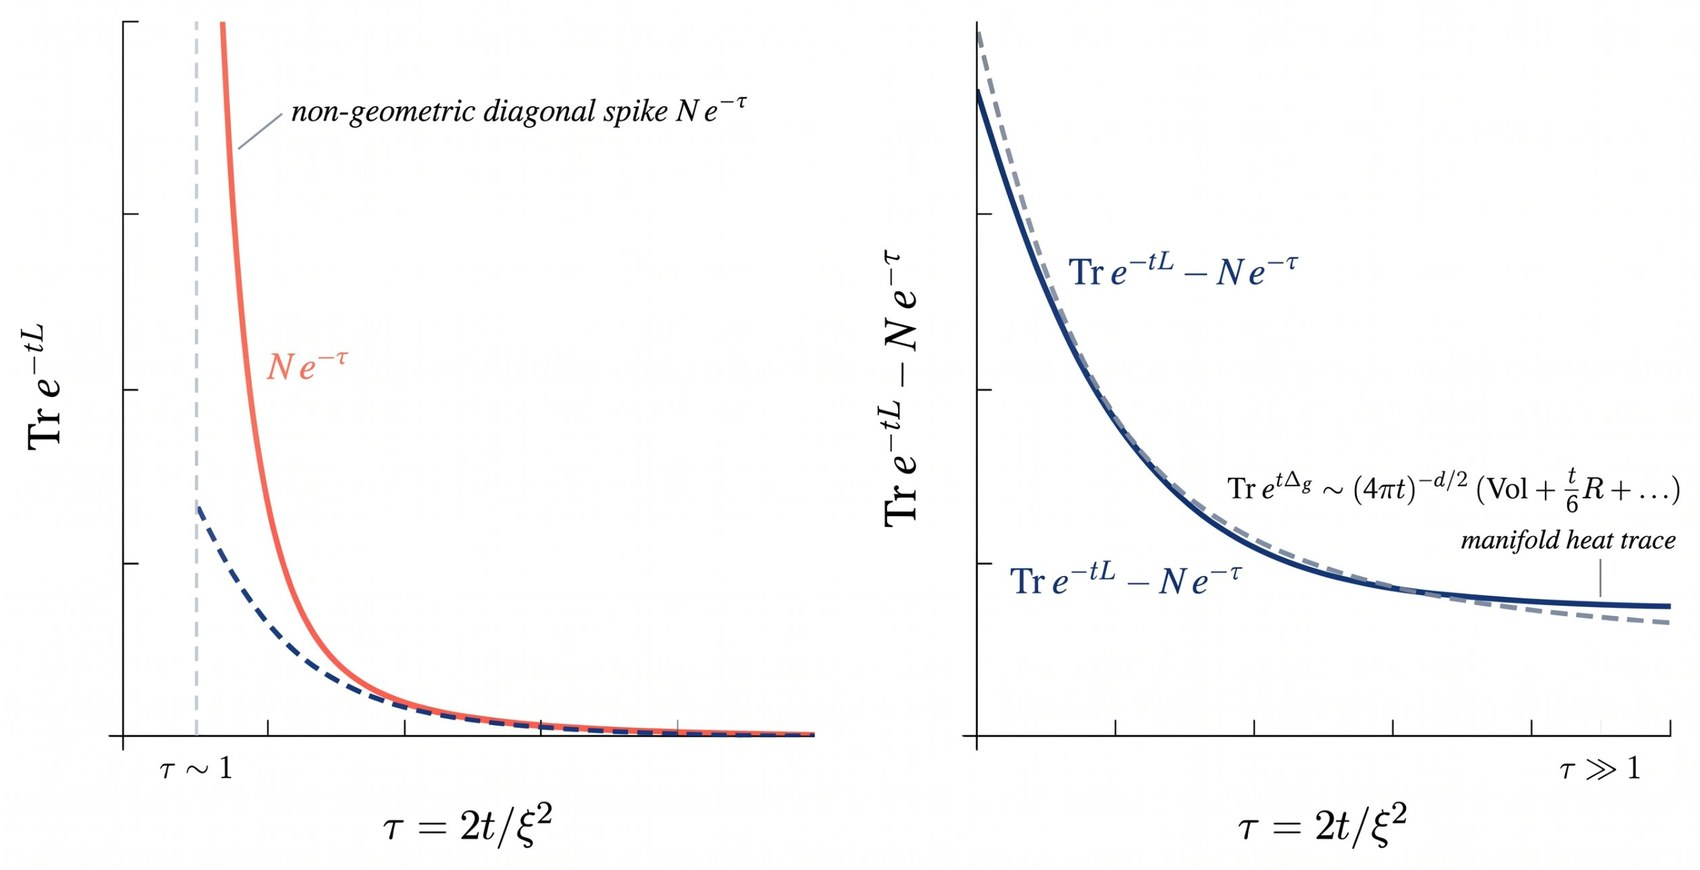
\includegraphics[width=0.86\textwidth]{figures/fig_heat_trace_sketch.jpg}
\caption{Schematic of Theorems~\ref{thm:poisson} and~\ref{thm:trace}, for $c_h=1$. Left: the graph heat trace contains the term $Ne^{-\tau}$ of the walkers that have not moved; it is bounded by $N$ but dominates the trace for $\tau\sim1$. Right: after its subtraction the trace follows the heat trace of the manifold for $\tau\gg1$. Not drawn from data; measured values are in Appendix~\ref{app:heat} and Figure~\ref{fig:rate}.}\label{fig:heatsketch}
\end{figure}

Figure~\ref{fig:heatsketch} illustrates the statement.

\begin{theorem}[Convergence of the heat trace]\label{thm:trace}
Let Assumption~\ref{ass:profile} hold with $d\ge2$, and let $\xi_N\to0$ with $\varepsilon_N/\xi_N\to0$. Then almost surely, for every $t>0$,
\begin{equation}\label{eq:tracesub}
\lim_{N\to\infty}\big(\Tr e^{-t\Lc}-Ne^{-\tau}\big)=\Tr e^{t\Delta_g}.
\end{equation}
Consequently $\Tr e^{-t\Lc}\to\Tr e^{t\Delta_g}$ if and only if $Ne^{-\tau}\to0$, that is, if and only if $2t/(c_h\xi_N^2)-\log N\to\infty$. Moreover, there are constants $c,C,\kappa>0$ such that almost surely, for all large $N$ and all $t\in(0,1]$ with $\xi_N^2\le c\,t$,
\begin{equation}\label{eq:tracerate}
\big|\Tr e^{-t\Lc}-Ne^{-\tau}-\Tr e^{t\Delta_g}\big|\le C\Big(\frac{\varepsilon_N}{\xi_N}+\frac{\xi_N}{\sqrt t}+\tau^{\frac d2+2}e^{-\kappa\tau}\Big)\,t^{-d/2}.
\end{equation}
\end{theorem}

\begin{proof}
Almost surely the conclusions of Theorem~\ref{thm:eig} and Lemma~\ref{lem:traces} hold for all large $N$. Let $s_a\in[-1,1]$ be the eigenvalues of $S$, so that $\lambda_a^N=\tfrac{2}{c_h\xi^2}(1-s_a)$ and
\[
\Tr e^{-t\Lc}-Ne^{-\tau}=\sum_a\big(e^{-\tau(1-s_a)}-e^{-\tau}\big).
\]
Fix $\kappa\in(0,1)$ so small that $2\kappa/c_h$ is below the constant $c$ of \eqref{eq:eiglow}, and split the modes into the low ones, $1-s_a<\kappa$, and the high ones.

\emph{Low modes.} For these $\lambda_a^N<2\kappa/(c_h\xi^2)<c\,\xi^{-2}$, so \eqref{eq:eiglow} gives $\lambda_a^N\ge c\lambda_a$, and for small $\kappa$ also $\xi\sqrt{\lambda_a}\le c$, so that \eqref{eq:eigrate} applies. By Weyl's law their number $n_{\mathrm{low}}$ is at most $C\xi^{-d}$. With $|e^{-x}-e^{-y}|\le|x-y|e^{-\min(x,y)}$ and $t\le1$,
\[
\sum_{\mathrm{low}}\big|e^{-t\lambda_a^N}-e^{-t\lambda_a}\big|\le C\sum_a\Big(\frac{\varepsilon_N}{\xi}+\xi+\xi\sqrt{\lambda_a}\Big)\,t\lambda_a\,e^{-ct\lambda_a}\le C\Big(\frac{\varepsilon_N}{\xi}+\frac{\xi}{\sqrt t}\Big)\Tr e^{(ct/2)\Delta_g}.
\]
The continuum modes with $a\ge n_{\mathrm{low}}$ have $\lambda_a\ge c\,\xi^{-2}$ by \eqref{eq:eigrate}, hence contribute at most $e^{-ct/2\xi^2}\Tr e^{(t/2)\Delta_g}$, and the subtracted terms of the low modes sum to $n_{\mathrm{low}}\,e^{-\tau}\le C\xi^{-d}e^{-\tau}$.

\emph{High modes.} Write $e^{\tau s}-1=(e^{\tau s}-1-\tau s)+\tau s$. Since $|e^x-1-x|\le\tfrac12x^2e^{\max(x,0)}$ and $s_a\le1-\kappa$,
\[
e^{-\tau}\sum_{\mathrm{high}}\big|e^{\tau s_a}-1-\tau s_a\big|\le\tfrac12\tau^2e^{-\kappa\tau}\,\Tr S^2\le C\,\tau^2e^{-\kappa\tau}\xi^{-d},
\]
and $|\sum_{\mathrm{high}}s_a|\le\Tr P+n_{\mathrm{low}}\le C\xi^{-d}$, so the linear part is at most $C\tau e^{-\tau}\xi^{-d}$.

Since $\xi^{-d}=(c_h\tau/2)^{d/2}t^{-d/2}$ and $\Tr e^{s\Delta_g}\le Cs^{-d/2}$ for $s\le1$, collecting the four contributions gives \eqref{eq:tracerate} after decreasing $\kappa$. The limit \eqref{eq:tracesub} follows for $t\le1$; for $t>1$ the same argument applies with dominated convergence in place of the explicit bound.
\end{proof}

The mechanism is that almost all of the $N$ graph modes sit at $s_a\approx0$, and $\Tr S^2=O(\xi^{-d})$ counts them without a factor $N$. Since $\Tr e^{t\Delta_g}\ge c\,t^{-d/2}$, the bound \eqref{eq:tracerate} is a relative error: the subtracted graph trace reproduces the heat trace in the whole regime
\begin{equation}\label{eq:hier}
\varepsilon_N\ll\xi,\qquad \xi^2\ll t\ll\Lcurv^2 ,
\end{equation}
without any logarithm, and the only obstruction to convergence of the unsubtracted trace is the explicit term $Ne^{-\tau}$. The sharper relative rate $O(\xi^2/t)$ suggested by \eqref{eq:leading} is proven in Appendix~\ref{app:rate} for the sampled graph on a flat torus, with the sharp coefficient and almost surely, when $N\xi_N^{d+6}/\log N\to\infty$ (Corollary~\ref{cor:kernel-trace}; Theorem~\ref{thm:jointpoly} is an earlier and weaker version); in the full regime of Theorem~\ref{thm:trace} and on other manifolds it remains open (Section~\ref{sec:open}).

Appendix~\ref{app:heat} develops these two theorems further. It identifies the coefficients of the Poisson series as return moments and shows that the small-$\tau$ behaviour of the trace is fixed by the conventions of the graph (Proposition~\ref{prop:moments}); it sharpens the bounds of Theorem~\ref{thm:poisson} to the chain \eqref{eq:chain}, in which the non-geometric part of the trace appears as the number of walkers that have never left their node (Proposition~\ref{prop:heatbounds}); and it shows that the limit in Theorem~\ref{thm:trace} does not depend on which of the few-step terms are subtracted, in particular not on the self-loops, because the geometric content is carried by the walks with between $\tau/2$ and $2\tau$ steps (Corollary~\ref{cor:subtractions} and \eqref{eq:window}). Section~\ref{app:rate} treats the rate: for the walk whose step is the heat kernel the subtracted trace is the Poisson average of the heat trace, its relative deviation is $d(d+2)/8\tau+O(\tau^{-2})$, of the order $\xi^2/t$ and not smaller (Theorem~\ref{thm:rate}), whereas the trace $\Tr P^k$ of the walk in discrete time has no such term and needs no subtraction (Proposition~\ref{prop:discrete}). The deviation can be removed by a correction (Theorem~\ref{thm:corrected}), for other profiles its coefficient is multiplied by a fourth-moment ratio (Theorem~\ref{thm:profile}), and the sampled graph converges to this case for $N\to\infty$ at fixed $\xi$ (Theorem~\ref{thm:fixedxi}, Corollary~\ref{cor:torus}). For the flat torus with the Gaussian profile the appendix also treats $N\to\infty$ and $\xi_N\to0$ jointly: the entries of the powers of the sampled walk are compared with the heat kernel uniformly in the number of steps (Theorem~\ref{thm:kernel}), which gives the rate $\xi^2/t$ with the sharp coefficient almost surely for $N\xi_N^{d+6}/\log N\to\infty$ (Corollary~\ref{cor:kernel-trace}), in probability for $N\xi_N^{d+4}/\log N\to\infty$ in dimensions one and two (Corollary~\ref{cor:secondstage}) and, by a comparison in the mean over one index, in every dimension (Corollary~\ref{cor:secondstage-alld}), and an estimate of the eigenvalues that is uniform in the index (Theorems~\ref{thm:eigtorus}, \ref{thm:eigtorus-l1}); these statements are recent and their status is recorded in Table~\ref{tab:status}. The finite and order-theoretic parts of these statements have been checked by machine (Remark~\ref{rem:lean}).

\begin{corollary}[Curvature invariants]\label{cor:curv}
On a closed Riemannian $d$-manifold, as $t\to0^+$ \cite{Gilkey},
\begin{equation}\label{eq:heat}
\begin{split}
\Tr e^{t\Delta_g}=(4\pi t)^{-d/2}\Big[&\Vol(\M)+\frac t6\int R\,\dd V\\
&+\frac{t^2}{360}\int\big(5R^2-2|\Ric|^2+2|\Riem|^2\big)\,\dd V+O(t^3)\Big].
\end{split}
\end{equation}
For $d=3$, $|\Riem|^2=4|\Ric|^2-R^2$ pointwise, and the quadratic integrand is $R^2/120+|\Ric|^2/60$. For $d=4$ the Chern--Gauss--Bonnet theorem gives
\begin{equation}\label{eq:d4}
\Tr e^{t\Delta_g}=\int\!\dd^4x\sqrt g\,\Big[\frac{1}{16\pi^2t^2}+\frac{R}{96\pi^2t}+\frac{1}{16\pi^2}\Big(\frac{R^2}{120}+\frac{R_{\mu\nu}R^{\mu\nu}}{60}\Big)\Big]+\frac{\chi(\M)}{90}+O(t).
\end{equation}
By Theorem~\ref{thm:trace} these quantities are determined by the correlation data in the regime \eqref{eq:hier}.
\end{corollary}

\subsection{Reconstruction from near-isometric data}\label{sec:window}

\begin{figure}[t]
\centering
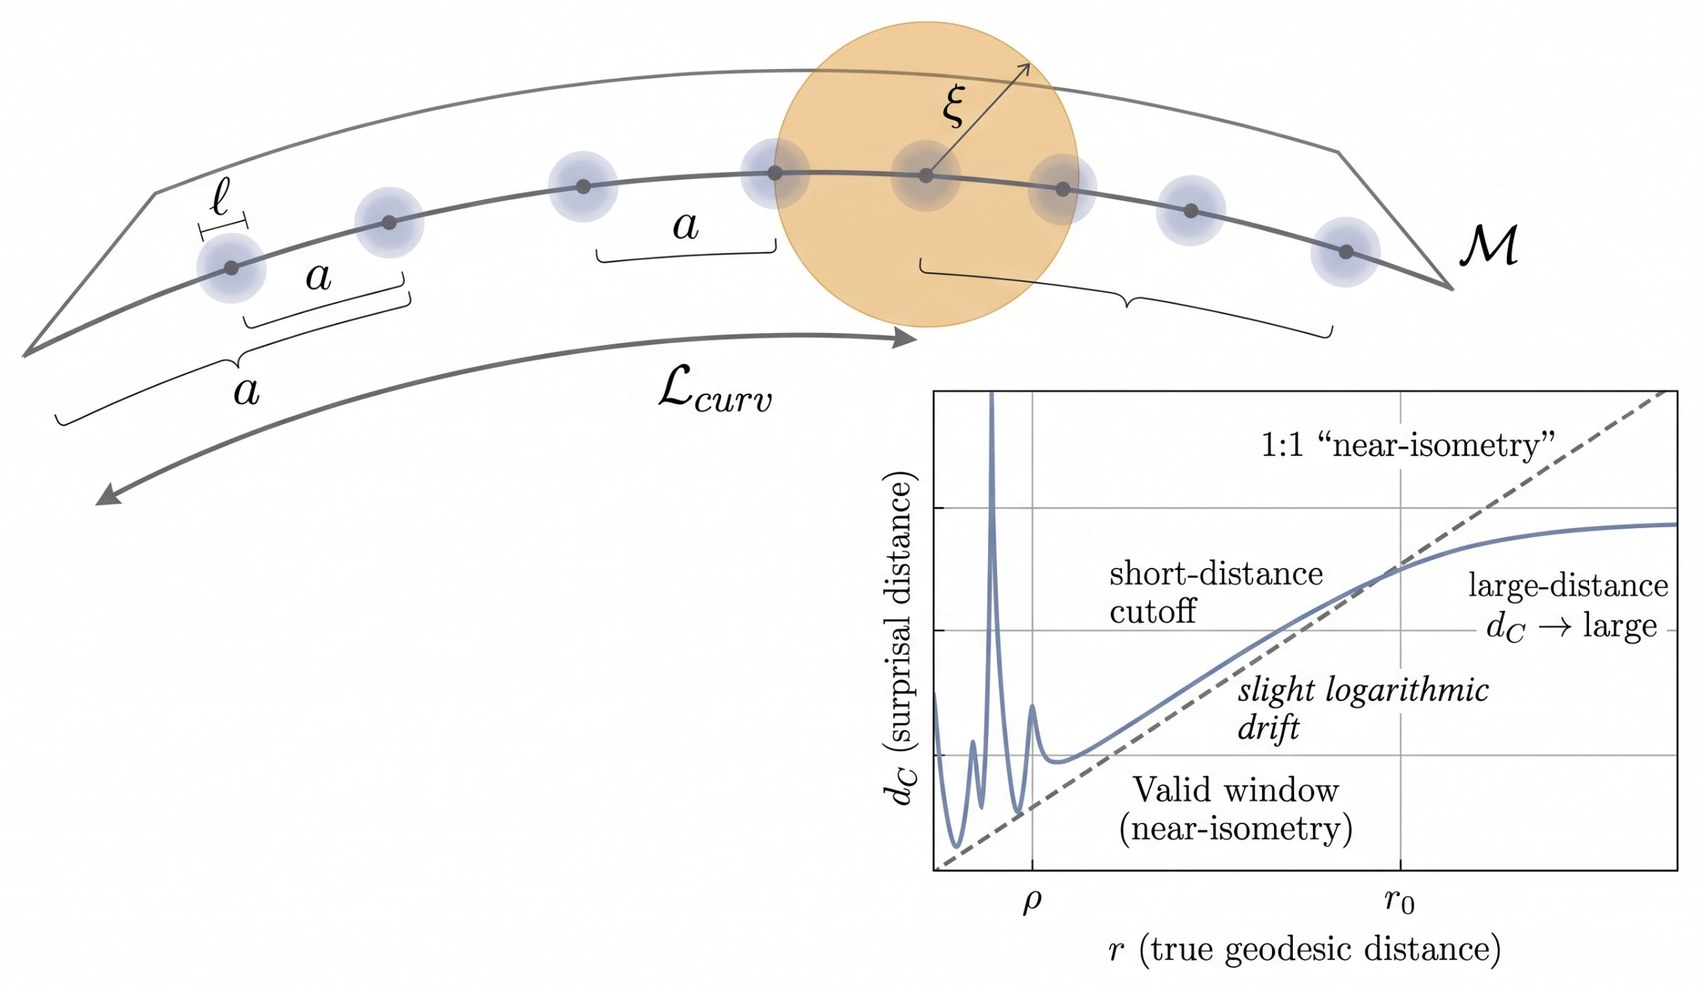
\includegraphics[width=0.82\textwidth]{figures/fig_scales.jpg}
\caption{The scales of the reconstruction. Top: nodes of size $\ell$ at a typical spacing $a$ (of the order of $\varepsilon_N$) on $\M$, the kernel scale $\xi$, and the curvature scale $\Lcurv$. Inset: the surprisal distance $d_C$ against the true distance $r$. Hypothesis~\ref{hyp:window} requires near-isometry only on the window $\rho\le r\le r_0$; below $\rho$ nothing is assumed, and beyond $r_0$ only that $d_C$ is large. Schematic; for the free field $d_C$ keeps growing beyond $r_0$, with the logarithmic drift of Corollary~\ref{cor:drift}.}\label{fig:scales}
\end{figure}

Proposition~\ref{prop:stab} requires control of the kernel on all pairs. Correlation data do not provide this at short distances, where the decay law is not valid and the modes of neighbouring nodes may even overlap. The following statement needs no information below a scale $\rho$ and only a lower bound at large distances. Throughout this subsection $d\ge2$, $d_{ij}=d_g(x_i,x_j)$, and the reference kernel is the Gaussian one with the true distances, $K_{ij}=\exp(-d_{ij}^2/2\xi^2)$, $K_{ii}=1$; this is Assumption~\ref{ass:profile} with $h(s)=e^{-s^2/2}$, $m_0=(2\pi)^{d/2}$ and $c_h=1$.

\begin{hypothesis}[Near-isometry on a window]\label{hyp:window}
A symmetric matrix $d_C(i,j)\ge0$, $i\ne j$, satisfies the hypothesis with parameters $\rho\ge0$, $\Delta\ge0$, $r_0>0$, $r_1>0$ if
\begin{enumerate}[label=\textup{(W\arabic*)}]
\item $|d_C(i,j)-d_{ij}|\le\Delta$ whenever $\rho\le d_{ij}\le r_0$;
\item $d_C(i,j)\ge r_1$ whenever $d_{ij}>r_0$;
\item no condition is imposed on pairs with $d_{ij}<\rho$.
\end{enumerate}
\end{hypothesis}

Given such a matrix let $\tilde K_{ij}=\exp(-d_C(i,j)^2/2\xi^2)$, $\tilde K_{ii}=1$, and let $\tilde q_i$, $\tilde W_{ij}$, $\tilde D_i$, $\tilde\Lc$ and $\tilde\lambda^N_k$ be built from $\tilde K$ as in \eqref{eq:W}, \eqref{eq:L} with $c_h=1$. We write $\mathcal D(u)=\sum_{i,j}W_{ij}(u_i-u_j)^2$ and $\tilde{\mathcal D}(u)=\sum_{i,j}\tilde W_{ij}(u_i-u_j)^2$.

\begin{proposition}[Windowed stability]\label{prop:window}
Let $d\ge2$ and $r_0,r_1>0$. There are constants $c,C>0$, depending only on $(\M,g)$, $\mu$, $r_0$ and $r_1$, with the following property. Let $\xi\le c$, $N\xi^d\ge C\log N$, $\rho\le\xi/4$, and put
\begin{equation}\label{eq:vartheta}
\vartheta=\frac\Delta\xi\sqrt{\ln(1/\xi)}+\Big(\frac\rho\xi\Big)^d+\frac{\log N}{N\xi^d}+\xi^2 .
\end{equation}
Then there is an event of probability at least $1-CN^{-2}$, depending only on the points, on which the following holds for every matrix $d_C$ satisfying Hypothesis~\ref{hyp:window} with parameters $(\rho,\Delta,r_0,r_1)$, provided $\vartheta\le c$: for all $i$ and all $u\in\R^N$,
\begin{gather}
(1-C\vartheta)D_i\le\tilde D_i\le(1+C\vartheta)D_i,\qquad c\,\xi^d\le\tilde q_i\le C\xi^d,\label{eq:winD}\\
\big|\tilde{\mathcal D}(u)-\mathcal D(u)\big|\le C\vartheta\,\Big(\mathcal D(u)+\xi^2\sum_iD_iu_i^2\Big).\label{eq:winE}
\end{gather}
Consequently $|\tilde\lambda^N_k-\lambda^N_k|\le C\vartheta\,(\lambda^N_k+1)$ for all $0\le k\le N-1$.
\end{proposition}

\begin{theorem}[Reconstruction from near-isometric data]\label{thm:window}
Let $d\ge2$ and let the points be sampled as in Assumption~\ref{ass:profile} (only the manifold and the density $\mu$ enter). Let $\xi_N\to0$ with $\varepsilon_N/\xi_N\to0$, and let $d_C=d_C^{(N)}$ be matrices that, almost surely for all large $N$, satisfy Hypothesis~\ref{hyp:window} with fixed $r_0,r_1$ and parameters $\rho_N\le\xi_N/4$, $\Delta_N$ such that
\begin{equation}\label{eq:varthetaN}
\vartheta_N:=\frac{\Delta_N}{\xi_N}\sqrt{\ln(1/\xi_N)}+\Big(\frac{\rho_N}{\xi_N}\Big)^d\longrightarrow0 .
\end{equation}
Then almost surely, for all large $N$, with constants depending only on $(\M,g)$, $\mu$, $r_0$, $r_1$:
\begin{enumerate}[label=\textup{(\roman*)}]
\item for every $k\ge1$ with $\xi_N\sqrt{\lambda_k}\le c$,
\[
\big|\tilde\lambda^N_k-\lambda_k\big|\le C\Big(\frac{\varepsilon_N}{\xi_N}+\xi_N\big(1+\sqrt{\lambda_k}\big)+\vartheta_N\Big)\lambda_k ,
\]
and $\tilde\lambda^N_k\ge c\min\{\lambda_k,\xi_N^{-2}\}$ for all $1\le k\le N-1$, eigenvalues counted with multiplicity;
\item the conclusions of Theorems~\ref{thm:evec} and~\ref{thm:cluster} hold for the eigenvectors of $\tilde\Lc$, weighted by $\tilde\pi_i=\tilde D_i/\sum_k\tilde D_k$, with $\varepsilon_N/\xi_N+\xi_N$ replaced by $\varepsilon_N/\xi_N+\xi_N+\vartheta_N$;
\item for every $t>0$, with $\tau=2t/\xi_N^2$, $\Tr e^{-t\tilde\Lc}-Ne^{-\tau}\to\Tr e^{t\Delta_g}$, and the bound \eqref{eq:tracerate} holds with $\varepsilon_N/\xi_N$ replaced by $\varepsilon_N/\xi_N+\vartheta_N$.
\end{enumerate}
\end{theorem}

The proofs are in Appendix~\ref{app:e2e}. Part (i) is proven in full; for (ii) and (iii) the appendix lists the places where the two-sided bound \eqref{eq:twosided} enters the proofs of Theorems~\ref{thm:evec}, \ref{thm:cluster} and~\ref{thm:trace} and shows that \eqref{eq:winD}, \eqref{eq:winE} suffice there; these proofs have not been rewritten line by line.

\begin{remark}\label{rem:window}
(a) Proposition~\ref{prop:stab} alone does not cover the short pairs: its second condition would require $(\rho/\xi)^d\ll\xi^2$. A chaining argument removes this restriction and needs no information at all on the kernel below the scale $\rho$.
(b) The additive constant of the surprisal distance matters. Replacing $C_0$ by $e^{\kappa}C_0$ in \eqref{eq:surprisal} shifts $d_C$ by $\kappa\xi_0$; this is harmless only if $\kappa\xi_0\sqrt{\ln(1/\xi)}\ll\xi$. A shift of order $\xi$ is still a monotone profile in the sense of Assumption~\ref{ass:profile}, but with a different constant $c_h$, which must then be known in order to normalise $\Lc$.
(c) Hypothesis~\ref{hyp:window} is an approximate isometry with an additive error on a window. It is not in conflict with Corollary~\ref{cor:drift}: the relative form with error $O(r/\Lcurv)$ fails for free fields, the additive form holds with $\Delta=O(\xi_0\ln(1/\xi_0))$, see Theorem~\ref{thm:e2e}.
(d) Theorem~\ref{thm:window} is purely geometric and makes no reference to fields.
\end{remark}

\section{Microscopic realisation: Gaussian states}\label{sec:gauss}

We now ask when Assumption~\ref{ass:profile} can hold, for the simplest class of states.

\begin{proposition}[Classical Gaussian variables]\label{prop:classical}
Let $(Y_A,Y_B)$ be jointly Gaussian with invertible covariance and $\mathsf R=\Sigma_A^{-1/2}\Sigma_{AB}\Sigma_B^{-1/2}$. Then
\begin{equation}
I(Y_A:Y_B)=-\tfrac12\ln\det(1-\mathsf R^{T}\mathsf R),\qquad \tfrac12\|\mathsf R\|_F^2\le I\le\frac{\tfrac12\|\mathsf R\|_F^2}{1-\|\mathsf R\|_{\mathrm{op}}^2}.
\end{equation}
\end{proposition}

\begin{proof}
For Gaussian variables $I=\tfrac12\ln(\det\Sigma_A\det\Sigma_B/\det\Sigma)$, and the Schur complement gives
\[\det\Sigma=\det\Sigma_A\,\det\Sigma_B\,\det(1-\mathsf R^T\mathsf R).\] The eigenvalues $\rho_i^2$ of $\mathsf R^T\mathsf R$ lie in $[0,1)$, and $x\le-\ln(1-x)\le x/(1-x)$ there.
\end{proof}

\begin{proposition}[Two bosonic modes]\label{prop:twomode}
Let $(\phi_A,\pi_A)$, $(\phi_B,\pi_B)$ be two modes in a Gaussian state with $\langle\phi_A^2\rangle=\langle\phi_B^2\rangle=x_0$, $\langle\pi_A^2\rangle=\langle\pi_B^2\rangle=p_0$, $\langle\phi_A\phi_B\rangle=x$, $\langle\pi_A\pi_B\rangle=p$ and vanishing symmetrised $\phi\pi$ correlations. Let $\nu=\sqrt{x_0p_0}>\tfrac12$, $f(\nu)=(\nu+\tfrac12)\ln(\nu+\tfrac12)-(\nu-\tfrac12)\ln(\nu-\tfrac12)$, so that $f'(\nu)=\ln\frac{\nu+1/2}{\nu-1/2}$, and $\varepsilon=x_0p+p_0x$. Then, as $(x,p)\to0$,
\begin{equation}\label{eq:twomode}
I(A:B)=\varepsilon^2\Big[\frac{f'(\nu)}{4\nu^3}+\frac{1}{4\nu^2(\nu^2-\tfrac14)}\Big]-\frac{f'(\nu)}{\nu}\,xp+O\big(|(x,p)|^4\big).
\end{equation}
\end{proposition}

\begin{proof}
The $\phi$- and $\pi$-covariance blocks are $2\times2$ matrices with equal diagonal entries and commute, so the symplectic eigenvalues of the pair are $\nu_\pm=\sqrt{(x_0\pm x)(p_0\pm p)}$ and that of one mode is $\nu$. The entropy of a Gaussian state is the sum of $f$ over its symplectic eigenvalues, hence $I=2f(\nu)-f(\nu_+)-f(\nu_-)$. From $\nu_\pm^2=\nu^2\pm\varepsilon+xp$ we get $\nu_\pm-\nu=\pm\varepsilon/2\nu+xp/2\nu-\varepsilon^2/8\nu^3+O(3)$. Expanding $f$ to second order with $f''(\nu)=-1/(\nu^2-\tfrac14)$ gives \eqref{eq:twomode}. $I$ is even under $(x,p)\mapsto(-x,-p)$, which exchanges $\nu_+$ and $\nu_-$, so the remainder is of fourth order.
\end{proof}

\begin{proposition}[Several modes per node]\label{prop:multimode}
Let $A$ and $B$ consist of $M$ modes each, in a Gaussian state with covariance matrix $\sigma=\big(\begin{smallmatrix}\sigma_A&\mathsf C\\ \mathsf C^{T}&\sigma_B\end{smallmatrix}\big)$, and let $\mathsf R_\phi$ be the matrix $\mathsf R$ of Proposition~\ref{prop:classical} for the configuration variables $\phi_A,\phi_B$. Then
\begin{equation}
I(A:B)\ge-\tfrac12\ln\det(1-\mathsf R_\phi^{T}\mathsf R_\phi)\ge\tfrac12\|\mathsf R_\phi\|_F^2 .
\end{equation}
Moreover, for every compact set $\mathcal K$ of pairs $(\sigma_A,\sigma_B)$ with all symplectic eigenvalues larger than $\tfrac12$ there are $\rho_0,C>0$ such that $I(A:B)\le C\|\mathsf C\|_F^2$ whenever $(\sigma_A,\sigma_B)\in\mathcal K$ and $\|\mathsf C\|_F\le\rho_0$.
\end{proposition}

\begin{proof}
Measuring $\phi_A$ and $\phi_B$ is a local operation, under which mutual information does not increase; the outcome is the classical Gaussian pair of Proposition~\ref{prop:classical}. For the upper bound, the entropy of a Gaussian state is $\tfrac12\Tr\,g(-(J\sigma)^2)$ with $g(s)=f(\sqrt s)$ analytic on $s>\tfrac14$, where $J$ is the symplectic matrix; hence $I$ is a real-analytic function of $\mathsf C$ near $\mathsf C=0$, uniformly on $\mathcal K$. Since $I\ge0$ and $I=0$ at $\mathsf C=0$, its gradient vanishes there, and Taylor's formula gives $I\le\tfrac12\sup\|\dd^2I\|\,\|\mathsf C\|_F^2$.
\end{proof}

For nodes with several modes the mutual information is therefore comparable to the squared cross-correlations, and decays as $e^{-2mr}$ times a power, as in the single-mode case; the constants and the power are not determined by this argument.

\begin{theorem}[Decay law]\label{thm:decay}
Consider the vacuum of a free scalar field of mass $m$ on $\R^D$. Let each node carry the mode $\phi(f_a),\pi(f_a)$ with $f_a=f(\cdot-a)$, $f$ radial, supported in a ball of radius $\ell$, $\int f^2=1$. For two nodes at distance $r\to\infty$,
\begin{equation}\label{eq:decay}
I(r)=c_0\,F^4\,\frac{m^{D-2}}{4(2\pi)^D}\;r^{-D}e^{-2mr}\Big[1+O\Big(\frac1{mr}\Big)+O\Big(\frac{\ell+m\ell^2}{r}\Big)\Big],
\end{equation}
where $F=\int f(u)e^{m\,n\cdot u}\,\dd u$ (independent of the unit vector $n$) and $c_0=p_0^2\big[f'(\nu)/4\nu^3+1/(4\nu^2(\nu^2-\tfrac14))\big]$.
\end{theorem}

The proof is in Appendix~\ref{app:decay}. On a flat torus much larger than $r$ the same law holds up to exponentially small image terms, which provides a closed manifold as required by Assumption~\ref{ass:profile}. The rate $2m$ is the square of the clustering rate of the two-point function \cite{AHR,Fredenhagen,HastingsKoma}; the quadratic dependence on the correlator is the massive counterpart of Cardy's result for conformal theories \cite{Cardy}. The lower bound $I\ge\tfrac12(\text{correlation})^2$ holds for arbitrary states \cite{WVHC}; an upper bound of the same order is not available for interacting systems, and for those \eqref{eq:decay} is a conjecture.

\begin{corollary}[Logarithmic drift]\label{cor:drift}
With $\xi_0=1/(2m)$, the surprisal distance \eqref{eq:surprisal} of the states in Theorem~\ref{thm:decay} is
\begin{equation}
d_C=r+D\,\xi_0\ln r+\mathrm{const}+O\big(\xi_0/(mr)\big).
\end{equation}
Hence $d_C/r\to1$ only logarithmically, and $d_C$ is not a metric with relative error $O(r/\Lcurv)$. Nevertheless $C=F(r)$ with a single monotone $F$, so Assumption~\ref{ass:profile} holds, with $h(s)=\exp\!\big(-(\xi s+D\xi_0\ln(\xi s/r_0))^2/2\xi^2\big)$ for $\xi s>r_0$.
\end{corollary}

\begin{remark}[Scales]\label{rem:scales}
The law \eqref{eq:decay} is valid for $r\gg\xi_0$ and $r\gg\ell$, so the kernel must probe distances above $\xi_0$. With node spacing $a$ and \eqref{eq:hier} this gives
\begin{equation}
\ell\lesssim a\ll\xi,\qquad \xi_0\lesssim\xi,\qquad \xi^2\ll t\ll\Lcurv^2 .
\end{equation}
A limit $\xi\to0$ at fixed $\xi_0$ does not exist: the correlation length must shrink with the kernel scale. If $\lambda_0/48\pi^2t$ is read as a squared Planck mass $M_{\mathrm{Pl}}^2$ (Remark~\ref{rem:coeff}), the hierarchy implies $m\gg11\,M_{\mathrm{Pl}}/\sqrt{\lambda_0}$: the field that carries the geometric correlations needs a gap far above the Planck scale, or a very large $\lambda_0$. For the end-to-end statement of Theorem~\ref{thm:e2e} the condition on $\xi_0$ is stronger, $\xi_0\ln(1/\xi_0)\sqrt{\ln(1/\xi)}\ll\xi$.
\end{remark}

\subsection{Curved backgrounds}\label{sec:curved}

Let now $(\M,g)$ be a closed Riemannian manifold of dimension $d$ and consider the free field of mass $m$ on the ultrastatic spacetime $\R\times\M$ with metric $-\dd t^2+g$. In its ground state the equal-time correlators are $X=\tfrac12A^{-1/2}$ and $P=\tfrac12A^{1/2}$ with $A=-\Delta_g+m^2$. For real $\sigma$ let $k_\sigma(x,y)$, $x\ne y$, denote the integral kernel of $A^{-\sigma}$ off the diagonal. For $\sigma>0$,
\begin{equation}\label{eq:ksigma}
k_\sigma(x,y)=\frac{1}{\Gamma(\sigma)}\int_0^\infty s^{\sigma-1}e^{-m^2s}\,p_s(x,y)\,\dd s ,
\end{equation}
where $p_s$ is the heat kernel of $(\M,g)$; since $p_s(x,y)$ vanishes to infinite order as $s\to0$ for $x\ne y$, both sides are entire in $\sigma$ and \eqref{eq:ksigma} holds for all $\sigma$, with $1/\Gamma(-\tfrac12)=-1/2\sqrt\pi$. In flat space the same formula gives
\begin{equation}\label{eq:kflat}
k^{\mathrm{flat}}_\sigma(r)=\frac{2^{1-\sigma}}{(2\pi)^{d/2}\Gamma(\sigma)}\Big(\frac mr\Big)^{\frac d2-\sigma}K_{\frac d2-\sigma}(mr),
\end{equation}
which for $\sigma=\pm\tfrac12$ are the correlators used in Theorem~\ref{thm:decay}. Let $u_0,u_1$ be the first two coefficients of the heat-kernel expansion $p_s\sim(4\pi s)^{-d/2}e^{-d_g^2/4s}\sum_js^ju_j$. With $y=\exp_x(v)$ and $J_x$ the Jacobian of $\exp_x$,
\begin{equation}\label{eq:u0}
u_0(x,y)=J_x(v)^{-1/2}=1+\tfrac1{12}\Ric_x(v,v)+O(|v|^3),\qquad u_1(x,x)=\tfrac16R(x).
\end{equation}

\begin{theorem}[Correlators on a curved background]\label{thm:curved}
Let $r_0<\mathrm{inj}(\M)$ and $\sigma\in\{-\tfrac12,\tfrac12,1\}$. There are constants $m_0$ and $C$, depending on $(\M,g)$, $r_0$ and $\sigma$, such that for all $m\ge m_0$ and all $x,y$ with $1/m\le r=d_g(x,y)\le r_0$,
\begin{equation}\label{eq:curved}
\Big|\frac{k_\sigma(x,y)}{k^{\mathrm{flat}}_\sigma(r)}-u_0(x,y)-\frac{r}{2m}\,\rho_\sigma(mr)\,u_1(x,y)\Big|\le C\,\frac{r^2}{m^2},
\qquad \rho_\sigma(z)=\frac{K_{|d/2-\sigma-1|}(z)}{K_{|d/2-\sigma|}(z)} .
\end{equation}
The function $\rho_\sigma$ is bounded on $[1,\infty)$ and $\rho_\sigma(z)\to1$ as $z\to\infty$.
\end{theorem}

The proof (Appendix~\ref{app:curved}) inserts the heat-kernel asymptotics in the strong, multiplicative form of Ludewig \cite{Ludewig} into \eqref{eq:ksigma}; the usual additive remainder would not suffice, because the correlator is exponentially small. On the unit sphere $S^3$ everything is explicit: the heat kernel is $e^{s}(4\pi s)^{-3/2}\sum_{n\in\mathbb Z}\frac{\gamma+2\pi n}{\sin\gamma}e^{-(\gamma+2\pi n)^2/4s}$ with $\gamma=d_g(x,y)$, so that $u_0=u_1=\gamma/\sin\gamma$ and

\begin{figure}[t]
\centering
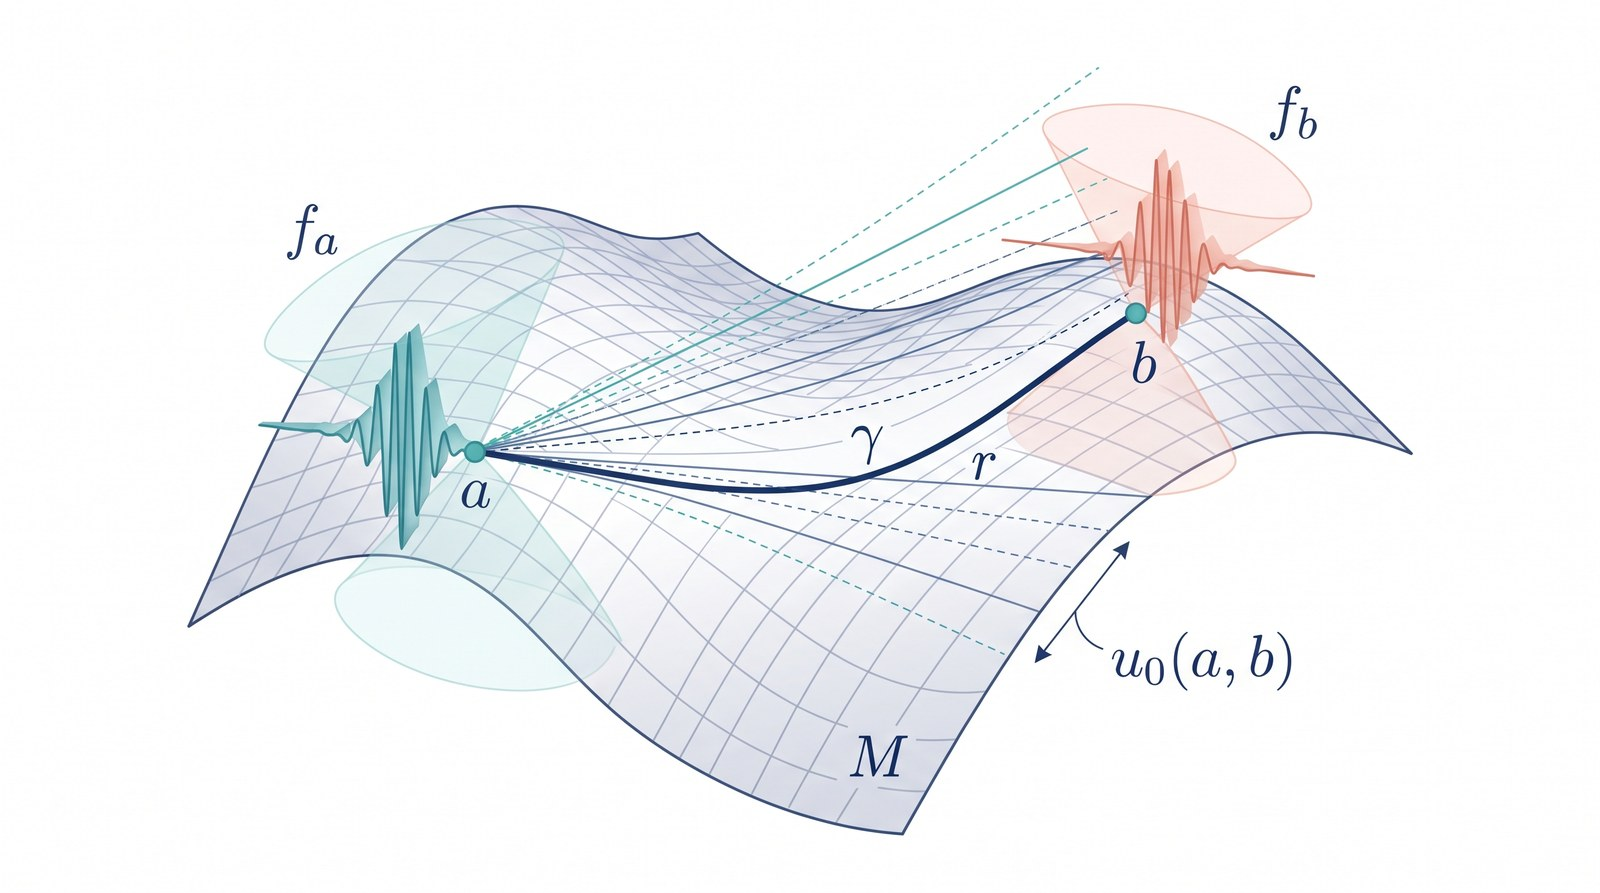
\includegraphics[width=0.80\textwidth]{figures/fig_modes_geodesic.jpg}
\caption{Two nodes $a$ and $b$ of the slice $\M$ with their localised modes $f_a$, $f_b$, joined by the geodesic $\gamma$ of length $r$. The correlators of the modes, and with them the mutual information, depend on $r$ through the flat profile (Theorem~\ref{thm:decay}) and on the geometry near $\gamma$ through the factor $u_0(a,b)$ of Theorem~\ref{thm:curved}. Schematic, produced as stated in the caption of Figure~\ref{fig:sketch}: the cones and the fan of lines have no quantitative meaning, and $u_0$ is a dimensionless factor, not the length indicated by the double arrow.}\label{fig:modes}
\end{figure}
\begin{equation}
X(\gamma)=\frac{\mu\,K_1(\mu\gamma)}{4\pi^2\sin\gamma}+\text{images},\qquad \mu^2=m^2-1,
\end{equation}
in agreement with \eqref{eq:curved}; see Appendix~\ref{app:num}.

Thus curvature enters the correlators at leading order through the Van Vleck factor $u_0$, anisotropically and at relative order $r^2/\Lcurv^2$, and the gap produces a further relative correction of order $r/(m\Lcurv^2)$.

\paragraph{Geodesic modes} We now make the modes explicit. In the rest of this subsection $(\M,g)$ is closed of dimension $d\ge2$, $r_0<\mathrm{inj}(\M)$ and $m\ge1$. The profile $\chi:\R^d\to[0,\infty)$ is smooth, radial, supported in the unit ball, with $\int\chi^2=1$; positivity is used to turn relative errors of kernels into relative errors of integrals. For $a\in\M$ and $0<\ell\le\min\{1/m,r_0/4\}$ let
\begin{equation}\label{eq:geomode}
f_a\big(\exp_a(u)\big)=\ell^{-d/2}\,J_a(u)^{-1/2}\,\chi(u/\ell),\qquad f^\flat(u)=\ell^{-d/2}\chi(u/\ell)\quad(u\in\R^d),
\end{equation}
and let $x_0^\flat=\tfrac12\langle f^\flat,(-\Delta+m^2)^{-1/2}f^\flat\rangle$, $p_0^\flat=\tfrac12\langle f^\flat,(-\Delta+m^2)^{1/2}f^\flat\rangle$ be the flat single-mode data. With $\Phi(s)=\int\chi(w)e^{sw_1}\dd w$ put $F=\ell^{d/2}\Phi(m\ell)$. Constants $c,C$ depend only on $(\M,g)$, $r_0$ and $\chi$.

\begin{proposition}[Geodesic modes]\label{prop:modes}
Under these assumptions $\|f_a\|_{L^2(\M)}=1$, and:
\begin{enumerate}[label=\textup{(\roman*)}]
\item the single-mode data $x_0(a)=\langle f_a,Xf_a\rangle$, $p_0(a)=\langle f_a,Pf_a\rangle$ satisfy
\[
\Big|\frac{x_0(a)}{x_0^\flat}-1\Big|+\Big|\frac{p_0(a)}{p_0^\flat}-1\Big|\le C\,\omega,\qquad\omega:=\frac\ell m+e^{-m^2};
\]
\item there is $m_0$ such that for $m\ge m_0$ and nodes with $3/m\le r=d_g(a,b)\le r_0-2\ell$,
\begin{gather*}
x_{ab}=F^2X^{\mathrm{flat}}(r)\,u_0(a,b)\,(1+\theta_x),\qquad p_{ab}=F^2P^{\mathrm{flat}}(r)\,u_0(a,b)\,(1+\theta_p),\\
|\theta_x|+|\theta_p|\le C\Big(\frac rm+\frac{\ell+m\ell^2}{r}+\ell^2+m\,r\,\ell^2\Big).
\end{gather*}
\end{enumerate}
\end{proposition}

Mutual information is invariant under $(\phi,\pi)\mapsto(\phi/\sqrt\ell,\sqrt\ell\,\pi)$ at every node. We write $\hat x_0=x_0/\ell$, $\hat p_0=\ell p_0$, $\hat x=x/\ell$, $\hat p=\ell p$. The flat data $\sigma_*(s)=(\hat x_0^\flat,\hat p_0^\flat)$, with $\hat x_0^\flat=\tfrac12\langle\chi,(-\Delta+s^2)^{-1/2}\chi\rangle$ and $\hat p_0^\flat=\tfrac12\langle\chi,(-\Delta+s^2)^{1/2}\chi\rangle$, depend continuously on $s=m\ell\in[0,1]$ (for $d\ge2$ the first is finite at $s=0$), and $\nu^2=\hat x_0^\flat\hat p_0^\flat>\tfrac14$ by the Cauchy--Schwarz inequality, strictly because a compactly supported $\chi$ is not an eigenfunction. For single-mode data $\sigma_A=(\hat x_A,\hat p_A)$, $\sigma_B=(\hat x_B,\hat p_B)$ and a cross block $\mathsf c=(\hat x,\hat p)$, all $\phi\pi$ correlations vanishing, let $I(\sigma_A,\sigma_B;\mathsf c)$ be the mutual information of the two modes.

\begin{corollary}[Mutual information of geodesic modes]\label{cor:curvedMI}
Let $\hat{\mathsf c}_0(r)=\big(F^2X^{\mathrm{flat}}(r)/\ell,\ \ell F^2P^{\mathrm{flat}}(r)\big)$ and $I_0(r)=I(\sigma_*,\sigma_*;\hat{\mathsf c}_0(r))$ with $\sigma_*=\sigma_*(m\ell)$, the flat two-mode mutual information. There are $m_0,C_1,C$ such that for $m\ge m_0$:
\begin{enumerate}[label=\textup{(\roman*)}]
\item for $mr\ge C_1$, with $c_1$ the coefficient of $\varepsilon^2$ in \eqref{eq:twomode} at $\sigma_*$ and
\begin{equation}\label{eq:Aml}
\begin{gathered}
\mathsf A(m,\ell)=\frac{c_1\,(p_0^\flat)^2F^4\,m^{2d-2}}{4(2\pi)^d},\\
I_0(r)=\mathsf A(m,\ell)\,(mr)^{-d}e^{-2mr}\big(1+\theta(r)\big),\qquad|\theta(r)|\le\frac{C}{mr}\le\frac12;
\end{gathered}
\end{equation}
\item for nodes with $C_1/m\le r=d_g(a,b)\le r_0-2\ell$,
\begin{gather*}
I(a:b)=I_0(r)\,u_0(a,b)^2\,(1+\beta'_{ab}),\\
|\beta'_{ab}|\le C\Big(\frac rm+\frac{\ell+m\ell^2}{r}+\ell^2+m\,r\,\ell^2+\frac\ell m+e^{-m^2}+(m\ell)^{2d-2}e^{-2mr}\Big),
\end{gather*}
and $u_0(a,b)^2=1+\tfrac16\Ric_a(v,v)+O(r^3)$ for $b=\exp_a(v)$.
\end{enumerate}
\end{corollary}

Thus the correlations on a curved background are a profile of the distance up to the anisotropic factor $u_0^2$ and small errors. Two points need care in the proof (Appendix~\ref{app:e2e}): the single-mode data of two nodes on a curved manifold are not equal, so Proposition~\ref{prop:twomode} does not apply directly, and the quartic remainder of \eqref{eq:twomode} is exponentially small in $mr$ but not $O(r/m)$; it is the last term of the bound for $\beta'_{ab}$. The terms $\ell^2$, $mr\ell^2$, $\ell/m$ and $r/m$ come from curvature only.

\paragraph{The end-to-end statement} Let the field of mass $m$ on $\R\times\M$ be in its ground state and let node $i$ carry the geodesic mode $f_{x_i}$ with radius $\ell$, $m\ell\le1$. We use the surprisal distance \eqref{eq:surprisal} with $\xi_0=1/(2m)$ and $C_0=\mathsf A(m,\ell)$, the prefactor of the flat decay law; $C_{ij}=I(i:j)$ whenever the supports of $f_{x_i},f_{x_j}$ are disjoint.

\begin{theorem}[End-to-end reconstruction for the free field]\label{thm:e2e}
In this setting let $\xi_N\to0$, $m_N\to\infty$ and $\ell_N$ be such that
\begin{enumerate}[label=\textup{(E\arabic*)}]
\item $\varepsilon_N/\xi_N\to0$;
\item $\vartheta_N:=\dfrac{\ln m_N}{m_N\xi_N}\sqrt{\ln(1/\xi_N)}\longrightarrow0$;
\item $\ell_N\le N^{-4/d}$ and $m_N\ell_N\le1$.
\end{enumerate}
Let $\tilde\Lc$ be the operator \eqref{eq:L} with $c_h=1$ built from $C_{ij}=I(i:j)$ via \eqref{eq:surprisal} with $\xi=\xi_N$, $\xi_0=1/(2m_N)$ and $C_0=\mathsf A(m_N,\ell_N)$. Then, almost surely, the modes of distinct nodes have disjoint supports for all large $N$, and conclusions (i)--(iii) of Theorem~\ref{thm:window} hold with $\vartheta_N$ as in \textup{(E2)}. In particular
\[
\tilde\lambda^N_k\longrightarrow\lambda_k\ \text{ for every }k,\qquad\Tr e^{-t\tilde\Lc}-Ne^{-2t/\xi_N^2}\longrightarrow\Tr e^{t\Delta_g}\ \text{ for every }t>0,
\]
and the integrated curvature invariants of Corollary~\ref{cor:curv} are determined by the mutual informations of the ground state.
\end{theorem}

\begin{remark}[Scales]\label{rem:curvedrecon}
(a) The conditions are satisfiable, for instance by $\xi_N=N^{-1/2d}$, $m_N=N^{1/d}$, $\ell_N=N^{-4/d}$.
(b) The hierarchy is $\ell\ll\min_{i\ne j}d_{ij}\ll\varepsilon_N\ll\xi$, $\ \xi_0\ln(1/\xi_0)\sqrt{\ln(1/\xi)}\ll\xi$, $\ \xi^2\ll t$. This is stronger than the condition on $\xi_0$ in Remark~\ref{rem:scales}. The borderline $\xi_0\sim\xi$ is not covered: there the drift is of the size of the kernel scale, the profile is not Gaussian, and $c_h$ depends on the short-distance form of $I_0$.
(c) The price of $\xi_0\ll\xi$ is that the informative pairs, at distance of order $\xi$, have mutual information of order $e^{-\xi/\xi_0}$. The theorem is an identifiability statement, not a statement about noisy data: an error in $C_{ij}$ must be small relative to $C_{ij}$ itself, to the extent that $\xi_0|\delta\ln C_{ij}|\sqrt{\ln(1/\xi)}\ll\xi$.
(d) The condition $\ell_N\le N^{-4/d}$ is forced by independent sampling: the smallest distance between $N$ independent points is of order $N^{-2/d}$, and overlapping modes are not independent subsystems. For well-separated nodes $\ell$ of the order of the spacing would suffice, but Lemma~\ref{lem:transport} would have to be replaced.
(e) Not covered: several modes per node, nodes that are not sampled independently, and interacting fields; for the latter Theorem~\ref{thm:window} applies once \textup{(W1)}, \textup{(W2)} are established.
\end{remark}

\section{Towards dynamics: what the spectral data determine}\label{sec:dyn}

The earlier manuscript proposed field equations by extremising $\lambda_0\Tr e^{-t\Lc}$ together with a matter entropy. We withdraw that ansatz and record what can be proven instead.

\subsection{No stationary metric}

\begin{theorem}\label{thm:nostat}
Let $\nu$ be a nonzero positive measure on $(0,\infty)$ and
\begin{equation}
\Phi_\nu(g)=\int\nu(\dd s)\,\Tr e^{s\Delta_g}.
\end{equation}
Assume that $\Phi_\nu(g)$ and $\int\nu(\dd s)\sum_as\lambda_ae^{-s\lambda_a}$ are finite for every metric $g$. Then neither $\Phi_\nu$ nor $-\Phi_\nu$ has a stationary point on the space of Riemannian metrics of a closed manifold.
\end{theorem}

\begin{proof}
For a constant $\sigma>0$, $\Delta_{\sigma^2g}=\sigma^{-2}\Delta_g$, so $\Phi_\nu(\sigma^2g)=\int\nu(\dd s)\sum_ae^{-s\lambda_a/\sigma^2}$ and
\begin{equation}
\frac{\dd}{\dd\sigma}\Phi_\nu(\sigma^2g)\Big|_{\sigma=1}=\int\nu(\dd s)\sum_a2s\lambda_ae^{-s\lambda_a}>0
\end{equation}
because $\lambda_1>0$. At a stationary point the derivative along every curve of metrics vanishes, in particular along $\sigma\mapsto\sigma^2g$.
\end{proof}

Thus the equation $\delta\Phi=0$ has no solution for the heat trace, for any completely monotone mixture of heat traces, or for the one-loop free energy of a single scalar field (Remark~\ref{rem:induced}), unless a matter term balances the scale derivative or the weight $\nu$ changes sign. This is the functional-analytic form of the statement that the scale is not dynamical; Chamseddine and Connes restore scale invariance of the spectral action by introducing a dilaton \cite{CC06}.

\begin{remark}[Coefficients and signs in $d=4$]\label{rem:coeff}
Reading $\lambda_0\Tr e^{t\Delta_g}$ as a Euclidean action, \eqref{eq:d4} gives $\Lambda_{\mathrm{eff}}=\lambda_0/16\pi^2t^2$, a curvature coefficient $\lambda_0/96\pi^2t$, and quadratic coefficients $\lambda_0/1920\pi^2$ and $\lambda_0/960\pi^2$. In the convention $S_E=\int\sqrt g\,[-\tfrac12M^2R+\rho_{\mathrm{vac}}]$ the volume and curvature terms have the same sign, because $a_1=+R/6$ for the scalar Laplacian: for $\lambda_0>0$ the gravitational coupling has the wrong sign relative to ordinary matter, for $\lambda_0<0$ the vacuum energy and the quadratic terms are negative. The stationary points of the action truncated after the curvature term are Einstein metrics with $R=-12/t$, i.e.\ $R\,t=O(1)$, outside the validity of the expansion; by Theorem~\ref{thm:nostat} they are artefacts of the truncation. For a signed weight the three coefficients become the moments $\nu_{-2},\nu_{-1}/6,\nu_0$ of $\nu$, $\nu_k=\int s^k\nu(\dd s)$, and can be tuned independently; this is a restatement of the cosmological constant problem, not a solution.
\end{remark}

\begin{remark}[Induced action]\label{rem:induced}
The field that carries the correlations induces a gravitational action of its own \cite{Sakharov,Visser}. For one Gaussian scalar field on a Euclidean four-manifold, with proper-time cutoff $\varepsilon$ and $m^2\varepsilon\ll1$,
\begin{equation}
\tfrac12\ln\det(-\Delta_g+m^2)=-\tfrac12\int_\varepsilon^\infty\frac{\dd s}{s}e^{-m^2s}\Tr e^{s\Delta_g}\simeq-\frac{1}{32\pi^2}\int\!\dd^4x\sqrt g\,\Big[\frac{1}{2\varepsilon^2}+\frac{R}{6\varepsilon}+\dots\Big],
\end{equation}
that is, $M^2_{\mathrm{ind}}=1/96\pi^2\varepsilon>0$ and $\rho_{\mathrm{vac}}=-1/64\pi^2\varepsilon^2$. The same two coefficients appear in the zero-point energy $\tfrac12\Tr(-\Delta_h+m^2)^{1/2}$ of the field on a spatial three-manifold. The weight is negative throughout, so Theorem~\ref{thm:nostat} applies. Relative to this induced term, the curvature term of $\lambda_0\Tr e^{t\Delta_g}$ is of relative size $2\lambda_0\varepsilon/t$, which is small in the regime $\varepsilon\ll\xi^2\ll t$ unless $\lambda_0\gtrsim t/\varepsilon$. A postulated heat-trace action is therefore not needed to obtain a curvature term with the correct sign, and does not dominate it.
\end{remark}

\subsection{Einstein metrics as fixed points}

\begin{corollary}[Fixed points of the heat-kernel embedding]\label{cor:fixed}
Let $d\ge3$ and let $\hat g_t$ be as in Proposition~\ref{prop:BBG}. Then
\begin{enumerate}
\item[(i)] $\hat g_t=g+O(t^2)$ if and only if $\Ric=0$;
\item[(ii)] $\hat g_t=\varphi\,g+O(t^2)$ for some function $\varphi$ if and only if $g$ is an Einstein metric, $\Ric=\tfrac Rd\,g$ with $R$ constant.
\end{enumerate}
\end{corollary}

\begin{proof}
By \eqref{eq:BBG}, (i) is $G=0$; its trace $R(1-\tfrac d2)=0$ gives $R=0$ and hence $\Ric=0$. For (ii) the condition is $G=\phi\,g$ with a function $\phi$; the contracted Bianchi identity $\nabla^\mu G_{\mu\nu}=0$ forces $\nabla\phi=0$, so $G=-\Lambda g$ with a constant $\Lambda$.
\end{proof}

In words: a metric is reproduced, up to a factor, by its own coarse-grained spectral image to first order in $t$ exactly when it solves the vacuum Einstein equation with some cosmological constant. The constant is free; no sign or cutoff problem arises. On round spheres the factor is $1+ct$ with $c=0,\tfrac23,2$ for $d=2,3,4$, which we confirmed from the spectrum to four digits (Appendix~\ref{app:num}).

\begin{remark}[Entropic form]
For the Gaussian measures on a tangent space with covariances $g$ and $\hat g_t$ the relative entropy is
\begin{equation}
\tfrac12\big[\tr(\hat g_tg^{-1})-d-\ln\det(\hat g_tg^{-1})\big]=\frac{t^2}{9}\,G_{\mu\nu}G^{\mu\nu}+O(t^3)\ge0,
\end{equation}
which vanishes to this order exactly on Ricci-flat metrics, and
\[\int\sqrt g\,\ln\det(\hat g_tg^{-1})\,\dd^dx=\frac{(d-2)\,t}{3}\int\sqrt g\,R\,\dd^dx+O(t^2)\]
is a curvature term without a volume term. This is the form that an action of the type proposed by Bianconi \cite{Bianconi}, a relative entropy between two metrics, takes when both metrics are those of the present construction.
\end{remark}

\begin{remark}[A scalar source, as an observation]
In $d=4$ the trace-reversed image is $\hat g_t-\tfrac12g\,\tr_g\hat g_t=-\big[g+\tfrac{2t}{3}\Ric\big]+O(t^2)$. Consequently, for a scalar field $\phi$ and a constant $G_N$,
\begin{equation}
\begin{gathered}
\hat g_t-\tfrac12g\,\tr_g\hat g_t+\frac{16\pi G_Nt}{3}\,\dd\phi\otimes\dd\phi=-\Big(1+\frac{2t\Lambda}{3}\Big)g+O(t^2)\\
\Longleftrightarrow\qquad R_{\mu\nu}=\Lambda g_{\mu\nu}+8\pi G_N\,\partial_\mu\phi\,\partial_\nu\phi ,
\end{gathered}
\end{equation}
the Einstein equation with a massless scalar field. The field and the coupling are inserted by hand; this is an algebraic observation, not a derivation.
\end{remark}

Corollary~\ref{cor:fixed} is a characterisation of Einstein metrics, not a derivation of gravity. We know of no principle within the present framework that would require the reconstructed geometry to satisfy the fixed-point condition.

\section{The scalar sector: a position-dependent gap}\label{sec:scalar}

Under Assumption~\ref{ass:profile} with the decay law \eqref{eq:decay}, distances are measured in units of the correlation length, so the data determine the combination $m^2g$. This suggests that a gap varying in space, $m(x)=\bar m\,\Omega(x)$ with $\Omega>0$ smooth and $\bar m$ constant, is indistinguishable from a conformal factor. The following identities make this exact and show what the additional scalar is.

\begin{proposition}[Euclidean reading: Weyl covariance]\label{prop:weyl}
Let $d\ge2$, $A_g=-\Delta_g+\bar m^2\Omega^2$ on $(\M,g)$, $\hat g=\Omega^2g$, $\chi=\Omega^{(d-2)/2}$ and
\begin{equation}\label{eq:Vhat}
\hat A=-\Delta_{\hat g}+\bar m^2+\hat V,\qquad \hat V=-\frac{\Delta_g\chi}{\Omega^2\chi}=\frac{d-2}{4(d-1)}\big(R_{\hat g}-\Omega^{-2}R_g\big).
\end{equation}
Then
\begin{enumerate}[label=\textup{(\roman*)}]
\item $A_g=\Omega^{(d+2)/2}\,\hat A\,\Omega^{-(d-2)/2}$, and $\hat A$ is positive on $L^2(\M,\dd V_{\hat g})$;
\item the Green functions, taken with respect to the respective volume elements, satisfy $G_g(x,y)=\chi(x)\chi(y)\,\hat G(x,y)$;
\item for test functions $f,f'$ and $\hat f=\Omega^{-(d+2)/2}f$: $\ \langle f,A_g^{-1}f'\rangle_{L^2(g)}=\langle\hat f,\hat A^{-1}\hat f'\rangle_{L^2(\hat g)}$.
\end{enumerate}
Consequently the Gaussian measure with covariance $A_g^{-1}$ on $(\M,g)$, observed through the variables $\phi(f_a)$, and the Gaussian measure with covariance $\hat A^{-1}$ on $(\M,\hat g)$, observed through $\hat\phi(\hat f_a)$, yield the same mutual informations $C_{ij}$.
\end{proposition}

\begin{proof}
For $\hat g=\Omega^2g$ one has $\Delta_{\hat g}u=\Omega^{-2}[\Delta_gu+(d-2)\langle\nabla\ln\Omega,\nabla u\rangle_g]=\Omega^{-2}[\Delta_gu+2\chi^{-1}\langle\nabla\chi,\nabla u\rangle_g]$. Hence $-\Delta_g(\chi u)=-\chi\,\Omega^2\Delta_{\hat g}u-u\,\Delta_g\chi$, and with $\Omega^{-(d+2)/2}=\Omega^{-2}\chi^{-1}$,
\[
\Omega^{-(d+2)/2}A_g(\chi u)=-\Delta_{\hat g}u+\bar m^2u-\frac{\Delta_g\chi}{\Omega^2\chi}\,u=\hat Au .
\]
This is (i); the second expression for $\hat V$ follows from the transformation law of the scalar curvature. Positivity follows from
\[
\langle u,\hat Au\rangle_{\hat g}=\int u\,\Omega^{-(d+2)/2}A_g(\chi u)\,\Omega^d\,\dd V_g=\langle\chi u,A_g\,\chi u\rangle_g>0 .
\]
For (ii), $A_g^{-1}f=\chi\hat A^{-1}[\Omega^{-(d+2)/2}f]$ and $\dd V_{\hat g}=\Omega^d\dd V_g$ give
\[
(A_g^{-1}f)(x)=\int\chi(x)\,\hat G(x,y)\,\chi(y)\,f(y)\,\dd V_g(y).
\] Statement (iii) is (ii) rewritten. The mutual information of jointly Gaussian variables depends only on their covariance matrix (Proposition~\ref{prop:classical}), which is the same in both descriptions by (iii).
\end{proof}

In the Euclidean reading (Section~\ref{sec:reading}) the pair $(g,\Omega)$ is therefore a redundant description: the data depend only on the metric $\hat g=(m/\bar m)^2g$ and on the potential $\hat V$, which is of second order in derivatives of $\Omega$ and negligible against $\bar m^2$ when the gap varies slowly on the scale $1/\bar m$. The reconstruction of Section~\ref{sec:recon} then returns $\hat g$, the manifold on which the gap is constant. The field $\Omega$ is a Weyl gauge parameter, visible only at curvature order.

\begin{proposition}[Spatial reading: the gap as a lapse]\label{prop:lapse}
Let $D=\dim\M$, and let $\phi$ be the field on the ultrastatic spacetime $(\R\times\M,-\dd t^2+g)$ with $\partial_t^2\phi=-A_g\phi$, $A_g=-\Delta_g+\bar m^2\Omega^2$. On the static spacetime
\begin{equation}
\big(\R\times\M,\ -\Omega^2\dd t^2+\hat g\big),\qquad \hat g=\Omega^2g,
\end{equation}
the field $\hat\phi=\Omega^{-(D-1)/2}\phi$ satisfies the Klein--Gordon equation $(-\Box+\bar m^2+\mathcal V)\hat\phi=0$ with constant mass $\bar m$ and the static potential $\mathcal V=-\Omega^{-2}\,\Delta_g\Omega^{a}/\Omega^{a}$, $a=\tfrac{D-1}{2}$. The map $\phi\mapsto\hat\phi$ commutes with time translations and preserves the canonical symplectic form. Consequently the ground states correspond to each other, and the correlators of $\phi(f),\pi(f)$ in the first system equal those of $\hat\phi(\Omega^{-(D+1)/2}f)$, $\hat\pi(\Omega^{-(D-1)/2}f)$ in the second; in particular all mutual informations $C_{ij}$ coincide.
\end{proposition}

\begin{figure}[t]
\centering
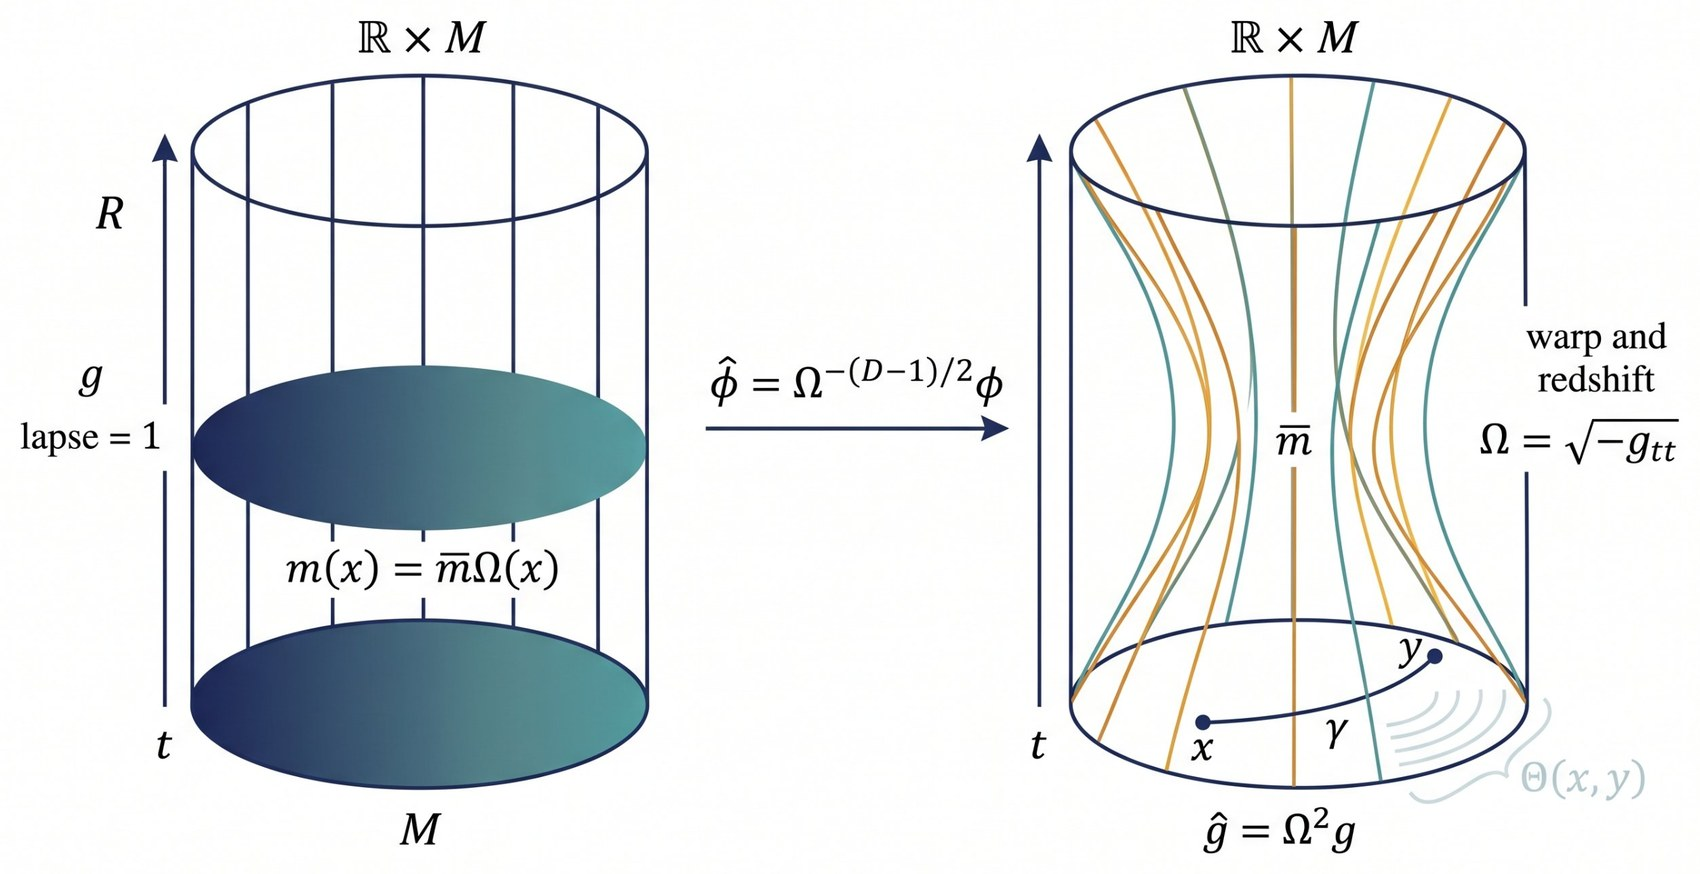
\includegraphics[width=0.84\textwidth]{figures/fig_lapse.jpg}
\caption{Proposition~\ref{prop:lapse}. Left: a field with the position-dependent gap $m(x)=\bar m\,\Omega(x)$ on the ultrastatic spacetime $\R\times\M$ with spatial metric $g$ and lapse one. Right: the same correlations are those of a field of constant mass $\bar m$ on the static spacetime with spatial metric $\hat g=\Omega^2g$ and lapse $\Omega=\sqrt{-g_{tt}}$. $\Theta(x,y)$ is the prefactor of Theorem~\ref{thm:vargap} along the geodesic $\gamma$. Schematic.}\label{fig:lapse}
\end{figure}


\begin{proof}
On a static spacetime with lapse $\Omega$ and spatial metric $\hat g$, $\Box=-\Omega^{-2}\partial_t^2+\Omega^{-1}\operatorname{div}_{\hat g}(\Omega\nabla_{\hat g}\,\cdot\,)$, so the Klein--Gordon equation reads $\partial_t^2\hat\phi=-\hat B\hat\phi$ with $\hat B=-\Omega\operatorname{div}_{\hat g}(\Omega\nabla_{\hat g}\,\cdot\,)+\Omega^2(\bar m^2+\mathcal V)$. We claim $\hat B=\Omega^{-a}A_g\Omega^{a}$. Indeed, with $\Delta_gu=\Omega^2[\Delta_{\hat g}u-(D-2)\langle\nabla\ln\Omega,\nabla u\rangle_{\hat g}]$ and $2a-(D-2)=1$,
\[
\Omega^{-a}\Delta_g(\Omega^{a}u)=\Omega^2\big[\Delta_{\hat g}u+\langle\nabla\ln\Omega,\nabla u\rangle_{\hat g}\big]+u\,\Omega^{-a}\Delta_g\Omega^{a}
=\Omega\operatorname{div}_{\hat g}(\Omega\nabla_{\hat g}u)-\Omega^2\mathcal V\,u .
\]
Thus $\phi=\Omega^{a}\hat\phi$ solves $\partial_t^2\phi=-A_g\phi$ if and only if $\hat\phi$ solves the static equation. The momentum conjugate to $\hat\phi$ with respect to $\dd V_{\hat g}$ is $\hat\pi=\Omega^{-1}\partial_t\hat\phi$, so $\int(\hat\phi_1\hat\pi_2-\hat\phi_2\hat\pi_1)\,\dd V_{\hat g}=\int\Omega^{-2a}(\phi_1\partial_t\phi_2-\phi_2\partial_t\phi_1)\,\Omega^{D-1}\dd V_g$, which is the symplectic form of the first system because $2a=D-1$. The ground state of a linear system with strictly positive generator is determined by the symplectic space and the time evolution, hence the two ground states correspond. The smearing functions follow from $\phi(f)=\int f\,\Omega^{a}\hat\phi\,\Omega^{-D}\dd V_{\hat g}$ and $\pi(f)=\int f\,\Omega^{a+1}\hat\pi\,\Omega^{-D}\dd V_{\hat g}$.
\end{proof}

In the spatial reading a position-dependent gap is thus the same as a gravitational redshift: $\Omega$ is the lapse $\sqrt{-g_{tt}}$ of a static spacetime whose spatial metric is $\hat g$ and whose optical metric is $g$. This is the only place in this paper where a component of a spacetime metric appears, and it is restricted to the static case.

The next theorem makes both readings quantitative. It rests on the observation that the equal-time correlator is a Euclidean Green function in one dimension more, so that Proposition~\ref{prop:weyl} applies with a \emph{single} metric.

\begin{theorem}[Correlators for a variable gap]\label{thm:vargap}
Let $A_g=-\Delta_g+\bar m^2\Omega^2$, $\hat g=\Omega^2g$ and $\hat r=d_{\hat g}(x,y)$.
\begin{enumerate}[label=\textup{(\alph*)}]
\item \emph{Euclidean reading.} Let $d=\dim\M$, $r_0<\mathrm{inj}(\M,\hat g)$, and let $\hat u_0,\hat u_1$ be the heat-kernel coefficients of $-\Delta_{\hat g}+\hat V$ on $(\M,\hat g)$. There are $m_0,C$ such that for $\bar m\ge m_0$ and $1/\bar m\le\hat r\le r_0$
\begin{equation}\label{eq:vargapE}
\Big|\frac{G_g(x,y)}{\chi(x)\chi(y)\,k_1^{\mathrm{flat}}(\hat r;\bar m)}-\hat u_0(x,y)-\frac{\hat r}{2\bar m}\,\rho_1(\bar m\hat r)\,\hat u_1(x,y)\Big|\le C\,\frac{\hat r^2}{\bar m^2}.
\end{equation}
\item \emph{Spatial reading.} Let $D=\dim\M$, $r_0<\mathrm{inj}(\M\times\R^3,\hat g+\Omega^2|\dd\tau|^2)$, and
\begin{equation}\label{eq:Theta}
\Theta(x,y)=\frac{\hat r}{\Omega(x)\,\Omega(y)\int_\gamma\Omega^{-2}\,\dd s_{\hat g}} ,
\end{equation}
where $\gamma$ is the minimising $\hat g$-geodesic from $x$ to $y$. There are $m_0,C$ such that for $\bar m\ge m_0$ and $1/\bar m\le\hat r\le r_0$ the correlators $X=\tfrac12A_g^{-1/2}$ and $P=\tfrac12A_g^{1/2}$ satisfy
\begin{equation}\label{eq:vargapS}
\begin{aligned}
\Big|\frac{X(x,y)}{(\Omega(x)\Omega(y))^{\frac{D-1}{2}}\,X^{\mathrm{flat}}_{\bar m}(\hat r)}-\hat u_0(x,y)\,\Theta(x,y)^{1/2}\Big|&\le C\,\frac{\hat r}{\bar m},\\
\Big|\frac{P(x,y)}{(\Omega(x)\Omega(y))^{\frac{D+1}{2}}\,P^{\mathrm{flat}}_{\bar m}(\hat r)}-\hat u_0(x,y)\,\Theta(x,y)^{3/2}\Big|&\le C\,\frac{\hat r}{\bar m},
\end{aligned}
\end{equation}
where $X^{\mathrm{flat}}_{\bar m},P^{\mathrm{flat}}_{\bar m}$ are the flat correlators of mass $\bar m$ in dimension $D$ and $\hat u_0$ is the Van Vleck factor of $(\M,\hat g)$.
\end{enumerate}
\end{theorem}

In terms of the two lengths $\hat d=\int_\gamma m\,\dd s_g=\bar m\hat r$ and $T=\int_\gamma\dd s_g/m$, with $m=\bar m\Omega$, one has $\Theta=\hat d/(m(x)m(y)T)$, and the first line of \eqref{eq:vargapS} reads, for $\bar m\hat r\gg1$,
\begin{equation}\label{eq:twolengths}
X(x,y)\simeq\frac{\big(m(x)m(y)\big)^{\frac{D-2}{2}}\;\hat u_0(x,y)\;e^{-\hat d}}{2\,(2\pi)^{D/2}\;\hat d^{\,\frac{D-1}{2}}\;T^{1/2}} ,
\end{equation}
which reduces to the flat formula of Appendix~\ref{app:decay} for constant $m$, where $T=r/m$.

\begin{proof}
(a) By Proposition~\ref{prop:weyl}(ii), $G_g=\chi(x)\chi(y)\hat G$ with $\hat G$ the Green function of $-\Delta_{\hat g}+\hat V+\bar m^2$. The operator $-\Delta_{\hat g}+\hat V$ is of Laplace type with a potential that does not depend on $\bar m$, the asymptotics \eqref{eq:strong} of \cite{Ludewig} hold for such operators, and the proof of Theorem~\ref{thm:curved} for $\sigma=1$ uses nothing else; the bound $p_s\le C$ for $s>1$ is replaced by $p_s\le Ce^{s\|\hat V\|_\infty}$, which is harmless for $\bar m^2\ge2\|\hat V\|_\infty$.

(b) \emph{Step 1.} For $j\in\{1,3\}$ let $G_j$ be the Green function of $-\Delta_{\R^j}+A_g=-\Delta_{g_j}+\bar m^2\Omega^2$ on $(\M\times\R^j,\,g_j=g+|\dd\tau|^2)$. Since $\int\frac{\dd\omega}{2\pi}(a+\omega^2)^{-1}=\tfrac12a^{-1/2}$, the spectral theorem gives $X(x,y)=G_1((x,0),(y,0))$. For $P$ we use $a^{1/2}=\tfrac1\pi\int_0^\infty\lambda^{-1/2}\big(1-\lambda(a+\lambda)^{-1}\big)\dd\lambda$ and $\int_{\R^3}\frac{\dd^3\omega}{(2\pi)^3}F(|\omega|^2)=\tfrac1{4\pi^2}\int_0^\infty\lambda^{1/2}F(\lambda)\,\dd\lambda$: off the diagonal the kernel of $A_g^{1/2}$ is $-\tfrac1\pi\int_0^\infty\lambda^{1/2}(A_g+\lambda)^{-1}(x,y)\,\dd\lambda$, hence
\[
P(x,y)=-2\pi\,G_3\big((x,0),(y,0)\big)\qquad(x\ne y).
\]

\emph{Step 2.} On $\M\times(S^1_\ell)^j$ the Green function is the sum over the images $\tau\mapsto\tau+\ell n$, $n\in\mathbb Z^j$. The image terms are kernels of functions of $A_g$ that are exponentially small: writing them as $A_g^{-k}\,F_n(A_g)\,A_g^{-k}$ with $k>D/4$ and $\|F_n(A_g)\|\le C\bar m^{4k+2}e^{-|n|\ell\bar m\Omega_{\min}/2}$, and using $\sup_x\|A_g^{-k}\delta_x\|\le C$, they are bounded by $C\bar m^{4k+2}e^{-\ell\bar m\Omega_{\min}/2}$. For $\ell$ fixed and large this is smaller than $e^{-2\bar mr_0}$, hence negligible against the error terms in \eqref{eq:vargapS}.

\emph{Step 3.} Apply (a) on the closed manifold $\M\times(S^1_\ell)^j$ of dimension $D+j$ with the metric $g_j$ and the function $\Omega(x)$. For $\ell$ large, $r_0$ is below its injectivity radius with respect to $\hat g_j=\hat g+\Omega^2|\dd\tau|^2$. The conformal factor is $\chi=\Omega^{(D+j-2)/2}$, and by \eqref{eq:kflat} the flat Green function in dimension $D+j$ is the flat correlator in dimension $D$: $k_1^{\mathrm{flat},D+1}=X^{\mathrm{flat}}$ and $-2\pi k_1^{\mathrm{flat},D+3}=P^{\mathrm{flat}}$.

\emph{Step 4.} The length of any curve in $(\M\times\R^j,\hat g_j)$ is at least the $\hat g$-length of its projection to $\M$, so $d_{\hat g_j}((x,0),(y,0))=d_{\hat g}(x,y)$, and $\gamma$, viewed in the slice $\tau=0$, is the minimising geodesic.

\emph{Step 5.} $\hat g_j$ is a warped product with base $(\M,\hat g)$, flat fibre and warping function $\Omega$. Along the horizontal geodesic $\gamma$ the Jacobi equation splits; the horizontal part is the Jacobi equation of $(\M,\hat g)$, and a vertical field $\varphi(s)E$, with $E$ a parallel unit vertical vector, satisfies $\varphi''=(f''/f)\varphi$ with $f(s)=\Omega(\gamma(s))$. The solution with $\varphi(0)=0$, $\varphi'(0)=1$ is $\varphi(s)=f(0)f(s)\int_0^sf^{-2}$. Hence the Jacobian of the exponential map of $\hat g_j$ is that of $\hat g$ times $(\varphi(\hat r)/\hat r)^j=\Theta^{-j}$, and the Van Vleck factor, its inverse square root, is $\hat u_0\,\Theta^{j/2}$. Since the coefficient $\hat u_1$ is bounded and $\hat u_0\Theta^{j/2}$ is bounded below, \eqref{eq:vargapE} gives \eqref{eq:vargapS}.
\end{proof}

The same argument with $j$ auxiliary dimensions gives the kernel of $A_g^{j/2-1}$ for every $j\ge1$. The potential $\hat V$ of the product is the static potential $\mathcal V$ of Proposition~\ref{prop:lapse}: the theorem is the statement that the ground-state correlator of a static spacetime is its Euclidean Green function, expanded around the totally geodesic slice. Three consequences follow.

\emph{(i)} In both readings the exponential decay is governed by $d_{\hat g}$. For classical correlations (Proposition~\ref{prop:classical}) the data therefore satisfy the profile assumption with respect to $\hat g$, up to the node factors $\chi(x_i)\chi(x_j)$ and corrections of the kind treated in Theorem~\ref{thm:window}.

\emph{(ii)} In the spatial reading the power-law prefactor contains a second length, $T$, weighted with $\Omega^{-1}$ where $\hat d$ is weighted with $\Omega$. It is the Van Vleck factor in the Euclidean time direction: the rate at which geodesics of the static spacetime that start on the slice spread in time. The lapse is thus visible in the correlations already at leading power-law order, and not only at curvature order as in the Euclidean reading; singling out a time direction breaks the Weyl equivalence of Proposition~\ref{prop:weyl}.

\emph{(iii)} For the reconstruction this means that a variable gap shifts the surprisal distance by $\xi_0\cdot O(\ln(\Omega_{\max}/\Omega_{\min}))$, so $\hat g$ is recovered without distortion only for $\xi_0\ll\xi$.

A one-dimensional numerical check of \eqref{eq:vargapS} is in Appendix~\ref{app:num}.

\emph{(iv) What is independent of the nodes.} Measured correlators carry unknown node factors, $x_{ab}=F_aF_bX(a,b)$, and so does the mutual information when the nodes are not identical. Cross-ratios such as $x_{ad}x_{bc}/(x_{ac}x_{bd})$ do not. In one dimension they can be evaluated in closed form.

\begin{proposition}[Lapse from cross-ratios, $D=1$]\label{prop:crossratio}
Let $D=1$, $\mathfrak D(x)=\int^xm\,\dd s$ and $\mathfrak W(x)=\int^x\dd s/m$. For points $a<b<c<d$ within the range of Theorem~\ref{thm:vargap} and to leading order in $1/\bar m\hat r$,
\begin{equation}
\begin{aligned}
\frac{X_{ad}X_{bc}}{X_{ac}X_{bd}}&=\Big[\frac{(\mathfrak W_c-\mathfrak W_a)(\mathfrak W_d-\mathfrak W_b)}{(\mathfrak W_d-\mathfrak W_a)(\mathfrak W_c-\mathfrak W_b)}\Big]^{1/2},\\
\frac{X_{ab}X_{cd}}{X_{ac}X_{bd}}&=e^{2(\mathfrak D_c-\mathfrak D_b)}\Big[\frac{(\mathfrak W_c-\mathfrak W_a)(\mathfrak W_d-\mathfrak W_b)}{(\mathfrak W_b-\mathfrak W_a)(\mathfrak W_d-\mathfrak W_c)}\Big]^{1/2}.
\end{aligned}
\end{equation}
Consequently the node-independent data determine $\mathfrak D$ up to an additive constant and $\mathfrak W$ up to a M\"obius transformation, and the gap $m=(\dd\mathfrak D/\dd\mathfrak W)^{1/2}$ up to the two-parameter family $m\mapsto m\,|\gamma\mathfrak W+\delta|$; all members of the family give the same cross-ratios.
\end{proposition}

\begin{proof}
For $D=1$, \eqref{eq:twolengths} is $X(x,y)\simeq e^{-(\mathfrak D_y-\mathfrak D_x)}\big(8\pi\,m(x)m(y)(\mathfrak W_y-\mathfrak W_x)\big)^{-1/2}$. In both ratios the factors $m(\cdot)$ cancel; in the first the exponentials cancel as well. The first ratio is the square root of a projective cross-ratio of the four numbers $\mathfrak W_a,\dots,\mathfrak W_d$, and cross-ratios determine a function up to M\"obius transformations and are invariant under them. Given $\mathfrak W$, the second ratio gives the differences of $\mathfrak D$. Under $\tilde{\mathfrak W}=(\alpha\mathfrak W+\beta)/(\gamma\mathfrak W+\delta)$ with $\alpha\delta-\beta\gamma=1$ one has $\dd\tilde{\mathfrak W}=\dd\mathfrak W/(\gamma\mathfrak W+\delta)^2$, hence $\tilde m=m|\gamma\mathfrak W+\delta|$.
\end{proof}

So the lapse can be read off from the correlations without knowledge of the nodes, up to a constant factor ($\delta$) and one further parameter ($\gamma$), which reflects the projective symmetry of the one-dimensional problem. In higher dimensions the same ambiguity is possible only for special geometries.

\begin{proposition}[Rigidity for $D\ge2$]\label{prop:rigid}
Let $\varpi=\Omega^{-2}$ and $T(x,y)=\int_\gamma\varpi\,\dd s_{\hat g}$ along minimising $\hat g$-geodesics. Suppose a second positive function $\tilde\varpi$ and a positive function $b$ satisfy $\tilde T(x,y)=b(x)b(y)T(x,y)$ for all sufficiently close $x,y$. Then $u=1/b$ solves
\begin{equation}\label{eq:rigid}
\operatorname{Hess}_{\hat g}u=\tfrac12\big(\dd u\otimes\dd\ln\varpi+\dd\ln\varpi\otimes\dd u\big).
\end{equation}
In particular, if $u$ is not constant, its regular level sets are totally geodesic hypersurfaces of $(\M,\hat g)$.
\end{proposition}

\begin{proof}
Let $y=\exp_x(rv)$ with $|v|=1$ and write $\partial_v^k$ for derivatives along the geodesic. Then $T=\varpi r+\tfrac12\partial_v\varpi\,r^2+\tfrac16\partial_v^2\varpi\,r^3+O(r^4)$, and the same for $\tilde T$. Order $r$ gives $\tilde\varpi=b^2\varpi$, order $r^2$ is then satisfied identically, and order $r^3$ gives $b\varpi\,\partial_v^2b-b\,\partial_vb\,\partial_v\varpi-2\varpi(\partial_vb)^2=0$ for all $v$. With $u=1/b$ this is $\partial_v^2u=\partial_vu\,\partial_v\ln\varpi$, which is \eqref{eq:rigid} evaluated on $(v,v)$. For $v$ tangent to a level set of $u$ the right-hand side vanishes, so the second fundamental form of the level set is zero.
\end{proof}

For $D=1$, \eqref{eq:rigid} is solved exactly by the M\"obius family of Proposition~\ref{prop:crossratio}. For $D\ge2$ a foliation by totally geodesic hypersurfaces does not exist for a generic metric, so generically $b$ is constant and the lapse is determined up to a constant factor by the node-independent data. An example of the exceptional case is a lapse that depends on one coordinate of a flat $\hat g$.

\begin{proposition}[No independent dynamics]\label{prop:conformal}
Let $d\ge3$, $\hat g=\Omega^2g$ and $\chi=\Omega^{(d-2)/2}$. Then
\begin{equation}
\int\sqrt{\hat g}\,R_{\hat g}\,\dd^dx=\int\sqrt g\,\Big[\chi^2R_g+\frac{4(d-1)}{d-2}\,|\nabla\chi|_g^2\Big]\dd^dx,\qquad \Vol(\hat g)=\int\sqrt g\,\chi^{\frac{2d}{d-2}}\,\dd^dx .
\end{equation}
For $d=4$ the first integrand is $\Omega^2R_g+6|\nabla\Omega|^2$.
\end{proposition}

\begin{proof}
$R_{\hat g}=\Omega^{-2}[R_g-2(d-1)\Delta_g\ln\Omega-(d-2)(d-1)|\nabla\ln\Omega|^2]$ and $\sqrt{\hat g}=\Omega^d\sqrt g$. Integrating the middle term by parts gives $\int\sqrt g\,\Omega^{d-2}[R_g+(d-1)(d-2)|\nabla\ln\Omega|^2]$, and $|\nabla\chi|^2=\tfrac{(d-2)^2}{4}\Omega^{d-2}|\nabla\ln\Omega|^2$.
\end{proof}

Every functional of the reconstructed metric $\hat g$, in particular the heat-trace coefficients of Corollary~\ref{cor:curv} and the induced action of Remark~\ref{rem:induced}, is a functional of $(g,\Omega)$ in which $\Omega$ appears as the conformal mode. In a Euclidean action $-\tfrac12M^2\int\sqrt{\hat g}R_{\hat g}$ its kinetic term has the sign opposite to that of an ordinary scalar; this is the well-known conformal-factor instability and not a new feature. The picture is therefore coherent but modest: the additional scalar in $C_{ij}$ is the conformal factor of the metric (Euclidean reading) or the lapse of a static spacetime (spatial reading). It is not a matter field and not an independent dilaton; the dilaton of \cite{CC06} becomes an independent field only if a second, reference metric is given, which the correlation data do not supply.

\section{Time-odd correlations and extrinsic curvature}\label{sec:time}

The mutual information of an equal-time state is invariant under time reversal, whereas the extrinsic curvature of the slice is odd. This section shows where the extrinsic curvature is stored and why entropic quantities cannot see its sign. We consider the field on a spacetime with unit lapse and a shift,
\begin{equation}
\dd s^2=-\dd t^2+h_{ij}(\dd x^i-\beta^i\dd t)(\dd x^j-\beta^j\dd t),\qquad n=\partial_t+\beta\cdot\nabla,\qquad K_{ij}=\tfrac12(\mathcal L_nh)_{ij},
\end{equation}
so that $K_{ij}=\nabla_{(i}\beta_{j)}$ in the stationary case. With $\pi=n\phi$, $A=-\Delta_h+m^2$ and $B=\beta\cdot\nabla$ acting on scalars,
\begin{equation}\label{eq:Hshift}
H=\tfrac12(\pi,\pi)+\tfrac12(\phi,A\phi)-(\pi,B\phi),\qquad\dot\phi=\pi-B\phi,\qquad\dot\pi=-A\phi+B^{T}\pi ,
\end{equation}
where the transpose refers to $L^2(\dd V_h)$. A Gaussian state is described by $X=\langle\phi\phi\rangle$, $P=\langle\pi\pi\rangle$ and the time-odd correlator $Y(x,y)=\tfrac12\langle\{\phi(x),\pi(y)\}\rangle$.

\begin{proposition}[Kinematic identity]\label{prop:kin}
For every state and every time,
\begin{equation}\label{eq:kin}
\partial_tX+\mathcal L_\beta X=Y+Y^{T},\qquad(\mathcal L_\beta X)(x,y)=\big(\beta(x)\cdot\nabla_x+\beta(y)\cdot\nabla_y\big)X(x,y).
\end{equation}
With a lapse $\Omega$, that is, $n=\Omega^{-1}(\partial_t+\beta\cdot\nabla)$ and $\pi=n\phi$, the right-hand side is $\Omega(x)Y(y,x)+\Omega(y)Y(x,y)$.
\end{proposition}

\begin{proof}
$\partial_t\langle\phi(x)\phi(y)\rangle=\langle\dot\phi(x)\phi(y)+\phi(x)\dot\phi(y)\rangle$ with $\dot\phi=\Omega\pi-\beta\cdot\nabla\phi$.
\end{proof}

The left-hand side is the derivative of the correlator along the normal flow. Since the reconstruction of Section~\ref{sec:recon} maps $X$ to the metric, \eqref{eq:kin} is the counterpart of $K=\tfrac12\mathcal L_nh$ at the level of correlations: the symmetric part of $Y$ is the velocity of the correlation geometry. The identity yields the extrinsic curvature without any asymptotic analysis of $Y$.

\begin{theorem}[X-ray form]\label{thm:xray}
Let $Y^{\mathrm s}(x,y)=\tfrac12(Y(x,y)+Y(y,x))$.
\begin{enumerate}[label=\textup{(\alph*)}]
\item Let $h$ be flat, $\Omega=1$, and consider the ground state of \eqref{eq:Hshift} to first order in an arbitrary smooth shift $\beta$. Then, with $v=y-x$ and $r=|v|$,
\begin{equation}\label{eq:xray}
Y^{\mathrm s}(x,y)=\tfrac12\,P^{\mathrm{flat}}(r)\int_0^1K_{x+sv}(v,v)\,\dd s .
\end{equation}
\item In general, if at some time the correlator has the profile form $X_t(x,y)=F(d_{h_t}(x,y))$ on a set of pairs, with $F$ independent of $t$, then on this set
\begin{equation}\label{eq:xraygen}
\Omega(x)Y(y,x)+\Omega(y)Y(x,y)=F'(d_h(x,y))\int_\gamma\Omega\,K(\dot\gamma,\dot\gamma)\,\dd s ,
\end{equation}
where $\gamma$ is the unit-speed minimising geodesic from $x$ to $y$.
\end{enumerate}
\end{theorem}

\begin{figure}[t]
\centering
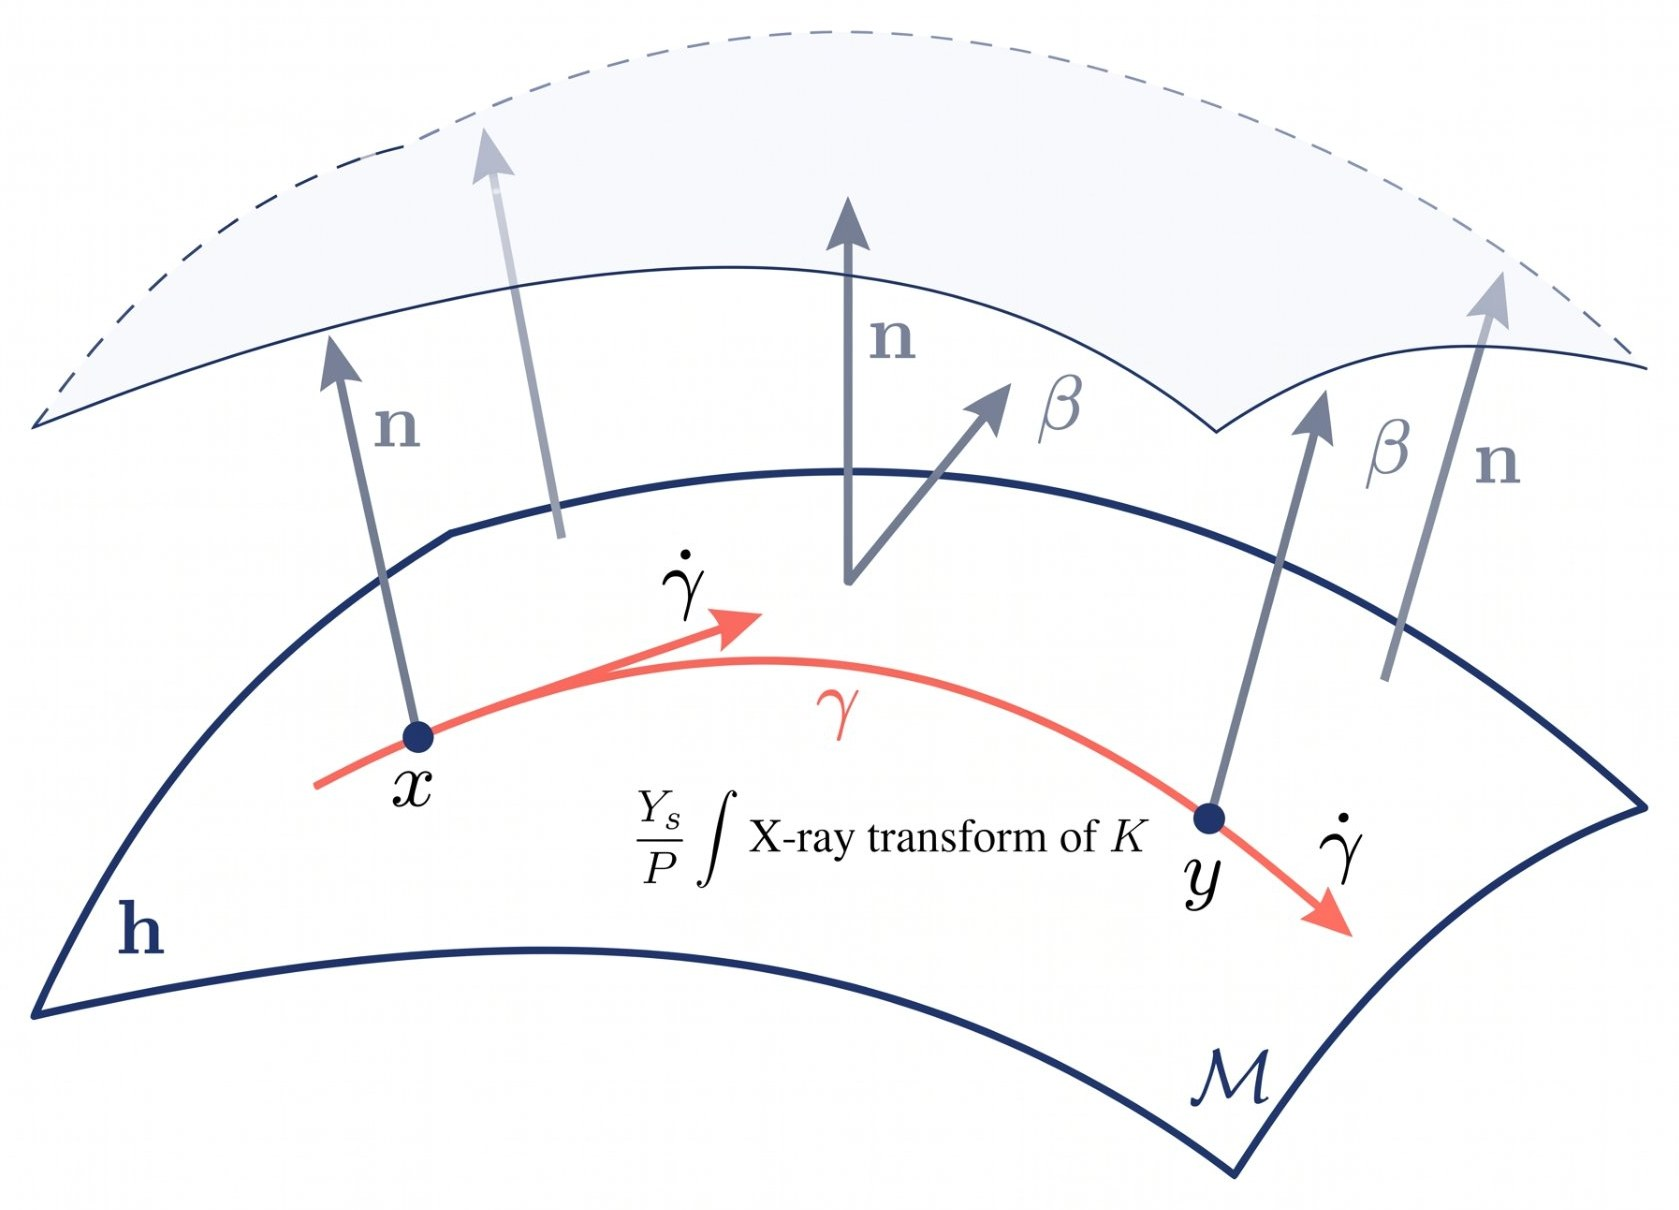
\includegraphics[width=0.72\textwidth]{figures/fig_xray.jpg}
\caption{Theorem~\ref{thm:xray}. A slice with metric $h$, unit normal $n$ and shift $\beta$. The symmetric part $Y^{\mathrm s}$ of the time-odd correlator of two points $x,y$ is given by the integral of $K(\dot\gamma,\dot\gamma)$ along the geodesic $\gamma$ joining them; in the flat case \eqref{eq:xray}, $2Y^{\mathrm s}/P$ is the mean of $K(v,v)$ along the segment. Schematic; the formula printed in the picture is shorthand for \eqref{eq:xray}.}\label{fig:xray}
\end{figure}


\begin{proof}
(b) By Proposition~\ref{prop:kin} the left-hand side is $(\partial_t+\mathcal L_\beta)F(d_{h_t}(x,y))=F'(d)\,(\partial_t+\mathcal L_\beta)d_{h_t}(x,y)$. The operator $\partial_t+\mathcal L_\beta$ differentiates along the flow of $\Omega n$, under which $h$ changes at the rate $\mathcal L_{\Omega n}h=2\Omega K$ on spatial vectors; the first variation of arc length gives $(\partial_t+\mathcal L_\beta)d_h(x,y)=\tfrac12\int_\gamma(2\Omega K)(\dot\gamma,\dot\gamma)\,\dd s$. (a) In first-order perturbation theory $\langle a_ka_l\rangle$ is purely imaginary (see the proof of Theorem~\ref{thm:YP}), so $X=X^{\mathrm{flat}}+O(\beta^2)$, and the state is stationary. Apply (b) with $F=X^{\mathrm{flat}}$, $F'(r)=rP^{\mathrm{flat}}(r)$ by \eqref{eq:kflat}, and $\int_\gamma K(\dot\gamma,\dot\gamma)\,\dd s=r^{-1}\int_0^1K_{x+sv}(v,v)\,\dd s$.
\end{proof}

Thus the symmetric part of the time-odd correlator, divided by $P$, is the X-ray transform of the extrinsic curvature: $2Y^{\mathrm s}/P$ is the mean of $K(v,v)$ along the segment, exactly and for an arbitrary shift in case (a). The ratio is independent of node factors, of the mass and of the surprisal distance. Part (b) covers curved slices, a lapse and non-stationary states at the order at which the correlator is a fixed profile of the instantaneous distance; in the situation of Theorem~\ref{thm:curved} the corrections come from the time dependence of $u_0$ and $u_1$ and are of relative order $r^2/\Lcurv^2$.

For the antisymmetric part and for the full correlator we have the following explicit result.

\begin{theorem}[Homogeneous deformation]\label{thm:YP}
Let $h$ be flat, and consider the ground state of \eqref{eq:Hshift} to first order in $\beta$. In the eigenbasis of $A$, with $\omega=\sqrt A$,
\begin{equation}\label{eq:Ymodes}
Y_{kl}=\frac{B_{kl}+B_{lk}\,\omega_l/\omega_k}{2(\omega_k+\omega_l)},\qquad\text{equivalently}\qquad2\omega(\omega Y+Y\omega)=\omega B+B^{T}\omega .
\end{equation}
For a linear shift $\beta(x)=Kx$ on $\R^D$, with a constant symmetric matrix $K$, the solution is, with $v=y-x$,
\begin{equation}\label{eq:YP}
Y(x,y)=\tfrac12\,K_{ij}v^iv^j\,P^{\mathrm{flat}}(|v|),\qquad\text{hence}\qquad\frac{Y}{X}=-\tfrac12\,m\,r\,K_{ij}n^in^j\,\big(1+O(1/mr)\big).
\end{equation}
\end{theorem}

\begin{proof}
With $\phi_l=(a_l+a_l^\dagger)/\sqrt{2\omega_l}$ and $\pi_k=-i\sqrt{\omega_k/2}\,(a_k-a_k^\dagger)$, the two-particle component of $V|0\rangle$ for $V=-(\pi,B\phi)$ is $-\tfrac i2\sum B_{kl}\sqrt{\omega_k/\omega_l}\,a_k^\dagger a_l^\dagger|0\rangle$, so first-order perturbation theory gives $\langle a_ka_l\rangle=ic_{kl}$ with $c_{kl}=\tfrac12[B_{kl}\sqrt{\omega_k/\omega_l}+B_{lk}\sqrt{\omega_l/\omega_k}]/(\omega_k+\omega_l)$, and $Y_{kl}=\sqrt{\omega_l/\omega_k}\,c_{kl}$. This is \eqref{eq:Ymodes}. For $\beta=Kx$ we have $B^{T}=-B-\operatorname{tr}K$ and, since $x_j$ acts as $i\partial_{\xi_j}$ in Fourier space, $[\omega,B]=K_{ij}\xi_i\xi_j/\omega$ is a Fourier multiplier. Hence $\omega B+B^{T}\omega=[\omega,B]-\omega\operatorname{tr}K$ and $Y$ is the multiplier $K_{ij}\xi_i\xi_j/4\omega^3-\operatorname{tr}K/4\omega$, that is,
\[
Y(x,y)=-\tfrac14K^{ij}\partial_i\partial_jk^{\mathrm{flat}}_{3/2}(r)-\tfrac14\operatorname{tr}K\,k^{\mathrm{flat}}_{1/2}(r).
\]
By \eqref{eq:kflat}, $\tfrac{\dd}{\dd r}k^{\mathrm{flat}}_{3/2}=-r\,k^{\mathrm{flat}}_{1/2}$ and $\tfrac{\dd}{\dd r}k^{\mathrm{flat}}_{1/2}=r\,k^{\mathrm{flat}}_{-1/2}$. Therefore $\partial_i\partial_jk_{3/2}=-n_in_j\,r^2k_{-1/2}-\delta_{ij}k_{1/2}$, the trace terms cancel, and $Y=\tfrac14K(n,n)\,r^2k^{\mathrm{flat}}_{-1/2}=\tfrac12K(v,v)P^{\mathrm{flat}}$. The ratio follows from $P/X=-(m/r)(1+O(1/mr))$.
\end{proof}

For a homogeneous deformation $Y$ is symmetric and \eqref{eq:YP} agrees with \eqref{eq:xray}. The extrinsic curvature in direction $n$ can be read off from pair data as $K(n,n)=2Y^{\mathrm s}/(r^2P)$ for short segments; a Killing shift gives $Y^{\mathrm s}=0$.

\emph{Non-stationary example.} On a spatially flat Friedmann spacetime $-\dd t^2+a(t)^2\dd x^2$ the modes are $\chi_k(t)e^{ikx}$ with $\chi_k=(2a^DW_k)^{-1/2}e^{-i\int W_k}$ and $W_k=\omega_p$ up to second adiabatic order, $\omega_p^2=p^2+m^2$, $p=k/a$. Hence $Y_p/X_p=\tfrac12\partial_t\ln|\chi_k|^2=-\tfrac12H\,(D-p^2/\omega_p^2)$ with $H=\dot a/a$, and the Fourier transform in the physical separation $v$ is $Y=-\tfrac{DH}{2}X-\tfrac H4\Delta_vk^{\mathrm{flat}}_{3/2}=\tfrac12H\,r^2P^{\mathrm{flat}}(r)$, which is \eqref{eq:YP} with $K_{ij}=H\delta_{ij}$. The Hubble rate of an expanding universe is therefore stored in the time-odd correlator of an adiabatic state, in agreement with Theorem~\ref{thm:xray}(b), although the spatial metric at a fixed time is flat.

\emph{A graph estimator.} Let $\zeta_{ij}=2Y^{\mathrm s}(x_i,x_j)/P(x_i,x_j)$ for $i\ne j$, where $P$ here denotes the momentum correlator, and let $P_{ij}$ be the transition matrix of Section~\ref{sec:setting}. With $c_4=\tfrac1{m_0}\int h(|u|)u_1^2u_2^2\,\dd u$ define
\begin{equation}
\kappa_N(i)=\frac{1}{c_h\xi^2}\sum_jP_{ij}\zeta_{ij},\qquad
\Gamma^K_N(f,g)(i)=\frac{1}{c_4\xi^4}\sum_jP_{ij}\,\zeta_{ij}\,(f_j-f_i)(g_j-g_i),
\end{equation}
and let $\Gamma_N(f,g)(i)=\frac{1}{c_h\xi^2}\sum_jP_{ij}(f_j-f_i)(g_j-g_i)$ be the usual carr\'e du champ.

\begin{proposition}[Consistency of the estimator]\label{prop:Kgraph}
In the situation of Theorem~\ref{thm:xray}(a) and under Assumption~\ref{ass:profile} for the flat metric, let $f,g\in C^3(\M)$ and $N\xi^{d}\ge C\log N$. Then with probability at least $1-CN^{-2}$, uniformly in $i$,
\begin{equation}
\kappa_N(i)=\operatorname{tr}K(x_i)+O(\varrho_N),\qquad
\tfrac12\big[\Gamma^K_N(f,g)-\kappa_N\,\Gamma_N(f,g)\big](i)=K(\nabla f,\nabla g)(x_i)+O(\varrho_N),
\end{equation}
with $\varrho_N=\xi+\sqrt{\log N/(N\xi^d)}$.
\end{proposition}

\begin{proof}
Fix $i$, write $x=x_i$ and $v=x_j-x$, and let $\delta'=\sqrt{\log N/(N\xi^d)}$. By \eqref{eq:xray} and Taylor's formula, $\zeta_{ij}=K_x(v,v)+\tfrac12(\partial_vK)_x(v,v)+O(|v|^4)$, in particular $|\zeta_{ij}|\le C|v|^2$. As in the proof of Lemma~\ref{lem:pointwise}, write $\sum_jP_{ij}\zeta_{ij}\,\Phi_{ij}=\mathcal N_i/\mathcal D_i$ with $\mathcal N_i=\frac1N\sum_jK_{ij}\zeta_{ij}\Phi_{ij}/q_j$, where $\Phi_{ij}$ is $1$ or $(f_j-f_i)(g_j-g_i)$. Replacing $q_j$ by $q_\xi(x_j)$ costs a relative error $O(\delta')$. The summands are then independent given $x_i$, bounded by $C\xi^{p-d}$ with variance at most $C\xi^{2p-d}$, where $p=2$ or $p=4$, so Bernstein's inequality and a union bound give $\mathcal N_i=\mathcal N_\xi(x)+O(\xi^p\delta')$ with probability $1-CN^{-2}$, and $\mathcal D_i=1+O(\xi^2+\delta')$. In the population integral $\mathcal N_\xi(x)=\int K_\xi(x,y)\zeta(x,y)\Phi(x,y)\mu(y)q_\xi(y)^{-1}\dd V(y)$ we substitute $y=x+\xi u$ and use $\mu/q_\xi=(m_0\xi^d)^{-1}(1+O(\xi^2))$ with bounded derivatives. The terms that are odd in $u$ vanish, so for $\Phi=1$
\[
\mathcal N_\xi(x)=\frac{\xi^2}{m_0}\int h(|u|)K_x(u,u)\,\dd u+O(\xi^4)=c_h\xi^2\operatorname{tr}K(x)+O(\xi^4),
\]
and for $\Phi=(f(y)-f(x))(g(y)-g(x))=\xi^2\partial_\alpha f\,\partial_\beta g\,u^\alpha u^\beta+O(\xi^3|u|^3)$, with the cubic term odd,
\[
\mathcal N_\xi(x)=\frac{\xi^4}{m_0}K_{\gamma\delta}\,\partial_\alpha f\,\partial_\beta g\int h(|u|)u^\alpha u^\beta u^\gamma u^\delta\,\dd u+O(\xi^6).
\]
By isotropy $\tfrac1{m_0}\int h\,u^\alpha u^\beta u^\gamma u^\delta=c_4(\delta^{\alpha\beta}\delta^{\gamma\delta}+\delta^{\alpha\gamma}\delta^{\beta\delta}+\delta^{\alpha\delta}\delta^{\beta\gamma})$, and the contraction is $\operatorname{tr}K\,\langle\dd f,\dd g\rangle+2K(\nabla f,\nabla g)$. Dividing by $c_h\xi^2$ and $c_4\xi^4$ and using $\Gamma_N(f,g)=\langle\dd f,\dd g\rangle+O(\xi^2+\delta')$, which follows in the same way, gives the claim; the bias is in fact $O(\xi^2)$.
\end{proof}

Evaluated on the embedding coordinates $\varphi_a$ this gives all components of $K$ in the spectral frame.

\emph{Inversion on the graph.} The short-segment estimator is not the only use of the data. In the situation of Theorem~\ref{thm:xray}(a), $\int_0^1K_{x+sv}(v,v)\,\dd s=(\beta(y)-\beta(x))\cdot(y-x)$, so that
\begin{equation}\label{eq:ddot}
\zeta_{ij}=\tfrac12\,\partial_n\big(d_h(x_i,x_j)^2\big):
\end{equation}
the time-odd data are the normal derivative of the matrix of squared distances. Inverting the X-ray transform on the graph is therefore the same as differentiating the reconstruction pipeline: with $\dot d_{ij}=\zeta_{ij}/d_{ij}$ and $\dot K_{ij}=h'(d_{ij}/\xi)\,\dot d_{ij}/\xi$ one obtains $\dot W$, $\dot{\Lc}$ and the derivative of every reconstructed quantity, for instance $-\tfrac12\tfrac{\dd}{\dd\tau}\Gamma_N(f,g)\to K(\nabla f,\nabla g)$, since $\partial_nh^{ab}=-2K^{ab}$. This uses all pairs within the kernel range and has no $O(|v|^3)$ error. In flat space \eqref{eq:ddot} is also the linear system of infinitesimal rigidity for the velocity field $\beta$ at the nodes, which is solvable up to Killing fields. At the population level the differentiated pipeline converges.

\begin{proposition}[Differentiated pipeline]\label{prop:dotL}
Let $h_\tau$, $|\tau|\le\tau_0$, be a smooth family of metrics on $\M$ with $\partial_\tau h_\tau=2K_\tau$, let the profile be twice continuously differentiable with $|h^{(j)}(s)|\le Ae^{-s}$ for $j\le2$, and let $\Lc^\tau_\xi=\tfrac{2}{c_h\xi^2}(1-P^\tau_\xi)$ be the population operator of Theorem~\ref{thm:LB} for the kernel $h(d_{h_\tau}(x,y)/\xi)$. Then for $f\in C^6(\M)$, uniformly on $\M$ and in $\tau$,
\begin{equation}
\partial_\tau\big(\Lc^\tau_\xi f\big)=2K^{ab}\nabla_a\nabla_bf+\big(2\nabla_aK^{ab}-\nabla^b\operatorname{tr}K\big)\partial_bf+O(\xi),
\end{equation}
where the right-hand side is $-\partial_\tau(\Delta_{h_\tau}f)$.
\end{proposition}

\begin{proof}
Let $G_\xi(\tau)=\Lc^\tau_\xi f+\Delta_{h_\tau}f$. The constants in Appendix~\ref{app:LB} depend only on bounds for the curvature, the injectivity radius and the density, which are uniform for $|\tau|\le\tau_0$; hence $|G_\xi(\tau)|\le C\xi^2$. We claim $|\partial_\tau^2G_\xi|\le C$. The derivatives $\partial_\tau^l$, $l\le2$, of the kernel are sums of terms $h^{(j)}(d_\tau/\xi)$ times polynomials in $\partial_\tau^ld_\tau/\xi$, and $\partial_\tau^ld_\tau=d_\tau\,b_l$ with $b_l$ bounded and smooth off the diagonal. In the variable $u=\exp_x^{-1}(y)/\xi$ these are kernels $\kappa(x,u)$ with the same decay as $h$ which are even in $u$ up to relative corrections $O(\xi|u|)$, because $d_\tau(x,\exp_x(\xi u))^2=\xi^2h_\tau(u,u)+O(\xi^3|u|^3)$. For such kernels $\int\kappa\,(f(y)-f(x))\,\rho(y)\,\dd V(y)=O(\xi^{d+2})$ for every smooth $\rho$, since the term of order $\xi^{d+1}$ is the integral of an odd function; this is the mechanism of Lemma~\ref{lem:G}. Applying it to the numerator of $P^\tau_\xi f-f$ and its derivatives, and noting that the denominator and its derivatives are of order one, gives $\partial_\tau^2(\Lc^\tau_\xi f)=O(1)$. By the Landau inequality $\|G'\|_\infty\le2(\|G\|_\infty\|G''\|_\infty)^{1/2}$ on an interval, $|\partial_\tau G_\xi|\le C\xi$. The formula for $\partial_\tau\Delta_{h_\tau}$ is the first variation of the Laplacian under $\delta h=2K$.
\end{proof}

In terms of the data, $\partial_\tau$ of the kernel is $h'(d_{ij}/\xi)\,\zeta_{ij}/(\xi d_{ij})$. The corresponding statement for the $N$-point operator, with a sampling error as in Lemma~\ref{lem:pointwise}, is expected but not proven. The construction follows a suggestion made to us in the course of this work; the present form uses the exact ratio $Y^{\mathrm s}/P$ and therefore needs neither the mass nor the surprisal distance.

\begin{proposition}[No time-odd local invariant]\label{prop:Todd}
Every function of a two-mode Gaussian state that is invariant under local symplectic transformations is invariant under time reversal $(\phi,\pi)\mapsto(\phi,-\pi)$. In particular the mutual information, the logarithmic negativity and all R\'enyi quantities are even functions of $Y$.
\end{proposition}

\begin{proof}
By local symplectic transformations every two-mode covariance matrix can be brought to the standard form $\sigma_A=a\mathbf 1$, $\sigma_B=b\mathbf 1$, $\sigma_{AB}=\operatorname{diag}(c_+,c_-)$, and $(a,b,c_+,c_-)$ is a complete set of invariants \cite{Simon,DGCZ}. Time reversal acts on each block by conjugation with $\operatorname{diag}(1,-1)$ and leaves the standard form unchanged.
\end{proof}

Thus $C_{ij}$ determines $K$ at best to second order and without its sign. The sign requires a \emph{polarisation}: the specification, at each node, of which quadrature is the configuration variable, equivalently the identification $\pi=n\phi$. This structure is kinematical, part of the canonical commutation relations together with the dynamics, and not entropic. The same structure carries the causal cones: for $\partial_t^2\phi=-A\phi$ the commutator function $\sin(t\sqrt A)/\sqrt A$ is supported in $\{d_g\le|t|\}$ by finite propagation speed, with $g$ the optical metric, while the state determines $\hat g$ (Theorem~\ref{thm:vargap}). That causal cones together with a conformal factor, read off from the correlators of a field, determine the metric is the starting point of \cite{SAK,Kempf21,PercheMM}. In this sense a static Lorentzian metric is encoded in the pair (state, algebra with dynamics), and the Lorentzian signature is the hyperbolicity that follows from the symplectic form and the positivity of $H$; the commutative Gaussian measure of the Euclidean reading has no cones.

\subsection{Time without an external Hamiltonian}\label{sec:modular}

So far the Hamiltonian was given. For states of the vacuum type it need not be: the generator of time translations is contained in the state together with the net of local algebras. The basis is the theorem of Bisognano and Wichmann and its abstract converse.

\begin{proposition}[Dynamics from modular data; cited results]\label{prop:modular}
\textup{(i)} In the vacuum of a quantum field theory satisfying the Wightman axioms, the modular Hamiltonian of the half-space $\{x_1>a\}$ is $K_a=2\pi\int_{x_1>a}(x_1-a)\,T_{00}\,\dd^Dx$, the generator of boosts \cite{BW}. Hence
\begin{equation}\label{eq:HfromK}
H_{\{x_1>a\}}\equiv\int_{x_1>a}T_{00}\,\dd^Dx=-\frac1{2\pi}\,\frac{\partial K_a}{\partial a}.
\end{equation}
\textup{(ii)} Conversely, let $\mathcal N\subset\mathcal M$ be von Neumann algebras with a common cyclic and separating vector such that the modular group of $\mathcal M$ maps $\mathcal N$ into itself for $t\le0$. Then there is a one-parameter unitary group with positive generator that translates $\mathcal M$ onto $\mathcal N$ \cite{Borchers,Wiesbrock,ArakiZsido}.
\end{proposition}

\begin{figure}[t]
\centering
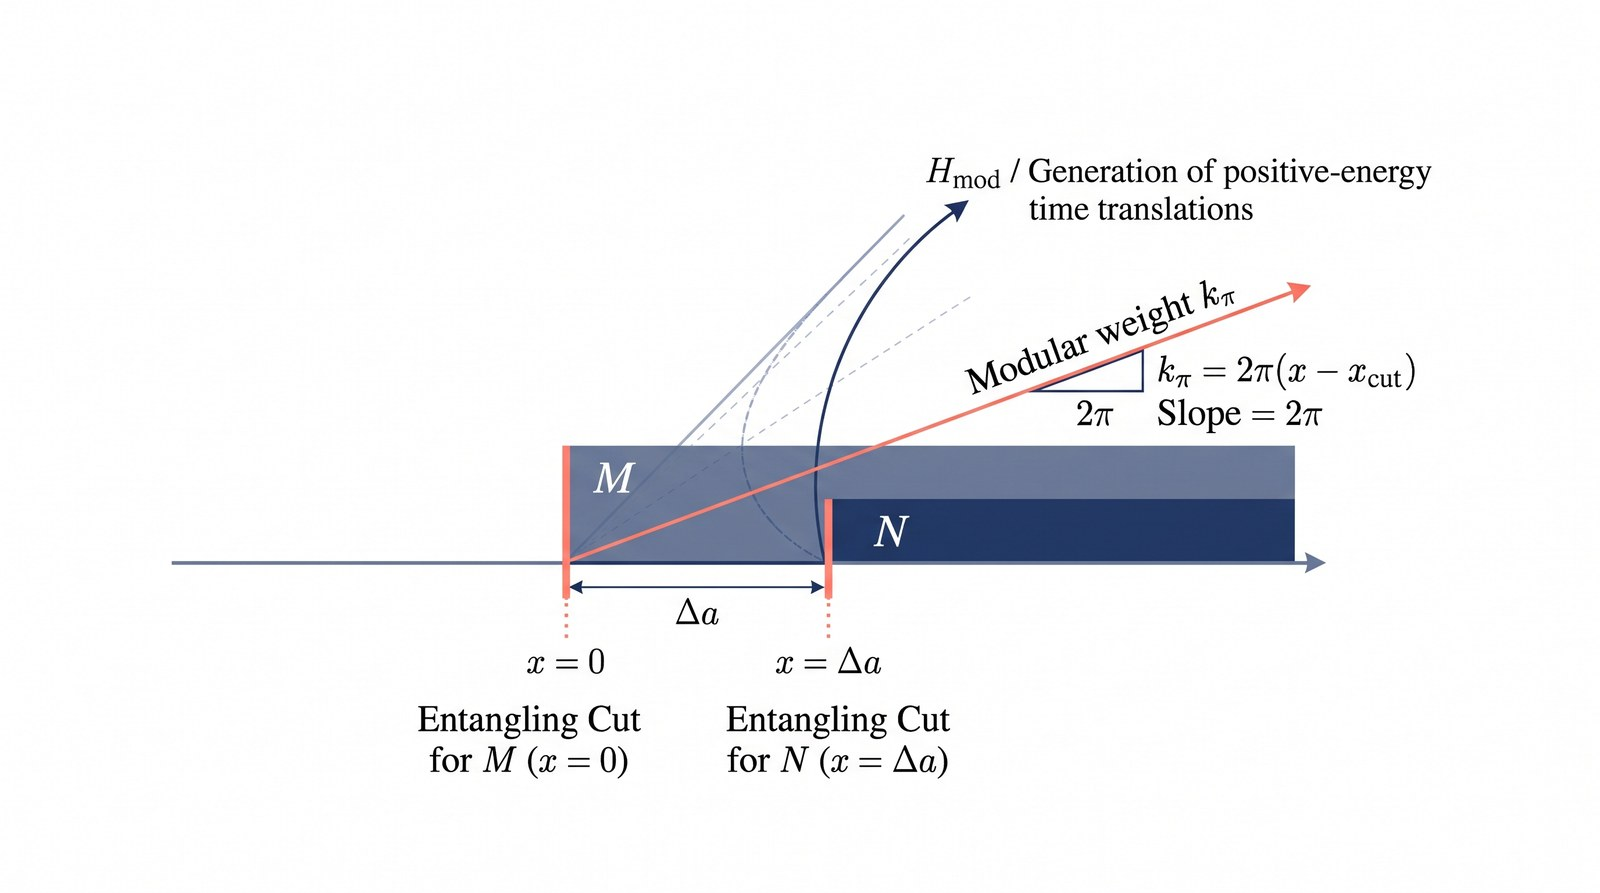
\includegraphics[width=0.80\textwidth]{figures/fig_modular_inclusion.jpg}
\caption{Proposition~\ref{prop:modular}. Two nested half-spaces, $M=\{x_1>0\}$ and $N=\{x_1>\Delta a\}$, with their entangling cuts. The modular Hamiltonian of a half-space weights the energy density with $2\pi(x_1-a)$, the straight line of slope $2\pi$; differentiating with respect to the position $a$ of the cut gives the energy \eqref{eq:HfromK}, and for a nested pair with the stated modular property there are translations with a positive generator (curved arrow). Schematic, produced as stated in the caption of Figure~\ref{fig:sketch}: the symbol $k_\pi$ and the words ``modular weight'' are not notation of this paper, and the dashed lines carry no meaning.}\label{fig:modular}
\end{figure}

Part (ii) says that a positive-energy translation group is determined by the state and two nested algebras alone. In the present setting the nesting is a spatial displacement of the entangling surface inside the reconstructed slice, and \eqref{eq:HfromK} expresses the energy of a region by the response of its modular Hamiltonian to this displacement. For Gaussian states everything is explicit: the modular Hamiltonian of a block with covariance $X\oplus P$ is $\tfrac12(\phi,k_\phi\phi)+\tfrac12(\pi,k_\pi\pi)$ with $k_\phi=X^{-1/2}O\,\nu\epsilon\,O^{T}X^{-1/2}$, $k_\pi=X^{1/2}O\,(\epsilon/\nu)\,O^{T}X^{1/2}$, where $X^{1/2}PX^{1/2}=O\nu^2O^{T}$ and $\epsilon=\ln\frac{\nu+1/2}{\nu-1/2}$. On the lattice, near the boundary of a block, it has the Bisognano--Wichmann form, with $k_\pi$ diagonal and growing linearly with the distance from the cut, and with a slope that tends to $2\pi$ in the continuum limit (Appendix~\ref{app:num}; for the half-infinite chain this is the corner-transfer-matrix result of \cite{PeschelChung}). The Hamiltonian that was used to define the ground state is thus recovered from the state.

Three remarks delimit this. First, the modular Hamiltonian is not an entropic quantity of pairs of nodes; it requires the reduced state of a region, that is, more than the matrix $C_{ij}$, in line with Proposition~\ref{prop:Todd}. Second, the Bisognano--Wichmann property is a property of the vacuum; on a curved background it holds approximately at scales small compared with $\Lcurv$ for states of Hadamard type, and exactly only for special horizons. Third, the erroneous use of this theorem in the earlier manuscript concerned distances; its proper role in the present programme is to supply time.

With $h$ from Section~\ref{sec:recon} and $K$ from \eqref{eq:YP}, the data $(h,K)$ of the initial-value formulation are available. They are not constrained by anything in the present framework: every background has its ground state, so the constraint equations of general relativity, evaluated on the reconstructed $(h,K)$, merely define an energy and a momentum density. A principle that equates them to those of matter is what is missing (Section~\ref{sec:open}).

\section{Interacting systems}\label{sec:int}

Outside the Gaussian class the mutual information is not a function of the two-point functions. The deviation can be written exactly.

\begin{proposition}[Gaussian part and non-Gaussianity]\label{prop:nonG}
Let $\rho$ be a state of two nodes $A,B$ with finite second moments, and let $\rho^G$ be the Gaussian state with the same first and second moments, assumed to have all symplectic eigenvalues larger than $\tfrac12$. Then, whenever the entropies are finite,
\begin{equation}\label{eq:nonG}
I_\rho(A:B)=I_{\rho^G}(A:B)+D(\rho_{AB}\|\rho^G_{AB})-D(\rho_A\|\rho^G_A)-D(\rho_B\|\rho^G_B),
\end{equation}
where $D$ is the relative entropy. In particular $|I_\rho-I_{\rho^G}|\le D(\rho_{AB}\|\rho^G_{AB})$.
\end{proposition}

\begin{proof}
$\ln\rho^G$ is a quadratic polynomial in the canonical operators, so $\Tr\rho\ln\rho^G=\Tr\rho^G\ln\rho^G$ and $S(\rho^G)-S(\rho)=D(\rho\|\rho^G)$. The marginals of $\rho^G$ are the Gaussian states associated with the marginals of $\rho$. Inserting this into $I=S_A+S_B-S_{AB}$ gives \eqref{eq:nonG}; the bound follows from the monotonicity of the relative entropy under partial traces.
\end{proof}

\begin{corollary}[First order in a coupling]\label{cor:firstorder}
Let $\rho_\lambda$ be a family of states such that $\rho_0$ is Gaussian and $D(\rho_{\lambda}\|\rho^G_{\lambda})=O(\lambda^2)$ on $AB$. Then $I_{\rho_\lambda}(A:B)=I_G(\sigma_\lambda)+O(\lambda^2)$, where $I_G$ is the Gaussian formula evaluated on the covariance matrix $\sigma_\lambda$ of $\rho_\lambda$.
\end{corollary}

The hypothesis is the generic behaviour of the relative entropy of two states that differ at order $\lambda$; it is the statement that to first order the entropy changes by the expectation of the modular Hamiltonian of $\rho_0$, which is quadratic. For a weakly interacting field the consequence is that, to first order in the coupling, all statements of Section~\ref{sec:gauss} hold with the two-point functions of the interacting theory. By the K\"all\'en--Lehmann representation these are $Z$ times the free correlators with the physical mass, plus contributions from the continuum that decay faster; hence the decay law \eqref{eq:decay} holds with the physical mass and an additional factor $Z^2$, and the profile assumption is stable at this order.

Beyond first order the non-Gaussian term in \eqref{eq:nonG} is of order $\lambda^2$. We expect it to decay at the same rate $e^{-2mr}$, since the connected correlations of composite operators such as $\phi^2$ are mediated by two-particle exchange, but we have no proof. A bound in one direction holds for all states: the mutual information is additive, lower semicontinuous, invariant under local unitaries and strongly superadditive, $I(A_1A_2:B_1B_2)\ge I(A_1:B_1)+I(A_2:B_2)$, which are the hypotheses under which Wolf, Giedke and Cirac \cite{WGC} prove that a functional is minimised, at fixed covariance matrix, by the Gaussian state. If their lemma applies as we read it, then $I_\rho\ge I_{\rho^G}$ for every state, which strengthens the bound $I\ge\tfrac12(\text{correlation})^2$ of \cite{WVHC}: correlations in an interacting theory can only decay more slowly than the Gaussian formula predicts. For continuous-variable nodes an upper bound of the same form is equivalent to a bound on the non-Gaussianity $D(\rho_{AB}\|\rho^G_{AB})$ of pairs of distant nodes, and is open.

\subsection{A two-sided bound for finite-dimensional nodes}

For nodes with finitely many levels the rate of decay can be controlled non-perturbatively.

\begin{theorem}[Mutual information and clustering]\label{thm:cluster2}
Let $A,B$ have dimensions $d_A,d_B$, let $\rho_A,\rho_B$ be faithful with smallest eigenvalues $\lambda_A,\lambda_B$, and let
\begin{equation}
\gamma=\sup\big\{|\langle E\otimes F\rangle-\langle E\rangle\langle F\rangle|:\ \|E\|,\|F\|\le1\big\}.
\end{equation}
Then
\begin{equation}\label{eq:twosidedMI}
\tfrac12\gamma^2\le I(A:B)\le\frac{(d_A^2-1)(d_B^2-1)}{\lambda_A\lambda_B}\,\gamma^2 .
\end{equation}
\end{theorem}

\begin{proof}
The lower bound is Pinsker's inequality, $I\ge\tfrac12\|\rho_{AB}-\rho_A\otimes\rho_B\|_1^2$, as in \cite{WVHC}. For the upper bound let $\varsigma=\rho_A\otimes\rho_B$. The relative entropy is dominated by the sandwiched R\'enyi divergence of order two, so $I=D(\rho_{AB}\|\varsigma)\le\ln\Tr(\varsigma^{-1/2}\rho_{AB}\varsigma^{-1/2}\rho_{AB})$. Choose bases $E_a$ of the operators on $A$ and $F_b$ on $B$ that are orthonormal for $\langle E,E'\rangle_A=\Tr(\rho_A^{1/2}E^*\rho_A^{1/2}E')$, respectively $\langle\cdot,\cdot\rangle_B$, with $E_0=F_0=\mathbf 1$. Expanding $\varsigma^{-1/2}\rho_{AB}\varsigma^{-1/2}$ in the product basis, its coefficients are $\langle E_a^*\otimes F_b^*\rangle_\rho$ and
\[
\Tr(\varsigma^{-1/2}\rho_{AB}\varsigma^{-1/2}\rho_{AB})=1+\sum_{a,b\ge1}\big|\langle E_a^*\otimes F_b^*\rangle_\rho\big|^2 ,
\]
the terms with exactly one index equal to zero being $\langle E_a^*\rangle=\langle E_a,\mathbf 1\rangle_A=0$. For $a,b\ge1$ the expectation values are connected correlations, bounded by $\gamma\|E_a\|\|F_b\|$, and $1=\langle E_a,E_a\rangle_A\ge\lambda_A\|E_a\|^2$. With $\ln(1+s)\le s$ this gives \eqref{eq:twosidedMI}.
\end{proof}

\begin{corollary}[Gapped lattice systems]\label{cor:gapped}
For the ground state of a gapped local Hamiltonian on a lattice of finite-dimensional sites, with faithful single-site states, $I(i:j)\le Ce^{-2r/\xi_c}$, where $\xi_c$ is the correlation length of the exponential clustering theorem \cite{HastingsKoma}. If the clustering is sharp and isotropic, $\gamma\ge c\,r^{-p}e^{-r/\xi_c}$, then with $\xi_0=\xi_c/2$ the surprisal distance satisfies $d_C=r+O(\xi_0\ln r)$.
\end{corollary}

So for lattice systems with finite-dimensional sites the mutual information decays at exactly twice the rate of the correlations, interacting or not, and the surprisal distance has the same structure as in Corollary~\ref{cor:drift}: the Riemannian distance plus a logarithmic drift. What is not obtained is the profile assumption in its exact form: the drift need not be a function of $r$ alone. This is not needed: condition (W1) of Hypothesis~\ref{hyp:window} does not ask $d_C-d_{ij}$ to be a function of the distance. If the sites are sampled as in Assumption~\ref{ass:profile} and the clustering is sharp and isotropic, so that (W1) and (W2) hold with $\Delta=O(\xi_0\ln(1/\xi_0))$, Theorem~\ref{thm:window} applies whenever $\xi_0\ln(1/\xi_0)\sqrt{\ln(1/\xi)}\ll\xi$; we have not verified (W2) for lattice systems in detail. For continuous-variable nodes the argument requires a replacement for $\lambda_A^{-1}$ and is open.

\section{Matter and the missing principle}\label{sec:matter}

\paragraph{Matter is invisible without backreaction} Suppose the system consists of the gapped field of Section~\ref{sec:gauss}, which carries the correlations $C_{ij}$, and of further fields (``matter''), and that the state is a product of a state of the gapped field on a given background and an arbitrary state of matter. Then the $C_{ij}$, and with them the reconstructed $h$ and $K$, do not depend on the state of matter. A coupling of geometry to matter is therefore not contained in the kinematics developed so far; it requires a principle that correlates the background with the matter content.

\paragraph{Self-consistency selects nothing} One might hope that the requirement ``the geometry reconstructed from the state is the geometry on which the state was defined'' singles out particular geometries. It does not: by the theorems of Sections~\ref{sec:recon}, \ref{sec:gauss} and \ref{sec:time} the reconstruction returns $(h,K)$ for the ground state on \emph{every} background, so every background is a fixed point of the map (background $\to$ state $\to$ reconstructed geometry). A selection can only come from an extremal principle or from a constraint that involves matter.

\paragraph{Two candidate principles} Both of the following are formulated without a gravitational action.

\emph{(P1) No external geometry.} The total effective action of all sectors is stationary with respect to the background metric, $\langle T_{\mu\nu}\rangle_{\mathrm{total}}=0$. For the gapped sector the effective action is the induced action of Remark~\ref{rem:induced}.

\emph{(P2) Entanglement equilibrium.} For every small geodesic ball the total entanglement entropy is stationary under variations of the state and the geometry at fixed volume \cite{Jacobson16}.

\begin{proposition}[The two principles agree]\label{prop:principles}
Let $D=3$, let the gapped sector consist of minimally coupled fields with induced constants $M_{\mathrm{ind}}^2$ and $\rho_{\mathrm{vac}}$, and let the matter sector be described by a quantum field theory with energy--momentum tensor $T^{\mathrm{mat}}_{\mu\nu}$ whose scales are large compared with the radius $\ell$ of the balls, which in turn is large compared with $1/m$. Then (P1), to leading order in the curvature expansion, and (P2), to first order in the variations, both give
\begin{equation}\label{eq:induced}
M_{\mathrm{ind}}^2\,G_{\mu\nu}+\rho_{\mathrm{vac}}\,g_{\mu\nu}=\langle T^{\mathrm{mat}}_{\mu\nu}\rangle ,\qquad G_N=\frac{1}{8\pi M_{\mathrm{ind}}^2}.
\end{equation}
\end{proposition}

\begin{proof}[Justification]
(P1) is the variation of the induced action plus the matter action. For (P2), the argument of \cite{Jacobson16} yields Einstein's equation with a Newton constant fixed by the coefficient $\eta$ of the area law of the short-distance entanglement, $G_N=1/4\eta$. For minimally coupled fields the entanglement entropy across a surface equals $A/4G_{\mathrm{ind}}$ with the \emph{induced} Newton constant, because the same fluctuations renormalise both \cite{Jacobson94,Solodukhin}; hence $\eta=2\pi M_{\mathrm{ind}}^2$ and the two equations coincide. The cosmological term is not fixed by (P2).
\end{proof}

We state this as a proposition because the ingredients are established results, but it is conditional: neither principle is derived here. What the present paper adds is that both sides of \eqref{eq:induced} are accessible from the state. The left-hand side is built from $h$ (Section~\ref{sec:recon}), $K$ (Section~\ref{sec:time}) and, in the static case, the lapse (Section~\ref{sec:scalar}); the coupling $M_{\mathrm{ind}}^2$ is the area-law coefficient of the entanglement of the gapped sector, an entropic quantity; the right-hand side is a property of the matter state. The equation is then a constraint relating correlations of the geometric sector to expectation values in the matter sector.

\paragraph{Scales} The argument needs the window
\begin{equation}
\varepsilon\lesssim a\ll\frac1m\lesssim\xi\ll\ell\ll L_{\mathrm{mat}},\ \Lcurv ,
\end{equation}
with $\varepsilon$ the cutoff that sets $M_{\mathrm{ind}}^2=1/96\pi^2\varepsilon$, and $L_{\mathrm{mat}}$ the shortest scale of the matter state. With two sectors, a heavy one that carries the geometry and a light one that sources it, there is no conflict between the regime of Assumption~\ref{ass:profile} and that of the entanglement-equilibrium argument.

\paragraph{What the equation predicts for the data} In the static weak-field limit, $\dd s^2=-(1+2\Phi)\dd t^2+(1-2\Psi)\dd x^2$, \eqref{eq:induced} gives $\Delta\Psi=4\pi G_N\rho$ and $\Phi=\Psi$. In the correlation data this is a conformal change $\hat g=(1-2\Psi)\delta$ of the reconstructed spatial metric, that is, a change of the surprisal distances near matter, together with a lapse $\Omega=1+\Phi$ that appears in the prefactor $\Theta$ of Theorem~\ref{thm:vargap}. The equality $\Phi=\Psi$ is a relation between two independently measurable features of the correlations, the exponent and the prefactor.

\paragraph{A reading of (P1)} In the static case (P1) says that the total ground-state energy is stationary with respect to the spatial metric and the lapse. This is the Born--Oppenheimer condition for a slow degree of freedom: if the parameters of the gapped sector that we have called the background are themselves dynamical variables of a larger system, they sit at a stationary point of the energy of the fast degrees of freedom. In this reading (P1) is not an additional law but the statement that the background is not external. It is a reformulation, not a derivation; the kinetic term of the slow variables is supplied by Theorem~\ref{thm:xray} only at the level of the induced action.

\subsection{What the missing input is}\label{sec:central}

We collect four statements that locate the missing input precisely. None of them derives a field equation from the correlations; together they show what would.

\emph{(a) The gapped sector satisfies its own equation identically.} On every background the energy--momentum of the gapped sector in its ground state is, to leading orders in the curvature, $\langle T^{\mathrm{gap}}_{\mu\nu}\rangle=-\rho_{\mathrm{vac}}\,g_{\mu\nu}-M_{\mathrm{ind}}^2\,G_{\mu\nu}$, the variation of the induced action of Remark~\ref{rem:induced}. Equation \eqref{eq:induced} is therefore the statement $\langle T^{\mathrm{gap}}_{\mu\nu}\rangle+\langle T^{\mathrm{mat}}_{\mu\nu}\rangle=0$ and nothing else. The geometric side of Einstein's equation is always available; what is not given is the reason for the total to vanish.

\emph{(b) The entropic form can be computed directly.} Let $B$ be a geodesic ball of radius $\ell$ in a slice with $K=0$. From $\Vol(B)=\nu_D\ell^D(1-\tfrac{R\ell^2}{6(D+2)})$ and $A(\partial B)=D\nu_D\ell^{D-1}(1-\tfrac{R\ell^2}{6D})$, with $R$ the scalar curvature of the slice, the area at fixed volume differs from its flat value by $\delta A/A=-R\ell^2/2D(D+2)$, and $R=2G_{00}$ by the Hamiltonian constraint. With the area law $S^{\mathrm{gap}}=\eta A$ of the gapped sector and, for conformal matter, the first law $\delta S^{\mathrm{mat}}=2\pi\int_B\frac{\ell^2-r^2}{2\ell}\,\delta\langle T_{00}\rangle$,
\begin{equation}\label{eq:equilibrium}
\delta S^{\mathrm{gap}}\big|_V+\delta S^{\mathrm{mat}}=\frac{\nu_D\ell^{D+1}}{D+2}\Big(-\eta\,G_{00}+2\pi\,\delta\langle T_{00}\rangle\Big).
\end{equation}
The total entanglement entropy of all small balls is stationary at fixed volume if and only if $G_{00}=(2\pi/\eta)\langle T_{00}\rangle$ in every frame, which is Einstein's equation with $G_N=1/4\eta$; this is the computation behind (P2) \cite{Jacobson16}. Without matter it characterises the vacuum Einstein metrics as the backgrounds on which the entanglement of the gapped sector is stationary, a second characterisation next to Corollary~\ref{cor:fixed}.

\emph{(c) A local coupling does not suffice, and a scalar response gives the wrong theory.} If matter acts on the gapped field through a local interaction, its effect is a local change of the operator $A$, to leading order a change of the gap, $\delta m^2(x)\propto\langle\mathcal O^{\mathrm{mat}}(x)\rangle$. The correlations then change only where matter is; there is no long-range field. If the gap is controlled by a light scalar that is sourced by matter, a long-range response appears, but by Proposition~\ref{prop:lapse} a variable gap is the static spacetime $-\Omega^2\dd t^2+\Omega^2g$, which for flat $g$ is conformally flat.

\begin{proposition}[A scalar response is Nordstr\"om gravity]\label{prop:nordstrom}
If matter influences the correlations only through the gap, $m(x)=\bar m\,\Omega(x)$ on a flat optical metric, the reconstructed spacetime is $\Omega^2(-\dd t^2+\dd x^2)$. With $\Omega=1+\Phi$ it has the potentials $(\Phi,\Psi)=(\Phi,-\Phi)$ in the notation $-(1+2\Phi)\dd t^2+(1-2\Psi)\dd x^2$, whereas Einstein's equation requires $\Psi=\Phi$. Null geodesics are those of flat space.
\end{proposition}

\begin{figure}[t]
\centering
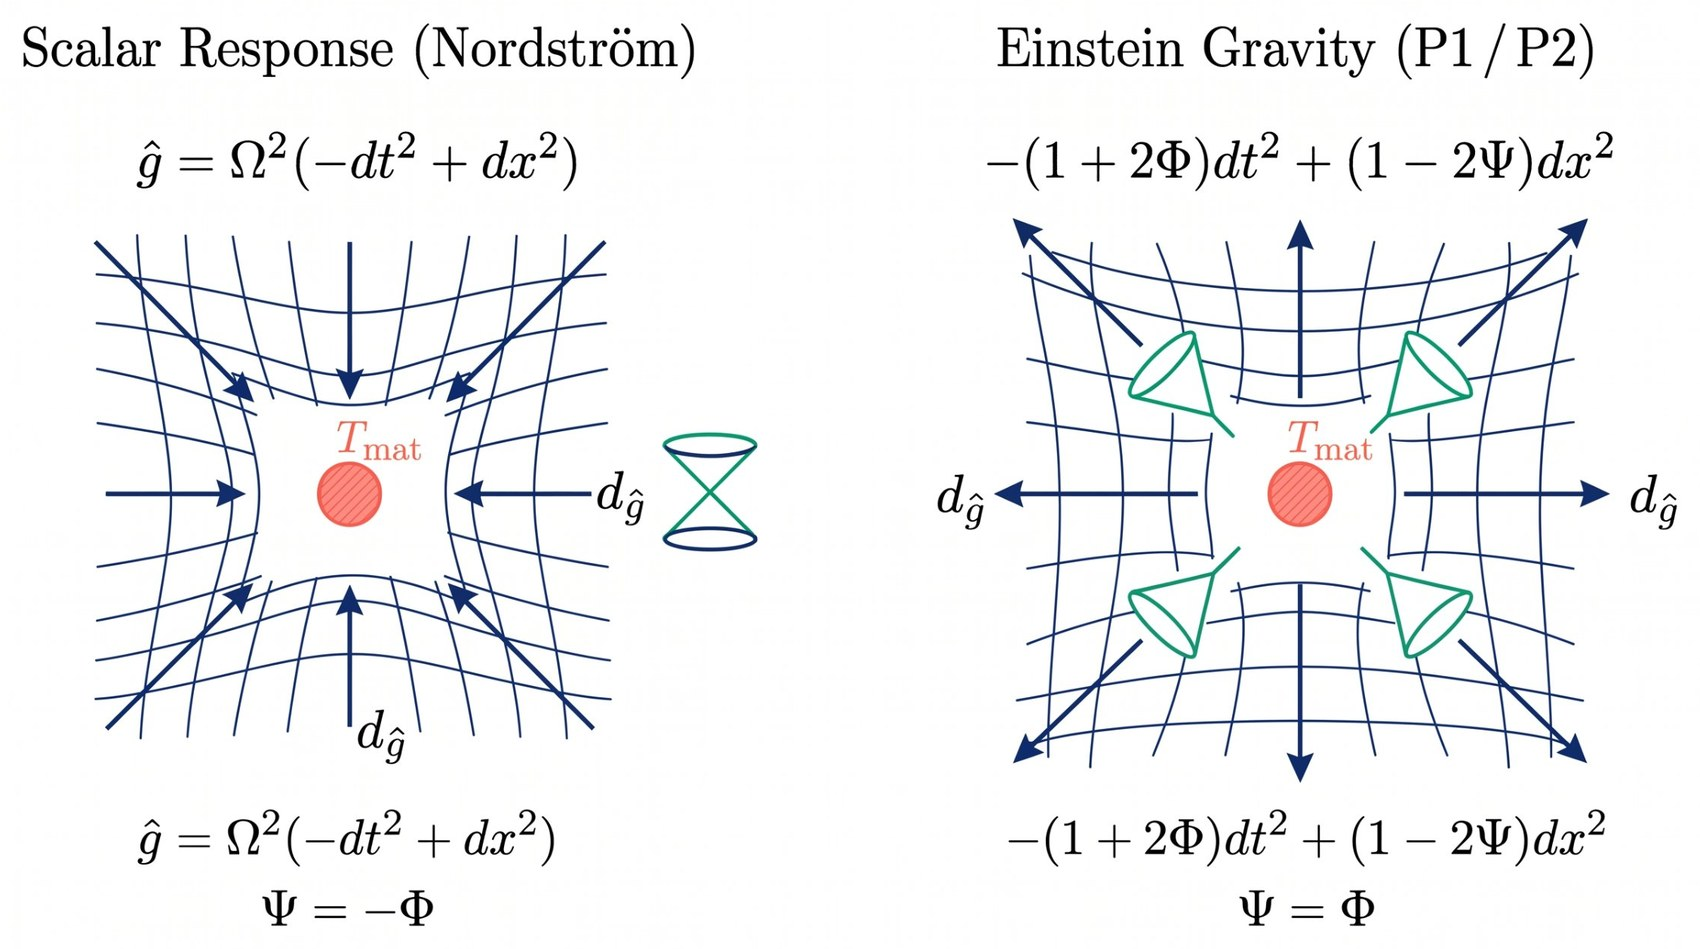
\includegraphics[width=0.84\textwidth]{figures/fig_nordstrom.jpg}
\caption{Proposition~\ref{prop:nordstrom}. Left: a scalar response gives the conformally flat metric $\Omega^2(-\dd t^2+\dd x^2)$ with $\Psi=-\Phi$; the reconstructed distances $d_{\hat g}$ near a mass become shorter and the light cones are those of flat space. Right: Einstein gravity, $\Psi=\Phi$; distances become longer and light is deflected. Schematic.}\label{fig:nordstrom}
\end{figure}


\begin{proof}
Proposition~\ref{prop:lapse} with $g=\delta$; conformally related metrics have the same null geodesics.
\end{proof}

In the data the two cases differ in sign: near a mass, where the lapse is reduced, the reconstructed distances $d_{\hat g}$ are shortened in the scalar case and lengthened in Einstein's theory. Einstein gravity requires that matter changes the optical metric, $g=n^2\delta$ with $n=1-2\Phi$, in addition to the gap $\Omega=1+\Phi$; the optical metric is the short-distance structure of the gapped sector, not a parameter of its state. A dynamical scalar (``dilaton'') is therefore not a route to Einstein's equation in this framework, in agreement with the fact that it is the conformal mode (Proposition~\ref{prop:conformal}).

\emph{(d) What would derive (P1).} Suppose that the background $q$ (the optical metric and the gap, or on a lattice the couplings that define the gapped Hamiltonian) is not an external parameter but is summed over, with no action of its own: $Z=\int\mathcal Dq\;Z^{\mathrm{gap}}[q]\,Z^{\mathrm{mat}}[q]$. For $\mathcal N$ fields in the gapped sector $-\ln Z^{\mathrm{gap}}[q]$ is $\mathcal N$ times the induced action, so that $M_{\mathrm{ind}}^2\propto\mathcal N$, and the integral is dominated for large $\mathcal N$ by the stationary point, which is (P1), with fluctuations of relative order $1/\mathcal N$. In this sense
\begin{equation}
\text{(P1)}\quad\Longleftarrow\quad\text{the background is summed over}\ \ +\ \ \text{many fields},
\end{equation}
which is Sakharov's proposal \cite{Sakharov,Visser} expressed in the present terms; the Born--Oppenheimer reading above is its Hamiltonian form. Two caveats: the Euclidean action is unbounded below in the conformal mode, so the stationary point is not a minimum, and the measure $\mathcal Dq$ is not specified.

\subsection{Node systems and the covariance of the cutoff}\label{sec:nodecov}

\begin{figure}[t]
\centering
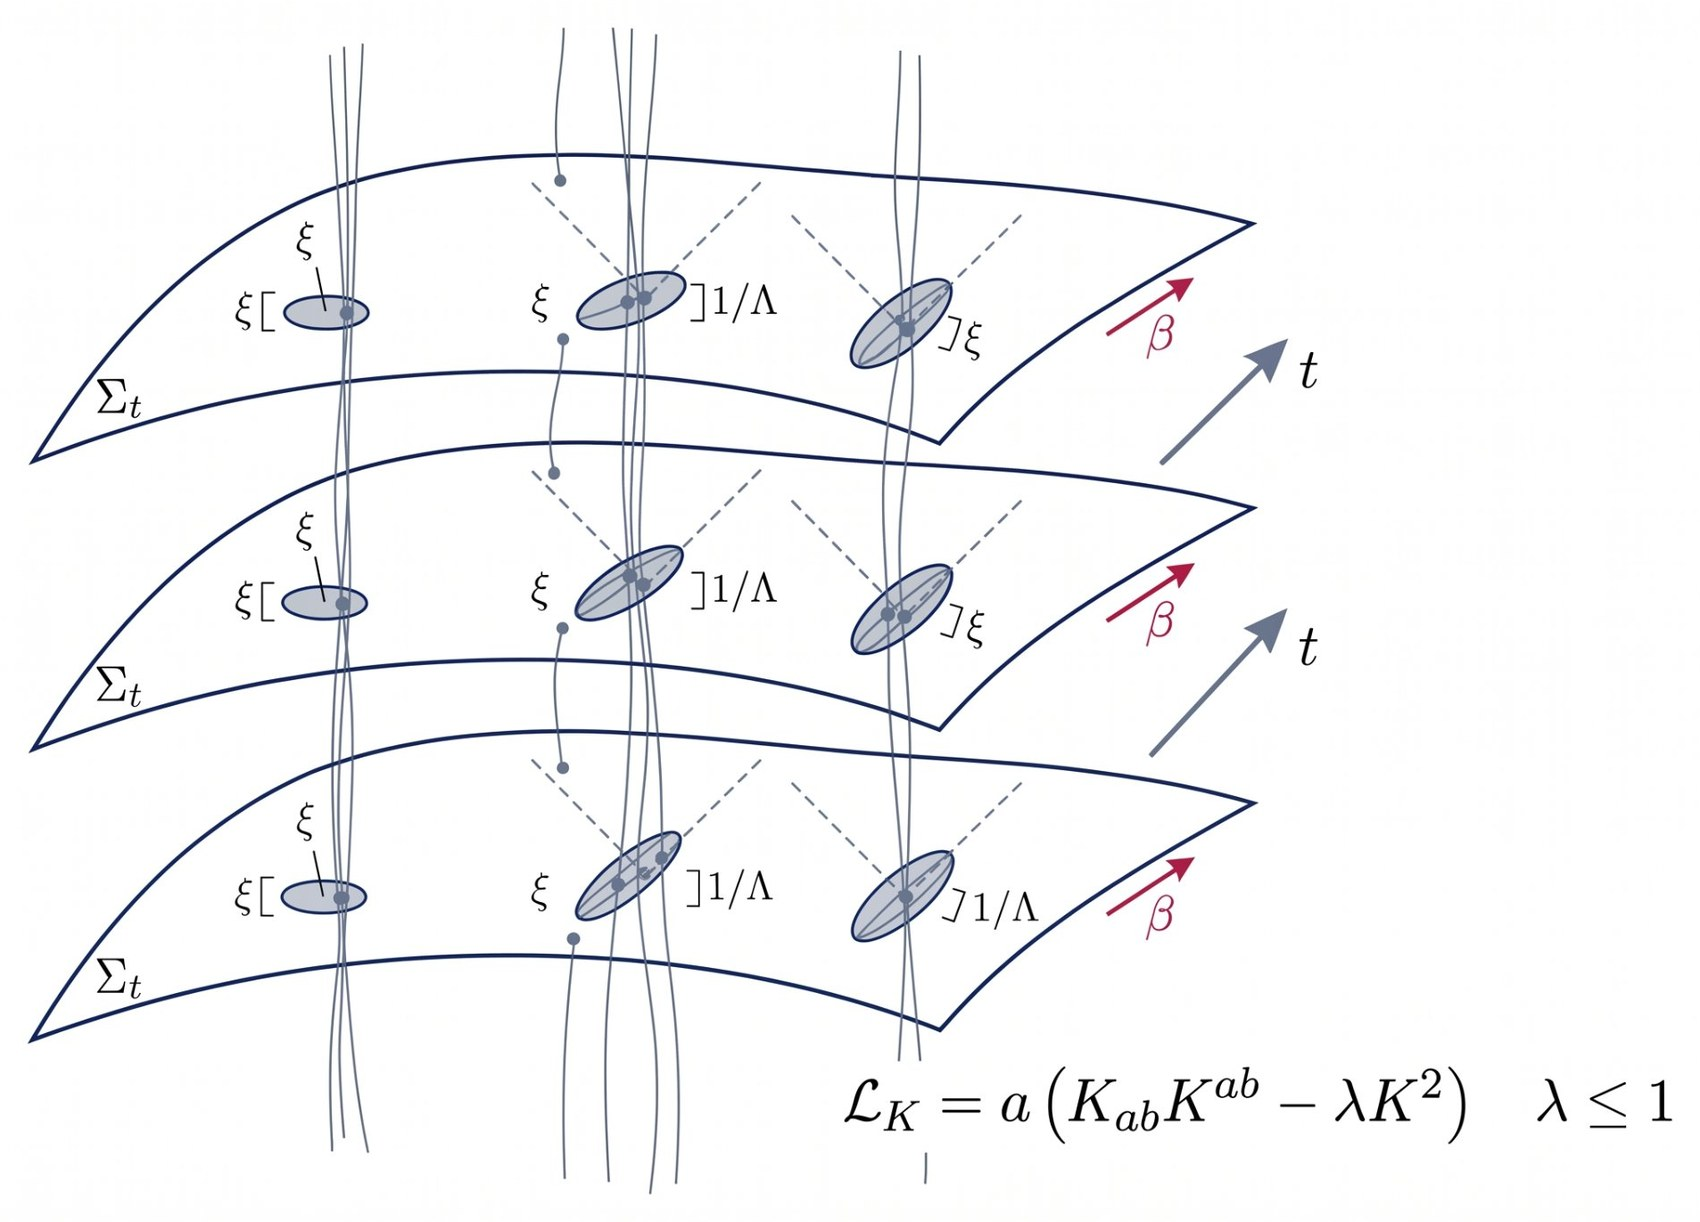
\includegraphics[width=0.74\textwidth]{figures/fig_foliation.jpg}
\caption{Node systems. Nodes that persist in time are worldlines; they define the slices $\Sigma_t$ and a cutoff that is at rest with respect to them (ellipses: the region resolved on a slice, of the size of the cutoff length; dashed: light cones). A shift $\beta$ moves the slices against the worldlines. The induced kinetic term is $L_K=a\,(K_{ab}K^{ab}-\lambda K^2)$ with $\lambda\le1$ (Proposition~\ref{prop:lambda}). Schematic; the labels on the ellipses all denote the cutoff length.}\label{fig:foliation}
\end{figure}

Statement (a) of Section~\ref{sec:central} and the induced action presuppose a covariant regularisation. For a system of nodes this fails at the order of the cutoff, and the failure cannot be repaired by the field content. We make this precise for the dependence of the ground-state energy on the shift, where the covariant answer is simple: on a closed flat slice with unit lapse a covariant action contributes, at second order in $\beta$,
\begin{equation}\label{eq:covshift}
-\tfrac12M_{\mathrm{ind}}^2\int\big(K_{ab}K^{ab}-K^2\big)=-\tfrac18M_{\mathrm{ind}}^2\int|\partial_a\beta_b-\partial_b\beta_a|^2 ,
\end{equation}
and nothing else, because the metric is flat up to a gauge transformation at first order in $\beta$, so that all other invariants are of fourth order. In particular a longitudinal shift $\beta=\nabla\chi$ must not change the energy.

\begin{proposition}[Shift response with a spatial cutoff]\label{prop:shiftresponse}
For the scalar field with Hamiltonian \eqref{eq:Hshift} on a flat slice, a cutoff $|k|\le\Lambda$ on the spatial momenta, and a shift whose gradient varies slowly on the scale $1/m$, the change of the ground-state energy at second order is $\int e_2\,\dd^Dx$ with
\begin{equation}\label{eq:e2}
e_2=-\frac1{16}\int_{|k|\le\Lambda}\frac{\dd^Dk}{(2\pi)^D}\,\frac{1}{\omega_k}\Big[\operatorname{tr}K-\frac{K(k,k)}{\omega_k^2}\Big]^2 .
\end{equation}
For $D=1$ this is $-K^2/24\pi$, independent of the mass and of $\Lambda\to\infty$. For $D\ge2$,
\begin{equation}\label{eq:e2div}
\begin{gathered}
e_2=-c_D\,\Lambda^{D-1}\,\big[(D^2-3)(\operatorname{tr}K)^2+2K_{ab}K^{ab}\big]+O(\Lambda^{D-3}),\\
c_D=\frac{\nu_D}{16\,(2\pi)^D(D-1)(D+2)} .
\end{gathered}
\end{equation}
\end{proposition}

\begin{proof}
In the notation of the proof of Theorem~\ref{thm:YP}, the component of $V|0\rangle$ with a pair of momenta $k,l$ has the amplitude $-\tfrac12\beta_b(k+l)\,[l_b\omega_k+k_b\omega_l]/\sqrt{\omega_k\omega_l}$. For $l=Q-k$ with $Q$ small, $l_b\omega_k+k_b\omega_l=Q_a(\delta_{ab}\omega_k^2-k_ak_b)/\omega_k+O(Q^2)$, so the amplitude is $-\tfrac12[\operatorname{tr}G-G_{ab}k_ak_b/\omega_k^2]$ with $G_{ab}=\partial_a\beta_b$ in Fourier space, and only the symmetric part $K$ of $G$ enters. Second-order perturbation theory divides the squared amplitude by $\omega_k+\omega_l\simeq2\omega_k$ and sums over unordered pairs, which gives \eqref{eq:e2}. For $D=1$ the bracket is $Km^2/\omega_k^2$ and $\int\dd k\,m^4/\omega_k^5=\tfrac43$. For $D\ge2$ the bracket tends to $\operatorname{tr}K-K(\hat k,\hat k)$, whose square has the angular average $[(D^2-3)(\operatorname{tr}K)^2+2K_{ab}K^{ab}]/D(D+2)$.
\end{proof}

The tensor structure in \eqref{eq:e2div} is not that of \eqref{eq:covshift}, the coefficient is of the same order $\Lambda^{D-1}$ as $M_{\mathrm{ind}}^2$, and a longitudinal shift lowers the energy. The lattice shows the same: in one dimension the lattice result for small lattice mass is $e_2=-K^2/12\pi$, the sum of the value $-K^2/24\pi$ of \eqref{eq:e2} and an equal contribution of the modes at the band edge, in agreement with the numerical value $-0.0264$; on a two-dimensional lattice a longitudinal shift $\beta_x(x)$ changes the energy by $-0.0165\int(\beta')^2$ and a trace-free shear $\beta_x(y)$ by $-0.0010\int(\beta')^2$, where \eqref{eq:covshift} demands zero for the first (Appendix~\ref{app:num}). Different non-covariant cutoffs thus give different finite or divergent non-covariant terms; a covariant one gives none.

\begin{proposition}[No cancellation by field content]\label{prop:nocancel}
Let the gapped sector consist of finitely many species, each in the ground state of a Hamiltonian $H_s(\beta)=H_{0,s}+\int\beta\cdot P_s$ on a Hilbert space that does not depend on $\beta$. Then for each species the second-order change $Q_s(\beta)$ of the ground-state energy is a non-positive quadratic form. Consequently $\sum_sQ_s(\nabla\chi)=0$ for all $\chi$, as required by covariance, holds if and only if $Q_s(\nabla\chi)=0$ for every species separately.
\end{proposition}

\begin{proof}
$E_{0,s}(\beta)=\inf_\psi\langle\psi,H_s(\beta)\psi\rangle$ is an infimum of functions that are affine in $\beta$, hence concave; explicitly $Q_s(\beta)=-\sum_n|\langle n|\int\beta\cdot P_s|0\rangle|^2/(E_n-E_0)\le0$. A sum of non-positive terms vanishes only if each term does.
\end{proof}

This is in contrast with the vacuum energy, where bosons and fermions enter with opposite signs (Proposition~\ref{prop:vacuum}). For the shift there is no such sign: every species of a node system lowers its energy under a longitudinal shift, and Proposition~\ref{prop:shiftresponse} shows that the scalar does so at leading order. The statement applies to every regularisation in which the degrees of freedom, and with them the cutoff, are fixed independently of the background; it does not apply to covariant schemes such as proper-time or Pauli--Villars regularisation, which do not correspond to a system of nodes with a positive Hilbert space. Nor does it apply when the Hamiltonian is not linear in the shift, as for a scalar field with a coupling to the curvature; see Sections~\ref{sec:fields} and~\ref{sec:content}, where cancellations between species do occur.

The origin of the obstruction is geometric. A system of nodes comes with two structures besides the metric: the world lines of the nodes, and the surfaces on which the Hamiltonian is defined, that is, a notion of simultaneity of the nodes. A cutoff tied to the nodes is a cutoff on these surfaces. In the setting of Proposition~\ref{prop:shiftresponse} the world lines are the orbits of a Killing field, so that their expansion and shear vanish and their acceleration is of second order in $\beta$; the response \eqref{eq:e2div} is a function of the extrinsic curvature of the surfaces. The induced action of a node system is therefore a functional of the metric \emph{and} of a foliation, with couplings of the order of $M_{\mathrm{ind}}^2$. This is the structure of Ho\v{r}ava gravity \cite{Horava} at low energies, which is equivalent to Einstein--aether theory \cite{JacobsonMattingly} with a hypersurface-orthogonal aether \cite{Jacobson10}.

That integrating out matter yields an action of this type is known when the matter itself violates Lorentz invariance: Nesterov and Solodukhin \cite{NS10} obtain a Ho\v{r}ava--Lifshitz effective action from fields with Lifshitz-type operators by heat-kernel methods, the matter-induced running of its couplings is computed with anisotropic heat kernels in \cite{DSS}, and in the spectral-action construction of \cite{LMP} the coupling $\lambda$ is fixed by the parameters of a generalised Dirac operator. The situation here differs in one respect: the fields are Lorentz invariant, with a relativistic dispersion, and only the regularisation, a fixed set of modes on the slices, singles out the foliation. The specific statements of this section, the response \eqref{eq:e2}, the inequality of Proposition~\ref{prop:lambda} and the values in Tables~\ref{tab:models} and~\ref{tab:species}, are to our knowledge not contained in these works. We have not compared coefficients with them; this would require a common regularisation.

Treating the background as a variable, as in Section~\ref{sec:central}(d), then yields such a theory and not general relativity. The spatial part of covariance is not affected: the reconstruction of Section~\ref{sec:recon} is independent of the sampling density, which is invariance under spatial diffeomorphisms of the node distribution. What is missing is invariance under local boosts. That a preferred frame at the cutoff scale is not suppressed at low energies is known for the matter sector \cite{Collins}; Propositions~\ref{prop:shiftresponse} and~\ref{prop:nocancel} are the corresponding statement for the induced gravitational action.

It is also known that a discrete structure can respect boost invariance only statistically, as a Poisson sprinkling of spacetime, and that no graph of finite valency can be associated with such a sprinkling in a Lorentz-invariant way \cite{BHS}. A kernel graph of subsystems on a slice is thus not a candidate for a Lorentz-invariant short-distance structure.

\subsection{The kinetic coupling of node systems}\label{sec:kinetic}

One may accept the preferred foliation and ask whether the resulting theory can agree with observation. The kinetic part of the low-energy action of Ho\v{r}ava gravity is
\begin{equation}\label{eq:horava}
L_K=a\,\big(K_{ab}K^{ab}-\lambda K^2\big),
\end{equation}
with $a=\tfrac12M_{\mathrm{ind}}^2$ and $\lambda=1$ in general relativity.

\begin{proposition}[Kinetic coupling of node systems]\label{prop:lambda}
Let the gapped sector be as in Proposition~\ref{prop:nocancel}, isotropic, and let the second-order change of its ground-state energy on a closed flat slice be local at leading order in derivatives of the shift. Then
\begin{equation}\label{eq:al}
E_2=-\frac a4\int|\partial_a\beta_b-\partial_b\beta_a|^2-\ell\int(\partial_a\beta_a)^2,\qquad a\ge0,\quad\ell\ge0,
\end{equation}
which is \eqref{eq:horava} with $\lambda=1-\ell/a$ when $a>0$. Hence $\lambda\le1$, with equality if and only if a longitudinal shift does not change the energy. For the scalar field with a momentum cutoff, $a=2c_D\Lambda^{D-1}$, $\ell=(D^2-1)c_D\Lambda^{D-1}$ and
\begin{equation}\label{eq:lambdaval}
\lambda=\frac{3-D^2}{2},\qquad\text{that is, }\lambda=-3\text{ for }D=3 .
\end{equation}
\end{proposition}

\begin{proof}
An isotropic quadratic form with two derivatives in $\beta$ is a combination of $\int\partial_a\beta_b\,\partial_a\beta_b$, $\int\partial_a\beta_b\,\partial_b\beta_a$ and $\int(\partial_a\beta_a)^2$; the last two agree after integration by parts, and the first equals $\tfrac12\int|\partial_a\beta_b-\partial_b\beta_a|^2+\int(\partial_a\beta_a)^2$. This gives the form \eqref{eq:al}; evaluating it on a transverse and on a longitudinal shift and using Proposition~\ref{prop:nocancel} gives $a\ge0$ and $\ell\ge0$. For a static configuration the Lagrangian is $-E_2$, and with $K_{ab}=\partial_{(a}\beta_{b)}$ one has $\int K_{ab}K^{ab}=\tfrac14\int|\partial_a\beta_b-\partial_b\beta_a|^2+\int(\partial_a\beta_a)^2$ and $\int K^2=\int(\partial_a\beta_a)^2$, so that $-E_2=\int[aK_{ab}K^{ab}-(a-\ell)K^2]$. The values for the scalar field follow by inserting the same two identities into \eqref{eq:e2div}.
\end{proof}

For comparison, \eqref{eq:covshift} is the case $a=\tfrac12M_{\mathrm{ind}}^2$, $\ell=0$. The value of $\lambda$ depends on the regularisation (the two-dimensional lattice numbers quoted above correspond to $\ell/a\approx8$), the inequality does not. We have attributed the transverse coefficient to the foliation; if part of it belongs to a twist term of the node world lines, $a$ in \eqref{eq:horava} is smaller, and $\lambda\le1$ still holds as long as the coefficient of $K_{ab}K^{ab}$ is positive, which is the condition that the tensor modes have positive kinetic energy.

The inequality has the wrong direction. For a homogeneous expansion $K_{ab}=Hh_{ab}$ in $D=3$, \eqref{eq:horava} gives $L_K=3a(1-3\lambda)H^2$, and the variation with respect to the lapse, which is the content of (P1), gives the Friedmann equation $\rho=3a(3\lambda-1)H^2$: the gravitational constant of cosmology is $2/(3\lambda-1)$ times that of the kinetic term. For $\lambda<\tfrac13$ a positive energy density admits no expanding solution; this includes \eqref{eq:lambdaval}. For $\tfrac13<\lambda<1$ the scalar mode of the theory is known to have a negative kinetic term \cite{GM}.

The observational bounds on the low-energy theory allow $0\le\lambda-1\lesssim0.1$, from primordial nucleosynthesis, together with much stronger bounds on the two other couplings from the speed of gravitational waves and from preferred-frame effects in the solar system \cite{GSS,OMW}. Stability and observation thus require $\lambda\ge1$, node systems give $\lambda\le1$, and the only common value is $\lambda=1$, the covariant case, which by Proposition~\ref{prop:lambda} requires the longitudinal response to vanish.

The statements on the scalar mode and on the bounds are taken from the literature on Ho\v{r}ava gravity and are not rederived here; they presuppose that the remaining terms of the induced action, the spatial curvature and the acceleration of the normals, complete \eqref{eq:horava} to the low-energy action of that theory. These terms are the subject of Section~\ref{sec:potential}.

\subsection{The potential sector}\label{sec:potential}

The low-energy action of the theory with a preferred foliation has two further terms,
\begin{equation}\label{eq:potential}
L=a\,\big(K_{ab}K^{ab}-\lambda K^2\big)+b_R\,R+b_a\,a_ia^i,\qquad a_i=\partial_i\ln N,
\end{equation}
with $R$ the scalar curvature of the slice and $N$ the lapse; in general relativity $b_R=a$ and $b_a=0$. The tensor modes propagate with $c_T^2=b_R/a$. We determine $b_a$, the coefficient $a$ for tensor modes, and $b_R$.

\begin{proposition}[Lapse]\label{prop:lapseresponse}
For the scalar field with Hamiltonian $\int N\,\mathcal H$, $\mathcal H=\tfrac12(\pi^2+|\nabla\phi|^2+m^2\phi^2)$, on a flat slice with a cutoff $|k|\le\Lambda$ and a lapse $N=1+\delta N$ that varies slowly on the scale $1/m$, the change of the ground-state energy at second order is
\begin{equation}\label{eq:lapse2}
E_2=-\frac1{64}\int\dd^Dx\int_{|k|\le\Lambda}\frac{\dd^Dk}{(2\pi)^D}\,\frac1{\omega_k^3}\Big[\Delta N-\frac{k_ak_b\,\partial_a\partial_bN}{\omega_k^2}\Big]^2 .
\end{equation}
It is of fourth order in derivatives; for $D=3$ it equals $-\frac{\ln(\Lambda/m)}{240\pi^2}\int(\Delta N)^2$ up to terms without the logarithm. In particular there is no term $\int|\nabla N|^2$ at the order $\Lambda^{D-1}$: $b_a=0$ at leading order.
\end{proposition}

\begin{proof}
With $\phi_k=(a_k+a_{-k}^*)/\sqrt{2\omega_k}$ and $\pi_k=-i\sqrt{\omega_k/2}\,(a_k-a_{-k}^*)$, the component of $\int\delta N\,\mathcal H\,|0\rangle$ with a pair of momenta $p,q$, $p+q=Q$, has the amplitude $\delta N_Q\,[m^2-p\cdot q-\omega_p\omega_q]/2\sqrt{\omega_p\omega_q}$. For $q=Q-p$ and small $Q$, $\omega_q=\omega_p-p\cdot Q/\omega_p+Q^2/2\omega_p-(p\cdot Q)^2/2\omega_p^3$, so that $m^2-p\cdot q-\omega_p\omega_q=-\tfrac12Q^2+(p\cdot Q)^2/2\omega_p^2+O(|Q|^3)$: the terms of order zero and one cancel. Second-order perturbation theory with the denominator $2\omega_p$ and the sum over unordered pairs gives \eqref{eq:lapse2}. For $D=3$ and large $k$ the square of the bracket has the angular average $\tfrac1{15}[6(\Delta N)^2+2|\partial\partial N|^2]$, $\int|\partial\partial N|^2=\int(\Delta N)^2$, and $\int\dd^3k/(2\pi)^3\,\omega_k^{-3}=\ln(\Lambda/m)/2\pi^2+O(1)$.
\end{proof}

This agrees with the covariant answer, in which $\int N\sqrt h\,R^{(4)}=\int N\sqrt h\,R$ for a static metric and no term $a_ia^i$ arises. As in Proposition~\ref{prop:nocancel}, $E_2\le0$ for every Hamiltonian that is linear in $N$, and $E_2=0$ for constant $N$. The pairs created by a gradient of the lapse cost four derivatives, those created by a gradient of the shift only two; this is why the lapse sector is harmless and the shift sector is not.

\begin{proposition}[Tensor kinetic term]\label{prop:tensorkin}
Let the field have the dispersion $\omega_k^2=W(k^2)$ on a fixed set of modes, and let the spatial metric in the coordinates of the nodes be $\delta_{ab}+\gamma_{ab}(t)$ with $\gamma$ trace-free, constant in space and slowly varying in time. The adiabatic effective Lagrangian at second order is $\tfrac14a\,\dot\gamma_{ab}\dot\gamma_{ab}$ per unit volume with
\begin{equation}\label{eq:aT}
a=\frac{1}{8D(D+2)}\int\frac{\dd^Dk}{(2\pi)^D}\,\frac{k^4\,W'(k^2)^2}{\omega_k^5}.
\end{equation}
For $W=k^2+m^2$ and $|k|\le\Lambda$ this is $a=2c_D\Lambda^{D-1}$, the transverse coefficient of Proposition~\ref{prop:lambda}.
\end{proposition}

\begin{proof}
The eigenvalue of $-\Delta_h$ on $e^{ik\cdot x}$ is $k^2-\gamma(k,k)$ to first order, so $\partial H/\partial\gamma_{ab}=-\tfrac12\sum_kW'(k^2)k_ak_b\,\phi_k\phi_{-k}$, which creates the pair $(k,-k)$ with amplitude $-W'\gamma(k,k)/2\omega_k$. The adiabatic kinetic energy of a parameter $\gamma(t)$ is $\sum_n|\langle n|\dot H|0\rangle|^2/(E_n-E_0)^3$; with $E_n-E_0=2\omega_k$ and the sum over unordered pairs this is $\sum_kW'^2\dot\gamma(k,k)^2/64\omega_k^5$, and the angular average of $\dot\gamma(\hat k,\hat k)^2$ is $2\dot\gamma_{ab}\dot\gamma_{ab}/D(D+2)$. In the relativistic case $\int\dd^Dk\,(2\pi)^{-D}k^4\omega_k^{-5}=D\nu_D\Lambda^{D-1}/(2\pi)^D(D-1)$ to leading order.
\end{proof}

So the kinetic coefficient of the tensor modes, computed for nodes that follow the normals of the slicing, is the same as the one obtained from a static shift, where the nodes follow a Killing field: in the transverse sector the node system respects the relation between the two that covariance demands.

The curvature term depends on how the cutoff is carried by a curved slice. If the ground-state energy is a function of the spectrum of the Laplacian of the slice, $E[h]=\Tr f(-\Delta_h)$ with $f$ of rapid decrease, the heat-kernel expansion gives
\begin{equation}\label{eq:specfun}
E[h]=(4\pi)^{-D/2}\Big[F_{D/2}\Vol+\frac{F_{D/2-1}}{6}\int R\,\dd V+\dots\Big],\qquad F_s=\frac1{\Gamma(s)}\int_0^\infty f(\lambda)\lambda^{s-1}\dd\lambda ,
\end{equation}
and $b_R=-(4\pi)^{-D/2}F_{D/2-1}/6$, since the Lagrangian of a static configuration is $-E$. The sign of $b_R$ is therefore opposite to that of $f$.

\begin{proposition}[Curvature term]\label{prop:curvterm}
\textup{(a)} If the modes below a fixed cutoff scale adapted to the metric contribute their zero-point energies, $f(\lambda)=\tfrac12\sqrt{\lambda+m^2}\,\eta(\lambda/\Lambda^2)$ with a profile $\eta\ge0$, then $b_R<0$: the energy increases with the total scalar curvature, and tensor modes have negative gradient energy.

\textup{(b)} If the number of modes is fixed and the dispersion saturates, $E=\tfrac12\sum_{k=1}^N\omega(\lambda_k)$ with $\omega$ increasing to $\omega_\infty$ and $f=-\tfrac12(\omega_\infty-\omega)$ of rapid decrease, then $E=\tfrac12N\omega_\infty+\Tr f(-\Delta_h)$ and $b_R>0$. For the field on the kernel graph with Gaussian profile, $\omega^2=\tfrac2{\xi^2}(1-e^{-\xi^2\lambda/2})$ in the continuum limit and for $m\xi\ll1$,
\begin{equation}\label{eq:graphE}
E=\frac{N\omega_\infty}2-\frac{1}{\sqrt2\,\xi}\sum_{j\ge1}c_j\Tr e^{\frac{j\xi^2}2\Delta_h},\qquad c_j=\Big|\binom{1/2}{j}\Big|,
\end{equation}
so that, with $\zeta_s=\sum_jc_jj^{-s}$,
\begin{equation}\label{eq:bRgraph}
\rho_{\mathrm{eff}}=-\frac{\zeta_{D/2}}{\sqrt2\,\xi\,(2\pi\xi^2)^{D/2}},\qquad b_R=\frac{\zeta_{D/2-1}\,\xi}{12\sqrt2\,(2\pi\xi^2)^{D/2}}>0 .
\end{equation}
\end{proposition}

\begin{proof}
(a) and the first part of (b) follow from \eqref{eq:specfun}, with $F_s>0$ in (a) and $F_s<0$ in (b). For \eqref{eq:graphE} use $1-\sqrt{1-x}=\sum_{j\ge1}c_jx^j$ with $x=e^{-\xi^2\lambda/2}$, and for \eqref{eq:bRgraph} insert $\Tr e^{s\Delta_h}=(4\pi s)^{-D/2}[\Vol+\tfrac s6\int R+O(s^2)]$ with $s=j\xi^2/2$; since $c_j\sim j^{-3/2}$ the sums converge for $D\ge2$, and the terms with $j\xi^2\gtrsim1$ are of lower order.
\end{proof}

The covariant proper-time regularisation corresponds to $f(\lambda)=\tfrac12\sqrt\lambda-1/2\sqrt{\pi\varepsilon}+\dots$, which is negative up to $\lambda\sim1/\varepsilon$: it is not a sum of positive zero-point energies, in accordance with the remark after Proposition~\ref{prop:nocancel}, and this is why it gives $b_R>0$. Among node systems, only those with a fixed number of modes share this sign; persistent nodes are thus required for the right sign of the curvature term, while they are the origin of the wrong sign of $\lambda-1$. In case (b) the volume term is of the covariant form $\rho_{\mathrm{eff}}\int\sqrt h$ with $\rho_{\mathrm{eff}}<0$. Two variants behave differently at the order of the vacuum energy. For a relativistic dispersion with the $N$ lowest modes, the two-term Weyl law gives, for $D=3$ and formally for a sharp cutoff, $b_R=+\Lambda^2/96\pi^2$, but the vacuum energy depends on the density $n$ of the nodes as $\int n^{(D+1)/D}h^{-1/2D}$: the nodes form a medium with pressure $\rho/D$, not a cosmological term. For a fixed set of modes in the coordinates of the nodes, such as a lattice with a fixed Brillouin zone, a constant trace-free $\gamma$ costs the energy $\frac{2D+3}{8D(D+2)}\operatorname{tr}\gamma^2\int\frac{\dd^Dk}{(2\pi)^D}|k|$, a mass term for the tensor modes at the scale of the cutoff.

\paragraph{Tensor speed and preferred-frame parameters} In the most favourable case, the field on the kernel graph, \eqref{eq:aT} and \eqref{eq:bRgraph} give for $D=3$
\begin{equation}\label{eq:cT}
a=4.52\cdot10^{-4}\,\xi^{-2},\qquad b_R=2.65\cdot10^{-3}\,\xi^{-2},\qquad c_T^2=\frac{b_R}{a}=5.87 ,
\end{equation}
in units in which the field itself propagates with speed one at long wavelengths. For the relativistic field with the $N$ lowest modes $c_T^2=5$, and in case (a) with a sharp cutoff $c_T^2=-5$. The two coefficients are different functionals of the dispersion, and no symmetry of a node system relates them; the observational bound is $|c_T-1|\lesssim10^{-15}$ \cite{OMW,GSS}. In the parametrisation of \cite{GSS}, \eqref{eq:potential} corresponds to $\beta=1-a/b_R$ and $\alpha=b_a/b_R$, and the preferred-frame parameter $\alpha_1$ is bounded by $|4(\alpha-2\beta)/(1-\beta)|\lesssim10^{-4}$. With $b_a=0$ this is the condition $8\,|c_T^2-1|\lesssim10^{-4}$, whereas \eqref{eq:cT} gives $39$. For the relativistic field with the $N$ lowest modes, where $\lambda=-3$ and $c_T^2=5$, the expressions of \cite{GSS} give $|\alpha_1|=32$ and $|\alpha_2|=12$, against bounds of $10^{-4}$ and $4\cdot10^{-7}$. These numbers are formal: the theory is already excluded by Proposition~\ref{prop:lambda}, and the post-Newtonian analysis presupposes a stable theory of the form \eqref{eq:potential}. They show that the acceleration term is the only part of the potential sector in which a node system agrees with general relativity. Other fields are treated in Section~\ref{sec:fields}, the longitudinal response of the field on the kernel graph in Section~\ref{sec:graphfields}. Not computed: corrections to \eqref{eq:graphE} from the sampling of the nodes.

\subsection{Other fields}\label{sec:fields}

The values above are for a minimally coupled scalar field. We add the Dirac field, the scalar field with a coupling to the curvature, and the Maxwell field.

\begin{proposition}[Dirac field]\label{prop:dirac}
Let $\psi$ be a Dirac field with $n_s$ spinor components on a flat slice, with one-particle Hamiltonian $\alpha\cdot p+\beta_{\mathrm D}m$, in the state in which the negative-energy modes with $|k|\le\Lambda$ are filled. Let the shift couple through $\tfrac12\{\beta_a,p_a\}-\tfrac i8\,\partial_a\beta_b\,[\alpha_a,\alpha_b]$; the second term is fixed by the requirement that a rigid rotation is generated by the total angular momentum.
\begin{enumerate}[label=\textup{(\roman*)}]
\item For a slowly varying shift with $K_{ab}=\partial_{(a}\beta_{b)}$ the second-order change of the energy density is
\begin{equation}\label{eq:e2dirac}
e_2=-\frac{n_s}{16}\int_{|k|\le\Lambda}\frac{\dd^Dk}{(2\pi)^D}\,\frac{1}{\omega_k^3}\Big[|Kk|^2-\frac{K(k,k)^2}{\omega_k^2}\Big]
=-n_sD\,c_D\Lambda^{D-1}\Big(K_{ab}K^{ab}-\frac{K^2}{D}\Big)+\dots
\end{equation}
Hence $a=n_sD\,c_D\Lambda^{D-1}$, $\ell=(1-\tfrac1D)a$ and $\lambda=1/D$.
\item The adiabatic kinetic term of a trace-free $\gamma_{ab}(t)$ is $\tfrac14a\,\dot\gamma_{ab}\dot\gamma_{ab}$ with the same $a$.
\item For $D=3$, $n_s=4$: with a cutoff of fixed scale adapted to the metric the energy increases with $\int R$, by twice the amount of a scalar field, so $b_R<0$; with a fixed number of modes and a sharp cutoff, formally, $b_R=+\Lambda^2/48\pi^2$.
\end{enumerate}
\end{proposition}

\begin{proof}
(i) For a homogeneous gradient the antisymmetric part of $\partial_a\beta_b$ generates a rotation, under which the state is invariant; only $K_{ab}\,\tfrac12\{x_b,p_a\}$ creates pairs. Let $u_s(k)$ and $w_{s'}(k)$ be the eigenspinors of $h(k)=\alpha\cdot k+\beta_{\mathrm D}m$ with energies $\omega_k$ and $-\omega_k$. First-order perturbation theory in $k$ gives $u_s^\dagger\,i\partial_{k_b}w_{s'}=-i\,u_s^\dagger\alpha_bw_{s'}/2\omega_k$, so the amplitude for a particle in $(k,s)$ and a hole in $(k,s')$ has modulus $|u_s^\dagger\,\alpha\!\cdot\!(Kk)\,w_{s'}|/2\omega_k$. With the projections $P_\pm=\tfrac12(1\pm h/\omega_k)$ and $h\,(\alpha\!\cdot\!q)=-(\alpha\!\cdot\!q)\,h+2k\!\cdot\!q$,
\[
\sum_{s,s'}|u_s^\dagger(\alpha\!\cdot\!q)w_{s'}|^2=\Tr\big[P_+(\alpha\!\cdot\!q)P_-(\alpha\!\cdot\!q)\big]=\frac{n_s}{2}\Big[q^2-\frac{(k\cdot q)^2}{\omega_k^2}\Big],
\]
and the energy denominator is $2\omega_k$; this is the first form of \eqref{eq:e2dirac}. For large $k$ the angular average of $|K\hat k|^2-K(\hat k,\hat k)^2$ is $(K_{ab}K^{ab}-K^2/D)/(D+2)$, and $\int\dd^Dk\,(2\pi)^{-D}|k|^{-1}=D\nu_D\Lambda^{D-1}/(2\pi)^D(D-1)$. The coefficients follow as in the proof of Proposition~\ref{prop:lambda}. (ii) Here $\dot H=-\tfrac12\dot\gamma_{ab}\alpha_ap_b$, which creates the same pairs with amplitude $\tfrac12u_s^\dagger\alpha\!\cdot\!(\dot\gamma k)w_{s'}$; the adiabatic formula of Proposition~\ref{prop:tensorkin} with $\dot\gamma=2K$ gives $-e_2$. (iii) $E=-\tfrac12\Tr|H_{\mathrm D}|$ and $H_{\mathrm D}^2=-\Delta+\tfrac14R+m^2$ on spinors, with first heat coefficient $(\tfrac16-\tfrac14)R$ per component; in \eqref{eq:specfun} both $f$ and this coefficient are negative. For a fixed number of modes the elimination of the cutoff by the two-term Weyl law reverses the sign of the curvature term, as for the scalar field.
\end{proof}

A massless Dirac field thus responds only to the trace-free part of $K_{ab}$: a shift $\beta=Hx$ generates a dilatation, under which it is invariant. The value $\lambda=1/D$ is the conformal point of \eqref{eq:horava}, at which the trace of $K_{ab}$ has no kinetic term and the Friedmann equation degenerates to $\rho=0$. For $N_s$ minimally coupled scalar fields and $N_d$ Dirac fields in $D=3$, with $a=2c_3\Lambda^2$, $\ell=8c_3\Lambda^2$ per scalar and $a=12c_3\Lambda^2$, $\ell=8c_3\Lambda^2$ per Dirac field,
\begin{equation}\label{eq:mixed}
\lambda=1-\frac{4(N_s+N_d)}{N_s+6N_d}\in\big[-3,\tfrac13\big],\qquad c_T^2=\frac{5(N_s+2N_d)}{N_s+6N_d}\in\big[\tfrac53,5\big],
\end{equation}
the second for a fixed number of modes. No content of minimally coupled scalar fields and Dirac fields reaches $\lambda>\tfrac13$ or $c_T=1$ (for other fields see below); for the content $N_s=4N_d$ that cancels the leading vacuum term (Proposition~\ref{prop:vacuum}), $\lambda=-1$ and $c_T^2=3$.

Proposition~\ref{prop:nocancel} assumes a Hamiltonian that is linear in the shift. A coupling $\tfrac12\zeta R^{(4)}\phi^2$ of a scalar field to the curvature violates this assumption, and it changes the picture.

\begin{proposition}[Non-minimally coupled scalar field]\label{prop:nonmin}
For the scalar field with the coupling $\tfrac12\zeta R^{(4)}\phi^2$, on a flat slice with lapse one and a cutoff $|k|\le\Lambda$,
\begin{equation}\label{eq:Hnonmin}
H=H_0+\int\pi\,\beta\!\cdot\!\nabla\phi+\zeta\int K\,\{\pi,\phi\}+\int\Big[2\zeta^2K^2+\frac\zeta2\big(K_{ab}K^{ab}-K^2\big)\Big]\phi^2,\qquad K=\partial_a\beta_a ,
\end{equation}
and to leading order in the cutoff
\begin{equation}\label{eq:alnonmin}
a=2c_D\big[1-2D(D+2)\zeta\big]\Lambda^{D-1},\qquad\ell=(D-1)\,c_D\big[(D+1)-8(D+2)\zeta\big]\Lambda^{D-1}.
\end{equation}
For $D=3$: $a=2c_3(1-30\zeta)\Lambda^2$, $\ell=8c_3(1-10\zeta)\Lambda^2$, $\lambda=(10\zeta-3)/(1-30\zeta)$. At the conformal value $\zeta=(D-1)/4D$ the energy depends only on the trace-free part of $K_{ab}$, $\lambda=1/D$, and $a=-(D^2+D-4)\,c_D\Lambda^{D-1}<0$. The adiabatic kinetic term of a trace-free $\gamma_{ab}(t)$ has the same coefficient $a$, and for a fixed number of modes and a sharp cutoff, formally, $b_R=(1-6\zeta)\Lambda^2/96\pi^2$ in $D=3$.
\end{proposition}

\begin{proof}
For lapse one, $R^{(4)}=R+K_{ab}K^{ab}-K^2+2\nabla_\mu(n^\mu K)$. After an integration by parts the last term gives $2\zeta K\phi\,\partial_n\phi$ in the Lagrangian, so $\pi=\partial_n\phi+2\zeta K\phi$, and the Legendre transformation gives \eqref{eq:Hnonmin}. The term $\int\pi\beta\cdot\nabla\phi$ creates the pair $(k,-k)$ with amplitude $-\tfrac i2[\operatorname{tr}K-K(k,k)/\omega_k^2]$, and $c\int\{\pi,\phi\}$ with amplitude $2ic$; hence the amplitude of the two terms that are linear in $\beta$ is $-\tfrac i2[(1-4\zeta)\operatorname{tr}K-K(k,k)/\omega_k^2]$, and
\begin{align*}
e_2={}&-\frac1{16}\int\frac{\dd^Dk}{(2\pi)^D}\frac1{\omega_k}\Big[(1-4\zeta)\operatorname{tr}K-\frac{K(k,k)}{\omega_k^2}\Big]^2\\
&+\Big[2\zeta^2K^2+\frac\zeta2\big(K_{ab}K^{ab}-K^2\big)\Big]\int\frac{\dd^Dk}{(2\pi)^D}\frac1{2\omega_k}.
\end{align*}
With the angular averages used before and $\int\dd^Dk\,(2\pi)^{-D}|k|^{-1}=16D(D+2)c_D\Lambda^{D-1}$, the coefficient of $K_{ab}K^{ab}$ is $-2c_D[1-2D(D+2)\zeta]\Lambda^{D-1}$, and evaluation on a longitudinal shift gives $\ell$. For trace-free $\gamma(t)$ the only new term is $\tfrac12\zeta K_{ab}K^{ab}\langle\phi^2\rangle$ with $K=\tfrac12\dot\gamma$, which changes $\tfrac14a$ by $-\tfrac1{16}\zeta\int\dd^Dk(2\pi)^{-D}\omega_k^{-1}$, the same shift. On a static slice the operator is $-\Delta+\zeta R+m^2$ with first heat coefficient $(\tfrac16-\zeta)R$.
\end{proof}

Three checks: at the conformal value the coefficient $2\zeta^2-\zeta(D-1)/2D$ of the term $K^2\langle\phi^2\rangle$ vanishes, as it must because $\beta=Hx$ then generates a dilatation; for $D=1$ the logarithmic divergences of the two terms of $e_2$ cancel, as covariance requires in two dimensions; and the cancellation \eqref{eq:N4} below. Since \eqref{eq:Hnonmin} is not linear in $\beta$, the energy is not concave: $a<0$ for $\zeta>1/2D(D+2)$ and $\ell<0$ for $\zeta>(D+1)/8(D+2)$. In particular the conformally coupled scalar field has $\lambda=1/D$, like the Dirac field, but a negative kinetic coefficient.

\begin{proposition}[Maxwell field]\label{prop:maxwell}
For the free Maxwell field in $D=3$ with the coupling $\int\beta\cdot(E\times B)$ and a cutoff $|k|\le\Lambda$ on the two transverse polarisations,
\begin{equation}\label{eq:e2maxwell}
e_2=-\int_{|k|\le\Lambda}\frac{\dd^3k}{(2\pi)^3}\,\frac{1}{4|k|}\Big[|K^\perp|^2-\tfrac12(\operatorname{tr}K^\perp)^2\Big]=-\frac{\Lambda^2}{40\pi^2}\Big(K_{ab}K^{ab}-\tfrac13K^2\Big),
\end{equation}
where $K^\perp$ is the projection of $K$ onto the plane orthogonal to $k$. Hence $a=24c_3\Lambda^2$, $\ell=16c_3\Lambda^2$, $\lambda=\tfrac13$. For a fixed number of modes and a sharp cutoff, formally, $b_R=-\Lambda^2/24\pi^2$.
\end{proposition}

\begin{proof}
With $F=E+iB$ the energy is $\tfrac12\int F^\dagger F$, the equation of motion is $i\partial_tF=(S\cdot p)F$ with the spin-one matrices $(S_a)_{bc}=-i\varepsilon_{abc}$, and $E\times B=\tfrac12F^\dagger SF$. The component of $F$ with wave vector $k$ is $\sqrt{2|k|}\,[e_+(k)a_{k,+}+e_-(k)a^*_{-k,-}]$, with $e_\pm(k)$ the eigenvectors of $S\cdot k$ with eigenvalues $\pm|k|$. The amplitude for the pair $(k,+)$, $(-k',-)$, $k-k'=Q$, is $\sqrt{|k||k'|}\,\beta_a(Q)\,e_+(k)^\dagger S_ae_-(k')$. It vanishes at $Q=0$ because $S_a$ changes the helicity by at most one, and to first order $e_-(k-Q)=e_-(k)+e_0\,\langle e_0,(S\cdot Q)e_-\rangle/|k|$ with the longitudinal vector $e_0=\hat k$. With $\langle e_+,S_ae_0\rangle=-\overline{(e_+)_a}$ and $\langle e_0,S_be_-\rangle=(e_-)_b$ the amplitude is $-K(e_-,e_-)$ for a symmetric gradient, of squared modulus $\tfrac12[|K^\perp|^2-\tfrac12(\operatorname{tr}K^\perp)^2]$; the energy denominator is $2|k|$. The angular average is $\tfrac25(K_{ab}K^{ab}-\tfrac13K^2)$. The transverse modes are the coexact one-forms of the slice; the first heat coefficient of the Hodge Laplacian on one-forms is $(\tfrac36-1)R$, that of the exact forms is $\tfrac16R$, so the transverse modes have $-\tfrac23R$, which is $-4$ times the scalar value.
\end{proof}

\begin{proposition}[Massive vector field]\label{prop:proca}
For the vector field of mass $m$ in $D=3$, with Hamiltonian $\tfrac12\int[E^2+(\nabla\!\cdot\!E)^2/m^2+B^2+m^2A^2]$ and a cutoff $|k|\le\Lambda$ on its three polarisations, the kinetic term for nodes that follow a homogeneous flow with gradient $K_{ab}$ is
\begin{equation}\label{eq:proca}
L_K=\frac{1}{16}\int_{|k|\le\Lambda}\frac{\dd^3k}{(2\pi)^3}\,\frac{1}{\omega_k}\Big[4K_{ab}K^{ab}-K^2+2x\,K\,K(\hat k,\hat k)+3x^2K(\hat k,\hat k)^2-8x\,|K\hat k|^2\Big],
\end{equation}
where $x=k^2/\omega_k^2$.
To leading order $a=26c_3\Lambda^2$, $\ell=24c_3\Lambda^2$, $\lambda=\tfrac1{13}$, the sums of the values of the Maxwell field and of a minimally coupled scalar field; for a fixed number of modes, formally, $b_R=-30c_3\Lambda^2$.
\end{proposition}

\begin{proof}
In a metric $h$ the Hamiltonian of the mode $k$ is $\tfrac12E^{T}\mathcal TE+\tfrac12A^{T}\mathcal VA$ with $\mathcal T_{ij}=(h_{ij}+k_ik_j/m^2)/\sqrt h$ and $\mathcal V^{jl}=\sqrt h\,[(h^{ab}k_ak_b+m^2)h^{jl}-k^jk^l]$; the pair $(A_i,E^i)$ is canonical for every $h$. For a Hamiltonian $\tfrac12p^{T}\mathcal Tp+\tfrac12q^{T}\mathcal Vq$ with frequencies $\omega_\alpha$ the adiabatic kinetic term is $\sum_{\alpha\beta}[\nu_{\alpha\beta}-\omega_\alpha\omega_\beta\tau_{\alpha\beta}]^2/8\omega_\alpha\omega_\beta(\omega_\alpha+\omega_\beta)^3$ with $\tau=\mathcal T^{-1/2}\dot{\mathcal T}\mathcal T^{-1/2}$ and $\nu=\mathcal T^{1/2}\dot{\mathcal V}\mathcal T^{1/2}$, which generalises \eqref{eq:adiab}. Here all three frequencies equal $\omega_k$, $\mathcal T^{1/2}=P_\perp+(\omega_k/m)P_\parallel$ with the projections along and across $k$, and with $\dot h_{ab}=2K_{ab}$ one finds $\|\nu-\omega_k^2\tau\|^2=4\omega_k^4$ times the bracket of \eqref{eq:proca}. The angular averages give $K_{ab}K^{ab}[4-\tfrac83x+\tfrac25x^2]+K^2[-1+\tfrac23x+\tfrac15x^2]$, and for $x\to1$ this is $\tfrac{26}{15}K_{ab}K^{ab}-\tfrac2{15}K^2$. On a static slice the transverse modes have the first heat coefficient $-\tfrac23R$ and the longitudinal ones $\tfrac16R$.
\end{proof}

For $m\to0$ the transverse part of \eqref{eq:proca} is the expression of Proposition~\ref{prop:maxwell}, and at large $k$ the longitudinal part is that of the minimally coupled scalar field. In the conditions of Corollary~\ref{cor:content} a massive vector field therefore counts as a Maxwell field and a scalar field with $\zeta=0$.

\begin{proposition}[Form fields in any dimension]\label{prop:pforms}
Let $A$ be a $p$-form gauge field on a slice of dimension $D\ge3$, $0\le p\le D-1$, with Hamiltonian $\tfrac12\int[|E|^2+|\dd A|^2]$ and a cutoff $|k|\le\Lambda$ on its transverse modes; $p=0$ is the minimally coupled scalar field and $p=1$ the Maxwell field. Let $n=D-1$, $d=\binom np$ the number of polarisations and $I=\binom{n-2}{p-1}$. In units of $c_D\Lambda^{D-1}$,
\begin{equation}\label{eq:pforms}
a=2d+4(D^2-4)\,I,\qquad\ell=(D^2-1)\,d,\qquad\kappa=d-6I,
\end{equation}
where $\kappa R/6$ is the first heat coefficient of the coexact $p$-forms.
\end{proposition}

\begin{proof}
The polarisations of the mode $k$ are the $p$-forms on the hyperplane orthogonal to $k$. In a metric $h$ the Hamiltonian of this mode is $\tfrac12E^{T}\mathcal TE+\tfrac12A^{T}\mathcal VA$ with $\mathcal T=h^{\otimes p}/\sqrt h$ and $\mathcal V=\sqrt h\,(h^{ab}k_ak_b)(h^{-1})^{\otimes p}$ on transverse forms. For $\dot h=2K$ this gives $\tau=2\rho(K^\perp)-\operatorname{tr}K$ and $\nu=k^2[\operatorname{tr}K-2K(\hat k,\hat k)-2\rho(K^\perp)]$, where $\rho$ is the representation of the Lie algebra of $n\times n$ matrices on $p$-forms, so the pair operator of Proposition~\ref{prop:proca} is $\nu-k^2\tau=2k^2[\operatorname{tr}K^\perp-2\rho(K^\perp)]$. With $\operatorname{tr}\rho(K)=\tfrac{pd}{n}\operatorname{tr}K$ and $\operatorname{tr}\rho(K)^2=I\,|K|^2+(\tfrac{pd}n-I)(\operatorname{tr}K)^2$,
\[
L_K=\int\frac{\dd^Dk}{(2\pi)^D}\,\frac{(d-4I)\,(\operatorname{tr}K^\perp)^2+4I\,|K^\perp|^2}{16\,|k|}.
\]
The angular averages are $\langle(\operatorname{tr}K^\perp)^2\rangle=[(D^2-3)K^2+2K_{ab}K^{ab}]/D(D+2)$ and $\langle|K^\perp|^2\rangle=[(D^2-2)K_{ab}K^{ab}+K^2]/D(D+2)$, and $\int\dd^Dk(2\pi)^{-D}|k|^{-1}=16D(D+2)c_D\Lambda^{D-1}$. This gives $a$ and the coefficient $(D^2-3)d-4(D^2-4)I$ of $K^2$, whose sum with $a$ is $\ell$. The Hodge Laplacian on $p$-forms has the first heat coefficient $[\tfrac16\binom Dp-\binom{D-2}{p-1}]R$; subtracting the exact forms, which are the coexact $(p-1)$-forms, recursively gives $\kappa$, and $\kappa=d-6I$ was verified for $D\le12$.
\end{proof}

The longitudinal coefficient does not depend on the spin, and $a$ and $\kappa$ are both linear in the index $I$ of the representation of the transverse rotations on the polarisations. Hence $a=b_R^{\mathrm{fix}}/D+\tfrac23(D^2-1)d$ for all form fields, where $b_R^{\mathrm{fix}}=-\tfrac23D(D^2-4)\,\kappa$ is the curvature coefficient at fixed cutoff scale; this is the structural origin of the relation between the kinetic and the curvature term for these fields. The formulas are invariant under the duality $p\leftrightarrow D-1-p$.

The coefficients $a$ of the scalar, Dirac and Maxwell fields are in the ratio $1:6:12$, the ratio of the normalisations of their stress-tensor two-point functions. Table~\ref{tab:species} collects the contributions of the three kinds of fields, in units of $c_3\Lambda^2=\Lambda^2/960\pi^2$.

\begin{table}[h]
\centering\small
\begin{tabular}{lcccc}
\toprule
field ($D=3$) & $a$ & $\ell$ & $b_R$ & zero-point energy\\
\midrule
scalar with coupling $\zeta$ & $2(1-30\zeta)$ & $8(1-10\zeta)$ & $10(1-6\zeta)$ & $+1$\\
Dirac & $12$ & $8$ & $20$ & $-4$\\
Maxwell & $24$ & $16$ & $-40$ & $+2$\\
massive vector & $26$ & $24$ & $-30$ & $+3$\\
\bottomrule
\end{tabular}
\caption{Contributions to \eqref{eq:potential} in units of $\Lambda^2/960\pi^2$, with $b_R$ for a fixed number of modes, and to the vacuum energy in units of that of one scalar field. General relativity requires $\sum\ell=0$ and $\sum b_R=\sum a>0$.}\label{tab:species}
\end{table}

\subsection{Field contents: cancellation at leading order, and the next order}\label{sec:content}

\begin{corollary}[Field contents]\label{cor:content}
For $N_s$ scalar fields with couplings $\zeta_1,\dots,\zeta_{N_s}$, $X=\sum_i\zeta_i$, $N_d$ Dirac fields and $N_v$ Maxwell fields, in units of $\Lambda^2/960\pi^2$,
\begin{equation}\label{eq:content}
\sum\ell=8\,(N_s+N_d+2N_v-10X),\qquad\sum b_R-\sum a=8\,(N_s+N_d-8N_v).
\end{equation}
Hence $\lambda=1$ and $c_T=1$ hold at leading order if and only if $N_s+N_d=8N_v$ and $X=N_v$, and then $\sum a=10\,(6N_v-N_s)$. If in addition the leading vacuum energy cancels, $N_s+2N_v=4N_d$, then $N_s=6N_v$, $N_d=2N_v$ and
\begin{equation}\label{eq:N4}
\sum a=\sum\ell=\sum b_R=0 .
\end{equation}
\end{corollary}

\begin{proof}
Sum the rows of Table~\ref{tab:species}; $X$ drops out of the second identity. The three conditions are linear in $N_s,N_d,N_v$ and have the stated solution.
\end{proof}

Two conclusions follow. First, the non-covariant terms of a node system \emph{can} cancel between species once the Hamiltonian is not linear in the shift: for example one scalar field with $\zeta=1$, seven Dirac fields and one Maxwell field give $\lambda=1$, $c_T=1$, $b_a=0$ and $\sum a=50>0$, the quadratic action of general relativity at the order $\Lambda^2$. The statement after Proposition~\ref{prop:nocancel} is therefore restricted to minimally coupled fields, and the conclusion of Sections~\ref{sec:kinetic} and~\ref{sec:potential} to field contents that do not satisfy the two conditions of Corollary~\ref{cor:content}; one of them is a condition on integers, the other requires the tuning of $X$.

Second, this does not yield a viable theory at leading order: such a content has a vacuum energy of the order $\Lambda^4$, which for a fixed number of modes is the energy of a medium at rest with respect to the nodes, and the content for which it cancels has no induced action at the order $\Lambda^2$ at all. That content, with $X=N_v$ realised by the conformal value $\zeta=\tfrac16$, is the field content of the maximally supersymmetric Yang--Mills multiplet; \eqref{eq:N4} is a consistency check of Table~\ref{tab:species}, though a weaker one than it appears (Remark~\ref{rem:reduced}). The next order is treated below.

For field contents with the cancellations of Corollary~\ref{cor:content} the induced action is determined by the terms of order $m^2\ln\Lambda$ and $m^2$. Let $L_m=\ln(2\Lambda/m)$.

\begin{proposition}[Mass terms]\label{prop:massterms}
For $D=3$ and a sharp cutoff, up to terms that vanish for $\Lambda\to\infty$, the coefficients of a scalar field with coupling $\zeta$, of a Dirac field and of a massive vector field are
\begin{equation}\label{eq:massterms}
\begin{gathered}
a=a_\Lambda-\frac{w\,m^2L_m}{96\pi^2}+\frac{a_{\mathrm f}\,m^2}{2880\pi^2},\qquad
b_R=b_\Lambda-\frac{w\,m^2L_m}{96\pi^2}+\frac{b_{\mathrm f}\,m^2}{2880\pi^2},\\
\ell=\ell_\Lambda+\frac{\ell_{\mathrm f}\,m^2}{2880\pi^2},
\end{gathered}
\end{equation}
where $a_\Lambda,b_\Lambda,\ell_\Lambda$ are the entries of Table~\ref{tab:species}, $b_R$ is for a fixed number of modes, and
\[
\begin{array}{lcccc}
 & w & a_{\mathrm f} & b_{\mathrm f} & \ell_{\mathrm f}\\
\text{scalar} & 1-6\zeta & 31-90\zeta & 15(1-6\zeta) & -6(1-20\zeta)\\
\text{Dirac} & 2 & 26 & 30 & -36\\
\text{massive vector} & -3 & -117 & -45 & -18
\end{array}
\]
In particular the logarithmic terms have the covariant form $-\frac{w\,m^2L_m}{96\pi^2}\,(K_{ab}K^{ab}-K^2+R)$, with the weights $w$ of the covariant computation, whereas the terms of order $m^2$ without logarithm do not: $b_{\mathrm f}-a_{\mathrm f}=-16$ for every scalar field, $+4$ for a Dirac field, $+72$ for a massive vector field, and $\ell_{\mathrm f}\neq0$.
\end{proposition}

\begin{proof}
With $A_n=\int_0^\Lambda k^{2n+2}\omega_k^{-2n-1}\dd k$ one has $A_0=\tfrac12\Lambda^2+\tfrac14m^2-\tfrac12m^2L_m$, $A_1=\tfrac12\Lambda^2+\tfrac54m^2-\tfrac32m^2L_m$ and $A_2=\tfrac12\Lambda^2+\tfrac{31}{12}m^2-\tfrac52m^2L_m$. Inserting them into the expression for $e_2$ in the proof of Proposition~\ref{prop:nonmin}, with the angular averages $\langle K(\hat k,\hat k)\rangle=\tfrac13K$ and $\langle K(\hat k,\hat k)^2\rangle=\tfrac1{15}(K^2+2K_{ab}K^{ab})$, gives for the scalar field the logarithmic part $\frac{m^2L_m}{96\pi^2}(1-6\zeta)(K_{ab}K^{ab}-K^2)$ and the stated finite parts; \eqref{eq:e2dirac} equals $-\frac{1}{8\pi^2}[\tfrac13K_{ab}K^{ab}A_1-\tfrac1{15}(K^2+2K_{ab}K^{ab})A_2]$ and gives the Dirac values. For $b_R$: the number of modes below $\Lambda$ is $\Lambda^3/6\pi^2+\kappa R\Lambda/24\pi^2$ per unit volume and the energy density is $\frac1{4\pi^2}\int_0^\Lambda k^2\omega_k\dd k+\kappa R\,(\Lambda^2+m^2L_m+\tfrac12m^2)/96\pi^2$, where $\kappa R/6$ is the first heat coefficient; eliminating $\Lambda$ at a fixed number of modes gives $\kappa R\,(-\Lambda^2+m^2L_m-\tfrac12m^2)/96\pi^2$. For the scalar field $\kappa=1-6\zeta$; for the filled Dirac sea the four components with $\kappa=-\tfrac12$ enter with a negative sign. For the vector field insert the $A_n$ into the angular average in the proof of Proposition~\ref{prop:proca}; $\kappa=-4+1$.
\end{proof}

The logarithms are thus universal and covariant, and the failure of covariance of a node system resides in the power terms and in the finite parts, which depend on the regularisation. The numbers $a_{\mathrm f},b_{\mathrm f},\ell_{\mathrm f}$ are those of the sharp cutoff.

\begin{proposition}[Independence of the cutoff profile]\label{prop:profile}
Let the modes enter with a weight $g(|k|/\Lambda)$, where $g$ is non-increasing, $g(0)=1$, and $\mu_p=\int_0^\infty s^p\,(-\dd g(s))$ is finite for $-2\le p\le4$; equivalently, average over sharp cutoffs $s\Lambda$ with the probability measure $-\dd g$. Then \eqref{eq:massterms} holds for $a$ and $\ell$ with $\Lambda^2$ replaced by $\mu_2\Lambda^2$, $L_m$ replaced by $L_m+\langle\ln s\rangle$, and the \emph{same} $a_{\mathrm f}$, $\ell_{\mathrm f}$. For a fixed total number of modes,
\begin{equation}\label{eq:bRprofile}
b_R=\frac{\kappa}{96\pi^2}\Big[\Lambda^2\Big(\frac{2\mu_1\mu_4}{\mu_3}-\mu_2\Big)-m^2\big(L_m+\langle\ln s\rangle\big)+m^2\Big(\frac{\mu_1\mu_2}{\mu_3}-\frac12\Big)\Big],
\end{equation}
with $\kappa=w$ as in Proposition~\ref{prop:massterms}. The ratios $q=2\mu_1\mu_4/\mu_2\mu_3-1$ and $r=\mu_1\mu_2/\mu_3$ satisfy $q\ge1$ and $r\le1$, with equality only for the sharp cutoff.
\end{proposition}

\begin{proof}
The coefficients are linear in the weight, and $g(|k|/\Lambda)=\int\theta(s\Lambda-|k|)\,(-\dd g(s))$. In \eqref{eq:massterms} for the cutoff $s\Lambda$ the finite parts do not depend on $s$; averaging replaces $s^2\Lambda^2$ by $\mu_2\Lambda^2$ and $\ln(2s\Lambda/m)$ by $L_m+\langle\ln s\rangle$, and the neglected terms are of order $m^4\mu_{-2}/\Lambda^2$. For $b_R$ the number of modes per unit volume is $\mu_3\Lambda^3/6\pi^2+\kappa R\mu_1\Lambda/24\pi^2$, the energy density is $(\mu_4\Lambda^4+\mu_2m^2\Lambda^2)/16\pi^2+\kappa R\,[\mu_2\Lambda^2+m^2(L_m+\langle\ln s\rangle)+\tfrac12m^2]/96\pi^2$ up to terms independent of $\Lambda$ and $R$, and the elimination of $\Lambda$ gives \eqref{eq:bRprofile}. The inequalities are the logarithmic convexity of the moments of a probability measure: $\mu_1\mu_4\ge\mu_2\mu_3$ and $\mu_1\mu_2\le\mu_3$.
\end{proof}

Thus the ratios of the leading coefficients $a$ and $\ell$, and with them the values of $\lambda$ in Table~\ref{tab:models}, the finite parts $a_{\mathrm f}$ and $\ell_{\mathrm f}$, and the first identity of \eqref{eq:content} do not depend on the profile. Only the curvature term does: the second identity of \eqref{eq:content} becomes $\sum b_R-\sum a=10q\,(N_s-6X+2N_d-4N_v)-2\,(N_s-30X+6N_d+12N_v)$ in units of $\mu_2\Lambda^2/960\pi^2$. With $\sum\ell=0$ the condition $c_T=1$ reads $q\,(2N_s+7N_d-26N_v)=-2N_s+3N_d+6N_v$, and together with $N_s+2N_v=4N_d$ it gives $(15q+5)(N_d-2N_v)=0$. Hence the last statement of Corollary~\ref{cor:content}, that the three conditions force \eqref{eq:N4}, holds for every profile.

\begin{corollary}[The next order]\label{cor:nextorder}
Let the terms of order $\Lambda^4$ and $\Lambda^2$ cancel, and put $M_s=\sum m_s^2$, $M_d=\sum m_d^2$, $M_v=\sum m_v^2$ for the scalar, Dirac and vector fields, and $Z=\sum\zeta_sm_s^2$. For every profile as in Proposition~\ref{prop:profile},
\begin{equation}\label{eq:nextorder}
\sum\ell=\frac{120Z-6M_s-36M_d-18M_v}{2880\pi^2},\qquad\sum a=\frac{(6Z-M_s-2M_d+3M_v)\,L}{96\pi^2}+O(m^2),
\end{equation}
with $L$ the logarithm at a common scale.
\begin{enumerate}[label=\textup{(\roman*)}]
\item Without massive vector fields, $\sum a>0$ for large $L$ implies $\sum\ell>0$ and
\begin{equation}\label{eq:lambdanext}
1-\lambda=\frac{20\,(6Z-M_s-2M_d)+14M_s+4M_d}{30\,(6Z-M_s-2M_d)\,L}>\frac{2}{3L}.
\end{equation}
\item In general, $\sum a>0$ for large $L$ and $\sum\ell\le0$ are compatible if and only if $7M_s+2M_d<39M_v$.
\item For the sharp cutoff $\sum(b_R-a)=(-16M_s+4M_d+72M_v)/2880\pi^2$; for a general profile the three numbers are $(30r-46)M_s-180(r-1)Z$, $60r-56$ and $162-90r$.
\end{enumerate}
\end{corollary}

\begin{proof}
Sum \eqref{eq:massterms} over the species, with Proposition~\ref{prop:profile}. $\sum a>0$ is $6Z>M_s+2M_d-3M_v$ and $\sum\ell\le0$ is $120Z\le6M_s+36M_d+18M_v$; an admissible $Z$ exists if and only if $20(M_s+2M_d-3M_v)<6M_s+36M_d+18M_v$, which is the inequality of (ii). For $M_v=0$ it fails, $\sum\ell>14M_s+4M_d>0$, and $1-\lambda=\sum\ell/\sum a$. (iii) uses $b_{\mathrm f}=30\kappa(r-\tfrac12)$ from \eqref{eq:bRprofile}.
\end{proof}

Without massive vector fields the result is negative: after all leading terms have been cancelled, a positive induced kinetic term comes with $\lambda<1$, the side on which the scalar mode has negative kinetic energy \cite{GM}, with a deviation of relative order $1/\ln(\Lambda/m)$; this uses neither the curvature term nor the condition $c_T=1$ and does not depend on the profile. With massive vector fields, which enter the covariant logarithm with the weight $-3$, the requirements $\sum a>0$, $\lambda=1$ and $c_T=1$ can be met together with the conditions of Corollary~\ref{cor:content} and the cancellation of the leading vacuum energy. An example for the sharp cutoff: one massive vector field of mass $m_v$, two massless Dirac fields, and five scalar fields, one with $m^2=\tfrac92m_v^2$ and $\zeta=\tfrac1{12}$ and four massless ones with $\sum\zeta=\tfrac{11}{12}$; then $\sum\ell=0$, $\sum(b_R-a)=0$ and $\sum a=\tfrac34m_v^2L/96\pi^2>0$. But this content has $\operatorname{Str}m^2\neq0$, and the next statements show that this cannot be avoided.

\begin{proposition}[Linear relations]\label{prop:relations}
Let $\operatorname{Str}f=\sum_{\mathrm{bosons}}f-\sum_{\mathrm{fermions}}f$, summed over the degrees of freedom, so that the vacuum energy density is $\frac1{16\pi^2}\operatorname{Str}\big[\Lambda^4+m^2\Lambda^2-\tfrac12m^4L_m+\tfrac18m^4\big]$. For every content of scalar fields with arbitrary couplings $\zeta$, Dirac fields, Maxwell fields and massive vector fields, with a sharp cutoff:
\begin{enumerate}[label=\textup{(\roman*)}]
\item at the order $\Lambda^2$, in units of $\Lambda^2/960\pi^2$,
\[
\sum a=\tfrac34\sum\ell-\tfrac14\sum(b_R-a)-2\operatorname{Str}1;
\]
\item at the order $m^2\ln\Lambda$, with $a=-w\,m^2L_m/96\pi^2$ and the finite parts in units of $m^2/2880\pi^2$,
\[
20\sum(-w\,m^2)=\sum\ell_{\mathrm f}m^2+\sum(b_{\mathrm f}-a_{\mathrm f})\,m^2+2\operatorname{Str}m^2;
\]
\item at the order $m^2$,
\[
\sum a_{\mathrm f}m^2=-\tfrac34\sum\ell_{\mathrm f}m^2-\tfrac74\sum(b_{\mathrm f}-a_{\mathrm f})\,m^2-\tfrac32\operatorname{Str}m^2 .
\]
\end{enumerate}
\end{proposition}

\begin{proof}
Each relation is linear in the content, so it suffices to verify it on the rows of Table~\ref{tab:species} and of the table in Proposition~\ref{prop:massterms}, where the row of the scalar field is split into its part independent of $\zeta$ and its part proportional to $\zeta$. For (i): $2=\tfrac34\cdot8-\tfrac14\cdot8-2$, $-60=\tfrac34\cdot(-80)$, $12=\tfrac34\cdot8-\tfrac14\cdot8+8$, $24=\tfrac34\cdot16+\tfrac14\cdot64-4$. For (ii): $-20=-6-16+2$, $120=120$, $-40=-36+4-8$, $60=-18+72+6$. For (iii): $31=\tfrac92+28-\tfrac32$, $-90=-\tfrac34\cdot120$, $26=27-7+6$, $-117=\tfrac{27}2-126-\tfrac92$.
\end{proof}

\begin{corollary}[Covariance and vanishing vacuum energy imply a vanishing induced action]\label{cor:vanish}
For the fields of Proposition~\ref{prop:relations}, if the non-covariant terms cancel, $\sum\ell=0$ and $\sum b_R=\sum a$, at the orders $\Lambda^2$ and $m^2$, and if $\operatorname{Str}1=\operatorname{Str}m^2=0$, then $\sum a=0$ at the orders $\Lambda^2$, $m^2\ln\Lambda$ and $m^2$: the induced action vanishes up to terms of order $m^4/\Lambda^2$. The conditions at the order $m^2$ determine the sums up to a common factor, $M_s:Z:M_d:M_v=5:1:2:1$, and this holds for every profile as in Proposition~\ref{prop:profile}.
\end{corollary}

\begin{proof}
The first statement is Proposition~\ref{prop:relations}. With $\operatorname{Str}m^2=M_s+3M_v-4M_d=0$ and $\sum\ell_{\mathrm f}m^2=0$ one finds $Z=\tfrac12M_d$, and the condition $\sum(b_{\mathrm f}-a_{\mathrm f})m^2=0$ of Corollary~\ref{cor:nextorder}(iii) becomes $(90r-150)(M_d-2M_v)=0$; since $r\le1$, $M_d=2M_v$, hence $M_s=5M_v$ and $Z=M_v$. On these values $6Z-M_s-2M_d+3M_v=0$, $\sum a_{\mathrm f}m^2=155-90+52-117=0$ and $\sum b_{\mathrm f}m^2=0$ for every $r$.
\end{proof}

The vanishing of $\operatorname{Str}m^2$ is not an optional requirement for a system with a fixed number of nodes. There the cutoff is tied to the density $n$ of the nodes, $\Lambda\propto(n/\sqrt h)^{1/3}$, and the terms $\Lambda^4$ and $m^2\Lambda^2$ of the vacuum energy are proportional to $h^{-1/6}$ and $h^{1/6}$ instead of $\sqrt h$: they are the energy of a medium at rest with respect to the nodes, not a cosmological term, and cannot be removed by a counterterm. The solution of Corollary~\ref{cor:vanish} has a simple realisation: five scalar fields, two Dirac fields and one massive vector field, all of the same mass, with $\sum\zeta=1$. These are the fields of a massive vector multiplet of maximally supersymmetric Yang--Mills theory, for which also $\operatorname{Str}m^4=0$.

\begin{remark}[Reduced form and status of the relations]\label{rem:reduced}
We have not found a derivation of Proposition~\ref{prop:relations} that covers all fields. What can be said is the following. All coefficients are linear functions of three numbers per field: $\kappa$, six times the first heat coefficient with the sign of the zero-point energy ($1-6\zeta$, $2$, $-4$, $-3$ for the scalar, Dirac, Maxwell and massive vector field); the signed number $d$ of degrees of freedom ($1$, $-4$, $2$, $3$); and a number $\nu$ that measures the deviation from conformal invariance ($1-6\zeta$, $0$, $0$, $1$). In the units of Table~\ref{tab:species} and of Proposition~\ref{prop:massterms},
\begin{equation}\label{eq:reduced}
\begin{aligned}
a&=-10\kappa-8d+20\nu,&\qquad\ell&=-\tfrac{20}{3}\kappa-\tfrac{16}{3}d+20\nu,&\qquad b_R&=10\kappa,\\
a_{\mathrm f}&=45\kappa+16d-30\nu,&\qquad\ell_{\mathrm f}&=10\kappa+14d-30\nu,&\qquad b_{\mathrm f}&=15\kappa,
\end{aligned}
\end{equation}
and Proposition~\ref{prop:relations} follows by eliminating $\kappa$ and $\nu$. In this form Corollary~\ref{cor:vanish} is immediate: $\ell=0$, $b_R=a$ and $d=0$ give $\nu=\kappa/3$ and $\nu=\kappa$, hence $\kappa=\nu=0$ and $a=0$, at both orders.

\emph{The leading order in any dimension.} Determining the coefficients from the scalar field with coupling $\zeta$ and the Dirac field in dimension $D$, with $\nu=1-\zeta/\zeta_{\mathrm c}$, $\zeta_{\mathrm c}=(D-1)/4D$, one finds in units of $c_D\Lambda^{D-1}$
\begin{equation}\label{eq:reducedD}
\begin{aligned}
a&=-\tfrac23D(D^2-4)\,\kappa-\tfrac13D(D^2-1)\,d+(D-1)^2(D+2)\,\nu,\\
\ell&=-\tfrac23(D-1)(D^2-4)\,\kappa-\tfrac13(D-1)(D^2-1)\,d+(D-1)^2(D+2)\,\nu .
\end{aligned}
\end{equation}
The first term of $a$ is exactly the curvature coefficient at fixed cutoff scale, and the second is $-\frac{(D+1)^2}{24(D+2)}\,\rho_{\mathrm{vac}}/\Lambda^2$. These formulas were not fitted to form fields, and they reproduce \eqref{eq:pforms} for every $p$ and every $D\le12$ with
\[
\nu=d\,\Big(\frac{D-1-2p}{D-1}\Big)^2,
\]
the square of the normalised trace of the stress tensor per degree of freedom, which vanishes exactly for the conformal case $D=2p+1$ and equals one for the scalar field. On form fields $\nu=d-4\tfrac{D-2}{D-1}I$, so the content of this test is that the coefficients of $I$ in $a$ and in $\ell$, the latter being zero, are predicted correctly in every dimension.

\emph{What is derived and what is not.} For form fields the relation is derived: by Proposition~\ref{prop:pforms} the kinetic coefficient and the heat coefficient are both linear in the index of the polarisation representation. The dependence of $b_R$ on $\kappa$ alone, the covariance of the logarithms, and $\ell=\tfrac23a$ for massless conformal fields in $D=3$ also have structural reasons. Not derived are a common formula that includes the Dirac field and the coupling $\zeta$, and the finite parts $a_{\mathrm f}$, $\ell_{\mathrm f}$, for which the evidence remains that of four kinds of fields in $D=3$, each formula being tested by one of them. A sharp momentum cutoff preserves the rigid supersymmetry of free fields, which explains $\operatorname{Str}\omega^n=0$ for a multiplet but not the vanishing of the induced action. Free massless fields of spin $\tfrac32$ and $2$ are consistent only on Ricci-flat backgrounds, so that their response to a general perturbation of the metric is not defined; they cannot serve as a test.
\end{remark}

\subsection{Fields on the kernel graph}\label{sec:graphfields}

For the field on the kernel graph a shift relative to the nodes is not defined, but the equivalent situation is: the nodes follow the normals of the slicing, so that their mutual distances change at the rate $\dot d_{ij}=K(n_{ij},n_{ij})\,d_{ij}$. For the scalar field the two descriptions agree: in the variables $\tilde\phi=h^{1/4}\phi$, $\tilde\pi=h^{-1/4}\pi$ the Hamiltonian acquires the term $-\tfrac14\operatorname{tr}K\{\tilde\phi,\tilde\pi\}$, and the adiabatic amplitude from $\dot H$ together with the amplitude from this term is $\tfrac{i}{4\omega_k}[\operatorname{tr}K-K(k,k)/\omega_k^2]$, the amplitude behind \eqref{eq:e2}. For $H=\tfrac12\pi^{T}\pi+\tfrac12\phi^{T}A(t)\phi$ the adiabatic kinetic term is
\begin{equation}\label{eq:adiab}
L_K=\sum_{\alpha,\beta}\frac{\dot A_{\alpha\beta}^{\,2}}{8\,\omega_\alpha\omega_\beta(\omega_\alpha+\omega_\beta)^3},
\end{equation}
in the eigenbasis of $A$ with eigenvalues $\omega_\alpha^2$.

\begin{proposition}[Oscillators on the kernel graph]\label{prop:graphlong}
Let every node carry an oscillator with fixed canonical variables, $H=\tfrac12\sum_i\pi_i^2+\tfrac12\phi^{T}(\Lc+m^2)\phi$, and let the nodes follow a homogeneous flow with symmetric gradient $K_{ab}$. At the population level, where $\Lc$ acts as $W(-\Delta_h)-m^2$ on node vectors,
\begin{equation}\label{eq:graphlong}
L_K=\int\frac{\dd^Dk}{(2\pi)^D}\,\frac{W'(k^2)^2\,K(k,k)^2}{16\,\omega_k^5}=a\,\Big(K_{ab}K^{ab}+\tfrac12K^2\Big)
\end{equation}
per unit volume, with $a$ as in \eqref{eq:aT}. Hence $\lambda=-\tfrac12$, for every dimension and every profile.
\end{proposition}

\begin{proof}
The eigenvalue of $-\Delta_h$ on a plane wave with comoving wave vector $k$ is $h^{ab}k_ak_b$, with time derivative $-2K(k,k)$; the eigenvectors do not change. So $\dot A$ is diagonal with entries $-2W'K(k,k)$, and \eqref{eq:adiab} gives the integral. The angular average of $K(\hat k,\hat k)^2$ is $(2K_{ab}K^{ab}+K^2)/D(D+2)$.
\end{proof}

The modes of the flat band, for which $W'=0$, do not respond. This depends on the variables: if the node variables have the weight of a scalar, the term $-\tfrac14\operatorname{tr}K\{\tilde\phi,\tilde\pi\}$ is present, each mode of the flat band contributes $(\operatorname{tr}K)^2/16\omega_\infty$, and $\lambda\approx-n/(16\,\omega_\infty a)$ tends to $-\infty$ with the number of nodes per kernel volume.

A kernel graph built from scalar correlation data carries no frames, so a Dirac operator is not defined on it without further data. If local coordinates of the nodes are available, as for a known flat background, the matrices $G_a=\xi^{-2}S_{ij}(x_j-x_i)_a$ are antisymmetric and act as $ik_ae^{-\xi^2k^2/2}$ at the population level. The operator $-i\alpha_aG_a+\beta_{\mathrm D}m$ has the dispersion $|k|e^{-\xi^2k^2/2}$, which returns to zero: all but the geometric modes lie at energy $\pm m$, the analogue of fermion doubling. A Wilson term removes them,
\begin{equation}\label{eq:wilson}
H_{\mathrm F}=-i\alpha_aG_a+\beta_{\mathrm D}\,(m+r\Lc),\qquad H_{\mathrm F}(k)=\alpha\!\cdot\!k\,e^{-\xi^2k^2/2}+\beta_{\mathrm D}\big(m+rW(k^2)\big).
\end{equation}
Writing $H_{\mathrm F}(k)=d(k)\cdot\Gamma$ with $d=(k\,e^{-\xi^2k^2/2},\,m+rW)\in\R^{D+1}$, the adiabatic kinetic term for nodes that follow a homogeneous flow is
\begin{equation}\label{eq:wilsonLK}
L_K=\frac{n_s}{16}\int\frac{\dd^Dk}{(2\pi)^D}\,\frac{|\dot d_\perp|^2}{|d|^3},
\end{equation}
with $\dot d$ the derivative of $d$ along the flow and $\dot d_\perp$ its part orthogonal to $d$. The modes of the flat band do not respond. For $D=3$, $n_s=4$ and small $m$ this gives $\lambda=-0.41,-0.35,-0.28,-0.19$ and $a\,\xi^2=0.27,0.052,0.014,0.0036$ for $r/\xi=0.1,0.25,0.5,1$: the kernel scale and the Wilson term break the scale invariance that gives $\lambda=\tfrac13$ in the continuum, and $\lambda$ is again negative. On random graphs on the two-torus the formula is confirmed to about one per cent (Appendix~\ref{app:num}). The curvature term requires a spin connection on the graph and is not computed.

\subsection{Summary of the results on node systems}\label{sec:nodesummary}

The results of Sections~\ref{sec:nodecov}--\ref{sec:graphfields} are, in the order of the argument:
\begin{enumerate}
\item Persistent nodes carry a cutoff that is tied to a foliation. The induced action is of Ho\v{r}ava type, with couplings of the order of the induced Planck mass (Proposition~\ref{prop:shiftresponse}).
\item If the Hamiltonian is linear in the shift, no species can compensate another, and $\lambda\le1$ (Propositions~\ref{prop:nocancel}, \ref{prop:lambda}). Stability and observation require $\lambda\ge1$.
\item In the potential sector the acceleration term vanishes at leading order, as in general relativity. The curvature term has the right sign only for a fixed number of modes, and the tensor modes do not propagate with the speed of the field (Propositions~\ref{prop:lapseresponse}--\ref{prop:curvterm}).
\item Dirac and Maxwell fields and the conformally coupled scalar field have $\lambda=\tfrac13$; the kinetic coefficients of the scalar, Dirac and Maxwell fields are in the ratio $1:6:12$ (Propositions~\ref{prop:dirac}--\ref{prop:maxwell}).
\item With scalar fields coupled to the curvature the Hamiltonian is not linear in the shift, and the leading non-covariant terms cancel for special field contents. If the vacuum energy is to cancel as well, the induced action vanishes at leading order; at the next order the logarithms are covariant and the finite terms are not. Without massive vector fields this gives $\lambda<1$ for every monotone cutoff profile; with them the non-covariant terms of the induced action can be cancelled with a positive kinetic term, but the vacuum energy of the order $m^2\Lambda^2$, which for a fixed number of nodes is the energy of a medium, then remains. If it is cancelled as well, the induced action vanishes also at the orders $m^2\ln\Lambda$ and $m^2$ (Corollaries~\ref{cor:content}, \ref{cor:nextorder}, \ref{cor:vanish}).
\item For oscillators on the kernel graph $\lambda=-\tfrac12$; for Wilson fermions on the graph $\lambda$ is negative as well (Proposition~\ref{prop:graphlong}).
\end{enumerate}
All statements are of second order in the perturbation of a flat slice. Table~\ref{tab:models} and Figure~\ref{fig:models} collect the values.

\begin{table}[h]
\centering\small
\begin{tabular}{lcc}
\toprule
model ($D=3$) & $\lambda$ & $c_T^2$\\
\midrule
general relativity & $1$ & $1$\\
minimally coupled scalar field, momentum cutoff, $N$ lowest modes & $-3$ & $5$\\
Dirac field, the same & $\tfrac13$ & $\tfrac53$\\
$N_s=4N_d$ & $-1$ & $3$\\
conformally coupled scalar field (kinetic coefficient negative) & $\tfrac13$ & $0$\\
Maxwell field & $\tfrac13$ & $-\tfrac53$\\
massive vector field & $\tfrac1{13}$ & $-\tfrac{15}{13}$\\
oscillators on the kernel graph, Gaussian profile & $-\tfrac12$ & $5.87$\\
Wilson fermions on the kernel graph, $r=\xi/2$ & $-0.28$ & not computed\\
\bottomrule
\end{tabular}
\caption{Kinetic coupling and squared speed of the tensor modes, in units of the speed of the field. The values of $c_T^2$ for the continuum fields use the two-term Weyl law for a sharp cutoff. Observation and stability require $0\le\lambda-1\lesssim0.1$ and $|c_T-1|\lesssim10^{-15}$.}\label{tab:models}
\end{table}

\begin{figure}[t]
\centering
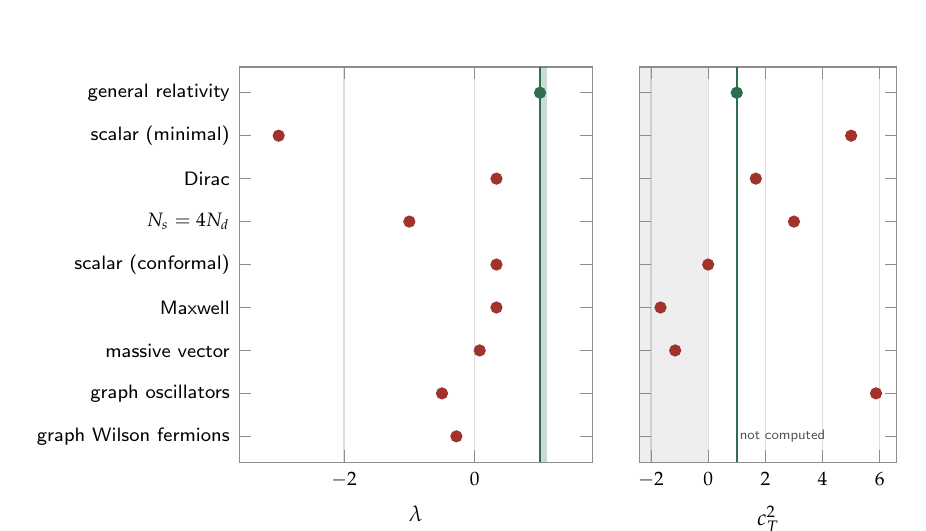
\begin{tikzpicture}
\begin{axis}[name=lam,width=0.50\textwidth,height=66mm,xmin=-3.6,xmax=1.8,ymin=0.4,ymax=9.6,y dir=reverse,
  ytick={1,...,9},yticklabels={general relativity,scalar (minimal),Dirac,$N_s=4N_d$,scalar (conformal),Maxwell,massive vector,graph oscillators,graph Wilson fermions},
  yticklabel style={font=\sffamily\scriptsize},xticklabel style={font=\sffamily\scriptsize},
  xlabel={$\lambda$},xlabel style={font=\sffamily\footnotesize},
  xmajorgrids,grid style={rulegray!30},axis line style={rulegray},tick style={rulegray},clip=true]
\fill[okgreen,opacity=0.25] (axis cs:1,0.4) rectangle (axis cs:1.1,9.6);
\draw[okgreen,line width=0.8pt] (axis cs:1,0.4)--(axis cs:1,9.6);
\addplot[only marks,mark=*,mark size=2pt,okgreen] coordinates {(1,1)};
\addplot[only marks,mark=*,mark size=2pt,badred] coordinates {(-3,2) (0.3333,3) (-1,4) (0.3333,5) (0.3333,6) (0.0769,7) (-0.5,8) (-0.28,9)};
\end{axis}
\begin{axis}[at={(lam.east)},anchor=west,xshift=6mm,width=0.40\textwidth,height=66mm,xmin=-2.4,xmax=6.6,ymin=0.4,ymax=9.6,y dir=reverse,
  ytick={1,...,9},yticklabels={},xticklabel style={font=\sffamily\scriptsize},
  xlabel={$c_T^2$},xlabel style={font=\sffamily\footnotesize},
  xmajorgrids,grid style={rulegray!30},axis line style={rulegray},tick style={rulegray},clip=true]
\fill[rulegray,opacity=0.15] (axis cs:-2.4,0.4) rectangle (axis cs:0,9.6);
\draw[okgreen,line width=0.8pt] (axis cs:1,0.4)--(axis cs:1,9.6);
\addplot[only marks,mark=*,mark size=2pt,okgreen] coordinates {(1,1)};
\addplot[only marks,mark=*,mark size=2pt,badred] coordinates {(5,2) (1.6667,3) (3,4) (0,5) (-1.6667,6) (-1.1538,7) (5.87,8)};
\node[font=\sffamily\tiny,text=rulegray!60!black] at (axis cs:2.6,9) {not computed};
\end{axis}
\end{tikzpicture}
\caption{The values of Table~\ref{tab:models}. Green: the window $0\le\lambda-1\lesssim0.1$ allowed by stability and observation, and $c_T^2=1$; the observational window for $c_T$ is far narrower than the line. Grey: $c_T^2<0$, a gradient instability of the tensor modes. No model of the table other than general relativity lies in either window.}\label{fig:models}
\end{figure}

The missing input can thus be stated in three equivalent ways: the total energy--momentum vanishes; the entanglement of small balls is stationary; the background is a summed-over variable rather than a parameter. The fixed-point argument above shows that none of these follows from the reconstruction theorems, Proposition~\ref{prop:nordstrom} excludes the scalar sector as a substitute, and Propositions~\ref{prop:shiftresponse} and~\ref{prop:nocancel} show that a model in which persistent nodes carry the cutoff leads, even with the principle, to a theory with a preferred foliation, Proposition~\ref{prop:lambda} shows that this theory has the wrong sign of $\lambda-1$, and by Section~\ref{sec:potential} its tensor modes do not propagate with the speed of the field.

For special field contents the leading non-covariant terms cancel, but for the fields considered the cancellation of all non-covariant terms, including those of the vacuum energy, implies that the induced action itself vanishes, at the orders $\Lambda^2$, $m^2\ln\Lambda$ and $m^2$ (Corollary~\ref{cor:vanish}). A model that yields Einstein's equation must therefore have a short-distance structure that does not single out a frame; within the class of node systems and fields considered in this paper, to second order in the perturbation of a flat slice, we have found none.

The parts of this conclusion do not have the same status. That the induced action of a node system is of Ho\v{r}ava type, and that $\lambda\le1$ whenever the Hamiltonian is linear in the shift, are proven (Propositions~\ref{prop:shiftresponse}--\ref{prop:lambda}). The statement on field contents rests on Proposition~\ref{prop:relations}, which is verified by computation on the listed fields and derived only for form fields at leading order (Remark~\ref{rem:reduced}). In the course of this work the conclusion on field contents changed whenever a further kind of field was included, first with scalar fields coupled to the curvature and then with massive vector fields, and another kind of field could change it again. We therefore regard the negative result as evidence within the computed class and not as a no-go theorem.

\paragraph{The vacuum term} The term $\rho_{\mathrm{vac}}\sim\varepsilon^{-2}$ is not forced by the construction; it depends on the field content.

\begin{proposition}[Field content]\label{prop:vacuum}
For $N_s$ minimally coupled scalar fields and $N_d$ Dirac fields with a common proper-time cutoff $\varepsilon$, to leading order in $m^2\varepsilon$,
\begin{equation}
\rho_{\mathrm{vac}}=-\frac{N_s-4N_d}{64\pi^2\varepsilon^2},\qquad M_{\mathrm{ind}}^2=\frac{N_s+2N_d}{96\pi^2\varepsilon}.
\end{equation}
For $N_s=4N_d$, equal numbers of bosonic and fermionic degrees of freedom, the quadratically divergent vacuum term cancels while $M_{\mathrm{ind}}^2=N_d/16\pi^2\varepsilon>0$.
\end{proposition}

\begin{proof}
The scalar contributes $-\tfrac12\int\frac{\dd s}{s}e^{-m^2s}\Tr e^{s\Delta}$ and the Dirac field $+\tfrac12\int\frac{\dd s}{s}e^{-m^2s}\Tr e^{-sD^2}$ with $D^2=-\nabla^2+\tfrac14R$ on four-component spinors, whose heat coefficients are $a_0=4$ and $a_1=4(\tfrac16-\tfrac14)R=-\tfrac13R$. The integrand is therefore $-\tfrac12(4\pi s)^{-2}\big[(N_s-4N_d)+sR\,(\tfrac{N_s}6+\tfrac{N_d}3)\big]$, and the claim follows as in Remark~\ref{rem:induced}.
\end{proof}

Both kinds of fields are minimally coupled, so Proposition~\ref{prop:principles} continues to hold, and both contribute to the entanglement with the same sign. The weight of the combined heat traces changes sign, which is the situation not excluded by Theorem~\ref{thm:nostat}. The terms of order $m^2/\varepsilon$ cancel under a second sum rule on the masses; a finite remainder of order $m^4$ is left, so the cosmological constant problem is reduced to its usual form, not solved.

\paragraph{Limits} Theorem~\ref{thm:nostat} shows that \eqref{eq:induced} without matter has no solution for a single scalar field: the trace of the left-hand side does not vanish. For non-minimally coupled fields the entanglement entropy and $A/4G_{\mathrm{ind}}$ differ \cite{Solodukhin}, and the two principles are no longer equivalent. Finally, (P2) is a statement about first-order variations around a maximally symmetric vacuum; the non-linear equation rests on (P1).

\section{Interpretation}\label{sec:reading}

\paragraph{Spatial reading} If $C_{ij}$ is the mutual information of subsystems in a state $\rho$, the nodes live on a spatial slice and $d$ is the spatial dimension. For $d=3$, \eqref{eq:heat} is a functional of the three-geometry: volume, integrated scalar curvature and the quadratic invariants. It has the form of the potential term of a Hamiltonian formulation; the kinetic term, built from extrinsic curvature, and four-dimensional covariance are not obtained. In this reading Corollary~\ref{cor:fixed} is too rigid, since Einstein three-manifolds have constant curvature. We regard this reading as the one supported by the construction.

\paragraph{Euclidean reading} If instead the nodes are cells of a four-dimensional Euclidean lattice and $C_{ij}$ is the classical mutual information of the Euclidean field measure, Proposition~\ref{prop:classical} applies, the correlations again decay as the square of the propagator, and the theorems of Section~\ref{sec:recon} hold with $d=4$. Then \eqref{eq:d4} is available, with the sign discussion of Remark~\ref{rem:coeff}. The price is that the four-dimensional geometry, including the Euclidean time direction, is part of the input, and operator algebras and modular structure play no role.

\section{Open problems}\label{sec:open}

\begin{enumerate}
\item \emph{Rates.} The bias $O(\xi^2)$ is proven for fixed simple eigenvalues (Theorem~\ref{thm:rate2}). Make it uniform in $k$ up to $\lambda_k\sim\xi^{-2}$, and extend it to multiple eigenvalues and to the eigenvectors. On a flat torus with the Gaussian profile the eigenvalues are controlled uniformly and with multiplicities, with the explicit bias $-\frac14\xi^2\lambda_k^2$ and a random error $C(\log N/N\xi^{d+2})^{1/2}\lambda_k^{(d+1)/2}$ (Theorem~\ref{thm:eigtorus}); this gives \eqref{eq:eigrate2} there when $N\xi_N^{3d}/\log N\to\infty$. With the comparison of the kernel in the mean over one index the random error becomes $C\frac{\delta'}\xi\lambda_k^{1/2}+C\sqrt{\log N/N}\,\lambda_k^{(d+2)/2}$, and \eqref{eq:eigrate2} holds when $N\xi_N^{\max(d+2,2d)}/\log N\to\infty$ (Theorem~\ref{thm:eigtorus-l1}; less often read than Theorem~\ref{thm:eigtorus}, see Table~\ref{tab:status}). The eigenspaces are controlled there in the Euclidean norm (Corollary~\ref{cor:eigspace}). Open: other manifolds and profiles, a random error without the term $\sqrt{\log N/N}\,\lambda_k^{(d+2)/2}$ that comes from the spectrum of the kernel matrix, and the eigenvectors in the supremum norm.
\item \emph{Heat trace.} Improve the relative error $O(\xi/\sqrt t)$ in \eqref{eq:tracerate} to $O(\xi^2/t)$ in the joint regime $N\to\infty$, $\xi_N\to0$. On a flat torus with the Gaussian profile this is proven, with the sharp coefficient $d(d+2)/8\tau$, almost surely for $N\xi_N^{d+6}/\log N\to\infty$ (Corollary~\ref{cor:kernel-trace}), by a comparison of the sampled walk with the population walk in the supremum norm; in probability for $N\xi_N^{d+4}/\log N\to\infty$ in dimensions one and two, by a second use of that comparison (Corollary~\ref{cor:secondstage}), and in every dimension when the second use is made in the mean over one index (Corollary~\ref{cor:secondstage-alld}); and in probability for $N\xi_N^{2d+6}/\log N\to\infty$ by a count of closed walks (Theorem~\ref{thm:jointpoly}). None of these proofs uses the eigenvalues. Known in addition: the coefficient $\beta\,d(d+2)/8\tau$ at the population level for other profiles (Theorems~\ref{thm:rate}, \ref{thm:profile}, \ref{thm:profileHS}); its removal by a correction or by the trace in discrete time (Theorem~\ref{thm:corrected}); the round sphere (Corollary~\ref{cor:sphere}); and the reduction of the general case to \eqref{eq:eigrate2} (Proposition~\ref{prop:ratereduction}), which is (1); and, at a fixed kernel scale, the term of the order $1/N$ of the mean of $\Tr P^k$, most of which is due to the self-loops (Proposition~\ref{prop:bias}), and its variance of the order $1/N^2$ (Proposition~\ref{prop:variance}). Open: smaller kernel scales, for which Remarks~\ref{rem:bias}(v) and~\ref{rem:variance}(v) state a conjecture, other manifolds in the joint regime, and the points of Remark~\ref{rem:rateopen}.
\item \emph{Independent verification.} None of the proofs has been checked by a second reader. The comparison of Dirichlet forms (Appendix~\ref{app:dirichlet}) and Sections~\ref{sec:scalar}--\ref{sec:matter} are the parts where an error would have the largest consequences. Appendix~\ref{app:heat} has been read by further sessions of the AI system that wrote it, each started without knowledge of the earlier assessments and instructed to find errors. They found one error in a statement, a missing hypothesis in Theorem~\ref{thm:profile} with an explicit counterexample to the earlier wording, which is corrected, and a number of gaps of presentation, which are closed; they did not check the cited results. This does not replace a reader.
\item \emph{End-to-end statement.} Rewrite the proofs of Theorem~\ref{thm:window}(ii), (iii) line by line; extend Theorem~\ref{thm:e2e} to the borderline $\xi_0\sim\xi$, to several modes per node, to nodes that are not sampled independently, and to noisy data.
\item \emph{Lapse reconstruction.} Build an estimator of $\Omega$ from the cross-ratios with a convergence statement, beyond leading order in $1/\bar m\hat r$.
\item \emph{Interacting systems.} Extend Theorem~\ref{thm:cluster2} to continuous-variable nodes, that is, bound the non-Gaussianity $D(\rho_{AB}\|\rho^G_{AB})$ of distant pairs; verify the hypotheses of the extremality lemma of \cite{WGC} in infinite dimensions; and control the direction dependence of the logarithmic drift in Corollary~\ref{cor:gapped}.
\item \emph{Time.} Prove the $N$-point version of Proposition~\ref{prop:dotL}, and control the corrections to the profile form in Theorem~\ref{thm:xray}(b). Proposition~\ref{prop:modular} recovers the Hamiltonian for states of the vacuum type; a quantitative version on curved backgrounds and for the lattice, and a characterisation of the states for which the modular flow of small regions is geometric, are open.
\item \emph{The principle and the cutoff.} A model in which the background is a variable and (P1) or (P2) can be proven must avoid the obstruction of Propositions~\ref{prop:shiftresponse} and~\ref{prop:nocancel}: its short-distance structure must not single out a frame. Candidates outside the present framework are a cutoff that depends on the background, and a statistical discreteness of spacetime rather than of space \cite{BHS}. The third possibility, to accept the preferred foliation, is excluded by Proposition~\ref{prop:lambda} and by the tensor speed \eqref{eq:cT}. Tables~\ref{tab:models} and~\ref{tab:species} list the values for scalar, Dirac and Maxwell fields and for the kernel graph. 

By Corollary~\ref{cor:content} the leading non-covariant terms cancel for special field contents, but not together with the vacuum energy unless the induced action vanishes at the order $\Lambda^2$. At the next order the logarithmic terms are covariant, but the finite terms of order $m^2$ are not, and they force $\lambda<1$ for every monotone cutoff profile unless massive vector fields are present; with them the non-covariant terms of the induced action can be cancelled, but together with the vacuum energy of the order $m^2\Lambda^2$ only if the induced action vanishes (Corollary~\ref{cor:vanish}). Open in this direction:
\begin{itemize}
\item a derivation of \eqref{eq:reduced} that includes the Dirac field, the coupling $\zeta$ and the finite parts $a_{\mathrm f}$, $\ell_{\mathrm f}$;
\item the finite parts in dimensions other than three;
\item terms beyond second order;
\item lattice and graph dispersions at this order;
\item fields of spin $\tfrac32$ and $2$;
\item terms of higher order in the shift and mixed terms;
\item the validity of the two-term expansion for sharp cutoffs;
\item a Dirac operator on the kernel graph without given coordinates, and its curvature term;
\item a proof of the sampling corrections to \eqref{eq:graphE} and \eqref{eq:graphlong}, which are so far only checked numerically.
\end{itemize}
The vacuum term is reduced to the usual fine-tuning problem (Proposition~\ref{prop:vacuum}).
\end{enumerate}

\section{Changes with respect to version 2}\label{sec:changes}

\begin{itemize}
\item Assumption~2.3 (approximate isometry) is replaced by Assumption~\ref{ass:profile}; the former is false for free fields (Corollary~\ref{cor:drift}).
\item Proposition~2.6 and Appendix~B (Bisognano--Wichmann argument) are withdrawn. The boost parameter was misidentified with a proper distance, the theorem was applied outside its hypotheses, and the two bounds had different exponents. Theorems~\ref{thm:decay} and~\ref{thm:curved} take their place.
\item Spectral convergence is proven (Theorems~\ref{thm:eig}, \ref{thm:evec}) instead of assumed.
\item The spectral embedding is weighted by $\pi$ (Theorem~\ref{thm:isometry}).
\item The functional $\Tr e^{-t\Lc}$ at $t=\xi^2/2$ is replaced by the subtracted trace in the regime $\xi^2\ll t$; the scale of the curvature coefficients is $t$, not $\xi$ (Theorems~\ref{thm:poisson}, \ref{thm:trace}).
\item The claim of a four-dimensional Einstein--Hilbert action from spatial correlations is withdrawn (Section~\ref{sec:reading}); the topological term $\chi(\M)/90$ is added to \eqref{eq:d4}; the sign of the curvature term is discussed (Remark~\ref{rem:coeff}).
\item The variational ansatz and the response functional of the former Section~4 are withdrawn and replaced by Section~\ref{sec:dyn}; the scalar degree of freedom is identified in Section~\ref{sec:scalar}.
\item The reconstruction is closed end to end for the free field (Section~\ref{sec:window}, Theorem~\ref{thm:e2e}, Appendix~\ref{app:e2e}); the earlier outline proofs for geodesic modes are replaced by complete ones.
\item Sections~\ref{sec:scalar}--\ref{sec:matter} are new. They contain the negative results on dynamics: a scalar response gives Nordstr\"om's theory (Proposition~\ref{prop:nordstrom}), and node systems induce a theory with a preferred foliation that is not viable (Propositions~\ref{prop:shiftresponse}--\ref{prop:lambda}).
\item Related work on the metric from field correlators \cite{SAK,Kempf21,PercheMM}, on graph Laplacians with general kernels \cite{HAvL,THJ} and on induced actions of Ho\v{r}ava--Lifshitz type \cite{NS10,DSS,LMP} is cited and the present results are delimited against it (Introduction, Section~\ref{sec:nodecov}); the conclusion on field contents is stated as evidence within the computed class (Section~\ref{sec:nodesummary}).
\item Appendix~\ref{app:heat} extends the two theorems on the heat trace, including the rate $\xi^2/t$ at the population level, its correction, other profiles, the limit $N\to\infty$ at fixed $\xi$ (Theorems~\ref{thm:rate}--\ref{thm:fixedxi}), a joint regime (Theorem~\ref{thm:jointpoly}), an estimate of the kernel of the sampled walk that is uniform in the number of steps (Lemma~\ref{lem:consistency}, Theorem~\ref{thm:kernel}, Corollaries~\ref{cor:kernel-trace}, \ref{cor:kernel-corrected}, \ref{cor:kernel-noloops}), with it a second stage for the trace (Corollary~\ref{cor:secondstage}) and a uniform estimate of the eigenvalues on a flat torus with its consequences for eigenspaces and eigenvectors (Theorem~\ref{thm:eigtorus}, Corollaries~\ref{cor:eigspace}, \ref{cor:deloc}), a comparison of the kernel in the mean over one index with a second stage in every dimension and a second estimate of the eigenvalues (Lemma~\ref{lem:kernel-l1}, Proposition~\ref{prop:reduction-alld}, Corollary~\ref{cor:secondstage-alld}, Theorem~\ref{thm:eigtorus-l1}), and the bias and the variance of the sampled trace at a fixed kernel scale (Propositions~\ref{prop:bias}, \ref{prop:variance}), and the finite parts of these and of the statements on field contents are checked with the proof assistant Lean (Remark~\ref{rem:lean}).
\end{itemize}


\appendix

\section{Proof of Theorem~\ref{thm:LB}}\label{app:LB}

\begin{lemma}\label{lem:G}
For $\varphi\in C^4(\M)$, uniformly in $x$,
\begin{equation}\label{eq:G}
(G_\xi\varphi)(x)\equiv\int K_\xi(x,y)\varphi(y)\,\dd V(y)=m_0\xi^d\Big[\varphi+\frac{c_h\xi^2}{2}\Big(\Delta_g\varphi-\frac R3\varphi\Big)+O(\xi^4)\Big](x).
\end{equation}
\end{lemma}

\begin{proof}
Fix $\rho$ smaller than the injectivity radius. Outside the ball $B(x,\rho)$ we have $K_\xi\le Ae^{-\rho/\xi}$, so that part is smaller than any power of $\xi$. Inside, put $y=\exp_x(\xi u)$. In normal coordinates $d_g(x,y)=\xi|u|$ exactly and $\dd V=\xi^d\big[1-\tfrac{\xi^2}{6}\Ric_{\alpha\beta}u^\alpha u^\beta+\xi^3c_3(u)+O(\xi^4|u|^4)\big]\dd u$ with $c_3$ cubic. Expanding $\varphi(\exp_x(\xi u))$ to third order with remainder $O(\xi^4|u|^4)$ and extending the integral to $\R^d$, again at exponentially small cost, we integrate against $h(|u|)\,\dd u$. Odd terms vanish by radial symmetry and $\int h(|u|)u^\alpha u^\beta\,\dd u=m_2\delta^{\alpha\beta}$. The trace of the Hessian in normal coordinates is $\Delta_g\varphi$ and that of $\Ric$ is $R$. Compactness makes all bounds uniform.
\end{proof}

\begin{proof}[Proof of Theorem~\ref{thm:LB}]
Let $\beta=\tfrac{c_h}{2}\big(\Delta_g\mu/\mu-R/3\big)\in C^4$. Lemma~\ref{lem:G} with $\varphi=\mu$ gives $q_\xi=m_0\xi^d\mu\,[1+\xi^2\beta+\xi^4r_\xi]$ with $r_\xi$ bounded. Hence $f\mu/q_\xi=(m_0\xi^d)^{-1}[f-\xi^2\beta f+\xi^4\tilde r_\xi]$ with $\tilde r_\xi$ bounded, and since $G_\xi$ is positivity preserving with $G_\xi1=O(\xi^d)$, the last term contributes $O(\xi^4)$. Applying the lemma to $f-\xi^2\beta f\in C^4$,
\begin{equation}
\begin{split}
q_\xi(x)\int W_\xi(x,y)f(y)\mu(y)\,\dd V(y)&=G_\xi\Big[\frac{f\mu}{q_\xi}\Big](x)\\
&=f+\xi^2\Big[\frac{c_h}{2}\Delta_gf+\Big(-\frac{c_h}{6}R-\beta\Big)f\Big]+O(\xi^4).
\end{split}
\end{equation}
The same expression with $f\equiv1$ is the denominator, $1+\xi^2(-\tfrac{c_h}{6}R-\beta)+O(\xi^4)$. In the quotient all terms of the form $\xi^2\cdot(\text{function})\cdot f$ cancel, so $P_\xi f=f+\tfrac{c_h\xi^2}{2}\Delta_gf+O(\xi^4)$.
\end{proof}

\section{Dirichlet-form comparison}\label{app:dirichlet}

This appendix proves Theorems~\ref{thm:eig} and~\ref{thm:evec}. The deterministic part (Proposition~\ref{prop:det}) follows the method of \cite{BIK}; the extension from ball graphs to a monotone profile is done by a layer-cake decomposition. Throughout $d\ge2$, $r_0\in(0,\mathrm{inj}(\M))$ is fixed, $\nu_d$ is the volume of the unit ball of $\R^d$, $\|\cdot\|$ is the norm of $L^2(\M,\dd V_g)$, and $c,C$ denote positive constants that depend only on $(\M,g)$, $\mu$ and $h$ and may change from line to line. In normal coordinates at $x$ the volume element is $J_x(v)\,\dd v$ with
\begin{equation}\label{eq:J}
|J_x(v)-1|\le C|v|^2\qquad(|v|\le r_0).
\end{equation}

\subsection{Layer-cake form and two lemmas}

Changing $h$ on a countable set alters neither its moments nor, almost surely, any $K_{ij}$, because the law of $d_g(x_i,x_j)$ has no atoms. We may therefore assume that $h$ is right-continuous. Then $h(s)=\nu_h((s,\infty))$ for a positive measure $\nu_h$ on $(0,\infty)$, and
\begin{equation}\label{eq:moments}
M_p\equiv\int t^p\,\nu_h(\dd t)=p\int_0^\infty s^{p-1}h(s)\,\dd s<\infty\quad(p>0),\qquad m_2=\frac{\nu_d}{d+2}\,M_{d+2}.
\end{equation}
For $f\in L^2(\M)$ let
\begin{equation}
E_r(f)=\iint_{d_g(x,y)<r}\big(f(x)-f(y)\big)^2\,\dd V(x)\,\dd V(y)\quad(r>0),\qquad E_r(f)=0\quad(r\le0).
\end{equation}
Since $(\rho+b)_+<t\xi$ is equivalent to $\rho<t\xi-b$ for $t>0$, we have for every $b\in\R$
\begin{equation}\label{eq:layer}
\iint h\Big(\frac{(d_g(x,y)+b)_+}{\xi}\Big)\big(f(x)-f(y)\big)^2\,\dd V\,\dd V=\int\nu_h(\dd t)\,E_{t\xi-b}(f).
\end{equation}

\begin{lemma}\label{lem:Er}
For $f\in H^1(\M)$ and $0<r\le r_0$,
$\displaystyle E_r(f)\le(1+Cr^2)\,\frac{\nu_d\,r^{d+2}}{d+2}\,\|\dd f\|^2 .$
\end{lemma}

\begin{proof}
Let $f$ be smooth; the general case follows by density. For $y=\exp_x(v)$, $f(y)-f(x)=\int_0^1\dd f(\dot\gamma_{x,v}(s))\,\dd s$ along the geodesic $\gamma_{x,v}(s)=\exp_x(sv)$, so $(f(y)-f(x))^2\le\int_0^1\dd f(\dot\gamma_{x,v}(s))^2\,\dd s$. With \eqref{eq:J},
\[
E_r(f)\le(1+Cr^2)\int_0^1\dd s\int_{\{(x,v)\in T\M:\,|v|<r\}}\dd f\big(\Phi_s(x,v)\big)^2\,\dd V(x)\,\dd v ,
\]
where $\Phi_s(x,v)=\dot\gamma_{x,v}(s)$ is the geodesic flow. It preserves the Liouville measure $\dd V\,\dd v$ and the set $\{|v|<r\}$, so the inner integral equals $\int\dd V(x)\int_{|v|<r}\dd f_x(v)^2\,\dd v=\tfrac{\nu_dr^{d+2}}{d+2}\|\dd f\|^2$.
\end{proof}

For $0<r\le r_0$ let $\psi(s)=\tfrac{d+2}{2\nu_d}(1-s^2)_+$, so that $\int_{\R^d}\psi(|u|)\,\dd u=1$, and define the smoothing operator
\begin{equation}
(\Lambda_rf)(x)=\frac{1}{\theta_r(x)\,r^d}\int\psi\Big(\frac{d_g(x,y)}{r}\Big)f(y)\,\dd V(y),\qquad \theta_r(x)=\frac1{r^d}\int\psi\Big(\frac{d_g(x,y)}{r}\Big)\dd V(y).
\end{equation}
By \eqref{eq:J}, $|\theta_r-1|\le Cr^2$ and $|\dd\theta_r|\le Cr$.

\begin{lemma}\label{lem:smooth}
For bounded measurable $f$ and $0<r\le r_0$, $\Lambda_rf$ is Lipschitz and
\begin{equation}
\|\Lambda_rf-f\|^2\le\frac{C}{r^d}\,E_r(f),\qquad \|\dd\Lambda_rf\|^2\le(1+Cr^2)\,\frac{d+2}{\nu_d\,r^{d+2}}\,E_r(f).
\end{equation}
\end{lemma}

\begin{proof}
Since $\Lambda_r1=1$, $(\Lambda_rf-f)(x)=\theta_r^{-1}r^{-d}\int\psi(d_g(x,y)/r)(f(y)-f(x))\,\dd V(y)$. The Cauchy--Schwarz inequality and $\int\psi(d_g/r)^2\dd V\le Cr^d$ give $|\Lambda_rf-f|^2(x)\le Cr^{-d}\int_{B(x,r)}(f(y)-f(x))^2\dd V(y)$; integrate over $x$. For the gradient, differentiate the same identity at $x$:
\[
\dd(\Lambda_rf)(x)=\frac{1}{\theta_rr^d}\int\dd_x\psi\Big(\frac{d_g(x,y)}{r}\Big)\big(f(y)-f(x)\big)\,\dd V(y)-\frac{\dd\theta_r}{\theta_r}\,(\Lambda_rf-f)(x)\equiv A_1+A_2 .
\]
With $y=\exp_x(v)$, the gradient of $x\mapsto\psi(d_g(x,y)/r)$ is $\tfrac{d+2}{\nu_dr^2}\,v$ for $|v|<r$. For a unit vector $w$, by Cauchy--Schwarz and $\int_{|v|<r}\langle v,w\rangle^2J_x(v)\,\dd v\le(1+Cr^2)\tfrac{\nu_dr^{d+2}}{d+2}$,
\[
\langle A_1,w\rangle^2\le(1+Cr^2)\,\frac{d+2}{\nu_dr^{d+2}}\int_{B(x,r)}\big(f(y)-f(x)\big)^2\,\dd V(y).
\]
Integration over $x$ bounds $\|A_1\|^2$ by the right-hand side of the claim. The term $A_2$ is smaller by a factor $Cr^2$, since $\|A_2\|\le Cr\|\Lambda_rf-f\|\le Cr^{1-d/2}E_r(f)^{1/2}$.
\end{proof}

\subsection{The deterministic comparison}

Let $\M=\bigsqcup_{i=1}^NU_i$ be a measurable partition and $x_1,\dots,x_N\in\M$ with $U_i\subset B(x_i,\varepsilon)$ and $v_i=\Vol(U_i)>0$. On $\R^N$ define
\begin{equation}\label{eq:Gamma}
\|u\|_\Gamma^2=\sum_iv_iu_i^2,\qquad \mathcal E_\Gamma(u)=\frac{1}{m_2\,\xi^{d+2}}\sum_{i,j}v_iv_j\,h\Big(\frac{d_g(x_i,x_j)}{\xi}\Big)(u_i-u_j)^2 ,
\end{equation}
and let $\lambda_0(\Gamma)\le\dots\le\lambda_{N-1}(\Gamma)$ be the min--max values of $\mathcal E_\Gamma/\|\cdot\|_\Gamma^2$. Let $(Pf)_i=v_i^{-1}\int_{U_i}f\,\dd V$ and $P^*u=\sum_iu_i\mathbf 1_{U_i}$, so that $\|P^*u\|=\|u\|_\Gamma$ and $\|Pf\|_\Gamma\le\|f\|$.

\begin{proposition}\label{prop:det}
There are constants $c,C$ such that for $\xi\le c$ and $\varepsilon\le c\,\xi$, with $T_\xi=2\ln(1/\xi)$ and $\kappa_\xi=\xi^{-d-2}e^{-r_0/2\xi}$:
\begin{enumerate}[label=\textup{(\alph*)}]
\item for $f\in H^1(\M)$: $\ \mathcal E_\Gamma(Pf)\le\big(1+C(\varepsilon/\xi+\xi^2)\big)\|\dd f\|^2+C\kappa_\xi\|f\|^2$ and $\|f-P^*Pf\|\le C\varepsilon\|\dd f\|$;
\item there is a linear map $\mathcal I:\R^N\to H^1(\M)$ with
$\|\dd\,\mathcal Iu\|^2\le\big(1+C(\varepsilon/\xi+\xi)\big)\mathcal E_\Gamma(u)$ and $\|\mathcal Iu-P^*u\|\le C\,\xi\,\mathcal E_\Gamma(u)^{1/2}$.
\end{enumerate}
Consequently, for $0\le k\le N-1$,
\begin{align}
\lambda_k(\Gamma)&\le\frac{\big(1+C(\varepsilon/\xi+\xi^2)\big)\lambda_k+C\kappa_\xi}{\big(1-C\varepsilon\sqrt{\lambda_k}\big)^2}&&\text{if }C\varepsilon\sqrt{\lambda_k}<1,\label{eq:U}\\
\lambda_k&\le\frac{\big(1+C(\varepsilon/\xi+\xi)\big)\lambda_k(\Gamma)}{\big(1-C\xi\sqrt{\lambda_k(\Gamma)}\big)^2}&&\text{if }C\xi\sqrt{\lambda_k(\Gamma)}<1.\label{eq:Lo}
\end{align}
\end{proposition}

\begin{proof}
\emph{(a)} By Jensen's inequality $((Pf)_i-(Pf)_j)^2\le(v_iv_j)^{-1}\int_{U_i}\int_{U_j}(f(x)-f(y))^2$. For $x\in U_i$, $y\in U_j$ we have $d_g(x_i,x_j)\ge(d_g(x,y)-2\varepsilon)_+$, and $h$ is nonincreasing, so by \eqref{eq:layer} with $b=-2\varepsilon$
\[
m_2\xi^{d+2}\,\mathcal E_\Gamma(Pf)\le\int\nu_h(\dd t)\,E_{t\xi+2\varepsilon}(f).
\]
For $t\xi+2\varepsilon\le r_0$ we use Lemma~\ref{lem:Er}; for larger $t$ the trivial bound $E_r(f)\le4\Vol(\M)\|f\|^2$, with $\nu_h(\{t\xi+2\varepsilon>r_0\})=h((r_0-2\varepsilon)/\xi)\le Ae^{-r_0/2\xi}$. Writing $\eta=2\varepsilon/\xi\le1$ and using $(t+\eta)^{d+2}\le t^{d+2}+(d+2)\eta(t+1)^{d+1}$,
\[
\int\nu_h(\dd t)\,(t+\eta)^{d+2}\big(1+C\xi^2(t+\eta)^2\big)\le M_{d+2}+C\eta+C\xi^2 ,
\]
because $\int(t+1)^p\nu_h(\dd t)<\infty$ for all $p$ by \eqref{eq:moments}. Dividing by $m_2\xi^{d+2}=\tfrac{\nu_d}{d+2}\xi^{d+2}M_{d+2}$ gives the first claim. For the second, $\|f-P^*Pf\|^2=\sum_i(2v_i)^{-1}\int_{U_i}\int_{U_i}(f(x)-f(y))^2$. For $x,y\in U_i$ and $z\in B(x_i,\varepsilon)$ we have $(f(x)-f(y))^2\le2(f(x)-f(z))^2+2(f(z)-f(y))^2$; averaging over $z$ and using $B(x_i,\varepsilon)\subset B(x,2\varepsilon)$ for $x\in U_i$,
\[
\|f-P^*Pf\|^2\le\frac{2}{\min_i\Vol B(x_i,\varepsilon)}\,E_{2\varepsilon}(f)\le C\varepsilon^2\|\dd f\|^2
\]
by Lemma~\ref{lem:Er} and $\Vol B(x_i,\varepsilon)\ge c\,\varepsilon^d$.

\emph{(b)} For $x\in U_i$, $y\in U_j$ we have $d_g(x_i,x_j)\le d_g(x,y)+2\varepsilon$, hence by \eqref{eq:layer} with $b=2\varepsilon$ and $r_t=t\xi-2\varepsilon$,
\begin{equation}\label{eq:lowform}
m_2\xi^{d+2}\,\mathcal E_\Gamma(u)\ge\int\nu_h(\dd t)\,E_{r_t}(P^*u).
\end{equation}
Let $Z=\int_{\eta<t\le T_\xi}\nu_h(\dd t)\,r_t^{d+2}$ and define, with the probability measure $\varpi(\dd t)=Z^{-1}r_t^{d+2}\mathbf 1_{\{\eta<t\le T_\xi\}}\nu_h(\dd t)$,
\[
\mathcal Iu=\int\varpi(\dd t)\,\Lambda_{r_t}P^*u .
\]
Here $r_t\le\xi T_\xi\le r_0$ for small $\xi$. By convexity of the norm, Jensen's inequality, Lemma~\ref{lem:smooth} and \eqref{eq:lowform},
\[
\begin{split}
\|\dd\,\mathcal Iu\|^2\le\int\varpi(\dd t)\,\|\dd\Lambda_{r_t}P^*u\|^2&\le(1+C\xi^2T_\xi^2)\,\frac{d+2}{\nu_dZ}\int\nu_h(\dd t)\,E_{r_t}(P^*u)\\
&\le(1+C\xi^2T_\xi^2)\,\frac{\xi^{d+2}M_{d+2}}{Z}\,\mathcal E_\Gamma(u).
\end{split}
\]
From $(t-\eta)_+^{d+2}\ge t^{d+2}-(d+2)\eta\,t^{d+1}$ and $\int_{t>T}t^{d+2}\nu_h(\dd t)=T^{d+2}h(T)+(d+2)\int_T^\infty s^{d+1}h(s)\,\dd s\le CT^{d+2}e^{-T}$,
\[
\xi^{-d-2}Z\ge M_{d+2}-(d+2)\eta M_{d+1}-CT_\xi^{d+2}\xi^2\ge M_{d+2}\,\big(1-C(\varepsilon/\xi+\xi)\big),
\]
which proves the first inequality of (b). For the second, Lemma~\ref{lem:smooth} gives $\|\Lambda_rf-f\|\le C\,r\,(r^{-d-2}E_r(f))^{1/2}$, and the Cauchy--Schwarz inequality with respect to $\varpi$ yields
\[
\begin{split}
\|\mathcal Iu-P^*u\|^2&\le C\int\varpi(\dd t)\,r_t^2\;\int\varpi(\dd t)\,\frac{E_{r_t}(P^*u)}{r_t^{d+2}}\\
&\le C\,\frac{\xi^{d+4}M_{d+4}}{Z}\cdot\frac{m_2\,\xi^{d+2}}{Z}\,\mathcal E_\Gamma(u)\le C\,\xi^2\,\mathcal E_\Gamma(u),
\end{split}
\]
because $\int\varpi(\dd t)\,r_t^2=Z^{-1}\int r_t^{d+4}\nu_h(\dd t)\le Z^{-1}\xi^{d+4}M_{d+4}$, the weight $r_t^{d+2}$ cancels in the second factor, and $Z\ge c\,\xi^{d+2}$.

\emph{Eigenvalues.} Let $L$ be the span of the first $k+1$ eigenfunctions of $-\Delta_g$, so $\|\dd f\|^2\le\lambda_k\|f\|^2$ on $L$. By (a), $\|Pf\|_\Gamma=\|P^*Pf\|\ge(1-C\varepsilon\sqrt{\lambda_k})\|f\|$, so $P$ is injective on $L$ and \eqref{eq:U} follows from the min--max principle applied to $P(L)$. For \eqref{eq:Lo} let $L_\Gamma$ be the span of the first $k+1$ eigenvectors of $\Gamma$; on it $\mathcal E_\Gamma(u)\le\lambda_k(\Gamma)\|u\|_\Gamma^2$, so by (b) $\|\mathcal Iu\|\ge\|u\|_\Gamma(1-C\xi\sqrt{\lambda_k(\Gamma)})$, and the min--max principle is applied to $\mathcal I(L_\Gamma)$.
\end{proof}

\subsection{Random weights and proof of Theorem~\ref{thm:eig}}

\begin{lemma}\label{lem:weights}
Let $a_i=1/(N\mu(x_i))$ and $\delta_N=\xi^2+\sqrt{\log N/(N\xi^d)}$. If $\xi\le c$ and $N\xi^d\ge C\log N$, then with probability at least $1-CN^{-2}$, for all $i,j$,
\begin{equation}\label{eq:weights}
W_{ij}=\frac{N^2a_ia_jK_{ij}}{m_0^2\,\xi^{2d}}\,(1+\theta_{ij}),\qquad D_i=\frac{N^2a_i}{m_0\,\xi^d}\,(1+\theta_i),\qquad|\theta_{ij}|,|\theta_i|\le C\delta_N .
\end{equation}
\end{lemma}

\begin{proof}
Conditionally on $x_i$, the variables $K(x_i,x_k)$, $k\ne i$, are independent, bounded by $A$, with mean $q_\xi(x_i)=m_0\xi^d\mu(x_i)(1+O(\xi^2))$ by Lemma~\ref{lem:G} and variance at most $C\xi^d$. Bernstein's inequality and a union bound give $q_i=m_0\xi^d\mu(x_i)(1+O(\delta_N))$ for all $i$ with probability $1-CN^{-2}$; the self-term $K_{ii}/N$ is of relative order $1/(N\xi^d)\le\delta_N$. This yields the formula for $W_{ij}=K_{ij}/(q_iq_j)$. The same argument applied to $\sum_kK(x_i,x_k)/(N\mu(x_k))$, whose conditional mean is $\int K_\xi(x_i,y)\,\dd V(y)=m_0\xi^d(1+O(\xi^2))$, gives the formula for $D_i=q_i^{-1}\sum_jK_{ij}/q_j$.
\end{proof}

\begin{lemma}\label{lem:traces}
On the event of Lemma~\ref{lem:weights}, $\ \Tr P\le C\xi^{-d}$ and $\Tr P^2=\Tr S^2\le C\xi^{-d}$.
\end{lemma}

\begin{proof}
By \eqref{eq:weights}, $P_{ij}=W_{ij}/D_i=a_jK_{ij}(m_0\xi^d)^{-1}(1+O(\delta_N))$. Hence $\Tr P\le C\xi^{-d}\sum_ia_i\le C\xi^{-d}$, and, using $K_{ij}\le A$ and $\sum_ja_jK_{ij}\le C\xi^d$ from the proof of Lemma~\ref{lem:weights},
$\Tr P^2=\sum_{i,j}P_{ij}P_{ji}\le C\xi^{-2d}\sum_ia_i\sum_ja_jK_{ij}^2\le C\xi^{-d}$.
\end{proof}

\begin{proof}[Proof of Theorem~\ref{thm:eig}]
Work on the intersection of the events of Lemmas~\ref{lem:transport} and~\ref{lem:weights}. Let $U_i=T^{-1}(x_i)$ and $\varepsilon=C_T\varepsilon_N$. Since $\mu(U_i)=1/N$ and $\mu$ is Lipschitz, $v_i=\Vol(U_i)=a_i(1+O(\varepsilon))$. With $s_N=m_0\xi^d/N^2$ put
\begin{equation}\label{eq:Nforms}
\|u\|_N^2=s_N\sum_iD_iu_i^2,\qquad \mathcal E_N(u)=\frac{s_N}{c_h\xi^2}\sum_{i,j}W_{ij}(u_i-u_j)^2,
\end{equation}
so that $R_N=\mathcal E_N/\|\cdot\|_N^2$. By \eqref{eq:weights}, $c_hm_0=m_2$ and \eqref{eq:Gamma}, for all $u$
\begin{equation}\label{eq:twosided}
(1-\bar\delta)\|u\|_\Gamma^2\le\|u\|_N^2\le(1+\bar\delta)\|u\|_\Gamma^2,\qquad(1-\bar\delta)\,\mathcal E_\Gamma(u)\le\mathcal E_N(u)\le(1+\bar\delta)\,\mathcal E_\Gamma(u),
\end{equation}
with $\bar\delta=C(\delta_N+\varepsilon)$. Since $d\ge2$ and $\varepsilon_N\le\xi$, we have $\sqrt{\log N/(N\xi^d)}\le(\varepsilon_N/\xi)^{d/2}\le\varepsilon_N/\xi$, so $\bar\delta\le C(\varepsilon_N/\xi+\xi)$, and the condition $N\xi^d\ge C\log N$ follows from $\varepsilon_N\le c\,\xi$. By min--max, $(1-C\bar\delta)\lambda_k(\Gamma)\le\lambda_k^N\le(1+C\bar\delta)\lambda_k(\Gamma)$ for all $k$.

(i) Let $\xi\sqrt{\lambda_k}\le c$. Then $C\varepsilon\sqrt{\lambda_k}\le\tfrac12$, and \eqref{eq:U} with $\kappa_\xi\le\xi\lambda_1$ gives $\lambda_k^N\le\lambda_k\,(1+C(\varepsilon_N/\xi+\xi+\varepsilon\sqrt{\lambda_k}))$. In particular $\lambda_k(\Gamma)\le4\lambda_k$, so $C\xi\sqrt{\lambda_k(\Gamma)}\le\tfrac12$ if $c$ is small, and \eqref{eq:Lo} gives $\lambda_k\le\lambda_k^N\,(1+C(\varepsilon_N/\xi+\xi+\xi\sqrt{\lambda_k}))$. Together these are \eqref{eq:eigrate}.

(ii) If $C\xi\sqrt{\lambda_k(\Gamma)}\ge\tfrac12$, then $\lambda_k(\Gamma)\ge c\,\xi^{-2}$. Otherwise \eqref{eq:Lo} gives $\lambda_k\le8\lambda_k(\Gamma)$. In both cases \eqref{eq:eiglow} follows from $\lambda_k^N\ge\tfrac12\lambda_k(\Gamma)$.

The last statement follows from the Borel--Cantelli lemma.
\end{proof}

\subsection{Eigenvectors}

\begin{lemma}\label{lem:kyfan}
Let $\mathfrak a(f)=\|\dd f\|^2$ on $H^1(\M)$, let $Q_j$ be the orthogonal projection of $L^2(\M)$ onto the span of $\psi_0,\dots,\psi_j$, and assume $\lambda_j<\lambda_{j+1}$. Let $L\subset H^1(\M)$ be a subspace of dimension $j+1$ with orthogonal projection $\Pi_L$ and orthonormal basis $e_0,\dots,e_j$. Then
\begin{equation}
\|(1-Q_j)\Pi_L\|_{\mathrm{HS}}^2=\|Q_j(1-\Pi_L)\|_{\mathrm{HS}}^2\le\frac{\sum_{i\le j}\mathfrak a(e_i)-\sum_{i\le j}\lambda_i}{\lambda_{j+1}-\lambda_j}.
\end{equation}
\end{lemma}

\begin{proof}
Let $p_n=\|\Pi_L\psi_n\|^2\in[0,1]$. Then $\sum_np_n=j+1$ and $\sum_i\mathfrak a(e_i)=\sum_n\lambda_np_n$. Since $\sum_{n>j}p_n=\sum_{n\le j}(1-p_n)$,
\[
\sum_n\lambda_np_n-\sum_{n\le j}\lambda_n=\sum_{n>j}\lambda_np_n-\sum_{n\le j}\lambda_n(1-p_n)\ge(\lambda_{j+1}-\lambda_j)\sum_{n>j}p_n ,
\]
and $\sum_{n>j}p_n=\Tr((1-Q_j)\Pi_L)=\|(1-Q_j)\Pi_L\|_{\mathrm{HS}}^2$. The first equality of the lemma holds because $Q_j$ and $\Pi_L$ have the same rank.
\end{proof}

\begin{proof}[Proof of Theorem~\ref{thm:evec}]
We work on the event of Theorem~\ref{thm:eig}, for $N$ large, and write $\mathrm{err}_N=\varepsilon_N/\xi_N+\xi_N$. Let $w_0,\dots,w_{N-1}$ be eigenvectors for the Rayleigh quotient $R_N$, orthonormal for $\|\cdot\|_N$ of \eqref{eq:Nforms}, and $\mathcal W_j=\operatorname{span}(w_0,\dots,w_j)$. Fix $j\le k$. For $u\in\mathcal W_j$, \eqref{eq:twosided} gives $\mathcal E_\Gamma(u)\le(1+C\bar\delta)\lambda_j^N\|u\|_\Gamma^2$, so by Proposition~\ref{prop:det}(b) and \eqref{eq:twosided},
\begin{equation}\label{eq:quasiiso}
\big|\|\mathcal Iu\|^2-\|u\|_N^2\big|\le\vartheta\,\|u\|_N^2,\qquad \|\dd\,\mathcal Iu\|^2\le(1+C\,\mathrm{err}_N)\,\mathcal E_N(u),
\end{equation}
with $\vartheta\le C_k\,\mathrm{err}_N$. By polarisation the Gram matrix $G=(\langle\mathcal Iw_i,\mathcal Iw_l\rangle)_{i,l\le j}$ satisfies $\|G-1\|\le\vartheta$. Let $L_j=\mathcal I(\mathcal W_j)$, of dimension $j+1$. For an orthonormal basis $e_i$ of $L_j$, $\sum_i\mathfrak a(e_i)=\Tr(G^{-1}\mathfrak A)\le(1-\vartheta)^{-1}\Tr\mathfrak A$ with $\mathfrak A=(\mathfrak a(\mathcal Iw_i,\mathcal Iw_l))\ge0$, and by \eqref{eq:quasiiso} and Theorem~\ref{thm:eig}, $\Tr\mathfrak A\le(1+C\,\mathrm{err}_N)\sum_{i\le j}\lambda_i^N\le\sum_{i\le j}\lambda_i+C_k\,\mathrm{err}_N$. Lemma~\ref{lem:kyfan} therefore gives, whenever $\lambda_j<\lambda_{j+1}$,
\begin{equation}\label{eq:proj}
\|(1-Q_j)\Pi_{L_j}\|_{\mathrm{HS}}^2=\|Q_j(1-\Pi_{L_j})\|_{\mathrm{HS}}^2\le C_k\,\mathrm{err}_N .
\end{equation}
Now let $\lambda_k$ be simple, $k\ge1$, and $g=\mathcal Iw_k$. By \eqref{eq:proj} with $j=k$, $\|(1-Q_k)g\|^2\le C_k\,\mathrm{err}_N$. Since $w_k$ is $\|\cdot\|_N$-orthogonal to $\mathcal W_{k-1}$, the bound on $G$ gives $\|\Pi_{L_{k-1}}g\|\le2\vartheta$, so by \eqref{eq:proj} with $j=k-1$, $\|Q_{k-1}g\|\le\|Q_{k-1}(1-\Pi_{L_{k-1}})g\|+\|\Pi_{L_{k-1}}g\|\le C_k\,\mathrm{err}_N^{1/2}$. As $\|g\|^2=1+O(\vartheta)$, there is a sign $\varsigma$ with $\|g-\varsigma\psi_k\|^2\le C_k\,\mathrm{err}_N$.

It remains to pass to the sample points. Proposition~\ref{prop:det} gives $\|P^*w_k-g\|\le C\xi\sqrt{\lambda_k^N}$ and $\|\psi_k-P^*P\psi_k\|\le C\varepsilon\sqrt{\lambda_k}$, hence $\|w_k-\varsigma P\psi_k\|_\Gamma=\|P^*w_k-\varsigma P^*P\psi_k\|\le C_k\,\mathrm{err}_N^{1/2}$, and $|(P\psi_k)_i-\psi_k(x_i)|\le\varepsilon\|\dd\psi_k\|_\infty$. Finally, $\varphi_k=(s_N\sum_iD_i)^{1/2}w_k$ with $s_N\sum_iD_i=\Vol(\M)(1+O(\bar\delta))$ by \eqref{eq:weights}, and $\tfrac1N\sum_ic_i^2\le C\|c\|_\Gamma^2$ for every $c\in\R^N$ because $v_i\ge c/N$. This gives \eqref{eq:evec} with the stated rate. For $k=0$ the statement is trivial, since $\varphi_0\equiv1$ and $\psi_0=\Vol(\M)^{-1/2}$.
\end{proof}

\begin{lemma}[Pointwise consistency at the sample points]\label{lem:pointwise}
Let $f\in C^6(\M)$, $\xi\le c$ and $N\xi^{d+2}\ge C\log N$. With probability at least $1-CN^{-2}$,
\begin{equation}
\max_i\Big|\frac{2}{c_h\xi^2}\Big(f(x_i)-\sum_jP_{ij}f(x_j)\Big)+\Delta_gf(x_i)\Big|\le C_f\Big(\xi^2+\sqrt{\frac{\log N}{N\xi^{d+2}}}\Big).
\end{equation}
\end{lemma}

\begin{proof}
Write $\sum_jP_{ij}(f_j-f_i)=\mathcal N_i/\mathcal D_i$ with $\mathcal N_i=\frac1N\sum_jK_{ij}(f_j-f_i)/q_j$ and $\mathcal D_i=\frac1N\sum_jK_{ij}/q_j$, and let $\delta'=\sqrt{\log N/(N\xi^d)}$. By the proof of Lemma~\ref{lem:weights}, $q_j=q_\xi(x_j)(1+O(\delta'))$ uniformly in $j$. Replacing $q_j$ by $q_\xi(x_j)$ changes $\mathcal N_i$ by at most $C\delta'\,\frac1N\sum_jK_{ij}|f_j-f_i|/q_\xi(x_j)\le C_f\,\xi\,\delta'$, because $|f_j-f_i|\le\|\dd f\|_\infty d_g(x_i,x_j)$ and $sh(s)$ is integrable. After the replacement, $\mathcal N_i$ is, conditionally on $x_i$, an average of independent variables bounded by $C_f\xi^{1-d}$ with variance at most $C_f\xi^{2-d}$, so Bernstein's inequality and a union bound give a deviation of at most $C_f\,\xi\,\delta'$ from its mean $\mathcal N_\xi(x_i)=\int K_\xi(x_i,y)(f(y)-f(x_i))\mu(y)q_\xi(y)^{-1}\dd V(y)$. In the same way $\mathcal D_i=\mathcal D_\xi(x_i)(1+O(\delta'))$ with $\mathcal D_\xi=\int K_\xi\mu/q_\xi=1+O(\xi^2)$. Since $\mathcal N_\xi/\mathcal D_\xi=P_\xi f-f=\tfrac{c_h\xi^2}{2}\Delta_gf+O(\xi^4)$ by Theorem~\ref{thm:LB},
\[
\sum_jP_{ij}(f_j-f_i)=\tfrac{c_h\xi^2}{2}\Delta_gf(x_i)+O\big(\xi^4+\xi^2\delta'+\xi\,\delta'\big),
\]
and division by $c_h\xi^2/2$ gives the claim, as $\delta'/\xi=\sqrt{\log N/(N\xi^{d+2})}$.
\end{proof}

\begin{proof}[Proof of Theorem~\ref{thm:rate2}]
We may assume $N\xi_N^{d+2}\ge C\log N$, since otherwise \eqref{eq:rate2} follows from the boundedness of $\lambda_k^N$. Let $\Lc^{\mathrm{rw}}=\tfrac{2}{c_h\xi^2}(I-P)$. It is self-adjoint in $\ell^2(\pi)$, with eigenvectors $\varphi_a$ normalised by $\|\varphi_a\|_\pi=1$. Let $\psi=\sqrt{\Vol(\M)}\,(\psi_k(x_i))_i$. Then
\[
\big(\lambda_k^N-\lambda_k\big)\,\langle\psi,\varphi_k\rangle_\pi=\big\langle\Lc^{\mathrm{rw}}\psi-\lambda_k\psi,\ \varphi_k\big\rangle_\pi ,
\]
and the right-hand side is at most $\max_i|(\Lc^{\mathrm{rw}}\psi)_i+\sqrt{\Vol(\M)}\Delta_g\psi_k(x_i)|$, which Lemma~\ref{lem:pointwise} bounds by the right-hand side of \eqref{eq:rate2}; the probabilities are summable. Since $\pi_i\le C/N$ by \eqref{eq:weights}, Theorem~\ref{thm:evec} gives $\|\psi-\varsigma\varphi_k\|_\pi\to0$ for a sign $\varsigma$, so $|\langle\psi,\varphi_k\rangle_\pi|\ge\tfrac12$ for large $N$.
\end{proof}

\begin{proof}[Proof of Theorem~\ref{thm:cluster}]
Let $g_l=\mathcal Iw_{k+l}$ and let $P_E=Q_{k+p-1}-Q_{k-1}$ be the projection onto the eigenspace. As above, \eqref{eq:proj} with $j=k+p-1$ gives $\|(1-Q_{k+p-1})g_l\|^2\le C_k\,\mathrm{err}_N$, and \eqref{eq:proj} with $j=k-1$ together with $\|\Pi_{L_{k-1}}g_l\|\le2\vartheta$ gives $\|Q_{k-1}g_l\|^2\le C_k\,\mathrm{err}_N$; hence $\|g_l-P_Eg_l\|^2\le C_k\,\mathrm{err}_N$. The Gram matrix $G'=(\langle P_Eg_l,P_Eg_r\rangle)$ therefore satisfies $\|G'-1\|\le C_k\,\mathrm{err}_N$, the vectors $\tilde\psi_l=\sum_r(G'^{-1/2})_{lr}P_Eg_r$ form an orthonormal basis of the eigenspace, so $\tilde\psi_l=\sum_rO^N_{lr}\psi_{k+r}$ with $O^N$ orthogonal, and $\|g_l-\tilde\psi_l\|^2\le C_k\,\mathrm{err}_N$. The passage to the sample points is as in the proof of Theorem~\ref{thm:evec}.
\end{proof}


\section{Proof of Theorem~\ref{thm:decay}}\label{app:decay}

The equal-time correlators are the kernels of $\tfrac12(-\Delta+m^2)^{-1/2}$ and $\tfrac12(-\Delta+m^2)^{1/2}$,
\begin{equation}
X(\rho)=\frac{1}{\sqrt{2\pi}\,(2\pi)^{D/2}}\Big(\frac m\rho\Big)^{\frac{D-1}{2}}K_{\frac{D-1}{2}}(m\rho),\qquad
P(\rho)=-\frac{1}{\sqrt{2\pi}\,(2\pi)^{D/2}}\Big(\frac m\rho\Big)^{\frac{D+1}{2}}K_{\frac{D+1}{2}}(m\rho),
\end{equation}
for $\rho>0$. From $K_\alpha(z)=\sqrt{\pi/2z}\,e^{-z}(1+O(1/z))$,
\begin{equation}\label{eq:XPasym}
\begin{gathered}
X(\rho)=\tfrac12(2\pi)^{-D/2}\,m^{\frac{D-2}{2}}\rho^{-D/2}e^{-m\rho}\,\big(1+O(1/m\rho)\big),\\
P(\rho)/X(\rho)=-(m/\rho)\,\big(1+O(1/m\rho)\big).
\end{gathered}
\end{equation}
For $|z|\le2\ell$ we have $|rn+z|=r+n\cdot z+O(\ell^2/r)$. Inserting this into $x=\iint f(u)f(v)X(|rn+v-u|)\,\dd u\,\dd v$ gives $x=F^2X(r)\,[1+O(1/mr)+O((\ell+m\ell^2)/r)]$ and correspondingly for $p$. Since $p_0=\tfrac12\langle f,(-\Delta+m^2)^{1/2}f\rangle\ge m/2$ and $x_0\le1/2m$, we have $|x_0p|\le p_0|x|\cdot O(1/mr)$, so $\varepsilon=p_0x\,(1+O(1/mr))$, and the term $f'(\nu)xp/\nu$ in \eqref{eq:twomode} is smaller than $p_0^2x^2$ by a factor $O(1/mr)$. Substitution into \eqref{eq:twomode} gives \eqref{eq:decay}. \qed

\section{Proof of Theorem~\ref{thm:curved}}\label{app:curved}

Let $e_s(x,y)=(4\pi s)^{-d/2}e^{-d_g(x,y)^2/4s}$. By Theorem~1.1 of \cite{Ludewig}, applied on the compact set $\{d_g(x,y)\le r_0\}$, which does not meet the cut locus, there is a constant $C$ with
\begin{equation}\label{eq:strong}
\big|p_s(x,y)-e_s(x,y)\big(u_0(x,y)+s\,u_1(x,y)\big)\big|\le C\,s^2e_s(x,y)\qquad(0<s\le1,\ d_g(x,y)\le r_0).
\end{equation}
Since $\int_0^\infty s^{\sigma+j-1}e^{-m^2s}e_s\,\dd s=\Gamma(\sigma+j)\,k^{\mathrm{flat}}_{\sigma+j}(r)$ for $\sigma+j>0$, inserting \eqref{eq:strong} into \eqref{eq:ksigma} gives
\[
k_\sigma=u_0\,k^{\mathrm{flat}}_\sigma+\sigma\,u_1\,k^{\mathrm{flat}}_{\sigma+1}+\mathcal R,\qquad|\mathcal R|\le C\,\frac{\Gamma(\sigma+2)}{|\Gamma(\sigma)|}\,k^{\mathrm{flat}}_{\sigma+2}+\mathcal R_{>1},
\]
where $\mathcal R_{>1}$ collects the contributions of $s>1$ to all terms. By \eqref{eq:kflat},
\[
\frac{\sigma\,k^{\mathrm{flat}}_{\sigma+1}(r)}{k^{\mathrm{flat}}_\sigma(r)}=\frac r{2m}\,\frac{K_{d/2-\sigma-1}(mr)}{K_{d/2-\sigma}(mr)},\qquad
\frac{\Gamma(\sigma+2)\,k^{\mathrm{flat}}_{\sigma+2}(r)}{\Gamma(\sigma)\,k^{\mathrm{flat}}_\sigma(r)}=\frac{r^2}{4m^2}\,\frac{K_{d/2-\sigma-2}(mr)}{K_{d/2-\sigma}(mr)},
\]
and ratios of modified Bessel functions are bounded on $[1,\infty)$ and tend to $1$ at infinity; $K_{-\nu}=K_\nu$. For $s>1$ we have $p_s\le C$ and $e_s\le C$, so $|\mathcal R_{>1}|\le Ce^{-m^2/2}$ for $m\ge m_0$, whereas $|k^{\mathrm{flat}}_\sigma(r)|\,r^2/m^2\ge c\,m^{-p}e^{-mr_0}$ for $1/m\le r\le r_0$ with some power $p$. Hence $\mathcal R_{>1}$ is absorbed in the error term if $m_0$ is large, and \eqref{eq:curved} follows. \qed


\section{End-to-end reconstruction: proofs}\label{app:e2e}

\subsection{Windowed stability}

\begin{proof}[Proof of Proposition~\ref{prop:window}]
\emph{The event.} Let $n_i=\#\{j\ne i:d_{ij}<\rho\}$ and $A_i=\{k:\xi/2\le d_{ik}\le\xi\}$. By \eqref{eq:J}, $\mu(B(x,\rho))\le C\rho^d$ and $\mu(\{y:\xi/2\le d_g(x,y)\le\xi\})\ge c_1\xi^d$ for all $x$ and all small $\xi$. Conditionally on $x_i$, $n_i$ and $|A_i|$ are binomial. Bernstein's inequality in the form $\mathbb P(X\ge2\mathbb EX+8\log N)\le N^{-3}$ and the Chernoff bound $\mathbb P(X\le\tfrac12\mathbb EX)\le e^{-\mathbb EX/8}$, together with a union bound over $i$ and $N\xi^d\ge C\log N$, show that with probability at least $1-CN^{-2}$
\begin{equation}\label{eq:winevent}
n_i\le\bar n:=C\big(N\rho^d+\log N\big),\qquad|A_i|\ge\mathsf a:=c\,N\xi^d\qquad\text{for all }i,
\end{equation}
and the conclusion of Lemma~\ref{lem:weights} holds for the Gaussian kernel; in particular $c\,\xi^d\le q_i\le C\xi^d$. We work on this event. Note $\bar n/\mathsf a\le C\vartheta$.

Let $p=d+4$ and $S=\sqrt{2p\ln(1/\xi)}$; for $\xi\le c$ we have $S\ge2$ and $S\xi\le r_0$. Call a pair $i\ne j$ \emph{short} if $d_{ij}<\rho$, \emph{mid} if $\rho\le d_{ij}\le S\xi$, \emph{tail} if $S\xi<d_{ij}\le r_0$, and \emph{far} if $d_{ij}>r_0$. We may assume $\vartheta\le c$ so small that $S\Delta/\xi\le1/32$.

\emph{Step 1: mid, tail and far pairs.} Let $K'$ be the kernel that equals $\tilde K$ on mid, tail and far pairs and equals $K$ on short pairs and on the diagonal. We verify the hypotheses of Proposition~\ref{prop:stab} for the pair $(K,K')$. On mid pairs, by (W1), $|d_C^2-d_{ij}^2|\le\Delta(2d_{ij}+\Delta)\le\Delta(2S\xi+\Delta)$, hence $|\ln(K'_{ij}/K_{ij})|\le\Delta(2S\xi+\Delta)/2\xi^2\le2S\Delta/\xi\le1$ and $K'_{ij}=K_{ij}(1+b_{ij})$ with $|b_{ij}|\le4S\Delta/\xi$. On tail pairs, $K_{ij}\le e^{-S^2/2}=\xi^p$, and by (W1) $d_C\ge S\xi-\Delta>0$, so $K'_{ij}\le\exp(-S^2/2+S\Delta/\xi)\le e\,\xi^p$. On far pairs, $K_{ij}\le e^{-r_0^2/2\xi^2}$ and, by (W2), $K'_{ij}\le e^{-r_1^2/2\xi^2}$; both are at most $\xi^p$ for $\xi\le c(r_0,r_1)$. Thus $K'_{ij}=K_{ij}(1+b_{ij})+E_{ij}$ with $b$ supported on mid pairs, $E$ supported on tail and far pairs, and $|E_{ij}|\le3\xi^p$. Since $\sum_jK_{ij}=Nq_i\ge cN\xi^d$ and $\sum_jK_{ij}/q_j\ge cN$,
\[
\sum_j|E_{ij}|\le3N\xi^{d+4}\le C\xi^4\sum_jK_{ij},\qquad\sum_j\frac{|E_{ij}|}{q_j}\le CN\xi^4\le C\xi^2\cdot\xi^2\sum_j\frac{K_{ij}}{q_j}.
\]
So \eqref{eq:stabcond} holds with $\eta=\max\{4S\Delta/\xi,C\xi^2\}\le C\vartheta$, and $\eta\le1/8$ for $\vartheta\le c$. The proof of Proposition~\ref{prop:stab} gives, for the quantities $q'_i,W'_{ij},D'_i,\mathcal D'$ built from $K'$,
\begin{equation}\label{eq:winstep1}
\begin{gathered}
(1-2\eta)q_i\le q'_i\le(1+2\eta)q_i,\qquad|D'_i-D_i|\le C\eta D_i,\\
|\mathcal D'(u)-\mathcal D(u)|\le C\eta\Big(\mathcal D(u)+\xi^2\sum_iD_iu_i^2\Big).
\end{gathered}
\end{equation}

\emph{Step 2: short pairs.} $K'$ and $\tilde K$ differ only on short pairs, where both have entries in $[0,1]$. Hence $|\tilde q_i-q'_i|\le n_i/N\le\bar n/N$, and since $q'_i\ge c\,\xi^d$,
\begin{equation}\label{eq:winq}
\big|\tilde q_i/q'_i-1\big|\le C\bar n/(N\xi^d)\le C\vartheta .
\end{equation}
This proves the bounds on $\tilde q_i$ in \eqref{eq:winD}. For pairs that are not short, and for $i=j$, \eqref{eq:winq} gives $\tilde W_{ij}=W'_{ij}(1+O(\vartheta))$; for short pairs $0\le\tilde W_{ij},W'_{ij}\le C\xi^{-2d}$.

\emph{Chaining.} Let $(i,j)$ be short and $k\in A_i$. Since $\rho\le\xi/4$, $\xi/4\le d_{jk}\le2\xi$. From $(u_i-u_j)^2\le2(u_i-u_k)^2+2(u_j-u_k)^2$, averaged over $k\in A_i$,
\[
(u_i-u_j)^2\le\frac{2}{|A_i|}\sum_{k\in A_i}\big[(u_i-u_k)^2+(u_j-u_k)^2\big].
\]
Sum over all ordered short pairs. In the first term every $i$ occurs $n_i\le\bar n$ times. In the second term, for fixed $(j,k)$ the number of $i$ with $(i,j)$ short is at most $\bar n$. With $G=\{(i,k):\xi/4\le d_{ik}\le2\xi\}$ this yields
\begin{equation}\label{eq:shortchain}
\sum_{(i,j)\ \mathrm{short}}(u_i-u_j)^2\le\frac{4\bar n}{\mathsf a}\sum_{(i,k)\in G}(u_i-u_k)^2 .
\end{equation}
Every pair in $G$ is a mid pair, because $\rho\le\xi/4$ and $2\xi\le S\xi$. For such a pair $K'_{ik}\ge(1-\eta)K_{ik}\ge\tfrac78e^{-2}$ and $q'_i,q'_k\le C\xi^d$, so $W'_{ik}\ge c\,\xi^{-2d}$. Therefore, for $V=W'$ and for $V=\tilde W$,
\begin{equation}\label{eq:chain2}
\sum_{(i,j)\ \mathrm{short}}V_{ij}(u_i-u_j)^2\le C\xi^{-2d}\,\frac{4\bar n}{\mathsf a}\sum_{(i,k)\in G}(u_i-u_k)^2\le C\vartheta\,\mathcal D'(u).
\end{equation}
Splitting $\tilde{\mathcal D}$ and $\mathcal D'$ into short and non-short pairs and using $\tilde W_{ij}=W'_{ij}(1+O(\vartheta))$ on the latter, \eqref{eq:chain2} gives $|\tilde{\mathcal D}(u)-\mathcal D'(u)|\le C\vartheta\,\mathcal D'(u)$.

\emph{Degrees.} $D'_i=(q'_i)^{-1}\sum_jK'_{ij}/q'_j\ge c\,N\xi^{-d}$, whereas the short pairs contribute at most $\bar n\,C\xi^{-2d}$ to $\tilde D_i$ and to $D'_i$; the remaining terms agree up to a factor $1+O(\vartheta)$. Hence $|\tilde D_i-D'_i|\le C\vartheta D'_i$.

Combining Step~2 with \eqref{eq:winstep1} gives \eqref{eq:winD} and \eqref{eq:winE}. Then $|\tilde R_N(u)-R_N(u)|\le C\vartheta\,(R_N(u)+1)$ for all $u\ne0$, and the statement on the eigenvalues follows from the min--max principle.
\end{proof}

\begin{proof}[Proof of Theorem~\ref{thm:window}]
Since $d\ge2$ and $\varepsilon_N\le\xi_N$, $\log N/(N\xi_N^d)\le(\varepsilon_N/\xi_N)^d\le\varepsilon_N/\xi_N$, so the quantity \eqref{eq:vartheta} is at most $\vartheta_N+\varepsilon_N/\xi_N+\xi_N^2=:\hat\vartheta_N\to0$, and $N\xi_N^d\ge C\log N$ for large $N$. By the Borel--Cantelli lemma the events of Theorem~\ref{thm:eig} and of Proposition~\ref{prop:window} hold for all large $N$.

(i) By Theorem~\ref{thm:eig}(i), $\lambda^N_k\le2\lambda_k$ in the stated range, and $\lambda_k\ge\lambda_1>0$. Proposition~\ref{prop:window} gives $|\tilde\lambda^N_k-\lambda^N_k|\le C\hat\vartheta_N(\lambda^N_k+1)\le C\hat\vartheta_N\lambda_k$; add \eqref{eq:eigrate}. For the lower bound, $\lambda^N_k\ge c\min\{\lambda_1,\xi_N^{-2}\}\ge c$ for $k\ge1$ by \eqref{eq:eiglow}, hence $\tilde\lambda^N_k\ge\lambda^N_k(1-C\hat\vartheta_N(1+1/c))\ge\tfrac12\lambda^N_k$ for large $N$.

(ii) In the notation \eqref{eq:Nforms}, with $\|u\|_\sim^2=s_N\sum_i\tilde D_iu_i^2$ and $\tilde{\mathcal E}_N(u)=s_N\xi^{-2}\tilde{\mathcal D}(u)$, the bounds \eqref{eq:winD}, \eqref{eq:winE} and \eqref{eq:twosided} give, with $\hat\delta=C(\bar\delta+\hat\vartheta_N)$,
\begin{equation}\label{eq:wintwosided}
(1-\hat\delta)\|u\|_\Gamma^2\le\|u\|_\sim^2\le(1+\hat\delta)\|u\|_\Gamma^2,\qquad\big|\tilde{\mathcal E}_N(u)-\mathcal E_\Gamma(u)\big|\le\hat\delta\,\big(\mathcal E_\Gamma(u)+\|u\|_\Gamma^2\big).
\end{equation}
The proofs of Theorems~\ref{thm:evec} and~\ref{thm:cluster} use \eqref{eq:twosided} only through: the bound $\mathcal E_\Gamma(u)\le(1+C\bar\delta)\lambda^N_j\|u\|_\Gamma^2$ on the span of the first $j+1$ eigenvectors, the inequality $\|\dd\mathcal Iu\|^2\le(1+C\,\mathrm{err}_N)\mathcal E_N(u)$ in \eqref{eq:quasiiso}, and $s_N\sum_iD_i=\Vol(\M)(1+O(\bar\delta))$. With \eqref{eq:wintwosided} the first becomes $\mathcal E_\Gamma(u)\le(1+C\hat\delta)(\tilde\lambda^N_j+\hat\delta)\|u\|_\Gamma^2$, the second $\|\dd\mathcal Iu\|^2\le(1+C\,\mathrm{err}_N)(\tilde{\mathcal E}_N(u)+C\hat\delta\|u\|_\sim^2)$, and the third holds with $\hat\delta$. The additive terms change the trace in the proof of Theorem~\ref{thm:evec} by at most $Ck\hat\delta$, and the argument goes through with $\mathrm{err}_N$ replaced by $\mathrm{err}_N+\hat\vartheta_N$.

(iii) The proof of Theorem~\ref{thm:trace} uses \eqref{eq:eigrate}, \eqref{eq:eiglow} and Lemma~\ref{lem:traces}. The first two are (i). For Lemma~\ref{lem:traces}: by \eqref{eq:winD}, $\tilde P_{ij}=\tilde W_{ij}/\tilde D_i\le C\tilde K_{ij}/(N\xi^d)$, hence $\Tr\tilde P\le C\xi^{-d}$ and $\Tr\tilde P^2\le C(N\xi^d)^{-2}\sum_{i,j}\tilde K_{ij}=C(N\xi^d)^{-2}N\sum_i\tilde q_i\le C\xi^{-d}$.
\end{proof}

\subsection{Geodesic modes}

The standing assumptions are those stated before Proposition~\ref{prop:modes}; $k_\sigma$, $k^{\mathrm{flat}}_\sigma$, $u_0$, $u_1$ are as in Section~\ref{sec:curved}, so that $X=\tfrac12k_{1/2}$ and $P=\tfrac12k_{-1/2}$, and $e_s$ is as in Appendix~\ref{app:curved}.

\begin{lemma}[The kernel near the diagonal]\label{lem:neardiag}
For $m\ge1$ and $0<\varrho=d_g(y,y')\le r_0$,
\[
\big|k_{1/2}(y,y')-u_0(y,y')\,k^{\mathrm{flat}}_{1/2}(\varrho)\big|\le C\,\frac\varrho m\,k^{\mathrm{flat}}_{1/2}(\varrho)+Ce^{-m^2}.
\]
\end{lemma}

\begin{proof}
By \eqref{eq:ksigma}, $k_{1/2}=\Gamma(\tfrac12)^{-1}\int_0^\infty s^{-1/2}e^{-m^2s}p_s\,\dd s$, and the same formula with $e_s$ gives $k^{\mathrm{flat}}_{1/2}$. By \eqref{eq:strong} and the boundedness of $u_1$, $|p_s-u_0e_s|\le Cs\,e_s$ for $0<s\le1$. Hence the part $s\le1$ of the difference is at most $C\int_0^\infty s^{1/2}e^{-m^2s}e_s\,\dd s=C\,\Gamma(\tfrac32)\,k^{\mathrm{flat}}_{3/2}(\varrho)$, and by \eqref{eq:kflat}
\[
\frac{\Gamma(\tfrac32)\,k^{\mathrm{flat}}_{3/2}(\varrho)}{\Gamma(\tfrac12)\,k^{\mathrm{flat}}_{1/2}(\varrho)}=\frac{\varrho}{2m}\,\frac{K_{(d-3)/2}(m\varrho)}{K_{(d-1)/2}(m\varrho)}\le\frac{\varrho}{2m},
\]
because $K_\mu=K_{-\mu}$ is increasing in $|\mu|$ and $|d-3|\le d-1$. For $s\ge1$ we have $p_s\le C$, $e_s\le1$, $u_0\le C$ and $\int_1^\infty s^{-1/2}e^{-m^2s}\dd s\le e^{-m^2}$.
\end{proof}

\begin{lemma}[Elementary facts]\label{lem:elem}
Let $|u|,|u'|,|v|\le\ell$.
\begin{enumerate}[label=\textup{(\alph*)}]
\item $\big|d_g(\exp_au,\exp_au')-|u-u'|\big|\le C\ell^2|u-u'|$.
\item If $3\ell\le r=d_g(a,b)\le r_0-2\ell$ and $n_a\in T_a\M$, $n_b\in T_b\M$ are the unit tangents of the minimising geodesic from $a$ to $b$ at its endpoints, then $\big|d_g(\exp_au,\exp_bv)-r+\langle n_a,u\rangle-\langle n_b,v\rangle\big|\le C\ell^2/r$.
\item For $\sigma=\pm\tfrac12$, $mr\ge3$ and $|\delta|\le2r/3$: $k^{\mathrm{flat}}_\sigma(r+\delta)=k^{\mathrm{flat}}_\sigma(r)\,e^{-m\delta}(1+\epsilon)$ with $|\epsilon|\le C|\delta|/r$.
\item $k^{\mathrm{flat}}_{1/2}(\varrho)\le C\varrho^{-(d-1)}$ for all $\varrho>0$, and $k^{\mathrm{flat}}_{1/2}(\varrho(1+\varepsilon))=k^{\mathrm{flat}}_{1/2}(\varrho)(1+O(|\varepsilon|))$ for $m\varrho\le3$, $|\varepsilon|\le\tfrac12$.
\item $|u_0(y,y')-1|\le C\,d_g(y,y')^2$ for $d_g(y,y')\le r_0$; in the situation of (b), with vectors $|g_a|,|g_b|\le Cr$,
\[
\ln u_0(\exp_au,\exp_bv)=\ln u_0(a,b)+\langle g_a,u\rangle+\langle g_b,v\rangle+O(\ell^2).
\]
\end{enumerate}
\end{lemma}

\begin{proof}
(a) In normal coordinates at $a$, $g_{ij}(u)=\delta_{ij}+O(|u|^2)$ and $d_g(a,\exp_au)=|u|$. The straight segment gives $d_g\le(1+C\ell^2)|u-u'|\le2\ell(1+C\ell^2)$. A curve from $\exp_au$ that leaves the coordinate ball of radius $3\ell$ and returns to $\exp_au'$ has length at least $4\ell$, so a minimising geodesic stays in that ball, where its length is at least $(1-C\ell^2)|u-u'|$.

(b) On $\{0<d_g<\mathrm{inj}(\M)\}\subset\M\times\M$ the function $d_g^2$ is smooth, so $\nabla^2d_g=(\nabla^2d_g^2-2\nabla d_g\otimes\nabla d_g)/2d_g$ is bounded by $C/d_g$. The points in question have mutual distance in $[r/3,r_0]$, the exponential maps have bounded derivatives, and their differentials at the origin are the identity; by the first variation formula the gradient of $d_g$ at $(a,b)$ is $(-n_a,n_b)$. Taylor's formula along $t\mapsto(tu,tv)$ gives the claim.

(c) With $\mu=d/2-\sigma\ge\tfrac12$, $|k^{\mathrm{flat}}_\sigma(\varrho)|=c\,(m/\varrho)^\mu K_\mu(m\varrho)$ and, using $K'_\mu=-K_{\mu-1}-(\mu/z)K_\mu$,
\[
\frac{\dd}{\dd\varrho}\ln\big(e^{m\varrho}|k^{\mathrm{flat}}_\sigma(\varrho)|\big)=-\frac{2\mu}{\varrho}+m\Big(1-\frac{K_{\mu-1}(m\varrho)}{K_\mu(m\varrho)}\Big),
\]
which is $O(1/\varrho)$ for $m\varrho\ge1$ since $K_{\mu-1}(z)/K_\mu(z)=1+O(1/z)$ there. Integrate from $r$ to $r+\delta\ge r/3$.

(d) $K_\mu(z)\le\Gamma(\mu)2^{\mu-1}z^{-\mu}$ gives the first statement. For the second, $\varrho\,\frac{\dd}{\dd\varrho}\ln k^{\mathrm{flat}}_{1/2}=-2\mu-zK_{\mu-1}(z)/K_\mu(z)$ with $z=m\varrho$, $\mu=\tfrac{d-1}2$, which is bounded for $z\le\tfrac92$.

(e) $U(x,v)=J_x(v)^{-1/2}$ is smooth on $\{|v|\le r_0\}$ with $U(x,0)=1$ and $\partial_vU(x,0)=0$, see \eqref{eq:u0}; hence $U-1=O(|v|^2)$, $\partial_vU=O(|v|)$, $\partial_xU=O(|v|^2)$. Since $u_0(x,y)=U(x,\exp_x^{-1}y)$ is symmetric, its gradient in either argument is $O(d_g)$ and its second derivatives are bounded.
\end{proof}

\begin{proof}[Proof of Proposition~\ref{prop:modes}]
Write $w_a(u)=f_a(\exp_au)J_a(u)=\ell^{-d/2}J_a(u)^{1/2}\chi(u/\ell)$; by \eqref{eq:J}, $w_a=f^\flat(1+O(\ell^2))\ge0$. The normalisation is $\int f_a^2\,\dd V=\int(f^\flat)^2\dd u=1$.

\emph{(i), $x_0$.} For $|u|,|u'|\le\ell$ let $\varrho=d_g(\exp_au,\exp_au')\le3\ell\le3/m$. Since $k^{\mathrm{flat}}_{1/2}$ is decreasing, $k^{\mathrm{flat}}_{1/2}(\varrho)\ge k^{\mathrm{flat}}_{1/2}(3/m)=c\,m^{d-1}\ge c$, so Lemma~\ref{lem:neardiag} and Lemma~\ref{lem:elem}(e) give $k_{1/2}=k^{\mathrm{flat}}_{1/2}(\varrho)(1+O(\ell^2+\ell/m+e^{-m^2}))$, and by Lemma~\ref{lem:elem}(a),(d) $k^{\mathrm{flat}}_{1/2}(\varrho)=k^{\mathrm{flat}}_{1/2}(|u-u'|)(1+O(\ell^2))$. As $\ell^2\le\ell/m$,
\begin{equation}\label{eq:knear}
k_{1/2}(\exp_au,\exp_au')=k^{\mathrm{flat}}_{1/2}(|u-u'|)\,\big(1+O(\omega)\big).
\end{equation}
All factors in $x_0(a)=\tfrac12\iint w_a(u)w_a(u')k_{1/2}(\exp_au,\exp_au')\,\dd u\,\dd u'$ are nonnegative, hence $x_0(a)=x_0^\flat(1+O(\omega))$.

\emph{(i), $p_0$.} We use $p_0(a)=\tfrac12\langle Af_a,A^{-1/2}f_a\rangle$. In normal coordinates $\Delta_g=g^{ij}\partial_i\partial_j-g^{ij}\Gamma^k_{ij}\partial_k$ with $g^{ij}=\delta^{ij}+O(|u|^2)$, $g^{ij}\Gamma^k_{ij}=O(|u|)$, and $f_a=J_a^{-1/2}f^\flat$ with $J_a^{-1/2}=1+O(|u|^2)$ in $C^2$. Since $|\partial^jf^\flat|\le C\ell^{-d/2-j}$ and $m\ell\le1$,
\begin{gather*}
(Af_a)(\exp_au)\,J_a(u)=(-\Delta+m^2)f^\flat(u)+G(u),\\
|G|\le C\ell^{-d/2},\qquad\big|(-\Delta+m^2)f^\flat\big|\le C\ell^{-d/2-2}.
\end{gather*}
We use \eqref{eq:knear}, $w_a=f^\flat(1+O(\ell^2))$ and the flat identity
\[
p_0^\flat=\tfrac12\iint\big((-\Delta+m^2)f^\flat\big)(u)\,f^\flat(u')\,k^{\mathrm{flat}}_{1/2}(|u-u'|)\,\dd u\,\dd u' .
\]
They give
\begin{align*}
|p_0(a)-p_0^\flat|&\le C\big(\omega\,\ell^{-d/2-2}+\ell^{-d/2}\big)\ell^{-d/2}\iint_{|u|,|u'|\le\ell}k^{\mathrm{flat}}_{1/2}(|u-u'|)\,\dd u\,\dd u'\\
&\le C\big(\omega\,\ell^{-1}+\ell\big),
\end{align*}
by Lemma~\ref{lem:elem}(d). Finally $\ell p_0^\flat=\tfrac12\langle\chi,(-\Delta+(m\ell)^2)^{1/2}\chi\rangle\ge\tfrac12\langle\chi,|\nabla|\chi\rangle>0$, so $|p_0(a)/p_0^\flat-1|\le C(\omega+\ell^2)\le C\omega$.

\emph{(ii).} Let $y=\exp_au$, $y'=\exp_bv$, $\mathsf D=d_g(y,y')$. Then $1/m\le r-2\ell\le\mathsf D\le r_0$, so Theorem~\ref{thm:curved} applies; since $u_0\ge c$ and $u_1,\rho_\sigma$ are bounded, $k_\sigma(y,y')=k^{\mathrm{flat}}_\sigma(\mathsf D)\,u_0(y,y')\,(1+O(r/m))$ for $\sigma=\pm\tfrac12$. By Lemma~\ref{lem:elem}(b), $\delta:=\mathsf D-r=-\langle n_a,u\rangle+\langle n_b,v\rangle+O(\ell^2/r)$ and $|\delta|\le2r/3$, so by Lemma~\ref{lem:elem}(c) and $m\ell^2/r\le1$,
\[
k^{\mathrm{flat}}_\sigma(\mathsf D)=k^{\mathrm{flat}}_\sigma(r)\,e^{m\langle n_a,u\rangle}e^{-m\langle n_b,v\rangle}\Big(1+O\Big(\frac{\ell+m\ell^2}{r}\Big)\Big).
\]
With Lemma~\ref{lem:elem}(e) and $|\langle g_a,u\rangle|\le Cr\ell$,
\begin{gather*}
k_\sigma(y,y')=k^{\mathrm{flat}}_\sigma(r)\,u_0(a,b)\,e^{m\langle n_a,u\rangle}e^{-m\langle n_b,v\rangle}\big(1+\langle g_a,u\rangle+\langle g_b,v\rangle+\varepsilon(u,v)\big),\\
|\varepsilon|\le C\Big(\frac rm+\frac{\ell+m\ell^2}{r}+\ell^2\Big).
\end{gather*}
Integrate against $w_a(u)w_b(v)\ge0$. By radial symmetry of $\chi$, for every unit vector $n$,
\begin{gather*}
\int f^\flat(u)e^{m\langle n,u\rangle}\dd u=F,\qquad\int f^\flat(u)e^{m\langle n,u\rangle}u\,\dd u=\ell^{d/2}\,\ell\,\Phi'(m\ell)\,n,\\
|\Phi'(s)|\le Cs\,\Phi(s)\quad(0\le s\le1),
\end{gather*}
the last because $\Phi'(0)=0$ and $\Phi\ge\Phi(0)>0$. Hence $\int w_ae^{m\langle n_a,u\rangle}\dd u=F(1+O(\ell^2))$ and $|\int w_ae^{m\langle n_a,u\rangle}\langle g_a,u\rangle\dd u|\le Cr(m\ell^2+\ell^3)F$, and the same at $b$ with $-n_b$. The term $\varepsilon$ contributes at most $\sup|\varepsilon|$ times the main term, by positivity. This gives (ii) for $x_{ab}=\tfrac12\iint f_af_bk_{1/2}$ and $p_{ab}=\tfrac12\iint f_af_bk_{-1/2}$; the supports are disjoint, so only the smooth off-diagonal kernel of $A^{1/2}$ enters.
\end{proof}

Let $\mathcal K$ be the compact curve $\{\sigma_*(s):0\le s\le1\}$ of flat rescaled single-mode data and $\mathcal K_\delta$ a closed $\delta$-neighbourhood on which $\nu\ge\nu_{\min}>\tfrac12$.

\begin{lemma}[Two modes with unequal data]\label{lem:unequal}
There are $\varrho_0,C>0$ such that for $\sigma_A,\sigma_B\in\mathcal K_\delta$, $\sigma_*\in\mathcal K$ with $|\sigma_A-\sigma_*|,|\sigma_B-\sigma_*|\le\delta$ and $|\mathsf c|\le\varrho_0$:
\begin{enumerate}[label=\textup{(\alph*)}]
\item $0\le I(\sigma_A,\sigma_B;\mathsf c)\le C|\mathsf c|^2$;
\item $|I(\sigma_A,\sigma_B;\mathsf c)-I(\sigma_*,\sigma_*;\mathsf c)|\le C\big(|\sigma_A-\sigma_*|+|\sigma_B-\sigma_*|\big)|\mathsf c|^2$;
\item $|I(\sigma_*,\sigma_*;\mathsf c)-Q_*(\mathsf c)|\le C|\mathsf c|^4$, where $Q_*(\mathsf c)=c_1(\hat x_0^\flat\hat p+\hat p_0^\flat\hat x)^2-c_2\,\hat x\hat p$ with $c_1=\frac{f'(\nu)}{4\nu^3}+\frac{1}{4\nu^2(\nu^2-1/4)}>0$ and $c_2=f'(\nu)/\nu>0$.
\end{enumerate}
\end{lemma}

\begin{proof}
As in the proof of Proposition~\ref{prop:multimode}, $I$ is a real-analytic function of $(\sigma_A,\sigma_B,\mathsf c)$ as long as all symplectic eigenvalues exceed $\tfrac12$, which holds on $\mathcal K_{2\delta}\times\mathcal K_{2\delta}\times\{|\mathsf c|\le\varrho_0\}$ for small $\varrho_0$. The sign change $(\phi_B,\pi_B)\mapsto(-\phi_B,-\pi_B)$ is a local symplectic map, so $I$ is even in $\mathsf c$; moreover $I=0$ at $\mathsf c=0$. Therefore $I(\sigma_A,\sigma_B;\mathsf c)=\int_0^1(1-t)\,\partial_{\mathsf c}^2I(\sigma_A,\sigma_B;t\mathsf c)[\mathsf c,\mathsf c]\,\dd t$. Boundedness of $\partial_{\mathsf c}^2I$ gives (a), boundedness of $\partial_\sigma\partial_{\mathsf c}^2I$ along the segments from $\sigma_*$ to $\sigma_A,\sigma_B$ gives (b), and (c) is Proposition~\ref{prop:twomode}, whose remainder is uniform on the compact set $\mathcal K$ by analyticity and evenness.
\end{proof}

\begin{proof}[Proof of Corollary~\ref{cor:curvedMI}]
Write $\hat{\mathsf c}_0=(\hat x,\hat p)$. By \eqref{eq:XPasym} and $F\le\ell^{d/2}\Phi(1)$,
\begin{equation}\label{eq:xphat}
0<\hat x\le C(m\ell)^{d-1}e^{-mr},\qquad\hat p<0,\qquad|\hat p|=\ell^2\Big|\frac{P^{\mathrm{flat}}}{X^{\mathrm{flat}}}\Big|\hat x\le\frac{C(m\ell)^2}{mr}\,\hat x\le\frac{C}{mr}\,\hat x .
\end{equation}
Since $\hat x\hat p<0$, $Q_*(\hat{\mathsf c}_0)\ge c_1(\hat p_0^\flat\hat x)^2(1-C/mr)^2$, and $Q_*(\hat{\mathsf c}_0)=c_1(\hat p_0^\flat\hat x)^2(1+O(1/mr))$. In particular, for $mr\ge C_1$,
\begin{equation}\label{eq:Qlower}
Q_*(\hat{\mathsf c}_0)\ge c\,|\hat{\mathsf c}_0|^2 .
\end{equation}
(i) By Lemma~\ref{lem:unequal}(c), \eqref{eq:Qlower} and \eqref{eq:xphat}, $I_0=Q_*(\hat{\mathsf c}_0)(1+O(|\hat{\mathsf c}_0|^2))=c_1(p_0^\flat)^2F^4X^{\mathrm{flat}}(r)^2(1+O(1/mr))$, and $X^{\mathrm{flat}}(r)^2=\tfrac14(2\pi)^{-d}m^{2d-2}(mr)^{-d}e^{-2mr}(1+O(1/mr))$ by \eqref{eq:XPasym}.

(ii) By Proposition~\ref{prop:modes}(i), for $m\ge m_0$ the rescaled data $\sigma_a,\sigma_b$ of the two nodes lie in $\mathcal K_\delta$ with $|\sigma_a-\sigma_*|+|\sigma_b-\sigma_*|\le C\omega$. By Proposition~\ref{prop:modes}(ii) the rescaled cross block is $\hat{\mathsf c}=u_0(a,b)\,(\hat x(1+\theta_x),\hat p(1+\theta_p))$, so $|\hat{\mathsf c}|\le C|\hat{\mathsf c}_0|$ and, $Q_*$ being a quadratic form with bounded coefficients, $Q_*(\hat{\mathsf c})=u_0^2\,Q_*(\hat{\mathsf c}_0)+O(\bar\theta\,|\hat{\mathsf c}_0|^2)$ with $\bar\theta=|\theta_x|+|\theta_p|$. Lemma~\ref{lem:unequal}(b),(c) and \eqref{eq:Qlower} give
\[
I(a:b)=Q_*(\hat{\mathsf c})+O\big(\omega|\hat{\mathsf c}|^2+|\hat{\mathsf c}|^4\big)=u_0^2\,Q_*(\hat{\mathsf c}_0)\,\big(1+O(\bar\theta+\omega+|\hat{\mathsf c}_0|^2)\big),
\]
and $I_0=Q_*(\hat{\mathsf c}_0)(1+O(|\hat{\mathsf c}_0|^2))$ with $|\hat{\mathsf c}_0|^2\le C(m\ell)^{2d-2}e^{-2mr}$. The expansion of $u_0^2$ is \eqref{eq:u0}.
\end{proof}

\subsection{The free field}

Since $\ell p_0^\flat$ and $c_1$ are bounded below on $\mathcal K$ and $F\ge\ell^{d/2}\Phi(0)$,
\begin{equation}\label{eq:Alower}
\mathsf A(m,\ell)\ge c\,\ell^{2d-2}m^{2d-2}.
\end{equation}

\begin{lemma}[Far pairs]\label{lem:far}
Let $r_0>0$ and $c_*=2/\sqrt{10}$. There are $C,m_0$ such that for $m\ge m_0$, $m\ell\le1$, and nodes $a,b$ with $d_g(a,b)\ge r_0$,
\[
I(a:b)\le C\,m^{-(2d-2)}e^{-2c_*m\,d_g(a,b)}\,\mathsf A(m,\ell),\qquad\text{hence}\qquad d_C(a,b)\ge\tfrac12c_*r_0 .
\]
\end{lemma}

\begin{proof}
On a closed manifold the heat kernel satisfies $p_s(x,y)\le C_Gs^{-d/2}e^{-d_g(x,y)^2/5s}$ for $0<s\le1$ and $p_s\le C_G$ for $s\ge1$ \cite{LY}. Let $\sigma\in\{-\tfrac12,\tfrac12\}$ and $r=d_g(x,y)\ge r_0/2$. In \eqref{eq:ksigma}, $s^{\sigma-1-d/2}e^{-r^2/10s}\le C(r_0)$ for $s\le1$, and $m^2s+r^2/10s\ge2mr/\sqrt{10}$, so the part $s\le1$ is at most $Ce^{-c_*mr}$; the part $s\ge1$ is at most $Ce^{-m^2}\le Ce^{-mr}$ for $m\ge\mathrm{diam}(\M)$. Thus $|X(x,y)|+|P(x,y)|\le Ce^{-c_*m\,d_g(x,y)}$. The supports of $f_a,f_b$ lie within $\ell$ of $a,b$, and $\|f_a\|_{L^1}\le C\ell^{d/2}$, so with $r=d_g(a,b)$ and $m\ell\le1$
\[
|x_{ab}|+|p_{ab}|\le C\ell^de^{-c_*m(r-2\ell)}\le C\ell^de^{-c_*mr}.
\]
By Proposition~\ref{prop:modes}(i) the rescaled single-mode data lie in $\mathcal K_\delta$ for $m\ge m_0$. The symmetrised $\phi\pi$ correlations vanish in the ground state, so the rescaled cross block is $(x_{ab}/\ell,\ell p_{ab})$, and Lemma~\ref{lem:unequal}(a) gives $I(a:b)\le C[(x_{ab}/\ell)^2+(\ell p_{ab})^2]\le C\ell^{2d-2}e^{-2c_*mr}$. The first claim follows from \eqref{eq:Alower}. Then $d_C=-\xi_0\ln\min\{I/\mathsf A,1\}\ge\xi_0(2c_*mr_0-\ln C)\ge\tfrac12c_*r_0$ for $m\ge m_0$.
\end{proof}

\begin{proof}[Proof of Theorem~\ref{thm:e2e}]
We verify Hypothesis~\ref{hyp:window} almost surely for large $N$ and apply Theorem~\ref{thm:window}.

\emph{Disjoint supports.} $\mathbb P(\min_{i\ne j}d_{ij}\le2\ell_N)\le N^2\sup_x\mu(B(x,2\ell_N))\le CN^2\ell_N^d\le CN^{-2}$ by (E3); apply the Borel--Cantelli lemma. On this event all modes commute and every $C_{ij}$ is the mutual information of a two-mode Gaussian state.

\emph{Window.} Fix $r_0<\tfrac12\mathrm{inj}(\M)$, to be chosen, and apply Corollary~\ref{cor:curvedMI} with $2r_0$ in place of $r_0$. For $C_1/m\le d_{ij}\le r_0$,
\[
C_{ij}=I_0(d_{ij})\,(1+\beta_{ij}),\qquad1+\beta_{ij}=u_0(x_i,x_j)^2(1+\beta'_{ij}),
\]
where $|u_0^2-1|\le Cr_0^2$, and in the bound for $\beta'_{ij}$ we have $(\ell+m\ell^2)/d_{ij}\le2m\ell/C_1\le2/C_1$, $m\,d_{ij}\ell^2\le r_0\ell$ and $(m\ell)^{2d-2}e^{-2md_{ij}}\le e^{-2C_1}$. Choosing first $r_0$ small, then $C_1$ large, we get $|\beta_{ij}|\le\tfrac12$ for large $N$. With Corollary~\ref{cor:curvedMI}(i),
\[
-\ln\frac{C_{ij}}{\mathsf A}=2m\,d_{ij}+d\ln(m\,d_{ij})-\ln\big[(1+\theta)(1+\beta_{ij})\big],\qquad\big|\ln[(1+\theta)(1+\beta_{ij})]\big|\le\ln4 .
\]
For $m\,d_{ij}\ge C_1\ge1$ the right-hand side is positive, so the minimum in \eqref{eq:surprisal} is not active and
\begin{gather*}
d_C(i,j)=d_{ij}+d\,\xi_0\ln(m\,d_{ij})+O(\xi_0),\\
|d_C(i,j)-d_{ij}|\le\xi_0\big(d\ln(mr_0)+2\big)\le\Delta_N:=\frac{d\ln m_N}{m_N}
\end{gather*}
for large $N$. This is (W1) with $\rho_N=C_1/m_N$.

\emph{Far pairs.} (W2) with $r_1=\tfrac12c_*r_0$ is Lemma~\ref{lem:far}.

\emph{Parameters.} By (E2), $m_N\xi_N\to\infty$, so $\rho_N\le\xi_N/4$ for large $N$, $(\rho_N/\xi_N)^d\le C/(m_N\xi_N)$ and $(\Delta_N/\xi_N)\sqrt{\ln(1/\xi_N)}=d\,\vartheta_N$. Thus \eqref{eq:varthetaN} holds, with a quantity bounded by a constant times the $\vartheta_N$ of (E2).
\end{proof}

\section{Numerical checks}\label{app:num}

The checks below support the statements that are not proven in full. They are small computations with one random seed and do not replace proofs.

\paragraph{Heat trace} Unit sphere $S^2$, $N=6000$ points with density $\mu\propto1+0.7z$, Gaussian profile, $\xi=0.1$. Table~\ref{tab:tau1} shows the trace at $\tau=1$.

\begin{table}[h]
\centering\small
\caption{Graph heat trace at $\tau=1$ on $S^2$.}\label{tab:tau1}
\begin{tabular}{@{}lcc@{}}
\toprule
 & with self-loops & without self-loops\\
\midrule
$\Tr e^{-t\Lc}$ & 2304.1 & 2230.9\\
$N/e$ & 2207.3 & 2207.3\\
difference, measured & 96.8 & 23.6\\
difference, from \eqref{eq:leading} & 97.0 & 23.4\\
continuum heat trace & 200.3 & 200.3\\
\bottomrule
\end{tabular}
\end{table}

\noindent For $\tau\gg1$ the subtracted trace approaches the continuum value (Table~\ref{tab:ratio}); the prediction in $d=2$ is $1+1/\tau$.

\begin{table}[h]
\centering\small
\caption{Ratio $(\Tr e^{-t\Lc}-Ne^{-\tau})/\Tr e^{t\Delta_g}$ on $S^2$, without self-loops.}\label{tab:ratio}
\begin{tabular}{@{}lccccc@{}}
\toprule
$\tau$ & 8 & 16 & 32 & 64 & 128\\
\midrule
ratio & 1.147 & 1.075 & 1.034 & 1.013 & 1.004\\
\bottomrule
\end{tabular}
\end{table}

\paragraph{Embedding} Same data. Median relative error of the squared diffusion distance against the exact continuum value: unweighted $0.21$ for all $t$; weighted $0.062$, $0.015$, $0.012$ for $t=0.05,0.2,0.5$.

\paragraph{Profile kernels} $d_C=(r-r_0)+2\xi_0\ln(r/r_0)$ on $S^2$, $r_0=0.02$. The eigenvalue ratio $\lambda(\ell{=}2)/\lambda(\ell{=}1)$ is $2.97$, $2.98$, $2.98$ for $\xi_0=0,0.02,0.04$ (exact: $3$); the overall scale relative to the Gaussian profile is $0.543$ and $0.263$ for $\xi_0=0.02,0.04$, against $0.538$ and $0.255$ predicted by $c_h$.

\paragraph{Mutual information} Ground state of a lattice scalar field with $m=0.5$, two single sites. Fit of $-\ln I=2\kappa r+\alpha\ln r+c$ for $8\le r\le24$, with $\cosh\kappa=1+m^2/2$: in $D=1$ the fitted rate is $0.9942$ ($2\kappa=0.9899$) and $\alpha=0.94$; in $D=2$ the rate is $0.9902$ and $\alpha=1.995$. Formula \eqref{eq:twomode} agrees with the exact value to eight digits at $r=20$.

\paragraph{Variable gap} Chain of $1200$ sites with $m(x)=0.12\,(1+0.7\sin(2\pi x/1200))$, so that the gap varies by a factor of five; lattice decay rate $\kappa=\operatorname{arcosh}(1+m^2/2)$ in place of $m$. For pairs with $\hat d\approx10$ to $16$ across regions where $\Omega$ changes by up to a factor of two, the ratio of the exact correlator $X$ to \eqref{eq:vargapS} is between $0.999$ and $1.002$, that of $P$ between $0.9992$ and $1.0004$, whereas the formula without the factor $(\hat r/\Omega(x)\Omega(y)\int\Omega^{-2})^{1/2}$ deviates by up to $1.2\%$ there. In the region of smallest gap, where $\bar m\hat r$ is not large on the scale of variation of $\Omega$, the deviations are $1$ to $3\%$ with the factor and $4$ to $16\%$ without. Node-independent cross-ratios $X_{ad}X_{bc}/(X_{ac}X_{bd})$ for five quadruples with $\hat d_{ad}$ between $11$ and $25$ agree with \eqref{eq:vargapS} to $2\cdot10^{-4}$ on average (largest deviation $7\cdot10^{-4}$), against deviations of up to $1.4\%$ without the lapse factor; the leading-order formula of Proposition~\ref{prop:crossratio} is accurate to about $0.7\%$ at these distances.

\paragraph{Time-odd correlator} Ring of $600$ sites, $m=0.25$, $\beta=\beta_0\sin(2\pi x/N)$, exact ground state of the quadratic Hamiltonian \eqref{eq:Hshift}. The identity $Y+Y^{T}=\mathcal L_\beta X$ holds to $3\cdot10^{-15}$. The ratio $Y/X$ agrees with the one-dimensional form $-\tfrac K2\,mr\,K_1(mr)/K_0(mr)$ of \eqref{eq:YP}, with the local value $K=\beta'$, to $1$--$2\%$ for $6\le r\le24$. On a $36\times36$ torus with a trace-free shear shift, $Y/X$ vanishes along the axes, has opposite signs on the two diagonals, and agrees with $-\tfrac12K(n,n)(mr+1)$ to $2$--$4\%$. In one dimension the normal-mode frequencies do not depend on the wave number of the shift at order $\beta^2$, and the ground-state energy contains no term $\ln(\Lambda/m)\int K^2$, as required by covariance; it does contain a mass-independent term $-0.026\int K^2$, which comes from the modes at the band edge. On the $36\times36$ torus with $m=0.5$ the change of the ground-state energy per $\int(\beta')^2$ is $-0.0165$ for the longitudinal shift $\beta_x(x)$ and $-0.0010$ for the shear $\beta_x(y)$ (Section~\ref{sec:nodecov}).

\paragraph{Expanding lattice} Non-stationary check of Theorem~\ref{thm:xray}: ring of $1600$ sites with comoving spacing $1$, $m=0.1$, scale factor $a(t)$ with a Hubble rate switched on smoothly from $0$ to $H=10^{-3}$ and then held constant, state evolved exactly from the initial ground state until $a=1.35$. The estimator $2Y^{\mathrm s}/(r^2P)$, with $r$ the physical separation, gives $H$ within $0.3$ to $0.7\%$ for $1.3\le mr\le5.4$. With an abrupt switch-on the state is not adiabatic and the estimator oscillates; this is the limitation expressed by the profile hypothesis of part (b).

\paragraph{Modular Hamiltonian} Ring of $96$ sites, block of $24$ sites, computed with $90$ digits. Near a boundary of the block, with $n$ the distance from the cut in lattice units, $k_\pi(n,n)=c\,(n-\tfrac12)$, the nearest-neighbour coupling in $k_\phi$ is $-c\,n$, the mass term is $c\,(n-\tfrac12)m^2$, and $k_\pi$ is diagonal to relative accuracy $10^{-7}$ at the first site; $c=6.188$ for $m=0.5$ and $c=6.259$ for $m=0.25$, to be compared with $2\pi=6.283$. Further inside the block the second boundary reduces the coefficients. For $2000$ random states of two qubits or a qubit and a qutrit the upper bound of Theorem~\ref{thm:cluster2} in the form $I\le\ln\Tr(\varsigma^{-1/2}\rho\varsigma^{-1/2}\rho)$ was never violated.

\paragraph{Potential sector} Second-order sum for the lapse response in $D=3$ with $m=1$, $\Lambda=20$, both momenta of the pair below the cutoff: $E_2/Q^4=-1.226\cdot10^{-3}$, $-1.225\cdot10^{-3}$, $-1.219\cdot10^{-3}$ for $Q=0.1,0.2,0.4$, against $-\ln(\Lambda/m)/240\pi^2=-1.265\cdot10^{-3}$; the difference is the term without logarithm. For \eqref{eq:graphE} on the unit sphere $S^3$, the difference between the exact sum over the spectrum and the volume term, divided by the curvature term of \eqref{eq:bRgraph}, is $1.048$, $1.013$, $1.004$ for $\xi=0.2,0.1,0.05$. The constants are $\zeta_{1/2}=0.7092$ and $\zeta_{3/2}=0.5684$.

\paragraph{Dirac field} Second-order sum with exact spinors, $\Lambda=10$, $m=0.2$, grid of $60^3$ momenta, both momenta below the cutoff, shift $b\,e^{iQ\cdot x}$. $E_2/|b|^2Q^2$ is $-0.0838$ and $-0.0833$ for a longitudinal shift with $Q=0.1,0.2$ (prediction $-\Lambda^2/120\pi^2=-0.0844$), and $-0.0628$, $-0.0624$ for a transverse shift (prediction $-\Lambda^2/160\pi^2=-0.0633$). Without the spin term the transverse value is $-0.168$.

\paragraph{Form fields} The identities of Proposition~\ref{prop:pforms}, the value of $\nu$ and the agreement with \eqref{eq:reducedD}, and the invariance under $p\leftrightarrow D-1-p$ were verified with exact arithmetic for $3\le D\le12$ and $0\le p\le D-1$.

\paragraph{Linear relations} The three relations of Proposition~\ref{prop:relations}, the solution $M_s:Z:M_d:M_v=5:1:2:1$ for general $r$, and the reduced form \eqref{eq:reduced} were verified with exact arithmetic.

\paragraph{Massive vector field} The bracket of \eqref{eq:proca} was compared with the direct evaluation of $\|\nu-\omega_k^2\tau\|^2/4\omega_k^4$ from the $3\times3$ matrices for random $K$, $\hat k$ and $k$; agreement to ten digits. The expansion of $a$ and $\ell$ with the entries of Proposition~\ref{prop:massterms} agrees with numerical integration to $10^{-4}$ at $\Lambda=10^3$.

\paragraph{Cutoff profiles} For the mode weights $g(s)=e^{-s^2}$ and $g(s)=e^{-s^4}$, with $m=1$ and $\Lambda=10^3$, the coefficients $a$ and $\ell$ of the scalar field ($\zeta=0,\tfrac16,1$) and of the Dirac field agree with Proposition~\ref{prop:profile}, with the finite parts of the sharp cutoff, to $10^{-3}$ in units of $m^2/2880\pi^2$. The moment ratios are $q=1.667$, $r=0.667$ and $q=1.226$, $r=0.874$. For $g(s)=e^{-s}$ the corrections decay only like $m/\Lambda$ and are $0.2$ at this cutoff.

\paragraph{Mass terms} The expansions \eqref{eq:massterms} of $a$ and $\ell$ were compared with numerical integration for $m=1$, $\Lambda=10^3$ and $10^4$, $\zeta=0,\tfrac16,1$ and for the Dirac field; the differences are below $10^{-4}$ in units of $m^2/2880\pi^2$.

\paragraph{Maxwell field} Second-order sum with the exact amplitude, $\Lambda=10$, grid of $70^3$ momenta: $E_2/|b|^2Q^2=-0.1684$, $-0.1679$ for a longitudinal shift with $Q=0.1,0.2$ (prediction $-\Lambda^2/60\pi^2=-0.1689$) and $-0.1262$, $-0.1255$ for a transverse shift (prediction $-\Lambda^2/80\pi^2=-0.1267$).

\paragraph{Wilson fermions on the kernel graph} Random nodes on the flat unit two-torus, two-component spinors, $m=1$, $r=\xi/2$, $\xi=0.1$; the spectrum of \eqref{eq:wilson} has the gap $m$. Ratio of the adiabatic kinetic term from exact diagonalisation to the sum over modes corresponding to \eqref{eq:wilsonLK}: $0.989$ (pure trace) and $1.006$ (shear) for $N=1200$; $0.994$ and $1.003$ for $N=2000$.

\paragraph{Oscillators on the kernel graph} Random nodes on the flat unit two-torus, Gaussian profile, $m=1$; $\dot A$ by finite differences for a homogeneous deformation of the metric, \eqref{eq:adiab} evaluated by exact diagonalisation and compared with the sum over the modes of the torus corresponding to \eqref{eq:graphlong}. Ratio for pure trace, shear and uniaxial $K$: $1.033$, $1.010$, $1.024$ for $N=1500$, $\xi=0.1$; $1.021$, $1.006$, $1.016$ for $N=3000$, $\xi=0.1$; $1.035$, $1.012$, $1.025$ for $N=3000$, $\xi=0.07$. The excess decreases with the number of nodes per kernel area.

\paragraph{Fixed points} On round unit spheres, $4t(8\pi t)^{d/2}\,\tilde g(t)/g$ computed from the spectrum at $t=0.01$: $0.99997$ on $S^2$ (prediction $1$), $1.00660$ on $S^3$ (prediction $1.00667$), $1.01999$ on $S^4$ (prediction $1.02000$).

\paragraph{Curved correlator} Unit sphere $S^3$, exact correlator $X(\gamma)=\mu K_1(\mu\gamma)/(4\pi^2\sin\gamma)$ with the image terms included. For $m=10,30,100$ and $0.1\le\gamma\le1.5$ the ratio $X/X^{\mathrm{flat}}$ agrees with $u_0+\tfrac{\gamma}{2m}\rho_{1/2}(m\gamma)u_1$ up to a remainder $\varrho$ with $\varrho\,m^2/\gamma^2$ between $0.127$ and $0.19$; the value predicted by the next heat-kernel coefficient is $u_0/8$, which lies in $[0.125,0.19]$ on this range.


{\small\sloppy
\section{The heat trace: further exact statements}\label{app:heat}

This appendix extends Theorems~\ref{thm:poisson} and~\ref{thm:trace}. Throughout, $W$ is symmetric with nonnegative entries and positive row sums, $s_a\in[-1,1]$ are the eigenvalues of $S$ with orthonormal eigenvectors $v_a$, and
\[
m_k=\Tr P^k=\sum_as_a^k,\qquad p_i=P_{ii}=\frac{W_{ii}}{D_i},\qquad\varphi(x)=e^x-1-x\ \ge0 .
\]

\begin{proposition}[Return moments]\label{prop:moments}
\begin{enumerate}[label=\textup{(\roman*)}]
\item $m_0=N$, $m_1=\sum_iW_{ii}/D_i$ and $m_2=\sum_{i,j}W_{ij}^2/(D_iD_j)$; in general $m_k$ is the sum over the closed walks $i_0\to i_1\to\dots\to i_k=i_0$ of the products $\prod_lP_{i_{l-1}i_l}$.
\item $0\le m_k\le N$ for all $k$; $1\le m_{2k+2}\le m_{2k}$; and $m_k\le m_2$ for $k\ge2$.
\item $m_k=\dfrac{\dd^k}{\dd\tau^k}\Big[e^{\tau}\Tr e^{-t\Lc}\Big]_{\tau=0}$.
\end{enumerate}
\end{proposition}

\begin{proof}
(i) is the definition of the matrix product together with $P_{ij}P_{ji}=W_{ij}^2/(D_iD_j)$ for symmetric $W$. (ii) $P^k$ is row-stochastic with nonnegative entries, so its diagonal entries lie in $[0,1]$. The vector $D^{1/2}\mathbf 1$ is an eigenvector of $S$ with eigenvalue $1$, hence $m_{2k}\ge1$, and $|s_a|\le1$ gives $s_a^{2k+2}\le s_a^{2k}$ and $s_a^k\le|s_a|^k\le s_a^2$ for $k\ge2$. (iii) By \eqref{eq:poisson}, $e^\tau\Tr e^{-t\Lc}=\sum_k\tau^km_k/k!$ is an entire function of $\tau$.
\end{proof}

By (iii) the behaviour of the trace at small $\tau$ is that of the return probabilities of walks with few steps. These are properties of the graph construction and not of the manifold: $m_1$ is the total weight of the self-loops and vanishes identically if they are omitted. This is the origin of the two numbers quoted after \eqref{eq:leading}: at $\tau=1$ and $d=4$ the sum in \eqref{eq:leading} is $e^{-1}\sum_{k\ge1}k^{-2}/k!=0.4218$, and without its first term $0.0539$.

\begin{proposition}[Bounds]\label{prop:heatbounds}
For every $\tau\ge0$:
\begin{enumerate}[label=\textup{(\roman*)}]
\item
\begin{equation}\label{eq:chain}
Ne^{-\tau}\ \le\ N\exp\!\Big(-\tau\Big(1-\frac{m_1}{N}\Big)\Big)\ \le\ \sum_ie^{-\tau(1-p_i)}\ \le\ \Tr e^{-t\Lc}\ \le\ N .
\end{equation}
\item
\begin{equation}\label{eq:twoterm}
\Tr e^{-t\Lc}=e^{-\tau}\big(N+\tau m_1\big)+e^{-\tau}\sum_a\varphi(\tau s_a),\qquad
\tfrac12\tau^2e^{-2\tau}m_2\ \le\ e^{-\tau}\sum_a\varphi(\tau s_a)\ \le\ \tfrac12\tau^2m_2 .
\end{equation}
\item $\tau\mapsto\Tr e^{-t\Lc}$ is nonincreasing and logarithmically convex.
\end{enumerate}
\end{proposition}

\begin{proof}
(i) The first inequality is $m_1\ge0$. The second is Jensen's inequality for the exponential function with uniform weights, since $\sum_ip_i=m_1$. For the third, $(e^{\tau S})_{ii}=\sum_ae^{\tau s_a}|v_a(i)|^2\ge\exp\big(\tau\sum_as_a|v_a(i)|^2\big)=e^{\tau S_{ii}}$, again by Jensen's inequality, with the weights $|v_a(i)|^2$, which sum to one; $S_{ii}=p_i$, and one sums over $i$. The last inequality is that of Theorem~\ref{thm:poisson}. (ii) The identity follows from $\Tr e^{-t\Lc}=e^{-\tau}\sum_ae^{\tau s_a}$, $\sum_a1=N$ and $\sum_as_a=m_1$. By Taylor's formula $\varphi(x)=\tfrac12x^2e^{\theta x}$ with $\theta\in(0,1)$, and $|\tau s_a|\le\tau$, so that $\tfrac12\tau^2s_a^2e^{-2\tau}\le e^{-\tau}\varphi(\tau s_a)\le\tfrac12\tau^2s_a^2$. (iii) Each term $e^{-\tau(1-s_a)}$ is nonincreasing because $s_a\le1$, and a sum of exponentials is logarithmically convex by the Cauchy--Schwarz inequality.
\end{proof}

Three remarks. First, the lower bound $Ne^{-\tau}\le\Tr e^{-t\Lc}$ of Theorem~\ref{thm:poisson} does not need the full series: it follows from the spectrum of $S$ and the single fact $m_1\ge0$, and the stronger bound $e^{-\tau}(N+\tau m_1)\le\Tr e^{-t\Lc}$ in \eqref{eq:twoterm} holds for every symmetric $S$, without any sign condition. Second, $\sum_ie^{-\tau(1-p_i)}$ has a direct meaning: the semigroup $e^{\tau(P-I)}$ is a walk in continuous time that leaves the node $i$ at the rate $\tau(1-p_i)$, so this sum is the expected number of walkers that have never left their node. It is the part of the trace that carries no information about the geometry; it differs from $Ne^{-\tau}$ only through the self-loops. Third, by \eqref{eq:twoterm} the twice-subtracted trace is a sum of nonnegative terms mode by mode, whereas the terms $e^{-\tau}(e^{\tau s_a}-1)$ of the once-subtracted trace are negative for $s_a<0$.

\begin{corollary}[Other subtractions]\label{cor:subtractions}
Under the hypotheses of Theorem~\ref{thm:trace}, with $K_{ii}=1$ as in \eqref{eq:surprisal}, the limit \eqref{eq:tracesub} and the bound \eqref{eq:tracerate} remain valid if $Ne^{-\tau}$ is replaced by either of
\[
\textup{(a)}\ \ \sum_ie^{-\tau(1-p_i)},\qquad\qquad\textup{(b)}\ \ e^{-\tau}\sum_{k<m}\frac{\tau^k}{k!}\,\Tr P^k\quad\text{for a fixed }m\ge1,
\]
with constants that in case \textup{(b)} depend on $m$.
\end{corollary}

\begin{proof}
On the event of Lemma~\ref{lem:weights}, $p_i=W_{ii}/D_i\le C/(N\xi^d)$, and $N\xi_N^d\to\infty$ because $\varepsilon_N/\xi_N\to0$; hence $\max_ip_i\le\tfrac12$ for large $N$. (a) With $e^x-1\le xe^x$ for $x\ge0$ and Lemma~\ref{lem:traces},
\[
0\le\sum_ie^{-\tau(1-p_i)}-Ne^{-\tau}=e^{-\tau}\sum_i\big(e^{\tau p_i}-1\big)\le\tau e^{-\tau/2}\,m_1\le C\,\tau e^{-\tau/2}\,\xi^{-d}.
\]
(b) By Proposition~\ref{prop:moments}(ii) and Lemma~\ref{lem:traces}, $0\le m_k\le C\xi^{-d}$ for every $k\ge1$, so the additional terms are nonnegative and bounded by $C\sum_{1\le k<m}\tau^ke^{-\tau}\xi^{-d}/k!$. In both cases $\xi^{-d}=(c_h\tau/2)^{d/2}t^{-d/2}$, and $\tau^{k+d/2}e^{-\tau/2}\le C_m\tau^{d/2+2}e^{-\kappa\tau}$ on the range $\tau\ge2/(c_hc)$ of \eqref{eq:tracerate} once $\kappa<\tfrac12$. This gives \eqref{eq:tracerate}; for fixed $t>0$ the differences tend to zero because $\tau\to\infty$, which gives \eqref{eq:tracesub}.
\end{proof}

The limit therefore does not depend on how many of the few-step terms are removed, in particular not on the convention for the self-loops, which enter only through $m_1$ and the $p_i$. The reason is the concentration of the Poisson weights: by the Chernoff bound, $e^{-\tau}\sum_{k\le\tau/2}\tau^k/k!\le e^{-\tau(1-\ln2)/2}$ and $e^{-\tau}\sum_{k\ge2\tau}\tau^k/k!\le e^{-\tau(2\ln2-1)}$, so that under the hypotheses of Theorem~\ref{thm:trace}, where $m_k\le C\xi^{-d}$ for $k\ge1$,
\begin{equation}\label{eq:window}
\Big|\Tr e^{-t\Lc}-Ne^{-\tau}-e^{-\tau}\!\!\sum_{\tau/2<k<2\tau}\frac{\tau^k}{k!}\,\Tr P^k\Big|\le C\,\tau^{d/2}e^{-0.15\,\tau}\,t^{-d/2}.
\end{equation}
The geometric content of the subtracted trace is carried by the closed walks with between $\tau/2$ and $2\tau$ steps, each of length of order $\xi$; their diffusive range $\xi\sqrt\tau$ is of the order $\sqrt t$.

\emph{Illustration.} For one sample of $N=1500$ uniform points on the flat unit torus of dimension two, with the Gaussian profile and $\xi=0.05$, one finds $m_1=63.0$, $m_2=32.2$ and $\max_ip_i=0.081$, and
\[
\begin{array}{rccccc}
\tau & 1 & 3 & 10 & 30 & 100\\\hline
\Tr e^{-t\Lc}-Ne^{-\tau} & 30.7 & 26.5 & 7.53 & 2.31 & 1.040\\
\Tr e^{-t\Lc}-\sum_ie^{-\tau(1-p_i)} & 7.06 & 16.4 & 7.50 & 2.31 & 1.040\\
\Tr e^{-t\Lc}-e^{-\tau}(N+\tau m_1) & 7.57 & 17.1 & 7.50 & 2.31 & 1.040\\
\Tr e^{t\Delta_g} & 63.7 & 21.2 & 6.37 & 2.13 & 1.029
\end{array}
\]
For $\tau\le3$ the three subtractions differ by factors and none of them is close to the continuum value; for $\tau\ge10$ they agree to within half a percent, and their relative deviation from the continuum value is $18\%$, $8\%$ and $1\%$ at $\tau=10$, $30$ and $100$. All inequalities of Proposition~\ref{prop:heatbounds} were checked on this sample. This is a single sample and is not evidence for a rate.

\subsection{The rate: an exactly solvable case}\label{app:rate}

We turn to open problem~2 of Section~\ref{sec:open}, the relative rate $O(\xi^2/t)$ of the subtracted trace. Let $\Theta(s)=\Tr e^{s\Delta_g}=\sum_ke^{-s\lambda_k}$ on a closed manifold, and for $\sigma>0$ consider the walk whose step is the heat kernel itself,
\[
P_\sigma=e^{\sigma\Delta_g},\qquad\Lc_\sigma=\frac{1}{\sigma}\,(I-P_\sigma),\qquad\tau=\frac t\sigma .
\]
On a flat torus with uniform density and the Gaussian profile this is, up to terms exponentially small in $\xi^{-2}$, the operator obtained from \eqref{eq:W}, \eqref{eq:L} when the sums over the nodes are replaced by integrals, with $\sigma=c_h\xi^2/2$. It has infinitely many modes, each of which contributes $e^{-\tau}$ at high frequency, so that the counterpart of the subtracted trace is
\begin{equation}\label{eq:Tsigma}
T_\sigma(t)=\sum_k\Big[e^{-\tau(1-e^{-\sigma\lambda_k})}-e^{-\tau}\Big].
\end{equation}
Theorem~\ref{thm:fixedxi} and Corollary~\ref{cor:torus} below show that the subtracted trace of the sampled graph converges to $T_\sigma$ for $N\to\infty$ at fixed $\xi$.

\begin{theorem}[Rate in the exactly solvable case]\label{thm:rate}
Let $(\M,g)$ be a closed Riemannian manifold, $\sigma>0$ and $t\ge\sigma$.
\begin{enumerate}[label=\textup{(\roman*)}]
\item $T_\sigma(t)=e^{-\tau}\sum_{j\ge1}\dfrac{\tau^j}{j!}\,\Theta(j\sigma)$, and $\Tr P_\sigma^k=\Theta(k\sigma)$ for every integer $k\ge1$.
\item
\[
-e^{1-\tau}\,\Theta(\sigma)-e^{-\tau/2}\,\Theta(t/2)\ \le\ T_\sigma(t)-\Theta(t)\ \le\ \frac{\sigma t}{2}\,\Theta''(t/2)+\tau e^{-(1-1/e)\tau}\,\Theta(\sigma).
\]
\item $T_\sigma(t)=\Theta(t)+\dfrac{\sigma t}{2}\,\Theta''(t)+E$ with
\[
|E|\le\Big(\frac\sigma t\Big)^{2}\Big[\tfrac18t^4\Theta''''(t/2)+\tfrac16t^3|\Theta'''(t/2)|\Big]+3(1+\tau)e^{-\tau/4}\big[\Theta(\sigma)+\Theta(t/4)\big].
\]
\end{enumerate}
Consequently, for $t\le1$ and $\sigma/t\to0$,
\begin{equation}\label{eq:rateexact}
\frac{T_\sigma(t)}{\Theta(t)}=1+\frac{d(d+2)}{8\tau}+O(\tau^{-2})+O(\sigma):
\end{equation}
the relative deviation of the subtracted trace from the heat trace is of the order $\sigma/t$, with a positive leading coefficient, and not smaller.
\end{theorem}

\begin{proof}
Write $s_k=e^{-\sigma\lambda_k}$, $x_k=t\lambda_k$, $a_k=e^{-\tau(1-s_k)}$ and $b_k=e^{-x_k}$. (i) $a_k-e^{-\tau}=e^{-\tau}\sum_{j\ge1}\tau^js_k^j/j!$ and $\sum_ks_k^j=\Theta(j\sigma)$; all terms are nonnegative. The second statement is $P_\sigma^k=e^{k\sigma\Delta_g}$.

(ii) Call a mode low if $\sigma\lambda_k\le1$, that is $x_k\le\tau$, and high otherwise. Then
\[
T_\sigma(t)-\Theta(t)=\sum_{\mathrm{low}}(a_k-b_k)-n_{\mathrm{low}}e^{-\tau}+\sum_{\mathrm{high}}(a_k-e^{-\tau})-\sum_{\mathrm{high}}b_k .
\]
For $u=\sigma\lambda_k\ge0$ one has $u-\tfrac12u^2\le1-e^{-u}\le u$, hence $x-\tfrac{x^2}{2\tau}\le\tau(1-s_k)\le x$ and
\[
0\le a_k-b_k\le e^{-x}\big(e^{x^2/2\tau}-1\big)\le\frac{x^2}{2\tau}\,e^{-x+x^2/2\tau}\le\frac{x^2}{2\tau}\,e^{-x/2}\qquad(x=x_k\le\tau).
\]
Summing, $0\le\sum_{\mathrm{low}}(a_k-b_k)\le\frac{1}{2\tau}\sum_kx_k^2e^{-x_k/2}=\frac{\sigma t}{2}\Theta''(t/2)$. The low modes have $s_k\ge e^{-1}$, so $n_{\mathrm{low}}\le e\,\Theta(\sigma)$. For a high mode $s_k\le e^{-1}$ and $0\le a_k-e^{-\tau}=e^{-\tau}(e^{\tau s_k}-1)\le\tau s_ke^{-\tau(1-s_k)}\le\tau s_ke^{-(1-1/e)\tau}$, and $\sum_{\mathrm{high}}s_k\le\Theta(\sigma)$. Finally $b_k\le e^{-\tau/2}e^{-x_k/2}$ for the high modes.

(iii) More precisely $\tau(1-s_k)=x-\tfrac{x^2}{2\tau}+\rho$ with $0\le\rho\le\tfrac{x^3}{6\tau^2}$, so $a_k=b_ke^{y}$ with $y=\tfrac{x^2}{2\tau}-\rho\in[0,\tfrac{x^2}{2\tau}]$ for $x\le\tau$, and
\[
\Big|a_k-b_k-b_k\frac{x^2}{2\tau}\Big|\le b_k\Big(\tfrac12y^2e^{y}+\rho\Big)\le\frac{e^{-x/2}}{\tau^2}\Big(\frac{x^4}{8}+\frac{x^3}{6}\Big).
\]
The sum of the right-hand side over all modes is the first term of the bound. The sum of $b_kx_k^2/2\tau$ over the low modes is $\frac{\sigma t}{2}\Theta''(t)$ minus the corresponding sum over the high modes, which is at most $\frac{16}{e^2}\frac1{2\tau}e^{-\tau/4}\Theta(t/4)$ because $x^2e^{-x/2}\le16/e^2$. The remaining three terms are those of (ii), and the stated constant covers them for $\tau\ge1$.

For \eqref{eq:rateexact} use $\Theta(t)=(4\pi t)^{-d/2}(\Vol(\M)+O(t))$ with its derivatives, so that $t^2\Theta''(t)/\Theta(t)=\tfrac14d(d+2)+O(t)$, the bounds $|t^j\Theta^{(j)}(t/2)|\le C\Theta(t/4)\le Ct^{-d/2}$, and $\Theta(\sigma)\le C\tau^{d/2}t^{-d/2}$.
\end{proof}

Three consequences. First, the expansion stated after \eqref{eq:leading} is now a theorem in this case, with the same coefficient $d(d+2)/8\tau$, and the exponent of $\xi^2/t$ cannot be improved for the continuous-time trace. Second, by (i) the trace of the integer powers of the walk has no such term: $\Tr P_\sigma^k$ equals the heat trace at $t=k\sigma$ exactly. The deviation $d(d+2)/8\tau$ is therefore not an error of the graph but the effect of the Poisson distribution of the number of steps in $e^{-t\Lc}$, whose variance $\tau$ smears the time $t$ over a relative width $\tau^{-1/2}$. Third, the deviation can be removed: since it equals $\frac{\sigma t}{2}\Theta''(t)$ to leading order, the combination $T_\sigma(t)-\frac{\sigma t}{2}T_\sigma''(t)$ agrees with $\Theta(t)$ up to a relative error $O(\tau^{-2})$ (Theorem~\ref{thm:corrected}, Figure~\ref{fig:rate}). The next three statements make these points precise, extend them to profiles other than the Gaussian one, and connect the exactly solvable case with the sampled graph.

\begin{theorem}[Corrected estimator]\label{thm:corrected}
In the situation of Theorem~\ref{thm:rate}, $T_\sigma$ is twice differentiable in $t$ and
\begin{align*}
\Big|T_\sigma(t)-\frac{\sigma t}{2}\,T_\sigma''(t)-\Theta(t)\Big|\le{}&\Big(\frac\sigma t\Big)^{2}\Big[\tfrac12t^3|\Theta'''(t/2)|+\tfrac14t^4\Theta''''(t/2)\Big]\\
&+4(1+\tau)^2e^{-\tau/2}\big[\Theta(\sigma)+\Theta(t/2)\big].
\end{align*}
For $t\le1$ the relative error of the corrected estimator is therefore $O(\tau^{-2})$.
\end{theorem}

\begin{proof}
Let $\mu_k=(1-s_k)/\sigma$ be the eigenvalues of $\Lc_\sigma$ and $z_k=t\mu_k=\tau(1-s_k)$. The series \eqref{eq:Tsigma} may be differentiated term by term, because the derivatives of its terms are bounded by a multiple of $s_k$ locally uniformly in $t$, and
\[
T_\sigma(t)-\frac{\sigma t}{2}T_\sigma''(t)=\sum_k\Big[a_k\Big(1-\frac{z_k^2}{2\tau}\Big)-e^{-\tau}\Big(1-\frac\tau2\Big)\Big].
\]
\emph{Low modes.} With $w=1-e^{-u}$, $u=\sigma\lambda_k\le1$, $x=\tau u$, $z=\tau w$, $y=x-z$ and $a_k=b_ke^{y}$,
\[
e^{y}\Big(1-\frac{z^2}{2\tau}\Big)-1=\big(e^{y}-1-y\big)+\tau\Big(u-w-\frac{w^2}2\Big)-\big(e^{y}-1\big)\frac{\tau w^2}{2}.
\]
The first term lies in $[0,\tfrac12y^2e^{y}]$ and $0\le y\le\tfrac{x^2}{2\tau}$. From $u-\tfrac12u^2\le w\le u-\tfrac12u^2+\tfrac16u^3$ and $w\le u$ one gets $-\tfrac16u^3\le u-w-\tfrac12w^2\le\tfrac12u^3$, so the second term lies in $[-\tfrac{x^3}{6\tau^2},\tfrac{x^3}{2\tau^2}]$. The third lies in $[0,ye^{y}\tfrac{x^2}{2\tau}]\subset[0,\tfrac{x^4}{4\tau^2}e^{y}]$. With $b_ke^{y}=a_k\le e^{-x/2}$,
\[
\Big|a_k\Big(1-\frac{z_k^2}{2\tau}\Big)-b_k\Big|\le\frac{e^{-x/2}}{\tau^2}\Big(\frac{x^3}{2}+\frac{x^4}{4}\Big),
\]
and the sum over the modes is the first term of the bound. The subtracted terms of the low modes sum to at most $e\,\Theta(\sigma)(1+\tfrac\tau2)e^{-\tau}$.

\emph{High modes.} For $0\le s\le e^{-1}$,
\[
e^{-\tau}\Big[e^{\tau s}\Big(1-\frac{\tau(1-s)^2}{2}\Big)-1+\frac\tau2\Big]=e^{-\tau}\Big[\big(e^{\tau s}-1\big)\Big(1-\frac{\tau(1-s)^2}{2}\Big)+\frac\tau2\big(1-(1-s)^2\big)\Big],
\]
which is at most $\tau s\,(2+\tfrac\tau2)\,e^{-(1-1/e)\tau}$ in absolute value; the sum over the high modes is at most $\tau(2+\tfrac\tau2)e^{-(1-1/e)\tau}\Theta(\sigma)$. The continuum modes with $\sigma\lambda_k>1$ contribute at most $e^{-\tau/2}\Theta(t/2)$. The three exponentially small terms are covered by the stated constant.
\end{proof}

\begin{theorem}[Other profiles]\label{thm:profile}
Let $F:[0,\infty)\to\R$ and constants $\beta\in\R$, $c_3,C_F\ge0$, $u_0,\delta\in(0,1]$ and $p>d/2$ be such that
\begin{enumerate}[label=\textup{(F\arabic*)}]
\item $|F(u)-1+u-\tfrac12\beta u^2|\le c_3u^3$ for $0\le u\le u_0$;
\item $|F(u)|\le1-\delta$ for $u\ge u_0$, and $\sup_{u\ge u_1}|F(u)|<1$ for every $u_1>0$;
\item $|F(u)|\le C_F(1+u)^{-p}$ for all $u\ge0$.
\end{enumerate}
On a closed Riemannian manifold let $P=F(-\sigma\Delta_g)$, with eigenvalues $s_k=F(\sigma\lambda_k)$, let $T^F_\sigma(t)=\sum_k[e^{-\tau(1-s_k)}-e^{-\tau}]$ with $\tau=t/\sigma$, and $N_p(\sigma)=\sum_k(1+\sigma\lambda_k)^{-p}$. There are constants $c,C>0$, depending only on $\beta,c_3,u_0,\delta,C_F,p$ and on the function $u_1\mapsto\sup_{u\ge u_1}|F(u)|$, such that for $t\ge\sigma$, with
\[
\mathcal R=C\Big(\frac\sigma t\Big)^{2}\Big[t^3|\Theta'''(t/2)|+t^4\Theta''''(t/2)\Big]+C(1+\tau)e^{-c\tau}\big[N_p(\sigma)+\Theta(t/4)\big],
\]
\begin{enumerate}[label=\textup{(\roman*)}]
\item $\big|T^F_\sigma(t)-\Theta(t)-\beta\,\tfrac{\sigma t}{2}\Theta''(t)\big|\le\mathcal R$;
\item for every integer $k\ge2$ and $t=k\sigma$: $\big|\Tr P^k-\Theta(t)-(\beta-1)\,\tfrac{\sigma t}{2}\Theta''(t)\big|\le\mathcal R$.
\end{enumerate}
Consequently, for $t\le1$, the relative deviations from the heat trace are $\beta\,d(d+2)/8\tau$ in continuous time and $(\beta-1)\,d(d+2)/8\tau$ in discrete time, up to $O(\tau^{-2})+O(\sigma)$.
\end{theorem}

\begin{proof}
By (F1), $F(u)\le1-\tfrac12u$ and $F(u)\ge\tfrac12$ for small $u$, so that after decreasing $u_0$ and $\delta$ we may assume $F\ge\tfrac12$ on $[0,u_0]$ and that the quantities $y$ below satisfy $|y|\le x/4$; the new $u_0$ depends only on $\beta$ and $c_3$, and the second part of \textup{(F2)} provides the new $\delta$. (This second part was missing in an earlier draft of this version: \textup{(F1)} alone does not exclude $|F|\ge1$ at a point of $(0,u_0)$, for instance for $F(u)=1-u+5u^2-\tfrac92u^3$ on $[0,1]$, and then the statement fails. The applications below verify \textup{(F2)} for every $u_0$ and are not affected.) Low modes are those with $u=\sigma\lambda_k\le u_0$.

(i) For a low mode $\tau(1-s_k)=x-\beta\tfrac{x^2}{2\tau}-\tau r$ with $|\tau r|\le c_3x^3/\tau^2$, hence $a_k=b_ke^{y}$ with $y=\beta\tfrac{x^2}{2\tau}+\tau r$, and with $|e^{y}-1-y|\le\tfrac12y^2e^{|y|}$,
\[
\Big|a_k-b_k-\beta\frac{x^2}{2\tau}b_k\Big|\le b_k\Big(\tfrac12y^2e^{|y|}+\frac{c_3x^3}{\tau^2}\Big)\le\frac{C}{\tau^2}\,e^{-x/2}\big(x^3+x^4\big),
\]
where $y^2\le\beta^2x^4/2\tau^2+2c_3^2u_0^2x^4/\tau^2$ was used. The number of low modes is at most $(1+u_0)^pN_p(\sigma)$. For a high mode $|a_k-e^{-\tau}|=e^{-\tau}|e^{\tau s_k}-1|\le\tau|s_k|e^{-\tau(1-|s_k|)}\le\tau|s_k|e^{-\delta\tau}$, and $\sum_k|s_k|\le C_FN_p(\sigma)$ by (F3). The continuum modes with $\sigma\lambda_k>u_0$ and their part of the term $\beta\tfrac{\sigma t}2\Theta''$ are bounded by $C e^{-u_0\tau/4}\Theta(t/4)$ as in the proof of Theorem~\ref{thm:rate}.

(ii) For a low mode $v=1-s_k\in[0,\tfrac12]$ and $|\ln(1-v)+v+\tfrac12v^2|\le v^3$, so $\ln s_k=-u+\tfrac12(\beta-1)u^2+\tilde r$ with $|\tilde r|\le\tilde cu^3$, and $s_k^k=b_ke^{\tilde y}$ with $\tilde y=(\beta-1)\tfrac{x^2}{2\tau}+\tau\tilde r$, $\tau=k$. The estimate of (i) applies with $\beta-1$ in place of $\beta$. For a high mode $|s_k|^k\le(1-\delta)^{k-1}|s_k|$. Nothing is subtracted.
\end{proof}

The hypotheses are met by a walk with independent steps on a flat torus. Let $\kappa$ be a radial probability density on $\R^d$ with finite sixth moment whose Fourier transform satisfies $|\hat\kappa(\zeta)|\le C(1+|\zeta|^2)^{-p}$ with $p>d/2$, and let $P$ be the convolution with the periodisation of $\xi^{-d}\kappa(\cdot/\xi)$; for a uniform density this is the operator obtained from \eqref{eq:W} when the sums are replaced by integrals. Its eigenvalues are $\hat\kappa(2\pi\xi n)$, $n\in\mathbb Z^d$, and with a step $X$ distributed according to $\kappa$,
\begin{equation}\label{eq:beta}
\sigma=\tfrac12\,\mathbb E[X_1^2]\,\xi^2,\qquad\beta=\frac{\mathbb E[X_1^4]}{3\,\mathbb E[X_1^2]^2},
\end{equation}
by the expansion $\hat\kappa(\zeta)=1-\tfrac12|\zeta|^2\mathbb E[X_1^2]+\tfrac1{24}|\zeta|^4\mathbb E[X_1^4]+O(|\zeta|^6)$; (F2) holds because $|\hat\kappa(\zeta)|<1$ for $\zeta\ne0$ and $\hat\kappa\to0$ at infinity. For the Gaussian profile $\beta=1$. The coefficient of $\xi^2/t$ is thus a property of the profile, a fourth-moment ratio, and it vanishes for the trace in discrete time exactly when $\beta=1$. A profile with a jump, such as the indicator function of a ball, violates (F3) and is not covered. As a check, for the mixture of two Gaussian profiles with variances $\tfrac12\xi^2$ and $\tfrac32\xi^2$ one has $\beta=\tfrac54$; on the flat two-torus with $\xi=0.05$ the mode sums give the relative deviations $0.0471$ and $0.0089$ at $\tau=30$ in continuous and in discrete time, against $0.0436$ and $0.0087$ from the leading terms.

\begin{theorem}[The limit $N\to\infty$ at fixed kernel scale]\label{thm:fixedxi}
Let $(\M,g)$ be closed, let the points $x_1,x_2,\dots$ be independent with a continuous density $\mu>0$, and let $K_{ij}=k(x_i,x_j)$ for all $i,j$, where $k\ge0$ is continuous and symmetric on $\M\times\M$ with $k(x,x)>0$; no relation between $k$ and the distance is assumed. Let
\[
q(x)=\int k(x,y)\,\mu(y)\dd V_y,\qquad D(x)=\int\frac{k(x,y)}{q(x)q(y)}\,\mu(y)\dd V_y,\qquad p(x,y)=\frac{k(x,y)}{q(x)\,q(y)\,D(x)},
\]
let $P_\infty$ be the integral operator with kernel $p$ on $L^2(\mu\,\dd V)$, and
\[
m_j^\infty=\int\!\!\cdots\!\!\int p(x_1,x_2)\,p(x_2,x_3)\cdots p(x_j,x_1)\,\prod_{l=1}^j\mu(x_l)\dd V_{x_l}\qquad(j\ge1).
\]
Then almost surely, for the operators \eqref{eq:W}, \eqref{eq:L} built from $K$ with any fixed $\tau>0$:
\begin{enumerate}[label=\textup{(\roman*)}]
\item $\Tr P^j\to m_j^\infty$ for every $j\ge1$;
\item $\displaystyle\lim_{N\to\infty}\big(\Tr e^{-t\Lc}-Ne^{-\tau}\big)=e^{-\tau}\sum_{j\ge1}\frac{\tau^j}{j!}\,m_j^\infty$.
\end{enumerate}
\end{theorem}

\begin{proof}
\emph{Step 1.} Let $q_N(x)=\frac1N\sum_lk(x,x_l)$. The functions $k(x,\cdot)$, $x\in\M$, are uniformly bounded and equicontinuous, so by the strong law of large numbers at the points of a finite net, $\sup_x|q_N(x)-q(x)|\to0$ almost surely. Since $q$ is continuous and positive, $q_N$ is bounded below for large $N$, and the same argument for $D_N(x)=\frac1N\sum_lk(x,x_l)/(q_N(x)q_N(x_l))$ gives $D_N\to D$ uniformly. In the notation of \eqref{eq:W}, $q_i=q_N(x_i)$ and $D_i=ND_N(x_i)$, hence
\[
P_{ij}=\frac1N\,p_N(x_i,x_j),\qquad p_N(x,y)=\frac{k(x,y)}{q_N(x)\,q_N(y)\,D_N(x)}\ \longrightarrow\ p(x,y)\quad\text{uniformly.}
\]
\emph{Step 2.} $\Tr P^j=N^{-j}\sum_{i_1,\dots,i_j}\prod_lp_N(x_{i_l},x_{i_{l+1}})$ with $i_{j+1}=i_1$. Replacing $p_N$ by $p$ changes this by at most $jM^{j-1}\sup|p_N-p|$, where $M$ bounds $p$ and all $p_N$. The tuples with a repeated index are at most $\binom j2N^{j-1}$ in number and contribute $O(1/N)$; the sum over the tuples of distinct indices is, after symmetrisation, a $U$-statistic with a bounded kernel and converges almost surely to $m_j^\infty$ by the strong law for $U$-statistics \cite{Serfling}. For $j=1$ this is the ordinary strong law.

\emph{Step 3.} By Theorem~\ref{thm:poisson}, $\Tr e^{-t\Lc}-Ne^{-\tau}=e^{-\tau}\sum_{j\ge1}\tau^j\,\Tr P^j/j!$. By Proposition~\ref{prop:moments}(ii), $0\le\Tr P^j\le\max(\Tr P,\Tr P^2)\le M+M^2$ for all $j\ge1$ and all large $N$, so the limit may be taken term by term.
\end{proof}

\begin{corollary}[The sampled graph on a flat torus]\label{cor:torus}
Let $\M=\R^d/\mathbb Z^d$ with the uniform density.
\begin{enumerate}[label=\textup{(\roman*)}]
\item For the periodised Gaussian kernel $k(x,y)=\sum_{n\in\mathbb Z^d}e^{-|x-y+n|^2/2\xi^2}$, which differs from the Gaussian of the geodesic distance by at most $O(e^{-c/\xi^2})$ in the supremum norm, one has $P_\infty=e^{\sigma\Delta}$ with $\sigma=\xi^2/2$, and almost surely
\[
\lim_{N\to\infty}\big(\Tr e^{-t\Lc}-Ne^{-\tau}\big)=T_\sigma(t),\qquad\lim_{N\to\infty}\Tr P^k=\Tr e^{k\sigma\Delta}\quad(k\ge1).
\]
\item For the periodisation of a profile $\kappa$ as in \eqref{eq:beta} the limits are $T^F_\sigma(t)$ and $\sum_ns_n^k$ of Theorem~\ref{thm:profile}.
\end{enumerate}
In particular, for the Gaussian profile,
\[
\lim_{N\to\infty}\frac{\Tr e^{-t\Lc}-Ne^{-\tau}}{\Tr e^{t\Delta}}=1+\frac{d(d+2)}{8\tau}+O(\tau^{-2})+O(\xi^2),
\]
so that no bound for the subtracted trace of the sampled graph that is uniform in $N$ can be better than the relative order $\xi^2/t$, whereas the trace in discrete time is exact in this limit.
\end{corollary}

\begin{proof}
For the uniform density on the torus $q$ and $D$ are constant and $p(x,y)$ is the normalised periodised kernel, which in case (i) is the heat kernel of the torus at the time $\xi^2/2$. Hence $m_j^\infty=\Theta(j\sigma)$, and the limits follow from Theorems~\ref{thm:fixedxi} and~\ref{thm:rate}(i); the last statement is \eqref{eq:rateexact}. In case (ii), $m_j^\infty=\sum_ns_n^j$, which converges absolutely by (F3).
\end{proof}

For three further samples on the flat two-torus with $\xi=0.05$ the ratio of the subtracted trace to $T_\sigma$ at $\tau=10$ is $1.097$, $1.026$ and $1.012$ for $N=1000$, $2500$ and $6000$, and the ratio of $\Tr P^{10}$ to the heat trace is $1.106$, $1.027$ and $1.013$. This is in agreement with the corollary; the theorem gives no rate in $N$.

\begin{proposition}[Rate in $N$ at fixed kernel scale]\label{prop:rateN}
In the situation of Theorem~\ref{thm:fixedxi} let $k$ be Lipschitz continuous, and let $M\ge1$ be a bound for $p$ and, for large $N$, for $p_N$. There is a constant $C$, depending on $(\M,g)$, $\mu$, $k$ and $\tau$, such that almost surely, for all large $N$,
\begin{align*}
\big|\Tr P^j-m_j^\infty\big|&\le C\,j^2M^j\sqrt{\frac{\log N}{N}}\qquad(1\le j\le\log N),\\
\Big|\Tr e^{-t\Lc}-Ne^{-\tau}-e^{-\tau}\sum_{j\ge1}\frac{\tau^j}{j!}m_j^\infty\Big|&\le C\sqrt{\frac{\log N}{N}} .
\end{align*}
\end{proposition}

\begin{proof}
\emph{Step 1.} Cover $\M$ by at most $CN^d$ balls of radius $1/N$. For a fixed centre $x$, Hoeffding's inequality \cite{Hoeffding} gives $|q_N(x)-q(x)|\le C\sqrt{\log N/N}$ with probability at least $1-2N^{-(d+3)}$; by the union bound, the Lipschitz continuity of $k$ and the Borel--Cantelli lemma, $\sup_x|q_N-q|\le C\sqrt{\log N/N}$ almost surely for large $N$. The same argument for $\frac1N\sum_lk(x,x_l)/q(x_l)$ gives the bound for $D_N-D$, and hence $\sup|p_N-p|\le\eta_N:=C_0\sqrt{\log N/N}$.

\emph{Step 2.} In $\Tr P^j=N^{-j}\sum\prod_lp_N(x_{i_l},x_{i_{l+1}})$ the replacement of $p_N$ by $p$ costs at most $jM^{j-1}\eta_N$. The tuples with a repeated index contribute at most $j^2M^j/2N$, and $0\le1-N!/((N-j)!N^j)\le j^2/2N$, so that up to $j^2M^j/N$ the remaining sum is the $U$-statistic $U_j$ of order $j$ with the kernel $\prod_lp(x_l,x_{l+1})\in[0,M^j]$ and mean $m_j^\infty$. By Hoeffding's inequality for $U$-statistics \cite[Section~5a, inequality~(5.7)]{Hoeffding},
\[
\mathbb P\big(|U_j-m_j^\infty|\ge s\big)\le2\exp\!\big(-2\lfloor N/j\rfloor s^2/M^{2j}\big),
\]
which for $s=M^j\sqrt{3j\log N/N}$ and $j\le N/2$ is at most $2N^{-3}$. The union over $j\le\log N$ is summable in $N$, and the first bound follows.

\emph{Step 3.} In $e^{-\tau}\sum_j\tau^j(\Tr P^j-m_j^\infty)/j!$ the terms with $j\le\log N$ are bounded by Step~2 and $\sum_j\tau^jj^2M^j/j!<\infty$. For $j>J=\lfloor\log N\rfloor$ both $\Tr P^j$ and $m_j^\infty$ lie in $[0,M+M^2]$, and $\sum_{j>J}\tau^j/j!\le(e\tau/J)^J\le e/N$ once $J\ge e^2\tau$.
\end{proof}

The constant grows like $e^{\tau M}$ with $M$ of the order $\xi^{-d}$; the bound is not uniform in $\xi$ and says nothing about the joint regime. The numbers above decrease faster than $N^{-1/2}$, so the rate is presumably not sharp.

\begin{proposition}[Fluctuations on a homogeneous space]\label{prop:oracle}
Let $\M=\R^d/\mathbb Z^d$ with the uniform density, let $p(x,y)=p(x-y)$ be a bounded translation-invariant kernel with $\int p=1$, $0\le p\le M$, and let $\tilde P_{ij}=p(x_i-x_j)/N$, that is, the walk built with the exact normalisation in place of $q_i$ and $D_i$. Then for $1\le j\le N/2$,
\[
\Big(\mathbb E\,\big|\Tr\tilde P^j-m_j^\infty\big|^2\Big)^{1/2}\le\frac{3\,j^2M^j}{N}.
\]
\end{proposition}

\begin{proof}
As in Step~2 of Proposition~\ref{prop:rateN}, $\Tr\tilde P^j$ differs from the $U$-statistic $U_j$ with the kernel $g=\prod_lp(x_l-x_{l+1})$ by at most $j^2M^j/N$. By Hoeffding's formula for the variance of a $U$-statistic \cite[Section~5.2]{Serfling}, $\operatorname{Var}U_j=\sum_{c=1}^j\pi_c\,\zeta_c$, where $\pi_c$ is the probability that two random $j$-subsets of $\{1,\dots,N\}$ have exactly $c$ elements in common and $\zeta_c\le M^{2j}$ is the variance of the conditional expectation of the symmetrised kernel given $c$ of its arguments. By translation invariance the conditional expectation of $g$ given one argument is the constant $m_j^\infty$, so $\zeta_1=0$: the statistic is degenerate. Two elements in common have probability $\sum_{c\ge2}\pi_c\le\binom j2^2/\binom N2\le j^4/N^2$, hence $\operatorname{Var}U_j\le j^4M^{2j}/N^2$.
\end{proof}

On a homogeneous space the fluctuations of the traces are therefore of the order $1/N$ and not $N^{-1/2}$, which is what the numbers above show. With the estimated normalisation $q_i$, $D_i$ the first-order fluctuations of $q_N$ enter through statistics that are degenerate for the same reason, so that the same order is to be expected; we have not proven this.

\begin{proposition}[Estimated normalisation on a torus]\label{prop:estimated}
In the situation of Proposition~\ref{prop:oracle} let $p$ be Lipschitz continuous and even, and let $P$ be the walk \eqref{eq:W}, \eqref{eq:L} built from $K_{ij}=k(x_i-x_j)$, $k=\bar q\,p$, with the estimated normalisation. Then for every fixed $j\ge1$ and every fixed $\tau>0$,
\[
\Tr P^j-m_j^\infty=O_{\mathbb P}\Big(\frac{\log N}{N}\Big),\qquad\Tr e^{-t\Lc}-Ne^{-\tau}-e^{-\tau}\sum_{j\ge1}\frac{\tau^j}{j!}m_j^\infty=O_{\mathbb P}\Big(\frac{\log N}{N}\Big),
\]
that is, the left-hand sides multiplied by $N/\log N$ are bounded in probability.
\end{proposition}

\begin{proof}
Let $\epsilon_i=q_i/\bar q-1$, $\delta=\max_i|\epsilon_i|$, and $\tilde P_{ij}=p(x_i-x_j)/N$ as in Proposition~\ref{prop:oracle}. By Step~1 of Proposition~\ref{prop:rateN}, $\delta\le C\sqrt{\log N/N}$ almost surely for large $N$.

\emph{(1) The entries.} In $P_{ij}=W_{ij}/D_i$ the factor $q_i$ cancels: $P_{ij}=(K_{ij}/q_j)/\sum_l(K_{il}/q_l)=\tilde P_{ij}(1+\epsilon_j)^{-1}/\sum_l\tilde P_{il}(1+\epsilon_l)^{-1}$. Since $\sum_l\tilde P_{il}=1+\epsilon_i$,
\[
P_{ij}=\tilde P_{ij}\,(1+\theta_{ij}),\qquad\theta_{ij}=-\epsilon_i-\epsilon_j+(\tilde P\epsilon)_i+O(\delta^2),\qquad|\theta_{ij}|\le4\delta .
\]
The last bound holds for $\delta\le\frac18$, hence almost surely for all large $N$.

\emph{(2) The trace.} For a product of $j$ factors $|\prod_s(1+\theta_s)-1-\sum_s\theta_s|\le(1+4\delta)^j-1-4j\delta\le8j^2\delta^2e^{4j\delta}$. Summing over the closed walks and using that every position of a closed walk occurs as the starting point of each step,
\[
\Tr P^j=\Tr\tilde P^j+j\sum_i(\tilde P^j)_{ii}\big(-2\epsilon_i+(\tilde P\epsilon)_i\big)+O\big(j^2\delta^2e^{4j\delta}\big)\Tr\tilde P^j .
\]
\emph{(3) The diagonal.} $N(\tilde P^j)_{ii}=m_j^\infty+\eta_i$: given $x_i$, this is up to $O(j^2M^j/N)$ a $U$-statistic of order $j-1$ in the other points whose mean $(p^{*j})(0)=m_j^\infty$ does not depend on $x_i$, and Hoeffding's inequality with the union bound over $i$ gives $\max_i|\eta_i|\le C_j\sqrt{\log N/N}$ almost surely for large $N$.

\emph{(4) The linear term.} The column sums of $\tilde P$ are $\frac1N\sum_ip(x_i-x_l)=1+\epsilon_l$ because $p$ is even, so $\sum_i(\tilde P\epsilon)_i=\sum_l\epsilon_l(1+\epsilon_l)$ and
\[
j\sum_i(\tilde P^j)_{ii}\big(-2\epsilon_i+(\tilde P\epsilon)_i\big)=j\,m_j^\infty\Big(-\bar\epsilon+\frac1N\sum_l\epsilon_l^2\Big)+O\big(j\,\delta\max_i|\eta_i|\big),\qquad\bar\epsilon=\frac1N\sum_i\epsilon_i .
\]
\emph{(5) The mean.} $\bar\epsilon=N^{-2}\sum_{i,l}(p(x_i-x_l)-1)$ consists of the diagonal, $(p(0)-1)/N$, and of a $U$-statistic of order two which is degenerate because $\int p=1$; hence $\mathbb E\,\bar\epsilon^2\le CM^2/N^2$.

All terms of the order $\delta^2$ and $\delta\max|\eta_i|$ are $O(\log N/N)$ almost surely, and $\bar\epsilon$ and $\Tr\tilde P^j-m_j^\infty$ are $O(1/N)$ in mean square by (5) and Proposition~\ref{prop:oracle}. This proves the first statement. In the second the terms with $j\le\log N$ are summed with the weights $\tau^j/j!$, the constants above being at most $Cj^2(2M)^j$, and the remaining terms are treated as in Step~3 of Proposition~\ref{prop:rateN}.
\end{proof}

For the three samples above, $N$ times the relative deviation of the subtracted trace from $T_\sigma$ at $\tau=10$ is $97$, $64$ and $72$.

\begin{theorem}[A joint regime]\label{thm:jointslow}
Let $\M=\R^d/\mathbb Z^d$ with the uniform density and the periodised Gaussian kernel of Corollary~\ref{cor:torus}, and let the kernel scale depend on $N$ such that
\[
\xi_N\to0,\qquad\xi_N^{\,d+2}\,\log N\ge64 .
\]
Then almost surely, for all large $N$, simultaneously for all $t\in[\xi_N^2,1]$ and all integers $k\ge1$ with $k\sigma\le1$, $\sigma=\xi_N^2/2$,
\[
\big|\Tr e^{-t\Lc}-Ne^{-\tau}-T_\sigma(t)\big|\le N^{-1/4},\qquad\big|\Tr P^k-\Tr e^{k\sigma\Delta}\big|\le N^{-1/4}.
\]
Consequently, in this regime,
\[
\frac{\Tr e^{-t\Lc}-Ne^{-\tau}}{\Tr e^{t\Delta}}=1+\frac{d(d+2)}{8\tau}+O(\tau^{-2})+O(\xi_N^2),\qquad\frac{\Tr P^k}{\Tr e^{k\sigma\Delta}}=1+O(N^{-1/4}):
\]
the relative rate of the subtracted trace is exactly $\xi^2/t$, and the trace in discrete time has no error beyond the sampling error.
\end{theorem}

\begin{proof}
We follow the proof of Proposition~\ref{prop:rateN} and keep track of the dependence on $\xi=\xi_N$. Here $p$ is the heat kernel of the torus at the time $\sigma$, $M:=p(0)\le2(2\pi\xi^2)^{-d/2}$, the Lipschitz constant of $p$ is at most $C\xi^{-d-1}$, and by the assumption $1/\xi\le\log N$, $M\le\log N$ and $\tau M\le\tfrac1{16}\log N$ for all $\tau\le2/\xi^2$.

\emph{Step 1.} With a net of mesh $N^{-2}$, Hoeffding's inequality for functions with values in $[0,M]$ and the union bound, $\delta=\sup_x|q_N(x)/\bar q-1|\le CM\sqrt{\log N/N}$ with probability at least $1-N^{-3}$; then $p_N=p\,(1+O(\delta))$, so $\sup|p_N-p|\le CM^2\sqrt{\log N/N}$ and $p_N\le2M$.

\emph{Step 2.} For $j\le\log N$, with probability at least $1-3N^{-3}\log N$, $|\Tr P^j-m_j^\infty|\le Cj^2(2M)^{j+1}\sqrt{\log N/N}$, as before, and $m_j^\infty=\Theta(j\sigma)$. Since $\ln(2M)\le2M$ and $k\le\tau_{\max}=2/\xi^2$, this gives $|\Tr P^k-\Theta(k\sigma)|\le C(\log N)^3e^{2\tau_{\max}M}\sqrt{\log N/N}\le C(\log N)^{7/2}N^{-3/8}$.

\emph{Step 3.} $\sum_{j\le\log N}\frac{\tau^j}{j!}Cj^2(2M)^{j+1}\sqrt{\log N/N}\le CM(\tau M)^2e^{2\tau M}\sqrt{\log N/N}\le C(\log N)^{11/2}N^{-3/8}$, and the terms with $j>\log N$ contribute at most $2eM^2/N$ because $\log N\ge e^2\tau$. The probabilities are summable in $N$, the events do not depend on $t$ or $k$, and the bounds are below $N^{-1/4}$ for large $N$. The limit object is $T_\sigma$ by Corollary~\ref{cor:torus}, and the last statements follow from Theorem~\ref{thm:rate}, since $N^{-1/4}$ is smaller than every power of $\xi_N\ge(\log N)^{-1}$.
\end{proof}

The condition on $\xi_N$ is far more restrictive than that of Theorem~\ref{thm:trace}, which needs only $\varepsilon_N/\xi_N\to0$: here the number of neighbours of a node, of the order $N\xi_N^d$, is almost $N$. The theorem shows that the rate $\xi^2/t$ is the correct one for a sampled graph in a joint limit, almost surely.

The restriction to a logarithmically decreasing kernel scale comes from the use of the supremum norm of the kernel in every step of a walk. It can be removed by counting the walks instead.

\begin{lemma}[Moments of the walk with exact normalisation]\label{lem:oraclemoments}
Let $\M=\R^d/\mathbb Z^d$ with the uniform density, let $p\ge0$ be an even function on $\M$ with $\int p=1$ and $M:=\sup p=p(0)$, let $m_k=p^{*k}(0)$ and $\tilde P_{ij}=p(x_i-x_j)/N$. Then for all $k\ge1$ with $k^2M\le N$,
\[
\mathbb E\,\big|\Tr\tilde P^k-m_k\big|\le\frac{4\,k^2M^2}{N}.
\]
\end{lemma}

\begin{proof}
$\Tr\tilde P^k=N^{-k}\sum_{(i_1,\dots,i_k)}\prod_lp(x_{i_l}-x_{i_{l+1}})$ with $i_{k+1}=i_1$. Sort the tuples by the partition $\pi$ of the positions $\{1,\dots,k\}$ into the sets on which the index is constant, and let $c=k-|\pi|$ be the number of coincidences.

\emph{A bound for one pattern.} For a tuple with pattern $\pi$ the expectation of the product is the integral, over $k-c$ independent uniform points, of a product of factors $p$ along the $k$ edges of a connected multigraph with $k-c$ vertices, the image of the cycle. Choose a spanning tree; it has $k-c-1$ edges. Bound the remaining $c+1$ factors by $M$ and integrate the tree from the leaves, each integration giving $\int p=1$. Hence the expectation is at most $M^{c+1}$; for $c=0$ it equals $m_k$.

\emph{Counting.} There are at most $N^{k-c}$ tuples with a given pattern, and at most $\binom k2^c/c!$ patterns with $c$ coincidences, since such a partition arises from $c$ successive mergers of two positions in at least $c!$ orders. Therefore, with $D_k$ the part of $\Tr\tilde P^k$ from the tuples with distinct indices,
\[
0\le\mathbb E\big[\Tr\tilde P^k-D_k\big]\le\sum_{c\ge1}\frac{1}{c!}\Big(\frac{k^2}{2N}\Big)^cM^{c+1}=M\big(e^{k^2M/2N}-1\big)\le\frac{k^2M^2}{N},
\]
and $\mathbb E\,D_k=N^{-k}\frac{N!}{(N-k)!}m_k\in[(1-\frac{k^2}{2N})m_k,m_k]$.

\emph{The variance of $D_k$.} $\operatorname{Var}D_k=N^{-2k}\sum_{I,J}\operatorname{Cov}(g_I,g_J)$ over pairs of tuples with distinct indices, $g_I=\prod_lp(x_{i_l}-x_{i_{l+1}})$. If $I$ and $J$ have no index in common the covariance vanishes by independence, and if they have one in common it vanishes because the conditional expectation of $g_I$ given one of its points is the constant $m_k$. If they have $c\ge2$ in common, the union of the two cycles is a connected multigraph with $2k-c$ vertices and $2k$ edges, so $0\le\mathbb E[g_Ig_J]\le M^{c+1}$ by the same argument, and $m_k^2\le M^2$. There are at most $N^{2k-c}k^{2c}/c!$ such pairs. Hence
\[
\operatorname{Var}D_k\le\sum_{c\ge2}\frac1{c!}\Big(\frac{k^2}{N}\Big)^cM^{c+1}\le\frac{2\,k^4M^3}{N^2}.
\]
\emph{Conclusion.} $\mathbb E|\Tr\tilde P^k-m_k|\le\mathbb E[\Tr\tilde P^k-D_k]+(\operatorname{Var}D_k)^{1/2}+|\mathbb ED_k-m_k|\le\frac{k^2}{N}\big(M^2+\sqrt2M^{3/2}+\tfrac12M\big)$, and $M\ge1$.
\end{proof}

\begin{theorem}[The joint regime with a kernel scale decreasing like a power of $N$]\label{thm:jointpoly}
Let $\M=\R^d/\mathbb Z^d$, $d\ge2$, with the uniform density and the periodised Gaussian kernel of Corollary~\ref{cor:torus}, and let
\[
\xi_N\to0,\qquad\frac{N\,\xi_N^{\,2d+6}}{\log N}\to\infty .
\]
Then, with $\sigma=\xi_N^2/2$, for every sequence $t_N\in[\xi_N^2,1]$ and every sequence of integers $k_N\ge1$ with $k_N\sigma\le1$,
\[
\frac{\Tr e^{-t_N\Lc}-Ne^{-\tau}}{\Tr e^{t_N\Delta}}=1+\frac{d(d+2)}{8\tau}+O(\tau^{-2})+O(\xi_N^2)+o_{\mathbb P}(\xi_N^2),\qquad\frac{\Tr P^{k_N}}{\Tr e^{k_N\sigma\Delta}}=1+o_{\mathbb P}(\xi_N^2),
\]
where $\tau=2t_N/\xi_N^2$ and $o_{\mathbb P}(\xi_N^2)$ denotes a random variable that, divided by $\xi_N^2$, tends to zero in probability. More precisely, with $M=p(0)$, which is at most $2(2\pi\xi_N^2)^{-d/2}$ for large $N$, and $J=\lceil8\tau\rceil+\lceil2\log N\rceil$, the two random errors are
\[
O_{\mathbb P}\Big(\frac{J^2M^2}{N}\Big)+O\Big(J\sqrt{\frac{M\log N}{N}}\Big)\qquad\text{and}\qquad O_{\mathbb P}\Big(\frac{k_N^2M^2}{N}\Big)+O\Big(k_N\sqrt{\frac{M\log N}{N}}\Big),
\]
the second term in each being a bound that holds on an event of probability at least $1-2N^{-3}$.
In particular the relative deviation of the subtracted trace from the heat trace is $\frac{d(d+2)}{8\tau}(1+o_{\mathbb P}(1))$ whenever $t_N\to0$ and $t_N/\xi_N^2\to\infty$: the rate $\xi^2/t$ of open problem~2 holds, and is sharp, for the sampled graph in this regime.
\end{theorem}

\begin{proof}
Here $p$ is the heat kernel of the torus at the time $\sigma$, so that $m_j=\Theta(j\sigma)$, and $\tilde P$ is as in the lemma.

\emph{Step 1: the normalisation.} Let $\epsilon_i=q_i/\bar q-1=\frac1N\sum_lp(x_i-x_l)-1$ and $\delta=\max_i|\epsilon_i|$. Given $x_i$, the variables $p(x_i-x_l)-1$, $l\ne i$, are independent, centred, bounded by $M$ and of variance at most $\int p^2\le M$; the term $l=i$ contributes $(M-1)/N$ to $\epsilon_i$. Let $M\log N\le N$ and $N\ge3$. By Bernstein's inequality and the union bound over $i$, $\frac1N|\sum_{l\ne i}(p(x_i-x_l)-1)|\le5\sqrt{M\log N/N}$ for all $i$ with probability at least $1-2N^{-3}$, and $(M-1)/N\le\sqrt{M\log N/N}$; hence $\delta\le6\sqrt{M\log N/N}$ with that probability.

\emph{Step 2: the entries.} As in the proof of Proposition~\ref{prop:estimated}, $P_{ij}=\tilde P_{ij}(1+\theta_{ij})$ with $1+\theta_{ij}=(1+\epsilon_j)^{-1}/A_i$ and $A_i=\sum_l\tilde P_{il}(1+\epsilon_l)^{-1}\in[\frac{1-\delta}{1+\delta},\frac{1+\delta}{1-\delta}]$; hence $|\theta_{ij}|\le4\delta$ for $\delta\le\frac18$.

\emph{Step 3: discrete time.} All entries being nonnegative, $|\Tr P^k-\Tr\tilde P^k|\le((1+4\delta)^k-1)\Tr\tilde P^k\le8k\delta\,\Tr\tilde P^k$ if $4k\delta\le\frac12$. With the lemma,
\[
\big|\Tr P^k-m_k\big|\le8k\delta\,m_k+2\,\big|\Tr\tilde P^k-m_k\big|,\qquad\mathbb E\,\big|\Tr\tilde P^k-m_k\big|\le\frac{4k^2M^2}{N}.
\]
\emph{Step 4: continuous time.} By Theorem~\ref{thm:poisson}, $\Tr e^{-t\Lc}-Ne^{-\tau}=\sum_{j\ge1}w_j\Tr P^j$ with $w_j=e^{-\tau}\tau^j/j!$, and $T_\sigma(t)=\sum_{j\ge1}w_jm_j$ by Theorem~\ref{thm:rate}(i). For $j\le J$ use Step~3 and $\sum_jw_j\le1$:
\[
\sum_{j\le J}w_j\big|\Tr P^j-m_j\big|\le8J\delta\,T_\sigma(t)+2\sum_{j\le J}w_j\big|\Tr\tilde P^j-m_j\big|,
\]
and the expectation of the last sum is at most $4J^2M^2/N$. For $j>J$: $\Tr P^j\le\Tr P^2$ by Proposition~\ref{prop:moments}(ii), $\Tr P^2\le(1+4\delta)^2\Tr\tilde P^2\le2\Tr\tilde P^2$ by Step~2 if $8\delta\le\frac12$, $\Tr\tilde P^2=N^{-2}\sum_{i,j}p(x_i-x_j)^2\le M^2$, $m_j\le M$, and $\sum_{j>J}w_j\le(e\tau/J)^J\le e^{-J}\le N^{-2}$ because $J\ge e^2\tau$ and $J\ge2\log N$; hence $\sum_{j>J}w_j(\Tr P^j+m_j)\le(2M^2+M)N^{-2}$. Finally $T_\sigma(t)\le C\,\Theta(t)$ with a constant that depends only on $d$, by Theorem~\ref{thm:rate}(ii) and the bounds $(4\pi s)^{-d/2}\le\Theta(s)\le Cs^{-d/2}$ and $\Theta''(s)\le Cs^{-2-d/2}$ for $s\le1$ on the torus (Poisson summation), and $\Theta\ge1$.

\emph{Step 5: the regime.} Under the assumption, $M\le C\xi_N^{-d}$, $\tau\le2\xi_N^{-2}$, and both $J^2M^2/N$ and $J\sqrt{M\log N/N}$ are $o(\xi_N^2)$: if $\log N\le\xi_N^{-2}$ then $J\le19\xi_N^{-2}$, the first is $O(\xi_N^{-4-2d}/N)$ and the square of the second is $O(\xi_N^{-4-d}\log N/N)$, and $2d+6\ge d+8$; otherwise $J\le20\log N$ and both are bounded by powers of $\log N$ divided by $\sqrt N$, while $\xi_N^2>1/\log N$. In particular the conditions $J^2M\le N$, $M\log N\le N$ and $4J\delta\le\frac12$ hold for large $N$, on the event of Step~1. The statements follow from Theorem~\ref{thm:rate} and Markov's inequality; here \eqref{eq:rateexact} is used in the uniform form $|T_\sigma(t)/\Theta(t)-1-d(d+2)/8\tau|\le C(\tau^{-2}+\sigma)$ for all $2\sigma\le t\le1$, which follows from Theorem~\ref{thm:rate}(iii) and from $\Theta(s)=(4\pi s)^{-d/2}(1+O(e^{-1/4s}))$ for $s\le1$, a relation that may be differentiated.
\end{proof}

Three remarks. First, the regime is restricted by the method and not by the phenomenon. The walk with the exact normalisation is a poor intermediate object: its rows do not sum to one, and in a simulation with $N=1500$, $\xi=0.08$ in dimension two the mean of $\Tr\tilde P^{16}$ exceeds $m_{16}$ by a factor two, in agreement with the size $k^2M/N$ of the fluctuations of the row sums accumulated over $k$ steps, whereas $\Tr P^{16}$ of the normalised walk deviates from $m_{16}$ by two percent. A proof that works with the normalised walk directly reaches smaller kernel scales: this is Theorem~\ref{thm:kernel} with Corollary~\ref{cor:kernel-trace}, which replaces the exponent $2d+6$ by $d+6$. Second, the theorem covers kernel scales $\xi_N\gg(\log N/N)^{1/(2d+6)}$ and the corollary $\xi_N\gg(\log N/N)^{1/(d+6)}$, whereas Theorem~\ref{thm:trace} needs only $\varepsilon_N/\xi_N\to0$, that is essentially $\xi_N\gg(\log N/N)^{1/d}$; below the exponent $1/(d+6)$ the sharp rate is open. Third, the proof does not use eigenvalues: it bypasses the uniform second-order estimate \eqref{eq:eigrate2} of open problem~1, which remains open, and it is specific to the trace.

\begin{theorem}[Profiles with a jump]\label{thm:profileHS}
Let $F$ satisfy \textup{(F1)}, \textup{(F2)} and, in place of \textup{(F3)},
\begin{enumerate}[label=\textup{(F\arabic*$'$)},start=3]
\item $\sum_kF(\sigma\lambda_k)^2\le C_F\,\sigma^{-d/2}$ for $\sigma\le1$,
\end{enumerate}
let $m_1$ be a number with $|m_1|\le C_F\sigma^{-d/2}$, and define
\[
T^F_\sigma(t)=e^{-\tau}\Big[\tau m_1+\sum_k\varphi(\tau s_k)\Big],\qquad\varphi(x)=e^x-1-x .
\]
Then the statements \textup{(i)} and \textup{(ii)} of Theorem~\ref{thm:profile} hold for $\sigma\le1$, with $N_p(\sigma)$ replaced by $\sigma^{-d/2}$ and constants that depend in addition on $(\M,g)$.
\end{theorem}

\begin{proof}
If \textup{(F3)} holds and $m_1=\sum_ks_k$, this is the definition of Theorem~\ref{thm:profile}. In general $e^{-\tau}\varphi(\tau s_k)=a_k-e^{-\tau}-\tau s_ke^{-\tau}$, hence
\[
T^F_\sigma-\Theta=\sum_{\mathrm{low}}(a_k-b_k)-n_{\mathrm{low}}e^{-\tau}-\tau e^{-\tau}\sum_{\mathrm{low}}s_k+\tau e^{-\tau}m_1+e^{-\tau}\sum_{\mathrm{high}}\varphi(\tau s_k)-\sum_{\mathrm{high}}b_k .
\]
The first sum is estimated as in Theorem~\ref{thm:profile}. By Weyl's law $n_{\mathrm{low}}\le C\sigma^{-d/2}$, and $|\sum_{\mathrm{low}}s_k|\le n_{\mathrm{low}}$. For a high mode $0\le e^{-\tau}\varphi(\tau s_k)\le\tfrac12\tau^2s_k^2e^{-\delta\tau}$, as in the proof of Theorem~\ref{thm:trace}, and the sum is bounded with \textup{(F3$'$)}. In discrete time $|s_k|^k\le(1-\delta)^{k-2}s_k^2$ for the high modes and $k\ge2$.
\end{proof}

For the indicator function of a ball, $\kappa=\mathbf 1_B/|B|$ on the unit ball $B\subset\R^d$, the walk on the flat torus has $\sum_ns_n^2=\xi^{-d}/|B|$ by Parseval's identity and $m_1=\xi^{-d}/|B|$, the value of the normalised kernel on the diagonal, so \textup{(F3$'$)} holds, and by \eqref{eq:beta}
\[
\sigma=\frac{\xi^2}{2(d+2)},\qquad\beta=\frac{d+2}{d+4}<1 .
\]
The subtracted trace in continuous time then deviates by $\beta\,d(d+2)/8\tau>0$ and the trace in discrete time by $(\beta-1)\,d(d+2)/8\tau=-d(d+2)/4(d+4)\tau<0$. For $d=2$ and $\xi=0.05$ the mode sums give $+0.01375$ and $-0.00667$ at $\tau=50$, against $+0.01333$ and $-0.00667$ from the leading terms.

\begin{proposition}[The limit $N\to\infty$ for profiles with jumps]\label{prop:fixedxijump}
Theorem~\ref{thm:fixedxi} remains valid for $k(x,y)=h(d_g(x,y)/\xi)$ with $h\ge0$ bounded and nonincreasing, not necessarily continuous, and $h(s_0)>0$ for some $s_0>0$. On the flat torus with the uniform density, if $h$ vanishes outside $[0,1/(2\xi)]$, so that the kernel is the periodisation of $h(|\cdot|/\xi)$, and if this profile satisfies the hypotheses of Theorem~\ref{thm:profileHS}, the limit of the subtracted trace is $T^F_\sigma$ of that theorem.
\end{proposition}

\begin{proof}
Continuity of $k$ was used only for the uniform laws of large numbers in Step~1 of Theorem~\ref{thm:fixedxi}.

\emph{Balls.} The geodesic balls of $\M$ form a Glivenko--Cantelli class for $\mu$. Indeed, in polar coordinates around $x$ the volume density is bounded by that of the space of constant curvature given by a lower bound of the Ricci curvature (Bishop's comparison theorem), so the area of every distance sphere $\{d_g(x,\cdot)=\rho\}$ is at most a constant $A$, and by the coarea formula the annulus $\{r-\epsilon<d_g(x,\cdot)<r+\epsilon\}$ has volume at most $2A\epsilon$, uniformly in $x$ and $r$. For $\epsilon>0$ choose a finite $\epsilon$-net $\{y_a\}$ of $\M$ and the radii $r_b=b\epsilon$. If $d_g(x,y_a)<\epsilon$ and $r_b\le r<r_{b+1}$, then $B(y_a,r_b-\epsilon)\subset B(x,r)\subset B(y_a,r_b+2\epsilon)$, and the two outer sets differ by a set of measure at most $3A\epsilon\sup\mu$. The class therefore has finite bracketing numbers, and the bracketing Glivenko--Cantelli theorem \cite[Theorem~2.4.1]{vdVW} gives $\sup_B|\mu_N(B)-\mu(B)|\to0$ almost surely.

\emph{The normalisation.} A bounded nonincreasing function of the distance is a mixture of indicator functions of balls, $h(d_g(x,y)/\xi)=h(\infty)+\int\mathbf 1_{\{d_g(x,y)<\xi s\}}\,\nu(\dd s)$ with the positive measure $\nu=-\dd h$ of total mass at most $h(0)$, up to the values at the jumps. These do not matter: $h$ lies between its left-continuous and its right-continuous version, which are mixtures of indicator functions of open and of closed balls, the brackets above cover both classes, and $\mu$ does not charge geodesic spheres. Hence $\sup_x|q_N-q|\le h(0)\sup_B|\mu_N(B)-\mu(B)|\to0$. The function $q$ is continuous, because the volume of a ball depends continuously on its centre and radius, and positive, because $h(s_0)>0$. The same argument applies to the functions $\mathbf 1_B/q$, which have the brackets $[\mathbf 1_{B^-}/q,\mathbf 1_{B^+}/q]$, and gives $D_N\to D$ and $p_N\to p$ uniformly.

\emph{The remaining steps.} Step~2 uses only that the kernel is bounded: the strong law for $U$-statistics holds for integrable kernels, and $p(x,x)=h(0)/q(x)^2D(x)$ is continuous. Step~3 is unchanged. On the torus $m_1^\infty=\xi^{-d}\kappa(0)$ and $m_j^\infty=\sum_ns_n^j$ for $j\ge2$, so that the limit is $e^{-\tau}[\tau m_1+\sum_n\varphi(\tau s_n)]=T^F_\sigma$.
\end{proof}

\begin{proposition}[The round sphere]\label{prop:sphere}
Let $\M=S^2$ be the unit sphere with the uniform density and $k(x,y)=e^{-\theta^2/2\xi^2}$, $\theta=d_g(x,y)$. Then $P_\infty$ is a function of the Laplacian; its eigenvalue on the spherical harmonics of degree $l$ is $s_l=\mathbb E[P_l(\cos\theta)]$, where $P_l$ is the Legendre polynomial and $\theta$ has the density proportional to $e^{-\theta^2/2\xi^2}\sin\theta$ on $[0,\pi]$. With $\lambda_l=l(l+1)$ and $\mathsf m_n=\mathbb E[\theta^n]$,
\begin{equation}\label{eq:sphereF1}
\Big|s_l-1+\sigma_\xi\lambda_l-\frac{\mathsf m_4}{64}\lambda_l^2\Big|\le\frac{\mathsf m_6}{720}\,\lambda_l^3\quad\text{for all }l\ge0,\qquad\sigma_\xi=\frac{\mathsf m_2}{4}+\frac{\mathsf m_4}{96},
\end{equation}
and
\begin{equation}\label{eq:spheresigma}
\sigma_\xi=\frac{\xi^2}{2}\Big(1-\frac{\xi^2}{6}\Big)+O(\xi^6),\qquad\frac{\mathsf m_4}{64}=\frac{\sigma_\xi^2}{2}\big(1+O(\xi^2)\big),\qquad\mathsf m_6\le C\xi^6 .
\end{equation}
Thus \textup{(F1)} holds for all $u=\sigma_\xi\lambda_l\ge0$ with $\sigma_\xi$ in place of $\sigma$, $\beta=1+O(\xi^2)$ and a constant $c_3$ independent of $\xi$.
\end{proposition}

\begin{proof}
The kernel depends on the distance only, so $P_\infty$ commutes with the rotations, and by the Funk--Hecke formula its eigenvalue on the harmonics of degree $l$ is the stated average. The function $f(\theta)=P_l(\cos\theta)$ is an even trigonometric polynomial of degree $l$ with $|f|\le1$, so $|f^{(6)}|\le l^6\le\lambda_l^3$ by Bernstein's inequality. It satisfies $f''+\cot\theta\,f'+\lambda_lf=0$, which with $\cot\theta=\theta^{-1}-\theta/3-\dots$ gives $f=1-\tfrac{\lambda_l}4\theta^2+\tfrac{\lambda_l(3\lambda_l-2)}{192}\theta^4+\dots$. Taylor's formula with the remainder of order six and the expectation give \eqref{eq:sphereF1}. For \eqref{eq:spheresigma}: up to terms exponentially small in $\xi^{-2}$ the integrals may be extended to $[0,\infty)$, where $\int_0^\infty\theta^{2n+1}e^{-\theta^2/2\xi^2}\dd\theta=2^nn!\,\xi^{2n+2}$, and $\sin\theta=\theta-\theta^3/6+O(\theta^5)$ gives $\mathsf m_2=2\xi^2(1-\tfrac23\xi^2)/(1-\tfrac13\xi^2)+O(\xi^6)$, $\mathsf m_4=8\xi^4+O(\xi^6)$ and $\mathsf m_6=O(\xi^6)$.
\end{proof}

\begin{proposition}[The round sphere: the gap]\label{prop:spheregap}
In the situation of Proposition~\ref{prop:sphere} there is $\xi_0>0$ such that for all $\xi\le\xi_0$ and all $l$, with $u=\sigma_\xi\lambda_l$,
\[
\tfrac25\le s_l\le1-\tfrac35u\quad\text{if }u\le\tfrac12,\qquad|s_l|\le\tfrac{17}{20}\quad\text{if }u\ge\tfrac12 .
\]
In particular \textup{(F2)} holds for every $u_0\le\tfrac12$ with $\delta=\min(\tfrac35u_0,\tfrac3{20})$, uniformly in $\xi\le\xi_0$. Moreover \textup{(F3$'$)} holds: $\sum_l(2l+1)s_l^2=\xi^{-2}(1+O(\xi^2))$ and $m_1=2\xi^{-2}(1+O(\xi^2))$.
\end{proposition}

\begin{proof}
For $u\le\tfrac12$ use \eqref{eq:sphereF1}: by \eqref{eq:spheresigma}, for small $\xi$ the coefficient $\beta_\xi=\mathsf m_4/32\sigma_\xi^2$ lies in $[0,\tfrac{51}{50}]$ and $c_3=\mathsf m_6/720\sigma_\xi^3\le\tfrac{27}{50}$, since $\mathsf m_6=48\xi^6(1+O(\xi^2))$ gives $c_3\to\tfrac8{15}$. Then $s_l\le1-u+\tfrac{51}{100}u^2+\tfrac{27}{50}u^3\le1-\tfrac35u$ and $s_l\ge1-u-\tfrac{27}{50}u^3\ge\tfrac25$ on $[0,\tfrac12]$.

For $u\ge\tfrac12$ use the inequality $(\sin\theta)^{1/2}|P_l(\cos\theta)|<(2/\pi l)^{1/2}$ for $0<\theta<\pi$ and $l\ge1$ \cite[Section~7.3, inequality~(7.3.8)]{Szego}:
\[
|s_l|\le\Big(\frac{2}{\pi l}\Big)^{1/2}\frac{\int_0^\pi e^{-\theta^2/2\xi^2}(\sin\theta)^{1/2}\dd\theta}{\int_0^\pi e^{-\theta^2/2\xi^2}\sin\theta\,\dd\theta}\le\Big(\frac{2}{\pi l}\Big)^{1/2}\frac{2^{-1/4}\Gamma(\tfrac34)\,\xi^{3/2}}{\xi^2(1-\xi^2/2)}=\frac{0.8222}{\sqrt{l\xi}\,(1-\xi^2/2)},
\]
where $\sin\theta\le\theta$ was used in the numerator and $\sin\theta\ge\theta-\theta^3/6$ in the denominator. If $u\ge\tfrac12$ then $l(l+1)\ge\xi^{-2}$ because $\sigma_\xi\le\xi^2/2$, hence $l\xi\ge1-\xi$, and the bound is below $\tfrac{17}{20}$ for small $\xi$.

The sum $\sum_l(2l+1)s_l^2$ is the squared Hilbert--Schmidt norm of $P_\infty$ on $L^2(\mu)$, that is $\int k^2\dd\mu/(\int k\,\dd\mu)^2$ with $\int k\,\dd\mu=\tfrac12\xi^2(1+O(\xi^2))$ and $\int k^2\dd\mu=\tfrac14\xi^2(1+O(\xi^2))$; and $m_1=p(x,x)=1/\int k\,\dd\mu$.
\end{proof}

\begin{corollary}[The heat trace on the round sphere]\label{cor:sphere}
Let $\M=S^2$ with the uniform density and the Gaussian profile, and let $\xi\le\xi_0$.
\begin{enumerate}[label=\textup{(\roman*)}]
\item The population walk satisfies the conclusions of Theorem~\ref{thm:profileHS} with $\sigma_\xi$ in place of $\sigma$ and $\beta=\beta_\xi=1+O(\xi^2)$, with constants independent of $\xi$. In particular, for integers $k\ge2$ with $k\sigma_\xi\le1$,
\[
\frac{\Tr P_\infty^k}{\Tr e^{k\sigma_\xi\Delta}}=1+O\Big(\frac{\xi^2}{k}\Big)+O(k^{-2}),\qquad\frac{\Tr e^{k\sigma_\xi\Delta}}{\Tr e^{k\sigma\Delta}}=1+\frac{\xi^2}{6}+O\big(\xi^4+\xi^2k\sigma\big),
\]
and, for $\tau\ge1$ with $\tau\sigma_\xi\le1$, the subtracted trace in continuous time at $\tau=t/\sigma$ equals $\Tr e^{\tau\sigma_\xi\Delta}\,(1+\tfrac1\tau+O(\tau^{-2})+O(\xi^2))$.
\item For the sampled graph, almost surely $\Tr P^k\to\Tr P_\infty^k$ for every $k$ and the subtracted trace converges to that of the population walk as $N\to\infty$ at fixed $\xi$.
\end{enumerate}
\end{corollary}

\begin{proof}
(i) Propositions~\ref{prop:sphere} and~\ref{prop:spheregap} give \textup{(F1)}, \textup{(F2)} and \textup{(F3$'$)} for the function $F_\xi$ defined by $s_l=F_\xi(\sigma_\xi\lambda_l)$, with constants that do not depend on $\xi$, and the constants of Theorem~\ref{thm:profileHS} depend on $F$ only through these. The first ratio is its statement (ii) with $\beta_\xi-1=O(\xi^2)$; the second follows from $\Tr e^{t\Delta}=t^{-1}+\tfrac13+O(t)$ on $S^2$ and $\sigma_\xi/\sigma=1-\xi^2/6+O(\xi^4)$; the last is statement (i) with $d(d+2)/8=1$. (ii) is Theorem~\ref{thm:fixedxi}, the kernel being continuous; here $m_j^\infty=\sum_l(2l+1)s_l^j$ for $j\ge2$ and $m_1^\infty=p(x,x)$.
\end{proof}

On the sphere the walk therefore reproduces the heat trace at the rescaled time $k\sigma_\xi=k\sigma(1-\xi^2/6+O(\xi^4))$: relative to the nominal time $k\sigma$ the trace is larger by $\tfrac d2\cdot\tfrac{\xi^2}{6}$, independently of $t$. This is the first case with curvature in which the effect of the kernel scale on the trace is determined. Numerically, for $\xi=0.1$, $0.05$ and $0.025$ quadrature gives $\sigma_\xi/\sigma=0.99832$, $0.99958$ and $0.99990$, $\beta_\xi=0.9967$, $0.9992$ and $0.9998$, $c_3=0.531$, $0.533$ and $0.533$, and $\max\{|s_l|:u\ge\tfrac12\}=0.58$, $0.59$ and $0.60$; for $\xi=0.025$ the relative deviation of $\Tr P_\infty^k$ from $\Tr e^{k\sigma\Delta}$ is $0.1663\,\xi^2$, $0.1658\,\xi^2$, $0.1650\,\xi^2$ and $0.1632\,\xi^2$ at $k=20,50,100,200$, and that of the subtracted trace in continuous time is $0.0560$, $0.0209$, $0.0102$ and $0.0050$. The number $\beta_\xi$ is the constant of \eqref{eq:sphereF1} and not the coefficient of $\lambda^2$ in $s_l$ to this accuracy: the term of the sixth order in the expansion of $P_l(\cos\theta)$, which the proof of Proposition~\ref{prop:sphere} puts into the remainder, contains a multiple of $\lambda^2$, and a computation by hand (not included, and checked only numerically) gives $\frac12\sigma_\xi^2\lambda^2(1+O(\xi^4))$ for the full coefficient, that is $\beta=1+O(\xi^4)$, and $\sigma_\xi(1+\xi^4/15)$ for the coefficient of $\lambda$. Accordingly the term $O(\xi^2/k)$ in Corollary~\ref{cor:sphere}(i) is an upper bound that is not attained: for $\xi=0.025$ the ratio $\Tr P_\infty^k/\Tr e^{k\sigma_\xi\Delta}-1$ is $-2.64\cdot10^{-8}$ at $k=20$ and $-2.55\cdot10^{-8}$ at $k=200$, close to $-\xi^4/15=-2.60\cdot10^{-8}$ and independent of $k$, whereas $(\beta_\xi-1)/k$ is $-1.04\cdot10^{-5}$ and $-1.04\cdot10^{-6}$. The statements of this section are not affected; a sharper form with $\beta=1$ is not proven here.

\begin{figure}[t]
\centering
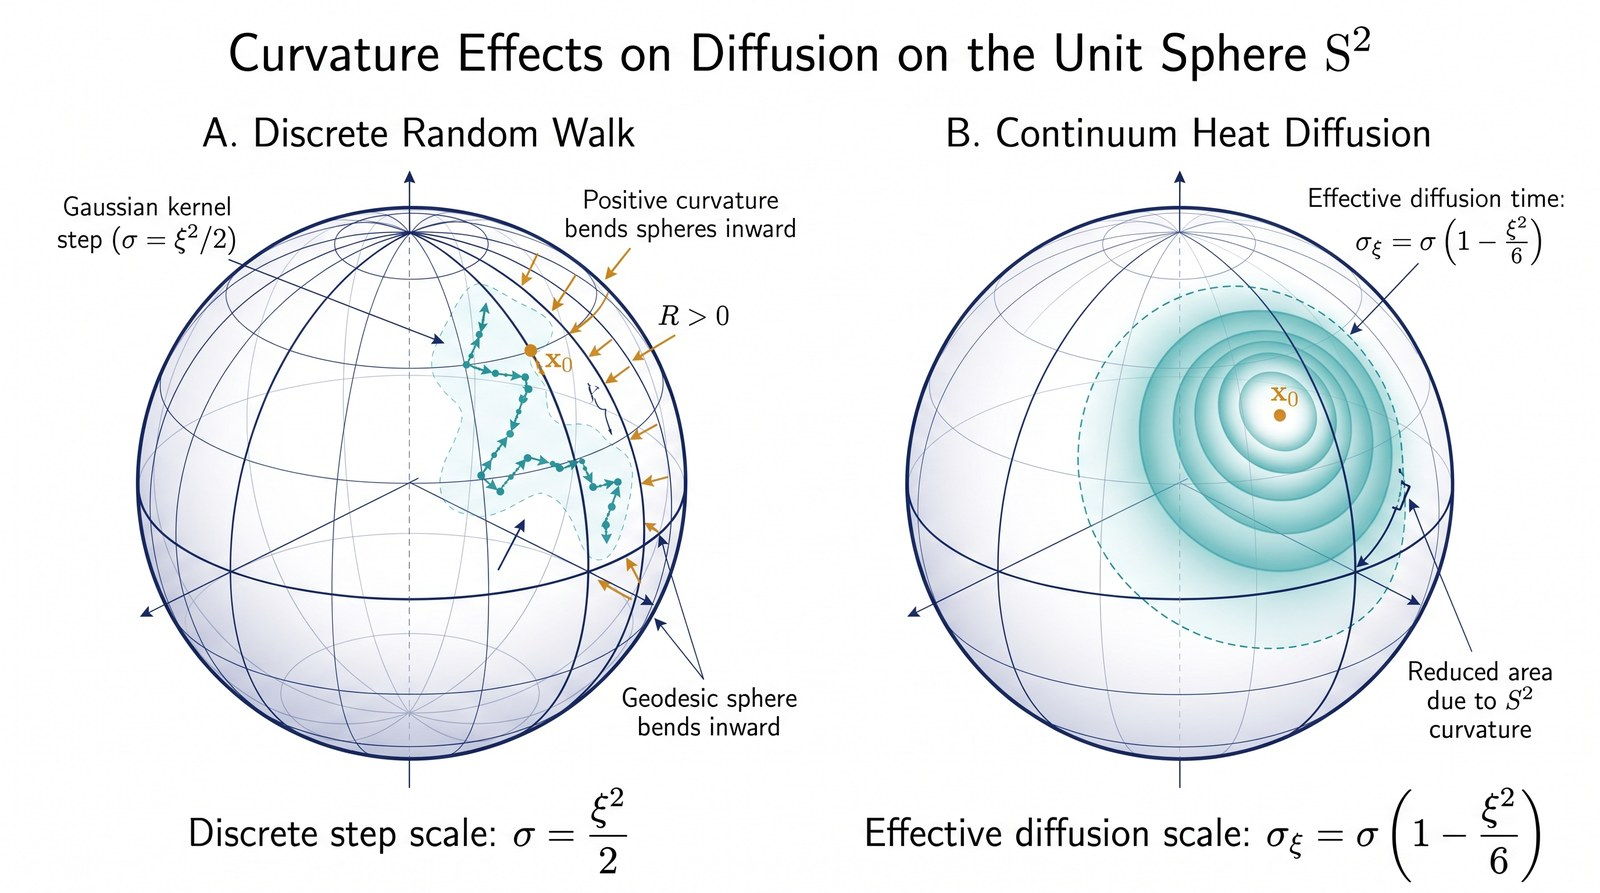
\includegraphics[width=0.86\textwidth]{figures/fig_sphere_rescaling.jpg}
\caption{The round sphere (Propositions~\ref{prop:sphere}, \ref{prop:spheregap}, Corollary~\ref{cor:sphere}). Left: a walk whose step is the Gaussian kernel of scale $\xi$ in the geodesic distance, with the nominal step $\sigma=\xi^2/2$. Right: at the population level it reproduces the heat flow at the rescaled time $\sigma_\xi=\sigma(1-\xi^2/6+O(\xi^4))$, because geodesic circles on the sphere are shorter than in the plane and the second moment of a step is smaller. Schematic, produced as stated in the caption of Figure~\ref{fig:sketch}: the picture omits the remainder $O(\xi^4)$, its labels on curvature paraphrase the shorter circles, the walk shown is a single path and not the population walk, and the small stray marks carry no meaning.}\label{fig:sphere}
\end{figure}

\begin{proposition}[Reduction for the sampled graph]\label{prop:ratereduction}
In the situation of Theorem~\ref{thm:trace}, suppose that the estimate \eqref{eq:eigrate} holds in the second-order form
\begin{equation}\label{eq:eigrate2}
\big|\lambda_k^N-\lambda_k\big|\le C\big(\eta_N+\xi_N^2\,(1+\lambda_k)\big)\lambda_k\qquad\text{for all }k\text{ with }\xi_N\sqrt{\lambda_k}\le c ,
\end{equation}
with some sequence $\eta_N\to0$. Then \eqref{eq:tracerate} holds with $\varepsilon_N/\xi_N+\xi_N/\sqrt t$ replaced by $\eta_N+\xi_N^2/t$.
\end{proposition}

\begin{proof}
Only the estimate of the low modes in the proof of Theorem~\ref{thm:trace} changes:
\[
\sum_{\mathrm{low}}\big|e^{-t\lambda_a^N}-e^{-t\lambda_a}\big|\le C\sum_a\big(\eta_N+\xi^2+\xi^2\lambda_a\big)\,t\lambda_a\,e^{-ct\lambda_a}\le C\Big(\eta_N+\xi^2+\frac{\xi^2}{t}\Big)\Tr e^{(ct/2)\Delta_g},
\]
and $\xi^2\le\xi^2/t$ for $t\le1$.
\end{proof}

The exactly solvable case satisfies \eqref{eq:eigrate2} with $\eta_N=0$, since there $\lambda^N_k=(1-e^{-\sigma\lambda_k})/\sigma$ and $0\le\lambda_k-\lambda_k^N\le\tfrac12\sigma\lambda_k^2$. Open problem~2 is thus reduced to open problem~1: what is missing for the sampled graph is the uniformity in $k$ of the second-order bias, which Theorem~\ref{thm:rate2} provides only for a fixed simple eigenvalue.

\begin{proposition}[The trace in discrete time]\label{prop:discrete}
In the situation of Theorem~\ref{thm:trace}, suppose in addition that the eigenvalues of $S$ are bounded below by $-1+\kappa_0$ for some fixed $\kappa_0>0$ (for example $S\ge0$). Then there are constants $c,C,\kappa>0$ such that almost surely, for all large $N$ and all integers $k\ge2$ with $t=k\,c_h\xi_N^2/2\le1$ and $\xi_N^2\le c\,t$,
\[
\big|\Tr P^k-\Tr e^{t\Delta_g}\big|\le C\Big(\frac{\varepsilon_N}{\xi_N}+\frac{\xi_N}{\sqrt t}+k^{d/2}e^{-\kappa k}\Big)\,t^{-d/2}.
\]
No term is subtracted.
\end{proposition}

\begin{proof}
With the notation of the proof of Theorem~\ref{thm:trace}, $\Tr P^k=\sum_as_a^k$ and $\tau=k$. For a low mode $u=1-s_a=\sigma\lambda_a^N\in[0,\kappa]$ with $\sigma=c_h\xi^2/2$ and $\kappa\le\tfrac12$, and $-u-u^2\le\ln(1-u)\le-u$ gives
\[
0\le e^{-t\lambda_a^N}-s_a^k\le k\,u^2e^{-t\lambda_a^N}=\frac\sigma t\,(t\lambda_a^N)^2e^{-t\lambda_a^N}\le C\,\frac{\xi^2}{t}\,e^{-ct\lambda_a},
\]
where \eqref{eq:eiglow} was used. The sum over the low modes is at most $C(\xi^2/t)\Tr e^{(ct)\Delta_g}$, and $\xi^2/t\le\xi/\sqrt t$. The differences $e^{-t\lambda_a^N}-e^{-t\lambda_a}$ of the low modes and the continuum modes with $a\ge n_{\mathrm{low}}$ are estimated as before. For a high mode $|s_a|\le1-\min(\kappa,\kappa_0)$, hence $|s_a|^k\le(1-\min(\kappa,\kappa_0))^{k-2}s_a^2$, and Lemma~\ref{lem:traces} bounds the sum by $Ce^{-\kappa'k}\xi^{-d}$.
\end{proof}

\begin{proposition}[The bias of the normalised walk at a fixed kernel scale]\label{prop:bias}
Let $\M=\R^d/\mathbb Z^d$ and let $x_1,\dots,x_N$ be independent and uniformly distributed on $\M$. Let $p\colon\M\to[0,\infty)$ be bounded and even with $\int p=1$, and put $M=\sup p$, $p_c=p^{*c}$, $m_1=p(0)$ and $m_c=p_c(0)$ for $c\ge2$. Fix $\rho\in\{p(0),0\}$ (the graph with or without self-loops) and let
\[
g_{ij}=p(x_i-x_j)\ \ (i\ne j),\qquad g_{ii}=\rho,\qquad\tilde P_{ij}=\frac{g_{ij}}N,\qquad\epsilon_i=\sum_j\tilde P_{ij}-1,\qquad P_{ij}=\frac{\tilde P_{ij}\,(1+\epsilon_j)^{-1}}{\sum_l\tilde P_{il}\,(1+\epsilon_l)^{-1}},
\]
with $\Tr P^k:=0$ on the event that some $1+\epsilon_i$ vanishes. For $k\ge1$ let $\mu_1=\rho$, $\mu_k=m_k$ for $k\ge2$,
\[
\Sigma_0=\sum_{l=1}^{k-1}\mu_l\,\mu_{k-l},\qquad\Sigma_c=\sum_{l=1}^{k-1}\int_\M p_l\,p_{k-l}\,p_c\quad(c\ge1),
\]
\[
\beta_k=k\Big[\tfrac12\Sigma_0-2\Sigma_1+3\Sigma_2-2\Sigma_3+\tfrac12\Sigma_4\Big]+k\,\mu_k\big(m_4-3m_3+3m_2-\rho\big).
\]
Then for every $k\ge1$ there are constants $C$ and $N_0$, depending only on $k$ and $M$, such that
\[
\Big|\,\mathbb E\,\Tr P^k-\mu_k-\frac{\beta_k}{N}\Big|\le C\,N^{-3/2}\qquad(N\ge N_0).
\]
\end{proposition}

For $\rho=p(0)$ this is the walk \eqref{eq:W}, \eqref{eq:L} with the estimated normalisation, as in Proposition~\ref{prop:estimated}; for $\rho=0$ it is the same construction with the diagonal of the kernel removed.

\begin{proof}
Throughout, $c_{ij}=g_{ij}-1$, so that $\epsilon_i=\frac1N\sum_jc_{ij}$ and $c_{ii}=\rho-1$. Note $M\ge1$, $0\le g_{ij}\le M$, $|c_{ij}|\le M$, $\int(p-1)=0$, $\int(p-1)^2=m_2-1$, and, $p$ being even, $\int(p(y-v)-1)(p(z-v)-1)\,\dd v=p_2(y-z)-1$. The matrix $\tilde P$ is symmetric.

\emph{Step 1: an exact identity.} Let $\delta=\max_i|\epsilon_i|$ and $E_N=\{\delta\le\frac18\}$. On $E_N$ put $u_i=(1+\epsilon_i)^{-1}$, $r_i=\sum_l\tilde P_{il}u_l>0$ and $\gamma_i=u_i/r_i$. Then $P_{ij}=\tilde P_{ij}u_j/r_i$, and in a closed walk every vertex is once a head and once a tail, so
\begin{equation}\label{eq:bias-identity}
\Tr P^k=\sum_{i_1,\dots,i_k}\ \prod_{a=1}^k\tilde P_{i_ai_{a+1}}\ \prod_{a=1}^k\gamma_{i_a},\qquad i_{k+1}=i_1 .
\end{equation}

\emph{Step 2: expansion of $\gamma_i$.} Fix $i$ and write $e=\epsilon_i$, $b=(\tilde P\epsilon)_i$, $s=(\tilde P\epsilon^2)_i$, $h=(\tilde P|\epsilon|^3)_i$ and $\omega_i=|e|^3+h$. Let
\[
\varphi^1_i=-2e+b,\qquad\varphi^2_i=3e^2-3eb+b^2-s .
\]
We claim that on $E_N$, with an absolute constant $C_0$,
\begin{equation}\label{eq:bias-gamma}
\gamma_i=1+\varphi^1_i+\varphi^2_i+R_i,\qquad|R_i|+|\varphi^1_i|^3+|\varphi^2_i|^{3/2}\le C_0\,\omega_i,\qquad|\gamma_i-1|\le4\delta,\qquad\omega_i\le1 .
\end{equation}
The row sum of $\tilde P$ is $w=1+e\in[\frac78,\frac98]$, so by H\"older's inequality $|b|^3\le w^2h$ and $s^{3/2}\le w^{1/2}h$. Write $u_l=1-\epsilon_l+\epsilon_l^2+\vartheta_l$ with $|\vartheta_l|=|\epsilon_l|^3/(1+\epsilon_l)\le\frac87|\epsilon_l|^3$, and $z=(\tilde P\vartheta)_i$, $|z|\le\frac87h$. Then $r_i=1+\chi$ with $\chi=e-b+s+z$, $|\chi|\le\frac{3}{10}$, and $1/r_i=1-\chi+\chi^2-\chi^3/(1+\chi)$. Multiplying out,
\[
\gamma_i=\big(1-e+e^2+\vartheta_i\big)\Big(1-\chi+\chi^2-\frac{\chi^3}{1+\chi}\Big)=1+\varphi^1_i+\varphi^2_i+R_i,
\]
\[
\begin{aligned}
R_i={}&-z+(s+z)(2e-2b+s+z)-\frac{\chi^3}{1+\chi}+e\Big(s+z-\chi^2+\frac{\chi^3}{1+\chi}\Big)\\
&+e^2\Big(-\chi+\chi^2-\frac{\chi^3}{1+\chi}\Big)+\frac{\vartheta_i}{1+\chi}.
\end{aligned}
\]
Every term of $R_i$ is a product of total order at least three in $(e,b,s^{1/2},z^{1/3})$; by Young's inequality ($|ab|\le\frac13|a|^3+\frac23|b|^{3/2}$) and the bounds on $b$, $s$, $z$ each is at most a constant times $|e|^3+h$. The bounds on $\varphi^1_i$ and $\varphi^2_i$ follow in the same way, $|\gamma_i-1|\le4\delta$ from $\gamma_i\in\big[\frac{1-\delta}{(1+\delta)^2},\frac{1+\delta}{(1-\delta)^2}\big]$, and $\omega_i\le\delta^3(1+w)\le1$.

\emph{Step 3: expansion of the trace.} Let
\[
Q_0=\Tr\tilde P^k,\qquad Q_1=k\sum_i(\tilde P^k)_{ii}\,\varphi^1_i,\qquad Q_2=k\sum_i(\tilde P^k)_{ii}\,\varphi^2_i,\qquad Q_3=\frac k2\sum_{l=1}^{k-1}\sum_{i,j}(\tilde P^l)_{ij}(\tilde P^{k-l})_{ji}\,\varphi^1_i\varphi^1_j ;
\]
these are polynomials in the $g_{ij}$ and are defined everywhere. We claim that on $E_N$
\begin{equation}\label{eq:bias-trace}
\big|\Tr P^k-(Q_0+Q_1+Q_2+Q_3)\big|\le C_1\sum_i(\tilde P^k)_{ii}\,\omega_i\le C_1\,M\,(\tfrac98)^{k-1}\,\frac1N\sum_i\omega_i ,
\end{equation}
with $C_1$ depending only on $k$. Put $\phi_i=\gamma_i-1$ and expand the second product in \eqref{eq:bias-identity}: $\prod_a(1+\phi_{i_a})=1+\sum_a\phi_{i_a}+\sum_{a<b}\phi_{i_a}\phi_{i_b}+E_3$, where $E_3$ is the sum over the subsets $S$ of positions with $|S|\ge3$. Since $|\phi_i|\le\frac12$, each such product is at most $\frac13\sum_{a\in S}|\phi_{i_a}|^3$, so $|E_3|\le\frac{2^k}{3}\sum_{a=1}^k|\phi_{i_a}|^3$. The weights $\prod_a\tilde P_{i_ai_{a+1}}$ are nonnegative, and summing a function of one position, or of two positions at cyclic distance $l$, against them gives $\sum_i(\tilde P^k)_{ii}f(i)$, respectively $\sum_{i,j}(\tilde P^l)_{ij}(\tilde P^{k-l})_{ji}f(i,j)$; there are $k-l$ pairs $a<b$ with $b-a=l$, and for $f(i,j)=f(j,i)$ the expression is symmetric under $l\mapsto k-l$ (rename $i\leftrightarrow j$). Hence
\[
\Tr P^k=Q_0+k\sum_i(\tilde P^k)_{ii}\phi_i+\frac k2\sum_{l=1}^{k-1}\sum_{i,j}(\tilde P^l)_{ij}(\tilde P^{k-l})_{ji}\phi_i\phi_j+E,\qquad|E|\le\frac{2^kk}{3}\sum_i(\tilde P^k)_{ii}|\phi_i|^3 .
\]
Insert $\phi=\varphi^1+\varphi^2+R$ in the linear term and $\phi_i\phi_j=\varphi^1_i\varphi^1_j+\varphi^1_i(\phi_j-\varphi^1_j)+(\phi_i-\varphi^1_i)\phi_j$ in the quadratic one. By \eqref{eq:bias-gamma}, where $\omega_i\le1$ gives $|\phi_i-\varphi^1_i|\le C\omega_i^{2/3}$ and $|\phi_i|\le C\omega_i^{1/3}$, and by Young's inequality, $|\phi_i|^3$, $|R_i|$, $|\varphi^1_i(\phi_j-\varphi^1_j)|$ and $|(\phi_i-\varphi^1_i)\phi_j|$ are bounded by constants times $\omega_i$, respectively $\omega_i+\omega_j$, and $\sum_j(\tilde P^l)_{ij}(\tilde P^{k-l})_{ji}=(\tilde P^k)_{ii}$. This gives the first inequality of \eqref{eq:bias-trace}; the second holds because $\tilde P_{ji}\le M/N$ and the row sums of $\tilde P^{k-1}$ are at most $(1+\delta)^{k-1}$.

\emph{Step 4: the remainder is $O(N^{-3/2})$ in expectation.} Given $x_1$, the variables $Y_l=p(x_1-x_l)-1$, $l\ge2$, are independent, centred, bounded by $M$ and of variance at most $M$, and $\epsilon_1=\frac{\rho-1}N+\frac1N\sum_{l\ge2}Y_l$. From $\mathbb E(\sum_lY_l)^4\le NM^3+3N^2M^2\le4N^2M^3$ we get, for $N\ge M$, $\mathbb E|\epsilon_1|^3\le16\,M^{9/4}N^{-3/2}$, and therefore
\[
\mathbb E\,\omega_i\le\mathbb E|\epsilon_i|^3+\frac MN\sum_l\mathbb E|\epsilon_l|^3\le16\,(1+M)\,M^{9/4}\,N^{-3/2}.
\]
By Bernstein's inequality and the union bound, $\mathbb P(E_N^c)\le2N\exp(-N/(523M))$ for $N\ge16M$. Finally $0\le\Tr P^k\le N$, and $|Q_0|+\dots+|Q_3|\le C_2M^{k+4}$ always, because $|\epsilon_i|\le M$ and $(\tilde P^k)_{ii}\le M^k/N$. With \eqref{eq:bias-trace},
\begin{equation}\label{eq:bias-reduce}
\Big|\,\mathbb E\,\Tr P^k-\mathbb E\,(Q_0+Q_1+Q_2+Q_3)\Big|\le C_3\,N^{-3/2}+\big(N+C_2M^{k+4}\big)\,2N\,e^{-N/(523M)} .
\end{equation}

\emph{Step 5: expectations of polynomial statistics.} Let $V$ be a finite index set with $n$ elements, and let a finite list of edges $(a,b)\in V^2$ be given, each labelled $g$ or $c$. For $\iota\colon V\to\{1,\dots,N\}$ let $G(\iota)$ be the product of the factors $g_{\iota(a)\iota(b)}$, respectively $c_{\iota(a)\iota(b)}$, over the edges. Sorting the maps $\iota$ by the partition $\pi$ of $V$ into their level sets,
\begin{equation}\label{eq:bias-diagram}
N^{-n}\,\mathbb E\sum_\iota G(\iota)=\sum_\pi\frac{N(N-1)\cdots(N-|\pi|+1)}{N^n}\,I_\pi ,
\end{equation}
where $I_\pi=\mathbb E\,G(\iota)$ for any $\iota$ with level sets $\pi$: an integral over $|\pi|$ independent uniform points, with every edge whose two ends lie in the same block replaced by its constant $\rho$ or $\rho-1$. We use: (a) $|I_\pi|\le M^{\#\mathrm{edges}}$; (b) $I_\pi=0$ if some block of $\pi$ is a single index that lies on exactly one edge, and that edge is labelled $c$ and its other end lies in a different block (integrate that point first: $\int(p-1)=0$); (c) the partitions with $|\pi|\le n-2$ contribute $O(N^{-2})$ in total, those with $|\pi|=n-1$ (one pair of indices identified) carry the factor $\frac1N(1+O(\frac1N))$, and the partition into singletons the factor $1-\binom n2\frac1N+O(N^{-2})$. The constants depend only on $n$, the number of edges and $M$.

\emph{Step 6: the nine expectations.} A cycle $i_1,\dots,i_k$ of $g$-edges with distinct indices has $I=\mu_k$. In each statistic below only the listed identifications of one pair survive rule (b); all equalities are up to $O(N^{-2})$.

\smallskip\noindent$Q_0=N^{-k}\sum\prod_ag_{i_ai_{a+1}}$. No identification: $\mu_k(1-\binom k2\frac1N)$. Positions $a<b$ identified, $b-a=l$: two cycles with a common vertex, $I=\mu_l\mu_{k-l}$, where a cycle of length one is a loop and contributes $\mu_1=\rho$; there are $k-l$ such pairs. Hence
\[
\mathbb E\,Q_0=\mu_k+\frac1N\Big[\frac k2\Sigma_0-\frac{k(k-1)}2\mu_k\Big].
\]
\noindent$A=\sum_i(\tilde P^k)_{ii}\epsilon_i=N^{-k-1}\sum\prod_ag_{i_ai_{a+1}}\;c_{i_1v}$. Surviving: $v=i_1$ ($I=(\rho-1)\mu_k$) and, for $k\ge2$, $v=i_r$ with $2\le r\le k$ ($I=\int p_{r-1}p_{k-r+1}p-\mu_k$, since $\int p_{r-1}p_{k-r+1}=m_k$). Hence $\mathbb E\,A=\frac1N[\rho\mu_k+\Sigma_1-k\mu_k]$.

\noindent$B=\sum_i(\tilde P^k)_{ii}(\tilde P\epsilon)_i=N^{-k-2}\sum\prod_ag_{i_ai_{a+1}}\;g_{i_1q}\,c_{qv}$. Surviving: $v=q$ ($(\rho-1)\mu_k$), $v=i_1$ ($\mu_k(m_2-1)$), $v=i_r$, $r\ge2$ (integrating $x_q$ gives $p_2(x_{i_1}-x_{i_r})-1$, so $I=\int p_{r-1}p_{k-r+1}p_2-\mu_k$). Hence $\mathbb E\,B=\frac1N[\rho\mu_k+m_2\mu_k+\Sigma_2-(k+1)\mu_k]$, and
\[
\mathbb E\,Q_1=k\,\mathbb E(-2A+B)=\frac kN\Big[-\rho\mu_k+m_2\mu_k-2\Sigma_1+\Sigma_2+(k-1)\mu_k\Big].
\]
\noindent The four parts of $Q_2$. In each the two $c$-edges end in two indices $v,v'$ of degree one, so only $v=v'$ survives:
\begin{align*}
\textstyle\sum_i(\tilde P^k)_{ii}\epsilon_i^2&:\ c_{i_1v}c_{i_1v'},&I&=\mu_k(m_2-1),\\
\textstyle\sum_i(\tilde P^k)_{ii}\epsilon_i(\tilde P\epsilon)_i&:\ c_{i_1v}\,g_{i_1q}c_{qv'},&I&=\mu_k(m_3-1),\\
\textstyle\sum_i(\tilde P^k)_{ii}(\tilde P\epsilon)_i^2&:\ g_{i_1q}c_{qv}\,g_{i_1q'}c_{q'v'},&I&=\mu_k(m_4-1),\\
\textstyle\sum_i(\tilde P^k)_{ii}(\tilde P\epsilon^2)_i&:\ g_{i_1q}c_{qv}c_{qv'},&I&=\mu_k(m_2-1),
\end{align*}
so that $\mathbb E\,Q_2=\frac{k\mu_k}N\,[3(m_2-1)-3(m_3-1)+(m_4-1)-(m_2-1)]=\frac{k\mu_k}N(2m_2-3m_3+m_4)$.

\noindent The parts of $Q_3$, for fixed $l$: the cycle with the factors attached at the positions $1$ and $l+1$; write $F_l=p_lp_{k-l}$, a function of $x_{i_1}-x_{i_{l+1}}$. Again only $v=v'$ survives:
\begin{align*}
\epsilon_i\epsilon_j&:\ c_{i_1v}c_{i_{l+1}v'},&I&=\textstyle\int F_l\,(p_2-1),\\
\epsilon_i(\tilde P\epsilon)_j\ \text{and}\ (\tilde P\epsilon)_i\epsilon_j&:\ c_{i_1v}\,g_{i_{l+1}q}c_{qv'},&I&=\textstyle\int F_l\,(p_3-1),\\
(\tilde P\epsilon)_i(\tilde P\epsilon)_j&:\ g_{i_1q}c_{qv}\,g_{i_{l+1}q'}c_{q'v'},&I&=\textstyle\int F_l\,(p_4-1).
\end{align*}
With $\varphi^1_i\varphi^1_j=4\epsilon_i\epsilon_j-2\epsilon_i(\tilde P\epsilon)_j-2(\tilde P\epsilon)_i\epsilon_j+(\tilde P\epsilon)_i(\tilde P\epsilon)_j$ and $\int F_l=\mu_k$,
\[
\mathbb E\,Q_3=\frac k{2N}\Big[4\Sigma_2-4\Sigma_3+\Sigma_4-(k-1)\mu_k\Big].
\]
\emph{Step 7: conclusion.} In $\mathbb E(Q_0+Q_1+Q_2+Q_3)$ the terms $k(k-1)\mu_k/N$ cancel ($-\frac12+1-\frac12=0$), and the sum is $\mu_k+\beta_k/N+O(N^{-2})$. With \eqref{eq:bias-reduce} this proves the proposition.
\end{proof}

\begin{remark}[Self-loops and the size of the bias]\label{rem:bias}
(i) With self-loops, $\rho=p(0)=m_1$ and
\[
\beta_k=\frac k2\sum_{l=1}^{k-1}\big[(1-\mathcal P)^4(p_lp_{k-l})\big](0)-k\,m_k\,\Tr\big[\mathcal P(1-\mathcal P)^3\big],
\]
where $\mathcal P$ is the convolution with $p$, $[(1-\mathcal P)^4F](0):=\sum_{c=0}^4(-1)^c\binom4c\int F\,p_c$ with $\int F\,p_0:=F(0)$, and $\Tr[\mathcal P(1-\mathcal P)^3]:=m_1-3m_2+3m_3-m_4$, the trace of that operator when the Fourier series of $p$ is absolutely summable: the bias sees $p_lp_{k-l}$ only through the fourth power of the high-pass filter $1-\mathcal P$. (ii) Without self-loops, for $k\ge3$, $\beta_k^{\rho=0}=\beta_k^{\rho=p(0)}-k\,m_1(m_{k-1}-m_k)$; the difference is the first-order effect of a walk that stays where it is with probability $m_1/N$ in each step, and for the heat kernel with $k\sigma\ll1$ it is close to $\tfrac d2\,m_1m_k$. (iii) The constants $C$, $N_0$ of the proof grow exponentially in $k$ and polynomially in $M$; the proposition says nothing about a regime in which $k$ or $M$ grow with $N$.

(iv) \emph{Numerical check.} For the Gaussian profile on the flat two-torus with $\xi=0.05$ and $N=3000$ (six samples) the mean of $\Tr P^k-m_k$, divided by $m_kM/N$, is $-0.240$, $0.317$, $0.860$, $1.148$, $1.144$ and $1.001$ for $k=1,2,4,8,16,32$, against $-0.250$, $0.313$, $0.893$, $1.200$, $1.186$ and $1.025$ from $\beta_k$; without self-loops ($N=1500$, twelve samples) it is $0.295$, $-0.422$, $0.058$, $0.126$ and $0.038$ for $k=2,4,8,16,32$, against $0.313$, $-0.440$, $0.057$, $0.119$ and $0.039$. In dimensions one and three the agreement is similar. For the subtracted trace at $\xi=0.05$, $N=1500$ (twelve samples) the relative deviation from $T_\sigma$ at $\tau=10,20,40$ is $0.053$, $0.056$ and $0.046$ with self-loops and $-0.002$, $0.007$ and $0.003$ without; the difference of the two traces exceeds the first-order prediction $\frac1N\sum_kw_k(\beta_k^{\rho=p(0)}-\beta_k^{\rho=0})$ by five to eleven percent. These are few samples from one seed and are not evidence for a rate.

(v) \emph{A conjecture.} The proposition and these numbers suggest that for the heat kernel the relative bias of $\Tr P^k$ is a bounded multiple of $M/N$, uniformly in $k$ with $k\sigma\le1$: about $\tfrac d2M/N$ with self-loops and several times smaller without them for $k\ge8$. If this and a corresponding bound for the fluctuations (Remark~\ref{rem:variance}(v)) hold in the joint regime, the rate $\xi^2/t$ holds whenever $N\xi_N^{d+2}\to\infty$, which is much weaker than the condition of Theorem~\ref{thm:jointpoly}. We have no proof: the expansion in $\epsilon$ has a remainder of the order $k^3\delta^3$, the first-order term alone overshoots the difference $\Tr P^k-\Tr\tilde P^k$ in simulations, and the cancellation of the terms of the order $k^2/N$ appears only in the expectation and only when the second order is included.
\end{remark}

\begin{proposition}[The variance of the normalised walk at a fixed kernel scale]\label{prop:variance}
In the setting of Proposition~\ref{prop:bias} let $\Gamma_k=\sum_{l=1}^{k-1}p_l\,p_{k-l}$ (a function on $\M$; $\Gamma_1=0$), let $(1-\mathcal P)^jf=\sum_{c=0}^j(-1)^c\binom jc\,p_c*f$ with $p_0*f=f$, and
\[
H_k=k\,(1-\mathcal P)^4\Gamma_k-2k\,\mu_k\,(1-\mathcal P)^3p,\qquad v_k=\frac12\int_\M H_k^2 .
\]
Then $\int_\M H_k=0$, and for every $k\ge1$ there are $C$, $N_0$ depending only on $k$ and $M$ with
\[
\Big|\operatorname{Var}\Tr P^k-\frac{v_k}{N^2}\Big|\le C\,N^{-5/2}\qquad(N\ge N_0).
\]
With self-loops, $\beta_k=\frac12H_k(0)$.
\end{proposition}

\begin{proof}
Let $Q=Q_0+Q_1+Q_2+Q_3$ be the polynomial statistic of Step~3 of the proof of Proposition~\ref{prop:bias}.

\emph{Step 1: $\|\Tr P^k-Q\|_{L^2}\le CN^{-3/2}$.} On $E_N$, by \eqref{eq:bias-trace} and the Cauchy--Schwarz inequality, $(\Tr P^k-Q)^2\le C\,\frac1N\sum_i\omega_i^2$, and $\omega_i^2\le2\epsilon_i^6+2\big(\sum_l\tilde P_{il}|\epsilon_l|^3\big)^2\le2\epsilon_i^6+\frac{3M}N\sum_l\epsilon_l^6$, the row sum being at most $\frac98$. As in Step~4 there, $\mathbb E(\sum_lY_l)^6\le NM^5+25N^2M^4+15N^3M^3\le41N^3M^5$, hence $\mathbb E\,\epsilon_1^6\le CM^5N^{-3}$ for $N\ge M$. On $E_N^c$ use $|\Tr P^k-Q|\le N+C_2M^{k+4}$ and $\mathbb P(E_N^c)\le2Ne^{-N/(523M)}$. Consequently $|(\operatorname{Var}\Tr P^k)^{1/2}-(\operatorname{Var}Q)^{1/2}|\le CN^{-3/2}$, and it suffices to show $\operatorname{Var}Q=v_k/N^2+O(N^{-3})$.

\emph{Step 2: Hoeffding decomposition.} $Q$ is a symmetric function of $x_1,\dots,x_N$. For $J\subset\{1,\dots,N\}$ let $\eta_J=\sum_{R\subseteq J}(-1)^{|J|-|R|}\,\mathbb E[Q\mid x_R]$; then $Q-\mathbb EQ=\sum_{J\ne\emptyset}\eta_J$ with orthogonal summands, and $\operatorname{Var}Q=\sum_{j\ge1}\binom Nj\,\mathbb E\,\eta_{\{1,\dots,j\}}^2$. Since $Q$ is invariant under a simultaneous translation of all points and the points are uniform, $\mathbb E[Q\mid x_1]$ is constant: $\eta_{\{1\}}=0$.

$Q$ is a finite linear combination of statistics $Z=N^{-n}\sum_\iota G(\iota)$ as in Step~5 there, with $n\le k+4$. If the image of $\iota$ misses some $s\in J$, then $G(\iota)$ does not depend on $x_s$ and its contribution to $\eta_J$ vanishes. There are at most $n^{|J|}N^{n-|J|}$ maps $\iota$ whose image contains $J$, and $|G|\le M^{\#\mathrm{edges}}$; hence $|\eta_J|\le C\,N^{-|J|}$, $\eta_J=0$ for $|J|>k+4$, and $\sum_{j\ge3}\binom Nj\,\mathbb E\,\eta_{\{1,\dots,j\}}^2=O(N^{-3})$.

For $J=\{1,2\}$ and $y=x_1-x_2$: up to $O(N^{-3})$, only the maps contribute that send exactly one position $\alpha$ to the index $1$, exactly one position $\beta\ne\alpha$ to the index $2$, and are injective on the remaining positions, with values outside $\{1,2\}$. For such a map the contribution is $\tilde I_{\alpha\beta}(y)-\int_\M\tilde I_{\alpha\beta}$, where $\tilde I_{\alpha\beta}(y)$ is the integral of the product over the other points; by translation invariance the conditional expectations given $x_1$ or given $x_2$ alone equal $\int\tilde I_{\alpha\beta}$. Therefore
\begin{equation}\label{eq:var-kernel}
N^2\,\eta_{\{1,2\}}=H_Z(y)+O(N^{-1}),\qquad H_Z=\sum_{(\alpha,\beta)}\Big(\tilde I_{\alpha\beta}-\int_\M\tilde I_{\alpha\beta}\Big),
\end{equation}
the sum over the ordered pairs of distinct positions, uniformly in $y$. As in rule (b), $\tilde I_{\alpha\beta}\equiv0$ if an unmarked index lies on exactly one edge and that edge is labelled $c$. With $H=\sum_ZH_Z$, the sum over the statistics $Z$ with their coefficients in $Q$, this gives $\operatorname{Var}Q=\binom N2N^{-4}\int H^2+O(N^{-3})=\frac1{2N^2}\int H^2+O(N^{-3})$.

\emph{Step 3: the marked integrals.} Write $F_s=p_sp_{k-s}$, so that $\Gamma_k=\sum_{s=1}^{k-1}F_s$ and $\int F_s=\mu_k$ for $k\ge2$. In the list the constants $\int\tilde I_{\alpha\beta}$ are already subtracted.

\smallskip\noindent$Q_0$: both marked positions on the cycle, at cyclic distance $s$: $\tilde I=F_s(y)$; summing over the ordered pairs, $H_{Q_0}=k\,\Gamma_k-k(k-1)\mu_k$.

\noindent$A$ (the index $v$ must be marked): with $i_1$: $\mu_k(p(y)-1)$; with $i_r$, $r\ge2$: $(p*F_{r-1})(y)-\mu_k$. There are two orders, so $H_A=2[\mu_k\,p+p*\Gamma_k-k\mu_k]$.

\noindent$B$ ($v$ must be marked): with $q$: $\mu_k(p(y)-1)$; with $i_1$: $\mu_k(p_2(y)-1)$; with $i_r$, $r\ge2$: $(p_2*F_{r-1})(y)-\mu_k$. Hence $H_B=2[\mu_k(p+p_2)+p_2*\Gamma_k-(k+1)\mu_k]$ and
\[
H_{Q_1}=k(-2H_A+H_B)=2k\big[\mu_k(p_2-p)+(p_2-2p)*\Gamma_k+(k-1)\mu_k\big].
\]
\noindent$Q_2$ (both $v$ and $v'$ must be marked; two orders): the four parts give $\mu_k(p_2-1)$, $\mu_k(p_3-1)$, $\mu_k(p_4-1)$ and $\mu_k(p_2-1)$, so
\[
H_{Q_2}=2k\,\mu_k\,(2p_2-3p_3+p_4).
\]
\noindent$Q_3$ (both $v$ and $v'$ must be marked; two orders), for fixed $l$: $p_2*F_l-\mu_k$, $p_3*F_l-\mu_k$ (twice) and $p_4*F_l-\mu_k$, so
\[
H_{Q_3}=k\,(4p_2-4p_3+p_4)*\Gamma_k-k(k-1)\mu_k .
\]
\emph{Step 4: conclusion.} In $H=H_{Q_0}+H_{Q_1}+H_{Q_2}+H_{Q_3}$ the constants cancel ($-1+2-1=0$), the terms with $\Gamma_k$ add up to $k\,(1-4p+6p_2-4p_3+p_4)*\Gamma_k=k(1-\mathcal P)^4\Gamma_k$, and those with $\mu_k$ to $2k\mu_k(-p+3p_2-3p_3+p_4)=-2k\mu_k(1-\mathcal P)^3p$. Hence $H=H_k$. Finally $\int H_k=0$ because $\int(f-p*f)=0$ for every integrable $f$.
\end{proof}

\begin{remark}[The size of the fluctuations]\label{rem:variance}
(i) $H_k$ does not depend on $\rho$ for $k\ge2$: self-loops change the mean of $\Tr P^k$ at the order $1/N$, but its variance only at a higher order. (ii) Formally $\Tr P^k\approx\mu_k+\frac1{N^2}\sum_{a<b}H_k(x_a-x_b)+\frac{\beta_k}N$, and with self-loops the last term is the diagonal $a=b$ of the double sum, $\frac1{2N}H_k(0)$; this is a way to read the two propositions together and not a statement that we prove. (iii) For the heat kernel, with $a_n=e^{-\sigma\lambda_n}$, the Fourier coefficients are $\hat H_k(n)=k(1-a_n)^4\hat\Gamma_k(n)-2k\mu_ka_n(1-a_n)^3$ with $\hat\Gamma_k(n)=\sum_l\sum_{n_1}a_{n_1}^l\,a_{n-n_1}^{k-l}$, and $v_k=\frac12\sum_{n\ne0}\hat H_k(n)^2$.

(iv) \emph{Numerical check.} On the flat two-torus with $\xi=0.15$ and $N=800$ (600 samples, with self-loops), $N$ times the standard deviation of $\Tr P^k$ is $3.69$, $2.36$, $2.98$, $1.54$ for $k=1,2,4,8$, with a statistical error of three percent, against $\sqrt{v_k}=3.49$, $2.33$, $2.93$, $1.48$. For $\xi=0.08$ and $N=1000$ (200 samples), where $M/N$ is about three times larger, the observed values $27.6$, $16.9$, $21.8$, $15.8$ exceed $\sqrt{v_k}=23.4$, $15.9$, $19.2$, $13.8$ by $7$ to $18$ percent, with a statistical error of five percent: the terms of higher order are not small there.

(v) For the heat kernel and $k\sigma\ll1$ one finds numerically $v_k\approx c_k\,M\,m_k^2$ with $c_k$ of order one (between $0.04$ and $0.8$ for $k\le16$ in dimension two), so that the relative fluctuation of $\Tr P^k$ is of the order $\sqrt M/N$, smaller than the relative bias of the order $M/N$ of Remark~\ref{rem:bias}(v). In this form the conjecture of that remark reads $\Tr P^k/m_k=1+b_kM/N+O_{\mathbb P}(\sqrt M/N)$ with bounded $b_k$, uniformly in $k$ with $k\sigma\le1$. It is not proven: the constants of the two propositions are not uniform in $k$ and $M$.
\end{remark}

\paragraph{The kernel of the sampled walk} The remaining statements of this subsection concern the walk itself and not only its trace. For $t>0$ let $\gamma_t(v)=(2\pi t)^{-d/2}e^{-|v|^2/2t}$ on $\R^d$ and $p^{(t)}(w)=\sum_{n\in\mathbb Z^d}\gamma_t(w+n)$ on $\M=\R^d/\mathbb Z^d$, the heat kernel of $\M$ at the time $t/2$. Thus $p=p^{(\xi^2)}$, $p_m=p^{*m}=p^{(m\xi^2)}$, $M=p(0)$, $m_m=p_m(0)$, and $(\mathcal Pf)(x)=\int_\M p(x-y)f(y)\,\dd y$. The points $x_1,\dots,x_N$ are independent and uniform on $\M$, $\tilde P_{bj}=p(x_b-x_j)/N$ (self-loops included), $\epsilon_b=\sum_j\tilde P_{bj}-1$, $\delta=\max_b|\epsilon_b|$, $u_j=(1+\epsilon_j)^{-1}$, $r_b=\sum_j\tilde P_{bj}u_j$ and $P_{bj}=\tilde P_{bj}u_j/r_b$. For $1\le i\le N$ and $m\ge1$,
\[
h^{(i)}_m(b)=\sum_jP_{bj}\,p_m(x_j-x_i)-p_{m+1}(x_b-x_i).
\]

\begin{lemma}[Facts on the periodised Gaussian]\label{lem:pgauss}
There is a constant $C_d\ge1$ such that for all $t>0$, $0<a\le\min(t,1)$ and $u,z\in\M$:
\begin{enumerate}[label=\textup{(P\arabic*)}]
\item $p^{(a)}\le(t/a)^{d/2}\,p^{(t)}$ pointwise;
\item $\sup p^{(t)}=p^{(t)}(0)$ is non-increasing in $t$; $p^{(t)}(0)\le C_dt^{-d/2}$ for $t\le2$, $p^{(t)}(0)\le C_d$ for $t\ge2$, and $p^{(t)}\ge\frac12$ for $t\ge t_d$, where $t_d\ge1$ depends only on $d$;
\item $|\nabla p^{(t)}|\le2^{d/2}\,t^{-1/2}\,p^{(2t)}$ pointwise;
\item $p^{(a)}(u)\,p^{(t)}(z-u)\le C_d\,(2\pi a)^{-d/2}\,p^{(3t)}(z)$;
\item $\big(p^{(2t)}(0)\,p^{(3t)}(z)\big)^{1/2}\le C_d\,p^{(6t)}(z)$.
\end{enumerate}
\end{lemma}

\begin{proof}
(P1): $\gamma_a\le(t/a)^{d/2}\gamma_t$ for $a\le t$. (P2): $p^{(t)}(w)=\sum_{k\in\mathbb Z^d}e^{-2\pi^2|k|^2t}e^{2\pi ik\cdot w}$ has positive coefficients that decrease in $t$; $p^{(t)}(0)=(2\pi t)^{-d/2}\big(\sum_{j\in\mathbb Z}e^{-j^2/2t}\big)^d\le(2\pi t)^{-d/2}\big(1+2\sum_{j\ge1}e^{-j^2/4}\big)^d$ for $t\le2$; and $|p^{(t)}-1|\le\sum_{k\ne0}e^{-2\pi^2|k|^2t}=\big(1+2\sum_{j\ge1}e^{-2\pi^2j^2t}\big)^d-1\le\frac12$ for $t\ge t_d$. (P3): $\nabla\gamma_t(v)=-(v/t)\gamma_t(v)$ and $re^{-r^2/2}\le e^{-r^2/4}$ for $r\ge0$ give $|\nabla\gamma_t|\le t^{-1/2}2^{d/2}\gamma_{2t}$; sum over the lattice. (P4): for $v,v'\in\R^d$, $\frac{|v|^2}{2a}+\frac{|v'|^2}{2t}\ge\frac{|v|^2}{4a}+\frac{|v+v'|^2}{2(t+2a)}$, because $\frac{|v|^2}{4a}+\frac{|v'|^2}{2t}\ge\frac{|v+v'|^2}{4a+2t}$ by the Cauchy--Schwarz inequality. With $v=u+n$, $v'=z-u+n'$ and $n''=n+n'$,
\[
\begin{aligned}
p^{(a)}(u)\,p^{(t)}(z-u)&\le(2\pi a)^{-d/2}(2\pi t)^{-d/2}\sum_ne^{-|u+n|^2/4a}\ \sum_{n''}e^{-|z+n''|^2/2(t+2a)}\\
&\le C\,(2\pi a)^{-d/2}\Big(\frac{t+2a}{t}\Big)^{d/2}p^{(t+2a)}(z),
\end{aligned}
\]
since $\sum_ne^{-|u+n|^2/4a}\le(2+2\sum_{j\ge1}e^{-j^2/4})^d$ for $a\le1$; now use $t+2a\le3t$ and (P1). (P5): for $t\le1$, $\big(p^{(3t)}(z)\big)^{1/2}\le\sum_n\gamma_{3t}(z+n)^{1/2}=(24\pi t)^{d/4}p^{(6t)}(z)$ and $p^{(2t)}(0)\le C_d(2t)^{-d/2}$; for $1\le t\le t_d$ the same computation applies with $p^{(2t)}(0)\le C_d$ and $(24\pi t)^{d/4}\le C_d$; for $t\ge t_d$ the left-hand side is bounded and $p^{(6t)}\ge\frac12$, by (P2).
\end{proof}

\begin{lemma}[Consistency of the normalised walk]\label{lem:consistency}
Let $d\ge1$, $0<\xi\le1$, $N\ge3$, $M\log N\le N$, $\delta'=\sqrt{M\log N/N}$ and $6\delta'\le\frac18$. There is a constant $C$ depending only on $d$ such that, with probability at least $1-7N^{-3}$, the following hold for all $b,i\in\{1,\dots,N\}$ and all integers $1\le m\le\delta'^{-2}$:
\begin{enumerate}[label=\textup{(\roman*)}]
\item $\delta\le6\delta'$;
\item $\big|h^{(i)}_m(b)\big|\le C\,\delta'\,m^{-1/2}\,p_{6m}(x_b-x_i)$;
\item $\frac1N\sum_bp_{6m}(x_b-x_i)\le1+9\delta'$.
\end{enumerate}
In particular $\max_b|h^{(i)}_m(b)|\le C\delta'm^{-1/2}m_{6m}$ and $\frac1N\sum_b|h^{(i)}_m(b)|\le2C\delta'm^{-1/2}$.
\end{lemma}

\begin{proof}
We use Bernstein's inequality in the following form: if $X_1,\dots,X_n$ are independent and centred, $|X_j|\le B$ and $\mathbb EX_j^2\le v$, then for every $L>0$, with probability at least $1-2e^{-L}$, $|\sum_jX_j|\le\sqrt{2nvL}+\frac23BL$. Throughout $L=6\log N$, and $C$ denotes constants that depend only on $d$.

\emph{\textup{(i)}} is Step~1 of the proof of Theorem~\ref{thm:jointpoly} and fails with probability at most $2N^{-3}$.

\emph{\textup{(iii)}.} Fix $i$ and $m$. Given $x_i$, the variables $p_{6m}(x_b-x_i)-1$, $b\ne i$, are independent and centred, bounded by $\max(m_{6m},1)\le M$ and of variance at most $\int p_{6m}^2=m_{12m}\le M$, by (P2). With probability at least $1-2N^{-6}$ their sum is at most $\sqrt{12MN\log N}+4M\log N$ in absolute value, that is, at most $N(\sqrt{12}\,\delta'+4\delta'^2)$; the term $b=i$ contributes $m_{6m}/N\le\delta'^2$. Since $\delta'\le1$ this gives (iii), and the union over $i$ and $m\le\delta'^{-2}\le N$ costs at most $2N^{-4}$.

\emph{\textup{(ii)}.} Fix $b$, $i$, $m$, put $s=m\xi^2$, $z=x_b-x_i$, $g=p_m(\cdot-x_i)$ and $c_b=(\mathcal Pg)(x_b)=p_{m+1}(z)$. Since $\sum_jP_{bj}=1$,
\begin{equation}\label{eq:cons-split}
h^{(i)}_m(b)=\frac1{r_b}\,(S_1+S_2),\qquad S_1=\sum_j\tilde P_{bj}\big(g(x_j)-c_b\big),\qquad S_2=\sum_j\tilde P_{bj}(u_j-1)\big(g(x_j)-c_b\big).
\end{equation}
On the event (i), $\delta\le\frac18$, hence $1/r_b\le\frac{10}7$ and $|u_j-1|\le\frac87\delta$, so that
\[
\big|h^{(i)}_m(b)\big|\le\tfrac{10}7\big(|S_1|+\tfrac87\,\delta\,A\big),\qquad A=\frac1N\sum_jp(x_b-x_j)\,\big|g(x_j)-c_b\big| .
\]
For $j\notin\{b,i\}$ let $Y_j=p(x_b-x_j)\,(g(x_j)-c_b)$. Given $x_b$ and $x_i$ the $Y_j$ are independent and identically distributed, and $\mathbb EY_j=\int p(x_b-y)p_m(y-x_i)\,\dd y-c_b=0$.

\emph{A bound for $Y_j$.} By (P4) with $a=\xi^2$, $t=s$ and $(2\pi\xi^2)^{-d/2}\le M$, $p(x_b-y)\,p_m(y-x_i)\le CM\,p^{(3s)}(z)$ for all $y$, and $c_b=p^{(s+\xi^2)}(z)\le3^{d/2}p^{(3s)}(z)$ by (P1). Hence
\begin{equation}\label{eq:cons-B}
|Y_j|\le B:=C\,M\,p^{(3s)}(z).
\end{equation}
\emph{The variance.} For a function $f$ on $\M$, $\int_\M p(x_b-y)f(y)\,\dd y=\mathbb E\,f(x_b+\xi Z)$ with a standard Gaussian vector $Z$ in $\R^d$ ($f$ extended periodically). Hence $c_b=\mathbb E\,g(x_b+\xi Z)$ and, by the Gaussian Poincar\'e inequality, (P3), (P2) and $\mathcal Pp^{(2s)}=p^{(2s+\xi^2)}\le(\frac32)^{d/2}p^{(3s)}$,
\begin{align}
\mathbb EY_j^2&\le M\int p(x_b-y)\,(g(y)-c_b)^2\,\dd y=M\operatorname{Var}g(x_b+\xi Z)\le M\,\xi^2\,\big(\mathcal P|\nabla p_m|^2\big)(z)\notag\\
&\le M\,\xi^2\,\frac{2^d}{s}\,p^{(2s)}(0)\,\big(\mathcal Pp^{(2s)}\big)(z)\le v:=\frac{C\,M}{m}\,p^{(2s)}(0)\,p^{(3s)}(z),\label{eq:cons-v}
\end{align}
and $\mathbb E|Y_j|\le(v/M)^{1/2}$ by the Cauchy--Schwarz inequality.

\emph{Bernstein.} With probability at least $1-2N^{-6}$, by \eqref{eq:cons-B}, \eqref{eq:cons-v}, (P1) and (P5),
\[
\begin{aligned}
\Big|\frac1N\sum_{j\notin\{b,i\}}Y_j\Big|&\le\sqrt{\frac{12\,v\log N}{N}}+\frac{4B\log N}{N}\le C\,\delta'\,m^{-1/2}\big(p^{(2s)}(0)\,p^{(3s)}(z)\big)^{1/2}+C\,\delta'^2\,p^{(3s)}(z)\\
&\le C\,\delta'\,m^{-1/2}\,p^{(6s)}(z),
\end{aligned}
\]
where the last step uses $\delta'\le m^{-1/2}$. The same bound holds, with the same probability, for $\frac1N\sum_{j\notin\{b,i\}}(|Y_j|-\mathbb E|Y_j|)$, because $\big||Y_j|-\mathbb E|Y_j|\big|\le B$ and $\operatorname{Var}|Y_j|\le v$.

\emph{The two exceptional terms.} The term $j=b$ of $S_1$ and of $A$ is at most $\frac MN\,(p_m(z)+p_{m+1}(z))\le C\,\frac MN\,p^{(3s)}(z)$ in absolute value, by (P1). For $b\ne i$ the term $j=i$ is at most $\frac1N\,(p(z)\,p_m(0)+M\,c_b)\le C\,\frac MN\,p^{(3s)}(z)$, by (P4) with $u=z$. Since $M/N\le\delta'^2\le\delta'm^{-1/2}$ and $p^{(3s)}\le2^{d/2}p^{(6s)}$, both are at most $C\delta'm^{-1/2}p^{(6s)}(z)$.

\emph{Conclusion.} On the intersection of these events, $|S_1|\le C\delta'm^{-1/2}p^{(6s)}(z)$ and
\[
\begin{aligned}
A&\le\mathbb E|Y_j|+C\,\delta'm^{-1/2}p^{(6s)}(z)\le C\,m^{-1/2}\big(p^{(2s)}(0)p^{(3s)}(z)\big)^{1/2}+C\,\delta'm^{-1/2}p^{(6s)}(z)\\
&\le C\,m^{-1/2}\,p^{(6s)}(z),
\end{aligned}
\]
again by (P5). With $\delta\le6\delta'$ and $p^{(6s)}=p_{6m}$ this is (ii). There are at most $N^2\delta'^{-2}\le N^3$ triples $(b,i,m)$ and two events for each, so (ii) fails with probability at most $4N^{-3}$; together with (i) and (iii) the total is at most $7N^{-3}$. The last two statements follow from $p_{6m}\le m_{6m}$ and from (iii) with $9\delta'\le1$.
\end{proof}

\begin{theorem}[The kernel of the sampled walk, uniformly in the number of steps]\label{thm:kernel}
In the situation of Lemma~\ref{lem:consistency} let $m_s=p^{(s\xi^2)}(0)$ for real $s>0$, let
\[
D_k=\max_{a,i}\big|N(P^k)_{ai}-p_k(x_a-x_i)\big|,
\]
and let $C_1=24+3\cdot2^{d+3}C$ with the constant $C$ of the lemma. On the event of the lemma, for all integers $k$ with $1\le k\le(C_1\delta')^{-2}$,
\[
D_k\le C_1\,\delta'\,\sqrt k\;m_k,\qquad\text{in particular}\qquad\big|\Tr P^k-m_k\big|\le C_1\,\delta'\,\sqrt k\;m_k .
\]
\end{theorem}

\begin{proof}
By (P2) and (P1), $s\mapsto m_s$ is non-increasing and $m_s\le2^{d/2}m_{2s}$.

\emph{Step 1: telescoping.} Let $R$ be the restriction of functions on $\M$ to the points, and write $(Pg)(b)=\sum_jP_{bj}\,g(x_j)$. For every $g$ and $k\ge1$,
\[
P^kRg-R\mathcal P^kg=\sum_{l=0}^{k-1}P^l\,(PR-R\mathcal P)\,\mathcal P^{k-1-l}g .
\]
For $g_i=p(\cdot-x_i)$ one has $\mathcal P^ng_i=p_{n+1}(\cdot-x_i)$ and $(PR-R\mathcal P)\,p_m(\cdot-x_i)=h^{(i)}_m$. With $m=k-l$,
\begin{equation}\label{eq:kernel-telescope}
(P^kRg_i)(a)=p_{k+1}(x_a-x_i)+\sum_{m=1}^k\big(P^{k-m}h^{(i)}_m\big)(a).
\end{equation}
\emph{Step 2: the last step of the walk.} As in Step~2 of the proof of Theorem~\ref{thm:jointpoly}, $NP_{bi}=p(x_b-x_i)(1+\theta_{bi})$ with $|\theta_{bi}|\le4\delta$ for $\delta\le\frac18$. Since $N(P^{k+1})_{ai}=\sum_b(P^k)_{ab}\,NP_{bi}$ and the entries of $P^k$ are nonnegative, $|N(P^{k+1})_{ai}-(P^kRg_i)(a)|\le4\delta\,(P^kRg_i)(a)$. With \eqref{eq:kernel-telescope} and $p_{k+1}\le m_{k+1}$,
\begin{equation}\label{eq:kernel-rec}
D_{k+1}\le4\delta\,m_{k+1}+(1+4\delta)\,S_k,\qquad S_k=\max_{a,i}\Big|\sum_{m=1}^k\big(P^{k-m}h^{(i)}_m\big)(a)\Big| .
\end{equation}
\emph{Step 3: two bounds for one term.} $P^l$ is row-stochastic, hence $|(P^lh)(a)|\le\max_b|h(b)|$; and for $l\ge1$, $|(P^lh)(a)|\le\max_bN(P^l)_{ab}\cdot\frac1N\sum_b|h(b)|\le(m_l+D_l)\,\frac1N\sum_b|h(b)|$. By the lemma, $\max_b|h^{(i)}_m(b)|\le C\delta'm^{-1/2}m_{6m}$ and $\frac1N\sum_b|h^{(i)}_m(b)|\le2C\delta'm^{-1/2}$.

\emph{Step 4: induction.} We show $D_k\le C_1\delta'\sqrt k\,m_k$ for $1\le k\le(C_1\delta')^{-2}$. For $k=1$, $|NP_{ai}-p(x_a-x_i)|\le4\delta M\le24\,\delta'm_1$. Let the claim hold up to $k$, with $k+1\le(C_1\delta')^{-2}$; then $D_l\le m_l$ for $l\le k$, and all $m\le k$ are in the range of the lemma. In $S_k$ use the first bound of Step~3 for $m>k/2$ and the second for $m\le k/2$. For $m>k/2$, $6m\ge k+1$ and $m_{6m}\le m_{k+1}$. For $m\le k/2$, $k-m\ge k/2\ge(k+1)/4$, so $m_{k-m}+D_{k-m}\le2m_{(k+1)/4}\le2^{d+1}m_{k+1}$. Hence
\[
S_k\le C\,\delta'\,m_{k+1}\Big[\sum_{k/2<m\le k}m^{-1/2}+2^{d+2}\sum_{m\le k/2}m^{-1/2}\Big]\le2^{d+3}C\,\delta'\,\sqrt k\;m_{k+1},
\]
and by \eqref{eq:kernel-rec}, with $\delta\le6\delta'\le\frac18$, $D_{k+1}\le\big(24+\tfrac32\cdot2^{d+3}C\big)\delta'\sqrt{k+1}\,m_{k+1}\le C_1\delta'\sqrt{k+1}\,m_{k+1}$. Finally $\Tr P^k-m_k=\frac1N\sum_i\big(N(P^k)_{ii}-p_k(0)\big)$.
\end{proof}

\begin{corollary}[The joint regime, almost surely]\label{cor:kernel-trace}
Let $\M=\R^d/\mathbb Z^d$, $d\ge1$, with the uniform density and the periodised Gaussian kernel, and let $\xi_N\to0$ and $N\xi_N^{d+2}/\log N\to\infty$. Then almost surely, for all large $N$, all $t\in[\xi_N^2,1]$ and all integers $1\le k\le20\,\xi_N^{-2}$, with $\sigma=\xi_N^2/2$, $\tau=2t/\xi_N^2$ and $\delta'=\sqrt{M\log N/N}$,
\[
\Big|\frac{\Tr P^k}{\Tr e^{k\sigma\Delta}}-1\Big|\le C_1\,\delta'\sqrt k,\qquad\Big|\frac{\Tr e^{-t\Lc}-Ne^{-\tau}}{T_\sigma(t)}-1\Big|\le C_1\,\delta'\sqrt{8\tau+2\log N+2}+\frac{4M}{N^2},
\]
and both right-hand sides are at most $C\big(\log N\,(1+\xi_N^2\log N)/N\xi_N^{d+2}\big)^{1/2}$, which tends to zero. If moreover $N\xi_N^{d+6}/\log N\to\infty$, they are $o(\xi_N^2)$, and almost surely
\[
\frac{\Tr e^{-t_N\Lc}-Ne^{-\tau}}{\Tr e^{t_N\Delta}}=1+\frac{d(d+2)}{8\tau}+O(\tau^{-2})+O(\xi_N^2)+o(\xi_N^2)
\]
for every sequence $t_N\in[\xi_N^2,1]$: the rate $\xi^2/t$ of open problem~2 holds with the sharp coefficient, almost surely, in this regime.
\end{corollary}

\begin{proof}
The probabilities $7N^{-3}$ are summable, so almost surely the event of Lemma~\ref{lem:consistency} holds for all large $N$. Let $J=\lceil8\tau\rceil+\lceil2\log N\rceil$; then $J\le16\,\xi_N^{-2}+2\log N+2$ and $\delta'^2J\le CM\log N\,(\xi_N^{-2}+\log N)/N\to0$; for the second summand note that the assumption gives $M\le C\xi_N^{-d}\le C(N/\log N)^{d/(d+2)}$ for large $N$, hence $M(\log N)^2/N\le C(\log N)^{2-d/(d+2)}N^{-2/(d+2)}\to0$. Consequently $J$ and $20\,\xi_N^{-2}$ are at most $(C_1\delta')^{-2}$ for large $N$, and the conditions $M\log N\le N$ and $6\delta'\le\frac18$ hold. The first statement is the theorem with $m_k=\Tr e^{k\sigma\Delta}$. For the second, $\Tr e^{-t\Lc}-Ne^{-\tau}=\sum_{j\ge1}w_j\Tr P^j$ by Theorem~\ref{thm:poisson} and $T_\sigma(t)=\sum_{j\ge1}w_jm_j$ by Theorem~\ref{thm:rate}(i), with $w_j=e^{-\tau}\tau^j/j!$. For $j\le J$ use the theorem and $\sqrt j\le\sqrt J$. For $j>J$, where $j\ge2$: $\Tr P^j\le\Tr P^2$ by Proposition~\ref{prop:moments}(ii), $\Tr P^2\le m_2+D_2\le2m_2\le2M$ by the theorem, $m_j\le M$, and $\sum_{j>J}w_j\le N^{-2}$ as in Step~4 of the proof of Theorem~\ref{thm:jointpoly}. Finally $T_\sigma(t)\ge\sum_{j\ge1}w_j=1-e^{-\tau}\ge\frac34$, because $m_j\ge1$ and $\tau\ge2$. If $N\xi_N^{d+6}/\log N\to\infty$, then $\delta'^2J=o(\xi_N^4)$: for $\log N\le\xi_N^{-2}$ it is at most $CM\log N\,\xi_N^{-2}/N$, and otherwise at most $CM(\log N)^2/N$ with $\xi_N^2>1/\log N$ and $M\le C\xi_N^{-d}\le C(\log N)^{d/2}$. The last statement follows from the uniform form of \eqref{eq:rateexact} in Step~5 of the proof of Theorem~\ref{thm:jointpoly}.
\end{proof}

\begin{corollary}[The corrected estimator on the sampled graph]\label{cor:kernel-corrected}
In the situation of Corollary~\ref{cor:kernel-trace} let $T^N(t)=\Tr e^{-t\Lc}-Ne^{-\tau}$. Almost surely, for all large $N$ and all $t\in[\xi_N^2,1]$,
\[
\Big|\Big(T^N-\frac{\sigma t}2\,(T^N)''\Big)(t)-\Big(T_\sigma-\frac{\sigma t}2\,T_\sigma''\Big)(t)\Big|\le(1+3\tau)\,C_1\,\delta'\sqrt{8\tau+2\log N+4}\;T_\sigma(t)+(3+6\tau)\frac M{N^2},
\]
where the derivatives are taken with respect to $t$. Consequently the relative deviation of the corrected estimator of the sampled graph from $\Tr e^{t\Delta}$ is $O(\tau^{-2})+O\big(\tau\,\delta'\sqrt{\tau+\log N}\big)$.
\end{corollary}

\begin{proof}
Let $a_j=\Tr P^j$ and $e_j=a_j-m_j$ for $j\ge1$, and $w_j=e^{-\tau}\tau^j/j!$ for $j\ge0$, $w_{-1}=0$. Then $T^N-T_\sigma=\sum_{j\ge1}w_je_j$, a series that may be differentiated term by term because $|e_j|\le N+M$, and $\frac{\dd^2}{\dd\tau^2}w_j=w_{j-2}-2w_{j-1}+w_j$. Hence
\[
\frac{\dd^2}{\dd\tau^2}\big(T^N-T_\sigma\big)=\sum_{i\ge0}w_i\,e_{i+2}-2\sum_{i\ge0}w_i\,e_{i+1}+\sum_{i\ge1}w_i\,e_i .
\]
Let $J$ be as in the proof of Corollary~\ref{cor:kernel-trace}; for large $N$, $J+2\le(C_1\delta')^{-2}$. For the indices up to $J+2$, $|e_j|\le C_1\delta'\sqrt{J+2}\,m_j$ by Theorem~\ref{thm:kernel}, and $\sum_{i\ge0}w_im_{i+2}\le\sum_{i\ge0}w_im_{i+1}\le e^{-\tau}M+T_\sigma\le\frac32T_\sigma$, because $m_j$ is non-increasing, $T_\sigma\ge w_1m_1=\tau e^{-\tau}M$ and $\tau\ge2$. The terms with $i\le J$ therefore contribute at most $\frac{11}2C_1\delta'\sqrt{J+2}\,T_\sigma$. For $i>J$ all indices are at least two, $|e_j|\le a_j+m_j\le3M$ as in the proof of Corollary~\ref{cor:kernel-trace}, and $\sum_{i>J}w_i\le N^{-2}$, which gives at most $12MN^{-2}$. Since $t=\sigma\tau$, $\frac{\sigma t}2\frac{\dd^2}{\dd t^2}=\frac\tau2\frac{\dd^2}{\dd\tau^2}$; together with $|T^N-T_\sigma|\le C_1\delta'\sqrt J\,T_\sigma+3MN^{-2}$ from the same proof this is the first statement, with $J+2\le8\tau+2\log N+4$. The second follows from Theorem~\ref{thm:corrected} and $T_\sigma\le C\,\Theta$.
\end{proof}

\begin{corollary}[The graph without self-loops]\label{cor:kernel-noloops}
Let $P$ be built as in Lemma~\ref{lem:consistency}, but with the diagonal of the kernel removed, that is, with $\tilde P_{bb}=0$ (the case $\rho=0$ of Proposition~\ref{prop:bias}). Then Lemma~\ref{lem:consistency} holds without change, $D_1=m_1$, and on the event of the lemma, with $C_1'=C_1+3\cdot2^{d/2}$,
\[
D_k\le C_1'\,\delta'\,\sqrt k\;m_k\qquad\text{for all integers }2\le k\le(C_1'\delta')^{-2}.
\]
In the situation of Corollary~\ref{cor:kernel-trace}, almost surely for all large $N$ and all $t\in[\xi_N^2,1]$,
\[
\Big|\Tr e^{-t\Lc}-Ne^{-\tau}-\big(T_\sigma(t)-\tau e^{-\tau}M\big)\Big|\le\Big(C_1'\,\delta'\sqrt{8\tau+2\log N+2}+\frac{4M}{N^2}\Big)\,T_\sigma(t),
\]
and $\tau e^{-\tau}M\le C\,\tau^{1+d/2}e^{-\tau}\,\Tr e^{t\Delta}$: the statements of Corollary~\ref{cor:kernel-trace} on the rate hold for the graph without self-loops as well.
\end{corollary}

\begin{proof}
\emph{The lemma.} In its proof the term $j=b$ of $S_1$ and of $A$ is absent, and in (i) the term $l=i$ is replaced by $-1/N$, since now $\epsilon_i=\frac1N\sum_{l\ne i}(p(x_i-x_l)-1)-\frac1N$; nothing else changes.

\emph{The recursion.} Now $NP_{bi}=p(x_b-x_i)(1+\theta_{bi})$ for $b\ne i$ and $NP_{ii}=0$, hence
\[
N(P^{k+1})_{ai}=\sum_b(P^k)_{ab}\,g_i(x_b)(1+\theta_{bi})-M\,(1+\theta_{ii})\,(P^k)_{ai},
\]
with $\theta_{ii}$ defined by the same formula as for $b\ne i$, $|\theta_{ii}|\le4\delta$. Since $N(P^k)_{ai}\le m_k+D_k$, \eqref{eq:kernel-rec} becomes
\[
D_{k+1}\le4\delta\,m_{k+1}+(1+4\delta)\,S_k+(1+4\delta)\,\frac MN\,(m_k+D_k).
\]
For $k=1$ the diagonal entry gives $D_1=m_1$, the other entries being at most $4\delta M$ apart. In the induction of Step~4 the hypothesis is used only in the form $D_l\le m_l$, which holds for $l=1$; the additional term is at most $3\frac MNm_k\le3\cdot2^{d/2}\delta'^2m_{k+1}$, because $M/N\le\delta'^2$ and $m_k\le2^{d/2}m_{2k}\le2^{d/2}m_{k+1}$. For $k=1$ one has $S_1\le C\delta'm_6\le C\delta'm_2$, so that $D_2\le C_1'\delta'\sqrt2\,m_2$, and the induction proceeds as before with $C_1'$ in place of $C_1$.

\emph{The trace.} Here $\Tr P=0$, so that $\Tr e^{-t\Lc}-Ne^{-\tau}=\sum_{j\ge2}w_j\Tr P^j$, to be compared with $\sum_{j\ge2}w_jm_j=T_\sigma(t)-\tau e^{-\tau}M$. The terms with $2\le j\le J$ and with $j>J$ are estimated as in the proof of Corollary~\ref{cor:kernel-trace}. Finally $M\le C\sigma^{-d/2}$ and $\Tr e^{t\Delta}\ge(4\pi t)^{-d/2}$ give $M\le C\tau^{d/2}\Tr e^{t\Delta}$.
\end{proof}

\begin{proposition}[Reduction of the trace to a polynomial statistic]\label{prop:reduction}
In the situation of Theorem~\ref{thm:kernel} let
\[
\theta^1_{bi}=-\epsilon_i-\epsilon_b+(\tilde P\epsilon)_b,\qquad
\hat h^{(i)}_m(b)=\sum_j\tilde P_{bj}\,(1-\epsilon_j)\,\big(p_m(x_j-x_i)-p_{m+1}(x_b-x_i)\big),
\]
and, for $k\ge1$,
\[
\Pi_k=\frac1{N^2}\sum_{i,b}p_k(x_i-x_b)\,p(x_b-x_i)\,\theta^1_{bi}
+\sum_{m=1}^{k-1}\frac1{N^2}\sum_{i,b}p_{k-m}(x_i-x_b)\,\hat h^{(i)}_m(b)
+\frac1N\sum_i\hat h^{(i)}_k(i).
\]
Let $\varphi_d(k)=1$ for $d\le2$, $\varphi_3(k)=1+\log k$ and $\varphi_d(k)=k^{(d-3)/2}$ for $d\ge4$. Let $E$ be the event constructed in the proof of Lemma~\ref{lem:consistency}, the intersection of the events for (i) and (iii) and of the two events for each triple $(b,i,m)$; it has probability at least $1-7N^{-3}$, and (i)--(iii) hold on it. There is a constant $C_2$ depending only on $d$ such that on $E$, for all integers $1\le k<(C_1\delta')^{-2}$,
\[
\big|\Tr P^{k+1}-m_{k+1}-\Pi_k\big|\le C_2\,\delta'^2\,k\,\varphi_d(k)\,m_{k+1}.
\]
$\Pi_k$ is a polynomial of degree at most four in the values of the kernels $p_s(x_a-x_b)$.
\end{proposition}

\begin{proof}
$C$ denotes constants that depend only on $d$. We use the notation of the proofs of Lemma~\ref{lem:consistency} and Theorem~\ref{thm:kernel}; in particular $\delta\le6\delta'\le\frac18$, $u_j=(1+\epsilon_j)^{-1}$, $r_b=\sum_j\tilde P_{bj}u_j$, and the proof of the lemma shows that on $E$, besides (ii), also $A\le C\,m^{-1/2}p_{6m}(x_b-x_i)$ (this is the second of the two events for each triple) for the quantity $A=\frac1N\sum_jp(x_b-x_j)|p_m(x_j-x_i)-p_{m+1}(x_b-x_i)|$.

\emph{Step 1: an identity.} By Step~2 of the proof of Theorem~\ref{thm:kernel}, $N(P^{k+1})_{ii}=(P^kRg_i)(i)+\sum_b(P^k)_{ib}\,p(x_b-x_i)\,\theta_{bi}$, and by \eqref{eq:kernel-telescope} with $a=i$,
\[
\Tr P^{k+1}-m_{k+1}=\frac1N\sum_i\sum_b(P^k)_{ib}\,p(x_b-x_i)\,\theta_{bi}+\frac1N\sum_i\sum_{m=1}^k\big(P^{k-m}h^{(i)}_m\big)(i).
\]
\emph{Step 2: linearisation in $\epsilon$.} Since $\sum_j\tilde P_{bj}=1+\epsilon_b$ and $u_j\in[\frac1{1+\delta},\frac1{1-\delta}]$, $|r_b-1|\le\frac{2\delta}{1-\delta}\le\frac{16}7\delta$. Write $u_j=1-\epsilon_j+\vartheta_j$ with $0\le\vartheta_j=\epsilon_j^2/(1+\epsilon_j)\le\frac87\delta^2$; then $r_b-1=\epsilon_b-(\tilde P\epsilon)_b+(\tilde P\vartheta)_b$ and $|(\tilde P\vartheta)_b|\le\frac97\delta^2$. With $\varrho=r_b-1$ and $(1+\varrho)^{-1}=1-\varrho+\varrho^2/(1+\varrho)$,
\[
\theta_{bi}=\frac{u_i}{r_b}-1=\theta^1_{bi}-(\tilde P\vartheta)_b+\epsilon_i\varrho+\vartheta_i(1-\varrho)+u_i\frac{\varrho^2}{1+\varrho},\qquad\text{hence}\qquad|\theta_{bi}-\theta^1_{bi}|\le14\,\delta^2 .
\]
For the defect, \eqref{eq:cons-split} gives $r_b\,h^{(i)}_m(b)=S_1+S_2$ and $S_2=-\sum_j\tilde P_{bj}\epsilon_j(g(x_j)-c_b)+\sum_j\tilde P_{bj}\vartheta_j(g(x_j)-c_b)$, so that $S_1+S_2=\hat h^{(i)}_m(b)+E'$ with $|E'|\le\frac87\delta^2A$, and
\[
h^{(i)}_m(b)-\hat h^{(i)}_m(b)=(1-r_b)\,h^{(i)}_m(b)+E',\qquad\big|h^{(i)}_m(b)-\hat h^{(i)}_m(b)\big|\le C\,\delta'^2\,m^{-1/2}\,p_{6m}(x_b-x_i).
\]
With (ii) and (iii) of the lemma: $\max_b|h-\hat h|\le C\delta'^2m^{-1/2}m_{6m}$, $\frac1N\sum_b|h-\hat h|\le C\delta'^2m^{-1/2}$ and $\frac1N\sum_b|\hat h^{(i)}_m(b)|\le C\delta'm^{-1/2}$.

\emph{Step 3: the three kinds of terms.} (a) The last step of the walk. Since $|(P^k)_{ib}-p_k(x_i-x_b)/N|\le D_k/N$, $|\theta_{bi}|\le4\delta$, $p_k\le m_k$ and $\frac1N\sum_bp(x_b-x_i)\le1+\delta$,
\[
\begin{aligned}
\Big|\frac1N\sum_{i,b}(P^k)_{ib}\,p(x_b-x_i)\,\theta_{bi}-\frac1{N^2}\sum_{i,b}p_k(x_i-x_b)\,p(x_b-x_i)\,\theta^1_{bi}\Big|&\le(1+\delta)\big(4\delta\,D_k+14\,\delta^2m_k\big)\\
&\le C\,\delta'^2\sqrt k\;m_k .
\end{aligned}
\]
(b) For $1\le m\le k-1$ and $l=k-m\ge1$,
\[
\begin{aligned}
\frac1N\sum_i\big(P^lh^{(i)}_m\big)(i)-\frac1{N^2}\sum_{i,b}p_l(x_i-x_b)\,\hat h^{(i)}_m(b)
={}&\frac1N\sum_{i,b}(P^l)_{ib}\,\big(h-\hat h\big)^{(i)}_m(b)\\
&+\frac1N\sum_{i,b}\Big[(P^l)_{ib}-\frac{p_l(x_i-x_b)}N\Big]\hat h^{(i)}_m(b).
\end{aligned}
\]
The first sum is at most $(m_l+D_l)\max_i\frac1N\sum_b|h-\hat h|\le C\delta'^2m^{-1/2}m_l$ in absolute value, the second at most $D_l\max_i\frac1N\sum_b|\hat h|\le C\delta'^2\sqrt l\,m^{-1/2}m_l$, by Theorem~\ref{thm:kernel}. (c) For $m=k$: $|(h-\hat h)^{(i)}_k(i)|\le C\delta'^2k^{-1/2}m_{6k}\le C\delta'^2m_k$.

\emph{Step 4: summation.} For $l\le k$, $m_l\le(k/l)^{d/2}m_k$, because $\gamma_a\le(t/a)^{d/2}\gamma_t$ for $a\le t$. Hence
\[
\sum_{l=1}^{k-1}\frac{\sqrt l\;m_l}{\sqrt{k-l}}\le m_k\,k^{d/2}\Big[\Big(\frac2k\Big)^{1/2}\sum_{l\le k/2}l^{(1-d)/2}+\Big(\frac2k\Big)^{(d-1)/2}\sum_{k/2<l<k}(k-l)^{-1/2}\Big]\le C\,k\,\varphi_d(k)\,m_k,
\]
since $\sum_{l\le k/2}l^{(1-d)/2}$ is at most $k/2$, $\sqrt{2k}$, $1+\log k$ and a constant for $d=1$, $d=2$, $d=3$ and $d\ge4$, and $\sum_{k/2<l<k}(k-l)^{-1/2}\le2\sqrt k$. Adding (a), (b) and (c) and using $m_k\le2^{d/2}m_{k+1}$ gives the claim. The degree of $\Pi_k$: $\hat h$ and $\theta^1$ are linear in $\epsilon$, and $\epsilon_j=\frac1N\sum_v(p(x_j-x_v)-1)$.
\end{proof}

\begin{lemma}[Statistics that are degenerate in one index]\label{lem:degenerate}
Let $x_1,\dots,x_N$ be independent and uniform on $\M=\R^d/\mathbb Z^d$, let $p$ be as in Proposition~\ref{prop:bias} with $M=\sup p\le N$, and let $c_{jv}=p(x_j-x_v)-1$ for all $j,v$, so that $c_{jj}=p(0)-1$. Let $F\colon\M^n\to\R$ be bounded, measurable and invariant under simultaneous translations of its arguments, and write $\|F\|_1=\mathbb E|F(y)|$, $\|F\|_2=(\mathbb E\,F(y)^2)^{1/2}$ for independent uniform $y_1,\dots,y_n$, $\|F\|_\infty=\sup|F|$, and $\varrho(F)$ for the largest of the numbers $\mathbb E|F(y)|$ in which two of the arguments are set equal and the remaining $n-1$ points are independent and uniform. With the sums over all maps $\iota\colon\{1,\dots,n\}\to\{1,\dots,N\}$ and all $v\in\{1,\dots,N\}$, and a constant $C_n$ depending only on $n$:
\begin{enumerate}[label=\textup{(\alph*)}]
\item if $\int_\M F(y_1,\dots,y_n)\,\dd y_n=0$ for all $y_1,\dots,y_{n-1}$, then $Z^0=N^{-n}\sum_\iota F(x_{\iota(1)},\dots,x_{\iota(n)})$ satisfies
\[
\mathbb E|Z^0|\le C_n\Big[\frac{\|F\|_2}N+\frac{\varrho(F)}N+\frac{\|F\|_\infty}{N^2}\Big];
\]
\item for every $a\in\{1,\dots,n\}$, $Z^1=N^{-n-1}\sum_{\iota,v}F(x_{\iota(1)},\dots,x_{\iota(n)})\,c_{\iota(a)v}$ satisfies
\[
\mathbb E|Z^1|\le C_n\Big[\frac{M\|F\|_1+\varrho(F)}N+\Big(\frac MN\Big)^{1/2}\frac{\|F\|_2}N+\frac{\|F\|_\infty}{N^2}\Big].
\]
\end{enumerate}
\end{lemma}

\begin{proof}
By the translation invariance, the conditional expectation of $F(y)$ or of $|F(y)|$ given one of the points is constant. We use $|c|\le M$, $\int c(y)\,\dd y=0$, $\int|c|\le2$, $\int c^2=m_2-1\le M$ and $|\int c(y-v)c(z-v)\,\dd v|=|p_2(y-z)-1|\le M$.

\emph{The maps that are not injective.} Those with an image of $n-1$ elements identify one pair of positions; there are at most $\binom n2N^{n-1}$ of them and each contributes at most $\varrho(F)$ to $\mathbb E\sum|F|$. The others are at most $C_nN^{n-2}$. Hence $\mathbb E\,N^{-n}\sum_{\iota\ \text{not injective}}|F(x_\iota)|\le C_n(\varrho(F)/N+\|F\|_\infty/N^2)$.

\emph{(a).} Let $U$ be the part of $Z^0$ from the injective maps. For two injective maps $\iota,\iota'$ the expectation of $F(x_\iota)F(x_{\iota'})$ vanishes if $\iota(n)$ is not in the image of $\iota'$ (integrate $x_{\iota(n)}$), or $\iota'(n)$ not in the image of $\iota$; and if the images have exactly one common element, which is then $\iota(n)=\iota'(n)$, because given that point the two factors are independent with the conditional mean $\mathbb E\,F=0$. The remaining pairs have at least two common elements, are at most $n^4N^{2n-2}$, and contribute at most $\|F\|_2^2$ each. Hence $\mathbb E\,U^2\le n^4\|F\|_2^2/N^2$.

\emph{(b).} Let $V$ be the part of $Z^1$ from the pairs $(\iota,v)$ with $\iota$ injective and $v$ outside its image. For two such pairs the expectation of the product vanishes unless $v$ occurs in $(\iota',v')$ and $v'$ in $(\iota,v)$. If $v=v'$ and the images are disjoint, it vanishes because given $x_v$ the factors are independent with a constant conditional mean, equal to $\mathbb E[F\,c]=0$. If $v=v'$ and the images have exactly one common element, integrate $x_v$ first; this gives a factor bounded by $M$, and $\mathbb E|F(x_\iota)||F(x_{\iota'})|=\|F\|_1^2$, so the expectation is at most $M\|F\|_1^2$; there are at most $n^2N^{2n}$ such pairs of pairs. If $v\ne v'$, $v$ lies in the image of $\iota'$, $v'$ in that of $\iota$ and the images are disjoint, the expectation is at most $M^2\|F\|_1^2$, again for at most $n^2N^{2n}$ pairs. In all other cases $(\iota,v)$ and $(\iota',v')$ have at least three common indices, counting $v$ and $v'$; there are at most $C_nN^{2n-1}$ such pairs and each contributes at most $\mathbb E[(F\,c)^2]\le M\|F\|_2^2$. Hence $\mathbb E\,V^2\le C_nN^{-2}\big[M^2\|F\|_1^2+\frac MN\|F\|_2^2\big]$. The pairs with $\iota$ injective and $v$ in its image contribute at most $nM\|F\|_1/N$ in the mean, because $|c|\le M$. For the maps that are not injective, $\frac1N\sum_v|c_{\iota(a)v}|$ has, given the points of $\iota$, a conditional mean of at most $2+nM/N\le2+n$, and the first step applies.
\end{proof}

\begin{lemma}[The size of $\Pi_k$]\label{lem:pibound}
In the situation of Proposition~\ref{prop:reduction}, if $M\le N$, then for all $k\ge1$
\[
\mathbb E\,|\Pi_k|\le C_\Pi\,\frac MN\,k\,m_k,
\]
with a constant $C_\Pi$ depending only on $d$.
\end{lemma}

\begin{proof}
With $\epsilon_j=\frac1N\sum_vc_{jv}$ and $(\tilde P\epsilon)_b=\frac1{N^2}\sum_{q,v}p(x_b-x_q)c_{qv}$, $\Pi_k$ is a sum of statistics of the two kinds of Lemma~\ref{lem:degenerate}. Let $u=y_1-y_2$ and
\begin{align*}
F_A(y_1,y_2)&=p_k(u)\,p(u),&F_A'(y_1,y_2,y_3)&=p_k(u)\,p(u)\,p(y_2-y_3),\\
\Psi(y_1,y_2)&=p(u)\,\big(p_k(u)-m_{k+1}\big),\\
K_m(y_1,y_2,y_3)&=\rlap{$p_{k-m}(u)\,p(y_2-y_3)\,\big(p_m(y_3-y_1)-p_{m+1}(u)\big).$}
\end{align*}
Then the first term of $\Pi_k$ is $-Z^1[F_A,a=1]-Z^1[F_A,a=2]+Z^1[F_A',a=3]$, the term with $m$ is $Z^0[K_m]-Z^1[K_m,a=3]$ and the last term is $Z^0[\Psi]-Z^1[\Psi,a=2]$. $K_m$ and $\Psi$ integrate to zero in their last argument, because $\int p(y_2-y_3)p_m(y_3-y_1)\,\dd y_3=p_{m+1}(u)$ and $\int p\,p_k=m_{k+1}$. We use $p_s\le m_s\le M$, $\int p_sp_{s'}=m_{s+s'}$, the monotonicity of $m_s$ and $m_sm_{s'}\le2^{d/2}M\,m_{s+s'}$ (the larger index is at least $(s+s')/2$). With $l=k-m$ this gives, with constants depending only on $d$:
\[
\begin{array}{lllll}
&\|\cdot\|_1&\|\cdot\|_2^2&\varrho&\|\cdot\|_\infty\\\hline
F_A&m_{k+1}&M\,m_k^2&M\,m_k&M\,m_k\\
F_A'&m_{k+1}&M^2m_k^2&M\,m_k&M^2m_k\\
\Psi&2m_{k+1}&M\,m_k^2&M\,m_k&M\,m_k\\
K_m&2m_{k+1}&C\,M^2m_k^2&C\,M\,m_k&C\,M^2m_k
\end{array}
\]
For $K_m$: $K_m^2\le2p_l(u)^2p(w)^2p_m(u+w)^2+2p_l(u)^2p(w)^2p_{m+1}(u)^2$ with $w=y_2-y_3$, whose means are at most $2m_lMm_m\,m_{k+1}$ and $2m_lm_{m+1}m_{k+1}M$; and the three ways of setting two arguments equal give means of at most $2m_lm_{m+1}$, $m_mm_{l+1}+Mm_{k+1}$ and $M(m_k+m_{k+1})$. The other entries are similar and simpler. Inserting the table into Lemma~\ref{lem:degenerate} and using $M\le N$, every one of the $2k+3$ statistics has a mean absolute value of at most $C\frac MNm_k$.
\end{proof}

\begin{corollary}[The joint regime, second stage]\label{cor:secondstage}
Let $\M=\R^d/\mathbb Z^d$ with $d\le3$, the uniform density and the periodised Gaussian kernel with self-loops, and let $\xi_N\to0$ and $N\xi_N^{d+2}/\log N\to\infty$. Then for every sequence $t_N\in[\xi_N^2,1]$, with $\tau=2t_N/\xi_N^2$ and $J=\lceil8\tau\rceil+\lceil2\log N\rceil$,
\[
\frac{\Tr e^{-t_N\Lc}-Ne^{-\tau}}{T_\sigma(t_N)}=1+O_{\mathbb P}\Big(\frac{M\log N}{N}\,J\,\varphi_d(J)\Big),
\]
and the error is $o_{\mathbb P}(\xi_N^2)$ if $N\xi_N^{d+4}/\log N\to\infty$ for $d\le2$, respectively $N\xi_N^{7}/(\log N)^2\to\infty$ for $d=3$. In that case
\[
\frac{\Tr e^{-t_N\Lc}-Ne^{-\tau}}{\Tr e^{t_N\Delta}}=1+\frac{d(d+2)}{8\tau}+O(\tau^{-2})+O(\xi_N^2)+o_{\mathbb P}(\xi_N^2):
\]
the rate $\xi^2/t$ holds with the sharp coefficient, in probability, in this regime.
\end{corollary}

\begin{proof}
Let $E$ be the event of Proposition~\ref{prop:reduction}; $\mathbb P(E^c)\to0$, and $J\le(C_1\delta')^{-2}$ and $M\le N$ for large $N$. For $2\le j\le J$, Proposition~\ref{prop:reduction} with $k=j-1$ gives on $E$ that $|\Tr P^j-m_j|\le|\Pi_{j-1}|+C_2\delta'^2j\varphi_d(j)m_j$. For $j=1$, $\Tr P-m_1=\frac MN\sum_i\theta_{ii}$, and by Step~2 of the proof of the proposition and $\frac1N\sum_i\theta^1_{ii}=-\bar\epsilon+\frac1N\sum_l\epsilon_l^2$ (as in the proof of Proposition~\ref{prop:estimated}), $|\Tr P-m_1|\le M\big(|\bar\epsilon|+\frac1N\sum_l\epsilon_l^2+14\delta^2\big)$ on $E$, with $\mathbb E|\bar\epsilon|\le CM/N$ and $\mathbb E\,\epsilon_l^2\le4M/N$. With Lemma~\ref{lem:pibound}, $m_{j-1}\le2^{d/2}m_j$ and $\delta'^2=M\log N/N$,
\[
\mathbb E\Big[\mathbf 1_E\sum_{1\le j\le J}w_j\big|\Tr P^j-m_j\big|\Big]\le C\,\frac{M\log N}{N}\,J\,\varphi_d(J)\sum_{j\ge1}w_jm_j=C\,\frac{M\log N}{N}\,J\,\varphi_d(J)\,T_\sigma .
\]
The terms with $j>J$ are treated as in Corollary~\ref{cor:kernel-trace}, and Markov's inequality gives the first statement. If $\log N\le\xi_N^{-2}$, then $J\le19\xi_N^{-2}$ for large $N$ and the error is $O(\log N\,\varphi_d(J)/N\xi_N^{d+2})$ with $\varphi_3(J)\le C\log N$, because $\xi_N^{-2}\le N$ for large $N$; otherwise $J\le20\log N$, $M\le C(\log N)^{d/2}$, and the error is a power of $\log N$ divided by $N$, while $\xi_N^2>1/\log N$. The last statement follows as in Corollary~\ref{cor:kernel-trace}.
\end{proof}

\begin{remark}[On the second stage]\label{rem:secondstage}
(i) Corollary~\ref{cor:secondstage} improves the exponent $d+6$ of Corollary~\ref{cor:kernel-trace} to $d+4$ in dimensions one and two, at the price of convergence in probability instead of almost sure convergence. The idea is to use Theorem~\ref{thm:kernel} once more inside the telescoping sum for the trace: replacing $P^l$ by the heat kernel there costs the product of two first-order errors, and what remains is an explicit polynomial in the kernel values whose mean and fluctuations can be computed. (ii) The polynomial $\Pi_k$ is not the leading part of the error. For one sample on the flat two-torus with $\xi=0.05$ and $N=3000$ the relative error $(\Tr P^{k+1}-m_{k+1})/m_{k+1}$ is $0.0063$, $0.0207$ and $0.0244$ for $k=1,4,16$, of which $\Pi_k$ accounts for $-0.0142$, $0.0072$ and $0.0069$ and the remainder for $0.0205$, $0.0135$ and $0.0176$; the remainder divided by $\delta'^2k\,m_{k+1}$ is $0.12$, $0.02$ and $0.007$, so the bound of Proposition~\ref{prop:reduction} holds with room, and divided by $(M/N)\,m_{k+1}$ it is $0.97$, $0.64$ and $0.83$. In this run $\max_i|\epsilon_i|=0.41$, so the hypotheses of Lemma~\ref{lem:consistency} are not satisfied and the numbers show only the form of the bounds. The terms of the second order in $\epsilon$ thus contribute to the mean at the same order $M/N$ as $\Pi_k$, in agreement with Proposition~\ref{prop:bias}. A Monte Carlo test of Lemma~\ref{lem:pibound} in dimension two ($\xi=0.1$, $0.07$ and $0.05$, $N$ between $300$ and $1200$, $12$ to $40$ samples each) gives $\mathbb E|\Pi_k|$ between $0.19$ and $0.29$ times $(M/N)\,k\,m_k$ for $k=1$, falling to between $0.004$ and $0.012$ for $k=32$, without growth in $N$; the test does not contradict the lemma and suggests that the factor $k$ in it is not needed; in a further run with $\xi=0.1$ and $k$ up to $256$ the ratio $\mathbb E|\Pi_k|/((M/N)\,m_k)$ levels off at $0.40$ ($N=400$) and $0.38$ ($N=800$). Over independent samples ($\xi=0.1$; $N=400$, $800$, $1600$ with $40$, $24$, $10$ samples) the remainder divided by $(M/N)\,m_{k+1}$ has a mean between $0.39$ and $0.89$ for $k\le16$, without a trend in $N$ or $k$, and a standard deviation that falls from between $0.25$ and $0.30$ at $N=400$ to between $0.10$ and $0.23$ at $N=1600$: in these runs the remainder is a bias of the order $M/N$ with smaller fluctuations, far below the bound $\delta'^2k$ of Proposition~\ref{prop:reduction}. A third stage, towards the exponent $d+2$ of Remark~\ref{rem:bias}(v), would need these terms explicitly and uniformly in $k$; this is open. (iii) \emph{An entrywise form and a third stage.} The proof of Proposition~\ref{prop:reduction} does not use that the two indices coincide. With
\[
\Pi_k(a,i)=\frac1N\sum_bp_k(x_a-x_b)\,p(x_b-x_i)\,\theta^1_{bi}+\sum_{m=1}^{k-1}\frac1N\sum_bp_{k-m}(x_a-x_b)\,\hat h^{(i)}_m(b)+\hat h^{(i)}_k(a),
\]
so that $\Pi_k=\frac1N\sum_i\Pi_k(i,i)$, Step~1 holds for $N(P^{k+1})_{ai}-p_{k+1}(x_a-x_i)$ by \eqref{eq:kernel-telescope}, and Steps~2 to~4 give, on the event $E$ and for $1\le k<(C_1\delta')^{-2}$,
\[
\max_{a,i}\big|N(P^{k+1})_{ai}-p_{k+1}(x_a-x_i)-\Pi_k(a,i)\big|\le C_2\,\delta'^2\,k\,\varphi_d(k)\,m_{k+1}:
\]
the kernel of the sampled walk is the heat kernel plus an explicit term of first order in the normalisation errors, up to an error of second order. For one sample on the flat two-torus with $\xi=0.1$ and $N=1000$ (where $\max_i|\epsilon_i|=0.16$, outside the hypotheses) the maximum over all entries of the error of Theorem~\ref{thm:kernel}, divided by $m_{k+1}$, is $0.25$, $0.14$, $0.10$ for $k=1,4,16$, and $0.09$, $0.04$, $0.04$ after the subtraction of $\Pi_k(a,i)$, which is $0.78$, $0.09$, $0.03$ times $\delta'^2k$. This is the input for a third stage. Inserting it into the identity of Step~1 in place of Theorem~\ref{thm:kernel}, and expanding $\theta_{bi}$ and $h^{(i)}_m$ to second order, one is left with a remainder of the order $\delta'^3k^{3/2}\varphi_d(k)\,m_{k+1}$, which for $k\le C\xi^{-2}$ and $d\le2$ is $o(\xi^2)$ if $N\xi_N^{d+10/3}/\log N\to\infty$, and with a polynomial statistic of degree up to eight in place of $\Pi_k$. We have not carried this out: the remainder is a heuristic count, and the statistical part needs more than Lemma~\ref{lem:pibound}, namely bounds of the order $(M/N)\,m_k$ \emph{without} the factor $k$, for $\Pi_k$ and for the new statistic, since $(M/N)k$ is $o(\xi^2)$ for $k\sim\xi^{-2}$ only if $N\xi_N^{d+4}\to\infty$. By the same count, $n$ stages would give the exponent $d+2+4/n$, hence every exponent above $d+2$ but not $d+2$ itself. All of this beyond the displayed entrywise estimate is conjecture.

(iv) Proposition~\ref{prop:reduction}, Lemmas~\ref{lem:degenerate} and~\ref{lem:pibound} and Corollary~\ref{cor:secondstage} were written by one session of an AI system, after the plan for the bound on $\Pi_k$ had been proposed by a second one. A further session of the same system, started without knowledge of the author session's assessment and instructed to find an error, recomputed the case distinctions of Lemma~\ref{lem:degenerate}, the table in the proof of Lemma~\ref{lem:pibound} and the representation of $\Pi_k$ (also numerically, in dimension one) and found no error; four points of presentation it reported have been included. The cited results were taken as given in that reading. The statements have not yet been read by the second session mentioned above, nor by a person.
\end{remark}

\begin{lemma}[The spectrum of the kernel matrix of the heat kernel]\label{lem:kernelmatrix}
Let $\M=\R^d/\mathbb Z^d$ with independent uniform points $x_1,\dots,x_N$, let $0=\lambda_1\le\lambda_2\le\dots$ be the eigenvalues of $-\Delta$ on $\M$ with multiplicities, and for an integer $k\ge1$ let $Q_k$ be the symmetric matrix with the entries $p_k(x_a-x_i)/N$ and the eigenvalues $\mu_1(Q_k)\ge\dots\ge\mu_N(Q_k)$. There are $C$ and $N_0$ depending only on $d$ such that for $N\ge N_0$ and $M\log N\le N$, with probability at least $1-4\cdot3^dN^{-5}$, for all $k\ge1$ and all $1\le j\le N$,
\[
\big|\mu_j(Q_k)-e^{-k\sigma\lambda_j}\big|\le C\,\sqrt{\frac{\log N}{N}}\;m_k .
\]
\end{lemma}

\begin{proof}
For $n\in\mathbb Z^d$ let $a_n=e^{-4\pi^2\sigma|n|^2}$, so that $p_k(x)=\sum_na_n^ke^{2\pi in\cdot x}$ and $m_k=\sum_na_n^k$. With $(v_n)_a=e^{2\pi in\cdot x_a}$, $Q_k=\frac1N\sum_na_n^kv_nv_n^*=XX^*$ for the Hilbert--Schmidt operator $X\colon\ell^2(\mathbb Z^d)\to\mathbb C^N$, $Xe_n=N^{-1/2}a_n^{k/2}v_n$. The non-zero eigenvalues of $XX^*$ and of $X^*X$ coincide with multiplicities, and $X^*X=A^{1/2}GA^{1/2}$ with $A=\operatorname{diag}(a_n^k)$ and $G_{nn'}=\frac1N\sum_ae^{2\pi i(n'-n)\cdot x_a}=:\hat g(n'-n)$, $G_{nn}=1$. The eigenvalues of $A$ in decreasing order are $e^{-k\sigma\lambda_j}$. By the min-max principle for compact self-adjoint operators,
\[
\big|\mu_j(Q_k)-e^{-k\sigma\lambda_j}\big|\le\big\|A^{1/2}(G-1)A^{1/2}\big\|\le\Big(\sum_{n\ne n'}a_n^ka_{n'}^k\,|\hat g(n'-n)|^2\Big)^{1/2}.
\]
For $m\ne0$ the real and the imaginary part of $\hat g(m)$ are means of $N$ independent centred variables with values in $[-1,1]$; by Hoeffding's inequality and the union bound over the at most $(3N)^d$ vectors with $0<|m|_\infty\le N$, with probability at least $1-4\cdot3^dN^{-5}$ all of them satisfy $|\hat g(m)|\le\gamma:=2\sqrt{2(d+5)\log N/N}$. The pairs with $|n'-n|_\infty\le N$ then contribute at most $\gamma^2m_k^2$ to the sum. In the remaining pairs one of the two vectors has $|\cdot|_\infty>N/2$; with $|\hat g|\le1$ they contribute at most $2m_k\sum_{|n|_\infty>N/2}a_n^k\le2m_k\,e^{-k\sigma\pi^2N^2/2}\,m_{k/2}\le2^{1+d/2}m_k^2\,e^{-\sigma\pi^2N^2/2}$; here $m_{k/2}\le2^{d/2}m_k$ holds for every $k$, because the inequality $\gamma_a\le(t/a)^{d/2}\gamma_t$ behind (P1) does not need $a\le1$. Finally $M\log N\le N$ and $M\ge(2\pi\xi^2)^{-d/2}$ give $\sigma N^2\ge\frac1{4\pi}N^{2-2/d}(\log N)^{2/d}$, so that $e^{-\sigma\pi^2N^2/2}\le N^{-2}$ for $N\ge N_0$.
\end{proof}

\begin{theorem}[The eigenvalues of the sampled graph on a flat torus, uniformly]\label{thm:eigtorus}
In the situation of Theorem~\ref{thm:kernel} (flat torus, uniform density, periodised Gaussian kernel, graph with self-loops) let $1=s_1\ge s_2\ge\dots\ge s_N\ge0$ be the eigenvalues of $S$, let $\lambda^N_j=(1-s_j)/\sigma$ be the eigenvalues of $\Lc$, and let $\lambda_j$ be as in Lemma~\ref{lem:kernelmatrix}. On the intersection of the events of Lemmas~\ref{lem:consistency} and~\ref{lem:kernelmatrix}:
\begin{enumerate}[label=\textup{(\roman*)}]
\item for all integers $1\le k\le(C_1\delta')^{-2}$ and all $1\le j\le N$,
\[
\big|s_j^k-e^{-k\sigma\lambda_j}\big|\le C_3\,\delta'\,\sqrt k\;m_k ;
\]
\item for all $j\le N$ with $\lambda_j\le\xi^{-2}$ and $C_4\,\frac{\delta'}{\xi}\,(1\vee\lambda_j)^{(d-1)/2}\le1$,
\[
\Big|\lambda^N_j-\frac{1-e^{-\sigma\lambda_j}}{\sigma}\Big|\le C_4\,\frac{\delta'}{\xi}\,(1\vee\lambda_j)^{(d+1)/2},\qquad\text{and}\qquad0\le\lambda_j-\frac{1-e^{-\sigma\lambda_j}}{\sigma}\le\frac{\xi^2\lambda_j^2}{4}.
\]
\end{enumerate}
The constants $C_3$, $C_4$ depend only on $d$. In particular, if $\xi_N\to0$ and $N\xi_N^{d+2}/\log N\to\infty$, the two events hold almost surely for all large $N$.
\end{theorem}

\begin{proof}
$C$ denotes constants that depend only on $d$.

\emph{The matrix $S^k$.} $S$ is positive semidefinite, because $K_{ij}=p(x_i-x_j)$ is the Gram matrix of a function with positive Fourier coefficients and $S$ is obtained from $K$ by a congruence with a diagonal matrix. $S=D^{1/2}PD^{-1/2}$, hence $(S^k)_{ai}=(D_a/D_i)^{1/2}(P^k)_{ai}$, and $D_a=\sum_jW_{aj}=N\,u_ar_a$ in the notation of the proof of Lemma~\ref{lem:consistency}. For $\delta\le\frac18$, $u_ar_a\in[1-4\delta,1+4\delta]$, because $u_a$ and $r_a/(1+\epsilon_a)$ lie in $[\frac1{1+\delta},\frac1{1-\delta}]$ and $1+\epsilon_a\in[1-\delta,1+\delta]$, so that $|(D_a/D_i)^{1/2}-1|\le8\delta$ and
\[
\big|N(S^k)_{ai}-p_k(x_a-x_i)\big|\le8\delta\,(m_k+D_k)+D_k\le16\,\delta\,m_k+D_k .
\]
$S^k-Q_k$ is a symmetric matrix whose entries are at most $(16\delta m_k+D_k)/N$ in absolute value; its operator norm is at most its largest row sum, $16\delta m_k+D_k$. The eigenvalues of $S^k$ in decreasing order are $s_j^k$. By Weyl's inequality, Theorem~\ref{thm:kernel} and Lemma~\ref{lem:kernelmatrix},
\[
\big|s_j^k-e^{-k\sigma\lambda_j}\big|\le16\,\delta\,m_k+D_k+C\sqrt{\frac{\log N}{N}}\,m_k\le C_3\,\delta'\sqrt k\,m_k ,
\]
which is (i); here $\delta\le6\delta'$ and $\sqrt{\log N/N}\le\delta'$.

\emph{From powers to eigenvalues.} For $x,y\in[0,1]$, $|x^k-y^k|\ge k\min(x,y)^{k-1}|x-y|$. Let $a=e^{-\sigma\lambda_j}$ and $\eta=C_3\delta'\sqrt k\,m_k$, and suppose $a^k\ge2\eta$. Then $s_j^k\ge\frac12a^k$, $\min(s_j,a)^{k-1}\ge(\frac12a^k)^{(k-1)/k}\ge\frac12a^k$, and by (i)
\begin{equation}\label{eq:eig-step}
\big|s_j-a\big|\le\frac{2\eta}{k\,a^k},\qquad\Big|\lambda^N_j-\frac{1-a}{\sigma}\Big|\le\frac{2\,\eta\,e^{k\sigma\lambda_j}}{k\sigma}.
\end{equation}
\emph{The choice of $k$.} Let $\lambda_*=1\vee\lambda_j\le\xi^{-2}$, so that $\sigma\lambda_*\le\frac12$, and $k=\lfloor1/\sigma\lambda_*\rfloor\ge1$. Then $\frac12\le k\sigma\lambda_*\le1$, hence $e^{k\sigma\lambda_j}\le e$, $\sqrt k\le(\sigma\lambda_*)^{-1/2}$, and $m_k=p^{(2k\sigma)}(0)\le C\lambda_*^{d/2}$ by (P2), because $2k\sigma\ge1/\lambda_*$ and $\lambda_*\ge1$. Therefore $\eta\le C\,\delta'\,\sigma^{-1/2}\lambda_*^{(d-1)/2}$, and the right-hand side of \eqref{eq:eig-step} is at most $4e\,\lambda_*\eta\le C\,\frac{\delta'}\xi\,\lambda_*^{(d+1)/2}$. The two conditions used, $a^k\ge e^{-1}\ge2\eta$ and $k\le1/\sigma\le(C_1\delta')^{-2}$, hold if $C_4\frac{\delta'}\xi\lambda_*^{(d-1)/2}\le1$ with a suitable $C_4$. The last inequality of (ii) is $0\le y-(1-e^{-y})\le\frac12y^2$ for $y=\sigma\lambda_j\ge0$.

\emph{Almost sure validity.} The probabilities $7N^{-3}$ and $4\cdot3^dN^{-5}$ are summable, and the conditions $M\log N\le N$, $6\delta'\le\frac18$ hold for large $N$ if $N\xi_N^{d}/\log N\to\infty$.
\end{proof}

\begin{corollary}[Eigenspaces on a flat torus]\label{cor:eigspace}
In the situation of Theorem~\ref{thm:eigtorus} let $\Lambda>0$ be an eigenvalue of $-\Delta$ with the multiplicity $r$, let $\mathcal N_\Lambda=\{n\in\mathbb Z^d:4\pi^2|n|^2=\Lambda\}$ and $J=\{j:\lambda_j=\Lambda\}$, let $g_\Lambda$ be the distance from $\Lambda$ to the rest of the spectrum of $-\Delta$, and let $w_n\in\mathbb C^N$ be the sampled Fourier mode, $(w_n)_a=N^{-1/2}e^{2\pi in\cdot x_a}$. There is a constant $C_5$ depending only on $d$ such that, on the events of the theorem, if $\Lambda\le\xi^{-2}$ and
\[
\vartheta_\Lambda:=C_5\,\frac{\delta'}{\xi}\,\frac{\Lambda^{(d+1)/2}}{g_\Lambda}\le1,
\]
then the eigenvalues $s_j$, $j\in J$, of $S$ are separated from the others, and the orthogonal projection $\Pi^N_\Lambda$ onto the span of the corresponding eigenvectors satisfies
\[
\big\|(1-\Pi^N_\Lambda)\,w_n\big\|\le\vartheta_\Lambda\qquad\text{for every }n\in\mathcal N_\Lambda .
\]
If moreover $r\gamma\le\frac12$ with $\gamma=2\sqrt{2(d+5)\log N/N}$, then $\|(1-\Pi^N_\Lambda)u\|\le\sqrt{2r}\,\vartheta_\Lambda$ for every unit vector $u$ in the span of the $w_n$, $n\in\mathcal N_\Lambda$, and this span has the dimension $r$ of the range of $\Pi^N_\Lambda$.
\end{corollary}

\begin{proof}
Let $k=\lfloor1/\sigma\Lambda\rfloor$ as in the proof of Theorem~\ref{thm:eigtorus}, so that $\frac12\le k\sigma\Lambda\le1$, and $a=e^{-k\sigma\Lambda}$; note $\Lambda\ge4\pi^2$. This $k$ is in the range of Theorem~\ref{thm:kernel}: since $g_\Lambda\le\Lambda$ (zero is an eigenvalue) and $\Lambda\ge1$, $\Lambda^{(d+1)/2}/g_\Lambda\ge1$, so that $\vartheta_\Lambda\le1$ implies $\delta'\le\xi/C_5$, and $k\le1/\sigma\Lambda\le1/2\pi^2\xi^2\le(C_1\delta')^{-2}$ if $C_5\ge C_1/\sqrt2\pi$.

\emph{Separation.} Let $\Lambda^-<\Lambda<\Lambda^+$ be the neighbouring eigenvalues of $-\Delta$; $\Lambda^+\le4\Lambda$, because $4\Lambda$ is an eigenvalue. Then $e^{-k\sigma\Lambda^-}-a\ge a\,k\sigma(\Lambda-\Lambda^-)\ge e^{-1}g_\Lambda/2\Lambda$ and $a-e^{-k\sigma\Lambda^+}\ge e^{-k\sigma\Lambda^+}k\sigma(\Lambda^+-\Lambda)\ge e^{-4}g_\Lambda/2\Lambda$. Hence the numbers $e^{-k\sigma\lambda_j}$ with $j\notin J$ are at a distance at least $G:=g_\Lambda/2e^4\Lambda$ from $a$. By Theorem~\ref{thm:eigtorus}(i) every $s_j^k$ is within $\eta_0=C_3\delta'\sqrt k\,m_k\le C\frac{\delta'}\xi\Lambda^{(d-1)/2}$ of $e^{-k\sigma\lambda_j}$; all indices $j$ with $\lambda_j\le\xi^{-2}$, in particular those of $J$ and of the neighbouring eigenvalues, are at most $N$ for large $N$, because their number is at most $C\xi^{-d}$ while $\delta'/\xi\le1/C_5$ forces $N\ge c\,\xi^{-d-2}\log N$. If $\eta_0<G/2$, which holds for a suitable $C_5$, the eigenvalues $s_j^k$ of $S^k$ with $j\in J$ lie in $[a-\eta_0,a+\eta_0]$ and all others at a distance at least $G/2$ from $a$; since $s\mapsto s^k$ is increasing on $[0,1]$, $\Pi^N_\Lambda$ is the spectral projection of $S^k$ for the interval $(a-G/2,a+G/2)$.

\emph{An approximate eigenvector.} In the notation of the proof of Lemma~\ref{lem:kernelmatrix}, $Q_k=\sum_{n'}a_{n'}^kw_{n'}w_{n'}^*$, $\|w_{n'}\|=1$ and $w_{n'}^*w_n=\hat g(n-n')$, so that for $n\in\mathcal N_\Lambda$
\[
\big\|(Q_k-a)\,w_n\big\|=\Big\|\sum_{n'\ne n}a_{n'}^k\,\hat g(n-n')\,w_{n'}\Big\|\le\gamma\,m_k+\sum_{|n'|_\infty>N/2}a_{n'}^k\le C\,\delta'\,m_k ;
\]
here $|n|_\infty\le\sqrt\Lambda/2\pi\le1/2\pi\xi\le N/2$, because $M\log N\le N$ implies $\xi\ge1/\pi N$, so that $|n-n'|_\infty>N$ implies $|n'|_\infty>N/2$, and the last sum is estimated as in the lemma. With $\|S^k-Q_k\|\le16\delta m_k+D_k$ from the proof of the theorem, $\|(S^k-a)w_n\|\le\eta_1:=C\,\delta'\sqrt k\,m_k$.

\emph{Conclusion.} For a symmetric matrix $B$, a unit vector $w$ and the spectral projection $\Pi$ of $B$ for the interval $(a-\rho,a+\rho)$, the spectral theorem gives $\rho^2\|(1-\Pi)w\|^2\le\|(B-a)w\|^2$. With $B=S^k$ and $\rho=G/2$: $\|(1-\Pi^N_\Lambda)w_n\|\le2\eta_1/G\le C\frac{\delta'}\xi\Lambda^{(d+1)/2}/g_\Lambda$, and $\eta_0\le G/2$ holds under the same condition; this fixes $C_5$. For $u=\sum_{n\in\mathcal N_\Lambda}c_nw_n$ of norm one, $1=\|u\|^2\ge(1-(r-1)\gamma)\sum|c_n|^2$, hence $\sum|c_n|^2\le2$, the $w_n$ are linearly independent, and $\|(1-\Pi^N_\Lambda)u\|\le\sum|c_n|\,\vartheta_\Lambda\le\sqrt{2r}\,\vartheta_\Lambda$.
\end{proof}

\begin{corollary}[Delocalisation of the eigenvectors]\label{cor:deloc}
In the situation of Theorem~\ref{thm:eigtorus}, on its events, let $u\in\R^N$ be a unit eigenvector of $S$ for the eigenvalue $s_j$, with $\lambda_j\le\xi^{-2}$ and $C_6\frac{\delta'}\xi(1\vee\lambda_j)^{(d-1)/2}\le1$. Then
\[
\max_a|u_a|\le C_6\,(1\vee\lambda_j)^{d/4}\,N^{-1/2},
\]
with a constant $C_6\ge C_4$ depending only on $d$.
\end{corollary}

\begin{proof}
Let $k=\lfloor1/\sigma\lambda_*\rfloor$ with $\lambda_*=1\vee\lambda_j$, as in the proof of the theorem; there $s_j^k\ge\frac12e^{-k\sigma\lambda_j}\ge1/2e$ was shown, and $2k\le2/\sigma\le(C_1\delta')^{-2}$ if $C_6$ is large enough. Since $u=s_j^{-k}S^ku$ and $S^k$ is symmetric, the Cauchy--Schwarz inequality gives
\[
|u_a|\le2e\,\Big(\sum_i(S^k)_{ai}^2\Big)^{1/2}=2e\,\big((S^{2k})_{aa}\big)^{1/2}\le2e\,\Big(\frac{(1+16\delta)\,m_{2k}+D_{2k}}N\Big)^{1/2}\le C\,\Big(\frac{m_{2k}}N\Big)^{1/2},
\]
by the bound for the entries of $S^{2k}$ in the proof of the theorem, and $m_{2k}\le m_k\le C\lambda_*^{d/2}$. (On the diagonal $N(S^{2k})_{aa}=N(P^{2k})_{aa}$ exactly, so that the factor $1+16\delta$ is not needed there.)
\end{proof}

\begin{lemma}[The kernel of the sampled walk in the mean]\label{lem:kernel-l1}
On the event of Lemma~\ref{lem:consistency} there is a constant $C_7$ depending only on $d$ such that for
all $i$ and all integers $1\le k\le\delta'^{-2}$
\[
 \frac1N\sum_a\big|N(P^k)_{ai}-p_k(x_a-x_i)\big|\le C_7\,\delta'\,\sqrt k .
\]
\end{lemma}

\begin{proof}
\emph{Step 1: a stationary weight.} Let $w_b=u_br_b$. Then $w_bP_{bj}=u_b\tilde P_{bj}u_j$ is symmetric in
$b$ and $j$, hence $\sum_bw_bP_{bj}=w_j\sum_bP_{jb}=w_j$, and for every vector $h$ and every $n\ge0$
\[
 \sum_bw_b\,\big|(P^nh)(b)\big|\le\sum_bw_b\,|h(b)| ,
\]
by the triangle inequality, $P\ge0$ and induction on $n$.

\emph{Step 2: the weights are close to one.} Since $\sum_j\tilde P_{bj}=1+\epsilon_b=1/u_b$, the number
$r_b=\sum_j\tilde P_{bj}u_j$ is $1/u_b$ times a weighted mean of the $u_j\in[\frac1{1+\delta},\frac1{1-\delta}]$, so
that $\frac1{1+\delta}\le w_b\le\frac1{1-\delta}$. For $\delta\le\frac18$ the ratio of the two bounds is at
most $\frac97$, and
\[
 \frac1N\sum_b\big|(P^nh)(b)\big|\le\frac97\cdot\frac1N\sum_b|h(b)| .
\]
\emph{Step 3: the identity.} By Steps~1 and~2 of the proof of Theorem~\ref{thm:kernel}, for $k\ge1$,
\[
 N(P^{k+1})_{ai}-p_{k+1}(x_a-x_i)=\sum_{m=1}^k\big(P^{k-m}h^{(i)}_m\big)(a)+(P^kv)(a),\qquad
 v(b)=p(x_b-x_i)\,\theta_{bi},
\]
with $|\theta_{bi}|\le4\delta$ and $\frac1N\sum_bp(x_b-x_i)=1+\epsilon_i\le1+\delta$.

\emph{Step 4: the mean over $a$.} By Lemma~\ref{lem:consistency},
$\frac1N\sum_b|h^{(i)}_m(b)|\le2C\delta'm^{-1/2}$ for $m\le k\le\delta'^{-2}$, and
$\sum_{m\le k}m^{-1/2}\le2\sqrt k$. Hence
\[
 \frac1N\sum_a\big|N(P^{k+1})_{ai}-p_{k+1}(x_a-x_i)\big|\le\frac97\Big[4C\,\delta'\sqrt k+4\delta(1+\delta)\Big]
 \le\frac97\big[4C\sqrt k+27\big]\,\delta' ,
\]
because $\delta\le6\delta'\le\frac18$. For the first power, $\frac1N\sum_a|NP_{ai}-p(x_a-x_i)|\le4\delta(1+\delta)\le27\,\delta'$.
\end{proof}

\begin{proposition}[The reduction in every dimension]\label{prop:reduction-alld}
In the situation and with the notation of Proposition~\ref{prop:reduction}, on the event $E$ and for all
integers $1\le k<(C_1\delta')^{-2}$,
\[
 \big|\Tr P^{k+1}-m_{k+1}-\Pi_k\big|\le C_2'\,\delta'^2\,k\,m_{k+1},
\]
in every dimension $d\ge1$.
\end{proposition}

\begin{proof}
Steps~1, 2, 3(a) and 3(c) of the proof of Proposition~\ref{prop:reduction} are used unchanged. They give
the identity for $\Tr P^{k+1}-m_{k+1}$, the bounds
\begin{equation}\label{eq:alld-hh}
 \big|(h-\hat h)^{(i)}_m(b)\big|\le C\delta'^2m^{-1/2}p_{6m}(x_b-x_i),\qquad
 \big|\hat h^{(i)}_m(b)\big|\le C\delta'm^{-1/2}p_{6m}(x_b-x_i)
\end{equation}
for $1\le m\le k$ (the second from (ii) of Lemma~\ref{lem:consistency}, the first bound and $\delta'\le1$),
and the estimates $C\delta'^2\sqrt k\,m_k$ for the last step of the walk and $C\delta'^2m_k$ for the term
$m=k$. By \eqref{eq:alld-hh}, $p_{6m}\le m_{6m}$ and (iii) of Lemma~\ref{lem:consistency},
\begin{equation}\label{eq:alld-norms}
 \max_{i,b}|h-\hat h|\le C\delta'^2m^{-1/2}m_{6m},\quad\max_i\frac1N\sum_b|h-\hat h|\le C\delta'^2m^{-1/2},\quad
 \max_{i,b}|\hat h|\le C\delta'm^{-1/2}m_{6m},\quad\max_i\frac1N\sum_b|\hat h|\le C\delta'm^{-1/2}.
\end{equation}
It remains to estimate, for $1\le m\le k-1$ and $l=k-m\ge1$, the two sums
\[
 A_m=\frac1N\sum_{i,b}(P^l)_{ib}\,(h-\hat h)^{(i)}_m(b),\qquad
 B_m=\frac1N\sum_{i,b}\Big[(P^l)_{ib}-\frac{p_l(x_i-x_b)}N\Big]\hat h^{(i)}_m(b),
\]
whose sum is the difference in Step~3(b). Recall that $s\mapsto m_s$ is non-increasing and
$m_s\le2^{d/2}m_{2s}$, that $D_l\le C_1\delta'\sqrt l\,m_l\le m_l$ for $l\le k$, and that $l\le k\le\delta'^{-2}$
because $C_1\ge1$.

\emph{The case $l>k/2$.} As in the proof of Proposition~\ref{prop:reduction}, with
$N(P^l)_{ib}\le m_l+D_l\le2m_l$ and $m_l\le m_{k/2}\le2^{d/2}m_k$,
\[
 |A_m|\le2m_l\max_i\frac1N\sum_b|h-\hat h|\le C\delta'^2m^{-1/2}m_k,\qquad
 |B_m|\le D_l\max_i\frac1N\sum_b|\hat h|\le C\delta'^2\sqrt l\,m^{-1/2}m_k .
\]
\emph{The case $l\le k/2$.} Then $m\ge k/2$, so $6m\ge3k$ and $m_{6m}\le m_k$. The rows of $P^l$ are
nonnegative with sum one, hence $|A_m|\le\max_{i,b}|h-\hat h|\le C\delta'^2m^{-1/2}m_k$. For $B_m$ take the
supremum of $\hat h$ out and sum over the first index first:
\[
 |B_m|\le\max_{i,b}\big|\hat h^{(i)}_m(b)\big|\cdot\frac1N\sum_b\Big[\frac1N\sum_i\big|N(P^l)_{ib}-p_l(x_i-x_b)\big|\Big]
 \le C\delta'm^{-1/2}m_k\cdot C_7\,\delta'\sqrt l ,
\]
by Lemma~\ref{lem:kernel-l1}, applied with the number of steps $l$, the fixed second index $b$ and the
sum over the first index $i$ (and $p_l(x_i-x_b)=p_l(x_b-x_i)$).

\emph{Summation.} In both cases $|A_m|+|B_m|\le C\delta'^2\sqrt l\,m^{-1/2}m_k$, and
\[
 \sum_{m=1}^{k-1}\frac{\sqrt{k-m}}{\sqrt m}\le\sqrt k\sum_{m=1}^{k-1}m^{-1/2}\le2k .
\]
Adding the terms of Steps~3(a) and~3(c) and using $m_k\le2^{d/2}m_{k+1}$ gives the claim.
\end{proof}

\begin{corollary}[The second stage in every dimension]\label{cor:secondstage-alld}
Corollary~\ref{cor:secondstage} holds in every dimension $d\ge1$ with $\varphi_d\equiv1$: if $\xi_N\to0$
and $N\xi_N^{d+2}/\log N\to\infty$, then for every sequence $t_N\in[\xi_N^2,1]$
\[
 \frac{\Tr e^{-t_N\Lc}-Ne^{-\tau}}{T_\sigma(t_N)}=1+O_{\mathbb P}\Big(\frac{M\log N}{N}\,J\Big),
\]
and the error is $o_{\mathbb P}(\xi_N^2)$ if $N\xi_N^{d+4}/\log N\to\infty$.
\end{corollary}

\begin{proof}
The proof of Corollary~\ref{cor:secondstage} with Proposition~\ref{prop:reduction-alld} in place of
Proposition~\ref{prop:reduction}; Lemma~\ref{lem:pibound} does not depend on the dimension. For the last
statement: if $\log N\le\xi_N^{-2}$, then $J\le19\xi_N^{-2}$ and the error is $O(\log N/N\xi_N^{d+2})$;
otherwise $J\le20\log N$, $M\le C(\log N)^{d/2}$ and $\xi_N^2>1/\log N$, so the error divided by $\xi_N^2$ is
at most $C(\log N)^{d/2+3}/N$.
\end{proof}

\begin{theorem}[The eigenvalues on a flat torus, with the operator norm from the mean]\label{thm:eigtorus-l1}
In the situation of Theorem~\ref{thm:eigtorus}, on the intersection of the events of
Lemmas~\ref{lem:consistency} and~\ref{lem:kernelmatrix}:
\begin{enumerate}
\item[(i)] for all integers $1\le k\le\delta'^{-2}$ and all $1\le j\le N$,
\[
 \big|s_j^k-e^{-k\sigma\lambda_j}\big|\le C_8\,\delta'\sqrt k+C\sqrt{\frac{\log N}N}\;m_k ;
\]
\item[(ii)] for all $j\le N$ with $\lambda_j\le\xi^{-2}$ and, with $\lambda_*=1\vee\lambda_j$,
\begin{equation}\label{eq:l1-cond}
 C_9\Big[\frac{\delta'}\xi\,\lambda_*^{-1/2}+\sqrt{\frac{\log N}N}\;\lambda_*^{d/2}\Big]\le1,
\end{equation}
\[
 \Big|\lambda^N_j-\frac{1-e^{-\sigma\lambda_j}}{\sigma}\Big|\le C_{10}\Big[\frac{\delta'}\xi\,\lambda_*^{1/2}
 +\sqrt{\frac{\log N}N}\;\lambda_*^{(d+2)/2}\Big].
\]
\end{enumerate}
\end{theorem}

\begin{proof}
\emph{(i).} $S^k-Q_k$ is real and symmetric, so its operator norm is at most its largest column sum. As in
the proof of Theorem~\ref{thm:eigtorus}, $N(S^k)_{ai}=\rho_{ai}\,N(P^k)_{ai}$ with
$\rho_{ai}=(D_a/D_i)^{1/2}$ and $|\rho_{ai}-1|\le8\delta$, hence
\[
 \sum_a\big|(S^k-Q_k)_{ai}\big|\le8\delta\sum_a(P^k)_{ai}+\frac1N\sum_a\big|N(P^k)_{ai}-p_k(x_a-x_i)\big| .
\]
With the stationary weight $w$ of the proof of Lemma~\ref{lem:kernel-l1}, $\sum_aw_a(P^k)_{ai}=w_i$, so
that $\sum_a(P^k)_{ai}\le w_i/\min_bw_b\le\frac{1+\delta}{1-\delta}\le\frac97$. By
Lemma~\ref{lem:kernel-l1} the second term is at most $C_7\delta'\sqrt k$ for $1\le k\le\delta'^{-2}$. With
$\delta\le6\delta'$,
\[
 \|S^k-Q_k\|\le\tfrac{72}7\,\delta+C_7\,\delta'\sqrt k\le C_8\,\delta'\sqrt k,\qquad C_8=62+C_7 .
\]
$S$ is positive semidefinite, so the eigenvalues of $S^k$ in decreasing order are $s_j^k$; Weyl's inequality
and Lemma~\ref{lem:kernelmatrix} give (i).

\emph{(ii).} Let $a=e^{-\sigma\lambda_j}$ and $k=\lfloor1/\sigma\lambda_*\rfloor$. As in the proof of
Theorem~\ref{thm:eigtorus}: $\sigma\lambda_*\le\frac12$ (for $\lambda_*=1$ this uses $\xi\le1$, a hypothesis of Lemma~\ref{lem:consistency}), $k\ge2$, $\frac12\le k\sigma\lambda_*\le1$,
$a^k\ge e^{-1}$, $\sqrt k\le(\sigma\lambda_*)^{-1/2}=\sqrt2\,\xi^{-1}\lambda_*^{-1/2}$ and $m_k\le C\lambda_*^{d/2}$. Hence
the right-hand side of (i) is
\[
 \eta\le\sqrt2\,C_8\,\frac{\delta'}\xi\,\lambda_*^{-1/2}+C\sqrt{\frac{\log N}N}\;\lambda_*^{d/2}.
\]
Two conditions are needed. First $k\le\delta'^{-2}$, the range of (i): since $k\le2/\xi^2\lambda_*$, it holds
if $\sqrt2\,\frac{\delta'}\xi\lambda_*^{-1/2}\le1$. Second $a^k\ge2\eta$, which holds if $2e\,\eta\le1$. Both
follow from \eqref{eq:l1-cond} with $C_9=\max(\sqrt2,\,2\sqrt2\,e\,C_8,\,2eC)$. Then, by the step from
powers to eigenvalues in the proof of Theorem~\ref{thm:eigtorus} (which uses only $a^k\ge2\eta$ and
$|s_j^k-a^k|\le\eta$),
\[
 \Big|\lambda^N_j-\frac{1-a}\sigma\Big|\le\frac{2\,\eta\,e^{k\sigma\lambda_j}}{k\sigma}\le4e\,\lambda_*\,\eta ,
\]
because $k\sigma\ge1/2\lambda_*$ and $k\sigma\lambda_j\le1$. This is (ii) with $C_{10}=4e\max(\sqrt2\,C_8,C)$.
\end{proof}

\begin{remark}[What changes against Theorem~\ref{thm:eigtorus}]\label{rem:eigtorus-l1}
(i) The random error $C\frac{\delta'}\xi\lambda_*^{(d+1)/2}$ of Theorem~\ref{thm:eigtorus}(ii) is replaced
by $C\frac{\delta'}\xi\lambda_*^{1/2}+C\sqrt{\log N/N}\,\lambda_*^{(d+2)/2}$. The first term is the old bound
times $\lambda_*^{-d/2}$. The second is the old bound times $\xi\lambda_*^{1/2}M^{-1/2}$, which is at most
$C\xi^{d/2}$ in the range $\lambda_*\le\xi^{-2}$, because $M\ge(2\pi\xi^2)^{-d/2}$. The first term comes from the kernel of the
walk (Lemma~\ref{lem:kernel-l1}), the second from the spectrum of the kernel matrix
(Lemma~\ref{lem:kernelmatrix}, a bound in the Hilbert--Schmidt norm, probably not sharp).

(ii) Condition \eqref{eq:l1-cond} holds for all $\lambda_j\le\xi^{-2}$ at once if
$C_9\big[\frac{\delta'}\xi+\sqrt{\log N/N}\,\xi^{-d}\big]\le1$. In the form of
Remark~\ref{rem:eigtorus}(ii): for $1\le\lambda_j\le\xi^{-2}$,
\[
 |\lambda^N_j-\lambda_j|\le\Big(C_{10}\Big[\frac{\delta'}\xi\,\lambda_j^{-1/2}+\sqrt{\frac{\log N}N}\,\lambda_j^{d/2}\Big]
 +\tfrac14\xi^2\lambda_j\Big)\lambda_j\le\big(\eta_N+\tfrac14\xi^2\lambda_j\big)\lambda_j,\qquad
 \eta_N=C_{10}\Big[\frac{\delta'}\xi+\sqrt{\frac{\log N}N}\,\xi^{-d}\Big],
\]
and $\eta_N\to0$ if and only if $N\xi_N^{\max(d+2,\,2d)}/\log N\to\infty$ (in place of
$N\xi_N^{3d}/\log N\to\infty$): the same condition in dimension one, $N\xi^4$ against $N\xi^6$ in dimension
two, $N\xi^6$ against $N\xi^9$ in dimension three. This is the form \eqref{eq:eigrate2}, with the restrictions named in Remark~\ref{rem:eigtorus}(ii).

(iii) Corollaries~\ref{cor:eigspace} and~\ref{cor:deloc} use $\|S^k-Q_k\|\le16\delta m_k+D_k$ and the
entries of $S^{2k}$; with (i) the approximate-eigenvector estimate in Corollary~\ref{cor:eigspace} becomes
$\eta_1\le C\delta'm_k+C_8\delta'\sqrt k$. This has not been carried through.

(iv) \emph{Numerical check} (\texttt{scripts/operator\_norm\_check.py}, one sample with a fixed seed, $d=2$, $\xi=0.1$,
$N=2500$, $\delta'=0.223$): $\|S^k-Q_k\|=0.091$, $0.061$, $0.046$, $0.031$, $0.023$ for $k=1,2,4,8,16$,
against $\delta'\sqrt k=0.22,\dots,0.89$ and $\delta'\sqrt k\,m_k=3.55,\dots,1.05$. Compatible with (i); in
this run $\delta'$ is not small.

(v) \emph{No induction.} The proof of Lemma~\ref{lem:kernel-l1} uses no induction on $k$, no doubling property of $m_s$ and no condition of the form $C_1\delta'\sqrt k\le1$; only $m\le\delta'^{-2}$, the range of Lemma~\ref{lem:consistency}. The form with the sum over the second index follows, with a larger constant, from the reversibility $w_i(P^k)_{ia}=w_a(P^k)_{ai}$, from $|w_a/w_i-1|\le2\delta/(1-\delta)\le3\delta$ and from the lemma itself, which also bounds the mean of the kernel, $\frac1N\sum_ap_k(x_a-x_i)\le\sum_a(P^k)_{ai}+\frac1N\sum_a|N(P^k)_{ai}-p_k(x_a-x_i)|\le\frac97+C_7\delta'\sqrt k$.

(vi) \emph{Origin and status.} Lemma~\ref{lem:kernel-l1}, Proposition~\ref{prop:reduction-alld}, Corollary~\ref{cor:secondstage-alld} and Theorem~\ref{thm:eigtorus-l1} are due to the second session of an AI system named in Remark~\ref{rem:kernel}(iv), which wrote them on 17 and 19 November 2026; the constant $\frac97$ in Step~2 of the lemma (in place of $3$) is due to the author-side session. The author-side session recomputed the lemma on paper and read the proposition, the corollary and the theorem line by line without finding an error; it did not write them. A form of the lemma for random samples, with explicit constants and with the mean bound of the defect proved in the file, is machine-checked (Remark~\ref{rem:lean}); the proposition, the corollary and the theorem are not formalised. No person has read these proofs. Theorem~\ref{thm:eigtorus} and Corollary~\ref{cor:secondstage} are kept as they are, because their proofs have been read by a session that was instructed to find errors and did not know the assessment of the author session, which is not the case for the statements of this block.
\end{remark}

\begin{remark}[On the uniform estimate of the eigenvalues]\label{rem:eigtorus}
(i) Theorem~\ref{thm:eigtorus} compares the eigenvalues of the sampled graph with those of the population walk, $(1-e^{-\sigma\lambda_j})/\sigma=\lambda_j-\frac14\xi^2\lambda_j^2+O(\xi^4\lambda_j^3)$, in the order of their size and with multiplicities, uniformly in $j$ as long as $\lambda_j\le\xi^{-2}$ and $\frac{\delta'}\xi\lambda_j^{(d-1)/2}$ is small. The bias of the eigenvalues is thus of second order in $\xi$ with an explicit coefficient, and the random error is $C\frac{\delta'}\xi\lambda_j^{(d+1)/2}$ with $\frac{\delta'}\xi\le C(\log N/N\xi^{d+2})^{1/2}$; for a fixed eigenvalue this is the rate of Theorem~\ref{thm:rate2}, here without the assumption that the eigenvalue is simple. (ii) In the form \eqref{eq:eigrate2}: for $\lambda_j\ge1$ and $\xi\sqrt{\lambda_j}\le1$, $|\lambda^N_j-\lambda_j|\le\big(C\frac{\delta'}\xi\lambda_j^{(d-1)/2}+\frac14\xi^2\lambda_j\big)\lambda_j$, so that \eqref{eq:eigrate2} holds on the flat torus with $\eta_N=C\delta'\xi_N^{-d}\le C(\log N/N\xi_N^{3d})^{1/2}$, provided $N\xi_N^{3d}/\log N\to\infty$; in dimension one this is the condition $N\xi_N^3/\log N\to\infty$. Here \eqref{eq:eigrate2} is meant as an inequality for the indices $j\le N$ with $\lambda_j\le\xi_N^{-2}$ (for $\lambda_1=0$ it is trivial); Proposition~\ref{prop:ratereduction} itself is stated for $d\ge2$. The constant $c$ in \eqref{eq:eigrate2} may be taken at most one there, because in the proof of Theorem~\ref{thm:trace} the low modes are those with $1-s_a<\kappa$ and $\kappa$ may be decreased; and $\varepsilon_N/\xi_N\to0$ follows from $N\xi_N^{3d}/\log N\to\infty$. For the trace this adds nothing to Corollary~\ref{cor:kernel-trace}. Open problem~1 is answered by this for the flat torus with the Gaussian profile in the stated regime, and not beyond: the factor $\lambda_j^{(d-1)/2}$ in the random error comes from the bound of the kernel in the supremum norm and is probably not sharp, and the eigenvectors are treated only in the Euclidean norm on the points: by Corollary~\ref{cor:eigspace} the sampled Fourier modes of an eigenvalue $\Lambda$ lie within $C\frac{\delta'}\xi\Lambda^{(d+1)/2}/g_\Lambda$ of the corresponding eigenspace of the graph; a bound for this distance in the supremum norm, as needed for the embedding, is not shown; what is shown is that the eigenvectors themselves are delocalised, $\max_a|u_a|\le C\lambda_j^{d/4}N^{-1/2}$ (Corollary~\ref{cor:deloc}). (iii) \emph{Numerical illustration.} For one sample on the flat two-torus with $\xi=0.1$ and $N=3000$ the fifth, ninth and twenty-first eigenvalue of $\Lc$ in increasing order, counting from zero, are $62.45$, $105.56$ and $156.34$; the population values $(1-e^{-\sigma\lambda_j})/\sigma$ are $65.23$, $109.19$ and $158.77$, and $\lambda_j$ itself is $78.96$, $157.91$ and $315.83$. In this run $\delta'/\xi=2.1$, so the hypotheses of the theorem do not hold; the numbers show that the eigenvalues follow the population values and not $\lambda_j$. Within a group of equal eigenvalues the eigenvalues of the graph split. For $\xi=0.05$ and three samples each, the mean of the relative deviation from the population value over the group is $-0.99$, $-1.06$, $-1.31$ times $M/N$ for $\lambda_j=39.5$, $79.0$, $157.9$ at $N=3000$ and $-1.09$, $-1.17$, $-1.50$ times $M/N$ at $N=1500$, and the standard deviation within the group is $0.6$ to $1.4$ times $N^{-1/2}$ at $N=3000$ and $0.8$ to $1.6$ times $N^{-1/2}$ at $N=1500$. This suggests a bias of the order $M/N$, as for the trace, and a random error of the relative order $N^{-1/2}$ for the single eigenvalue, much smaller than the bound of the theorem; neither is proven. A further test separates the two: for $\xi=0.1$ and $\lambda_j=39.5$, over $120$, $80$ and $40$ samples at $N=400$, $800$ and $1600$, the standard deviation of the mean over the group, multiplied by $N$, is $3.5$, $3.7$ and $3.3$, whereas that of the lowest eigenvalue of the group, multiplied by $N^{1/2}$, is $0.53$, $0.48$ and $0.51$. The mean over a group thus fluctuates at the order $1/N$ and the single eigenvalue at the order $N^{-1/2}$; the alternative that the group mean fluctuates at the order $N^{-1/2}$ is not compatible with these numbers. A possible reason is that the splitting of a group is, to first order, given by the block of $G-1$ on the corresponding Fourier modes, whose trace vanishes because $G_{nn}=1$. (iv) Lemma~\ref{lem:kernelmatrix}, Theorem~\ref{thm:eigtorus} and Corollaries~\ref{cor:eigspace}, \ref{cor:deloc} were written by one session of an AI system. A further session of the same system, started without knowledge of the author session's assessment and instructed to find an error, recomputed every step and tested the deterministic inequalities on three samples; it found no error and reported six points of presentation, which have been included. The cited results were taken as given in that reading. The statements have not been read by a person. (v) \emph{Related work.} The following comparison rests on the abstracts, introductions and statements of the main theorems of the works named; their proofs were not read. Armstrong and Venkatraman \cite{ArmstrongVenkatraman} treat the unnormalised graph Laplacian with the indicator kernel on a Poisson point cloud in a Euclidean domain and prove a relative error of the eigenvalues of the order $\varepsilon\sqrt{\lambda_k}$ in dimension at least three, with a constant that does not depend on $k$, for all $k$ with $\varepsilon\sqrt{\lambda_k}$ below a constant, together with estimates of the eigenvectors in $L^2$ and pointwise; they describe the rates as optimal. An estimate that is uniform in the index up to the scale $\varepsilon^{-2}$ is therefore not new in kind. Theorem~\ref{thm:eigtorus} differs in the setting (independent points on a flat torus, Gaussian kernel, normalised graph Laplacian) and in what is compared: the eigenvalues of the sampled graph with those of the population walk, which separates the bias $-\frac14\xi^2\lambda_j^2$, of second order in $\xi$, from the random error. Convergence of the eigenvectors in the supremum norm over the sample, which Corollary~\ref{cor:eigspace} does not give, is proven on closed manifolds by Dunson, Wu and Wu \cite{DunsonWuWu} for the Gaussian kernel and a fixed number of eigenpairs, with a reconstruction of the heat kernel from these, and by Calder, Garc\'ia Trillos and Lewicka \cite{CalderGTL} for $\varepsilon$-graphs, with a rate linear in $\varepsilon$ for $\varepsilon\gtrsim(\log n/n)^{1/(m+4)}$ and constants depending on the eigenvalue; the latter work also bounds the supremum of a graph eigenvector by a power of the eigenvalue times its $L^1$ norm, which is related to Corollary~\ref{cor:deloc}. In the parts of these three works that were read we found no statement on the heat trace of the graph Laplacian and none comparing the powers of the walk with the heat kernel uniformly in the number of steps (Theorem~\ref{thm:kernel}); this is not a claim that no such statement exists in the literature.
\end{remark}

\begin{remark}[Scope and status of the kernel estimate]\label{rem:kernel}
(i) The argument is the comparison of two recursions in the supremum norm: the sampled walk is stable, because $P$ is row-stochastic, and consistent with the population walk by Lemma~\ref{lem:consistency}. It uses neither the walk $\tilde P$ with the exact normalisation nor an expansion in $\epsilon$, and no eigenvalues. Corollary~\ref{cor:kernel-trace} contains the second statement of Theorem~\ref{thm:jointpoly} and its first statement in a larger regime, in every dimension and almost surely: the exponent $2d+6$ is replaced by $d+6$ for the sharp rate, and the trace converges, with the rate $(\log N/N\xi_N^{d+2})^{1/2}$ up to a logarithm, as soon as $N\xi_N^{d+2}/\log N\to\infty$. Theorem~\ref{thm:kernel} and Corollaries~\ref{cor:kernel-trace}, \ref{cor:kernel-corrected} are stated for the graph with self-loops; Corollary~\ref{cor:kernel-noloops} treats the graph without them. Theorem~\ref{thm:jointpoly} and its proof are kept because the count of closed walks is of independent use (Propositions~\ref{prop:bias}, \ref{prop:variance}).

(ii) The estimate is not sharp for the trace. It bounds every entry of $P^k$, and the supremum over the entries is of the order $\delta'$; the mean over the diagonal is much smaller, of the order $M/N$ according to Propositions~\ref{prop:bias} and~\ref{prop:variance} and Remarks~\ref{rem:bias}(v), \ref{rem:variance}(v). Corollary~\ref{cor:secondstage} uses a first part of this averaging and reaches the exponent $d+4$ in dimensions one and two; the sharp rate under the condition $N\xi_N^{d+2}\to\infty$ of those remarks remains a conjecture.

(iii) \emph{Numerical illustration.} For one sample on the flat two-torus with $\xi=0.05$ and $N=4000$, where $\delta'=0.36$, the ratio $D_k/m_k$ is $0.51$, $0.39$, $0.32$, $0.24$, $0.21$, $0.20$, $0.20$ for $k=1,2,4,\dots,64$, and $\max_{b,i}|h^{(i)}_m(b)|\,m^{1/2}/p_{6m}(x_b-x_i)$ divided by $\delta'$ is $1.45$, $1.66$, $1.71$, $1.58$, $1.01$, $0.46$, $0.12$ for $m=1,2,4,\dots,64$; for $N=2000$ the numbers are similar. In these runs $\delta'$ is not small and the hypotheses of the lemma do not hold; they show the shape of the two bounds and not their validity. For the corrected estimator of Corollary~\ref{cor:kernel-corrected} (flat two-torus, $\xi=0.07$, $N=2000$, $M/N=0.016$, five samples): at $\tau=10$, $20$, $40$ the relative deviation from $\Tr e^{t\Delta}$ is $0.131$, $0.059$, $0.017$ for the population walk and $-0.021$, $-0.003$, $-0.001$ after the correction; on the sampled graph with self-loops it is $0.152$, $0.077$, $0.024$ and $-0.001$, $0.014$, $0.006$ after the correction, and without self-loops $0.126$, $0.061$, $0.018$ and $-0.006$, $-0.001$, $-0.000$, with standard deviations of at most $0.002$. In these runs the correction thus works on the sampled graph without self-loops as on the population level, while with self-loops a shift of about $M/N$ remains, in line with Remark~\ref{rem:bias}(iv); the runs lie outside the range in which the bound of the corollary is small.

(iv) \emph{Provenance.} Lemmas~\ref{lem:pgauss} and~\ref{lem:consistency} and Theorem~\ref{thm:kernel} with Corollary~\ref{cor:kernel-trace} were written on one day by two sessions of an AI system, each reading the part of the other line by line; of Corollary~\ref{cor:kernel-corrected} the second session has read the statement and a summary of the proof, not the text above, and Corollary~\ref{cor:kernel-noloops} has been read by both. No person has read them. Of all statements of this appendix these are the ones for which an independent check matters most.
\end{remark}

\begin{remark}[What remains open for the heat trace]\label{rem:rateopen}
(a) \emph{The joint regime.} On a flat torus with the Gaussian profile the rate $O(\xi^2/t)$ is proven for the sampled graph, with the sharp coefficient, in the iterated limit (Corollary~\ref{cor:torus}), almost surely for $\xi_N^{d+2}\log N\ge64$ (Theorem~\ref{thm:jointslow}), in probability for $N\xi_N^{2d+6}/\log N\to\infty$ (Theorem~\ref{thm:jointpoly}), and almost surely for $N\xi_N^{d+6}/\log N\to\infty$ (Corollary~\ref{cor:kernel-trace}), which also gives the convergence of the trace, without the sharp rate, for $N\xi_N^{d+2}/\log N\to\infty$, and in probability for $N\xi_N^{d+4}/\log N\to\infty$ in dimensions one and two (Corollary~\ref{cor:secondstage}) and in every dimension (Corollary~\ref{cor:secondstage-alld}). Open are: the sharp rate for kernel scales below $(\log N/N)^{1/(d+4)}$, where Propositions~\ref{prop:bias} and~\ref{prop:variance} give the bias and the variance at a fixed kernel scale and Remarks~\ref{rem:bias}(v) and~\ref{rem:variance}(v) a conjecture, but no bound that is uniform in $k$ and $\xi$; the same on other manifolds, for which the proof of Lemma~\ref{lem:oraclemoments} uses the translation invariance through the degeneracy of the statistics, and for other densities; and, outside the regimes of Theorems~\ref{thm:eigtorus} and~\ref{thm:eigtorus-l1}, the uniform second-order estimate \eqref{eq:eigrate2} of the eigenvalues themselves, which the proofs for the trace do not need.
(b) \emph{The rate in $N$ at fixed $\xi$.} On a torus the error is of the order $\log N/N$ in probability (Proposition~\ref{prop:estimated}); on other manifolds only $\sqrt{\log N/N}$ is proven (Proposition~\ref{prop:rateN}), and the degeneracy that gives the faster rate is a consequence of homogeneity.
(c) \emph{Curved manifolds.} The round sphere is settled at the population level and in the iterated limit (Corollary~\ref{cor:sphere}). For manifolds that are not homogeneous $P_\infty$ is not a function of the Laplacian and none of Theorems~\ref{thm:rate}--\ref{thm:profileHS} applies; one expects a time rescaled by $1+O(\xi^2)$ with a coefficient given by the curvature, as on the sphere, but we have no proof and no method.
(d) \emph{Profiles.} Jumps are covered (Theorem~\ref{thm:profileHS}, Proposition~\ref{prop:fixedxijump}). Open are profiles for which even $\sum_ks_k^2$ diverges; this does not occur for bounded profiles.
(e) \emph{Estimators on the sampled graph.} For $\Tr P^k$ the iterated limit and the joint regimes of Theorem~\ref{thm:jointslow} and Corollary~\ref{cor:kernel-trace} are known, apart from Proposition~\ref{prop:discrete}; for the corrected estimator the population level (Theorem~\ref{thm:corrected}) and, on the flat torus, the sampled graph with an error $O(\tau\,\delta'\sqrt{\tau+\log N})$ (Corollary~\ref{cor:kernel-corrected}), which is small compared with the gain $1/\tau$ of the correction only if $N\xi_N^{d+10}/\log N\to\infty$ at a fixed time.
\end{remark}

\begin{figure}[t]
\centering
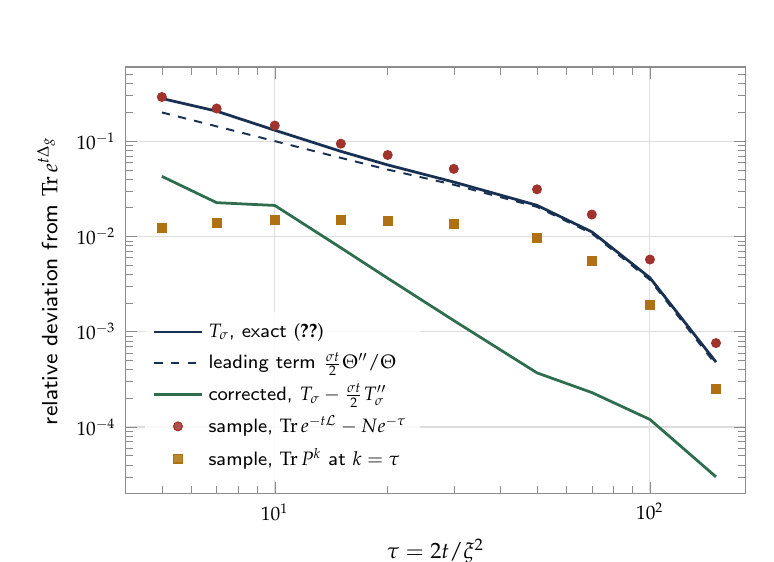
\begin{tikzpicture}
\begin{loglogaxis}[width=0.78\textwidth,height=70mm,xmin=4,xmax=180,ymin=2e-5,ymax=0.6,
  xlabel={$\tau=2t/\xi^2$},ylabel={relative deviation from $\Tr e^{t\Delta_g}$},
  xlabel style={font=\sffamily\footnotesize},ylabel style={font=\sffamily\footnotesize},
  ticklabel style={font=\sffamily\scriptsize},grid=major,grid style={rulegray!30},
  axis line style={rulegray},tick style={rulegray},
  legend style={font=\sffamily\scriptsize,draw=none,fill=white,fill opacity=0.85,text opacity=1,at={(0.03,0.03)},anchor=south west},legend cell align=left]
\addplot[ink,line width=1pt] coordinates {(5,0.28016) (7,0.20630) (10,0.13016) (15,0.07814) (20,0.05626) (30,0.03722) (50,0.02120) (70,0.01117) (100,0.00368) (150,0.00048)};
\addlegendentry{$T_\sigma$, exact \eqref{eq:Tsigma}}
\addplot[ink,dashed,line width=0.7pt] coordinates {(5,0.20000) (7,0.14286) (10,0.10000) (15,0.06669) (20,0.05027) (30,0.03485) (50,0.02040) (70,0.01074) (100,0.00350) (150,0.00045)};
\addlegendentry{leading term $\tfrac{\sigma t}{2}\Theta''/\Theta$}
\addplot[okgreen,line width=1pt] coordinates {(5,0.04270) (7,0.02260) (10,0.02113) (15,0.00760) (20,0.00364) (30,0.00131) (50,0.00037) (70,0.00023) (100,0.00012) (150,0.00003)};
\addlegendentry{corrected, $T_\sigma-\tfrac{\sigma t}{2}T_\sigma''$}
\addplot[only marks,mark=*,mark size=1.6pt,badred] coordinates {(5,0.29043) (7,0.22002) (10,0.14578) (15,0.09396) (20,0.07153) (30,0.05114) (50,0.03121) (70,0.01697) (100,0.00572) (150,0.00076)};
\addlegendentry{sample, $\Tr e^{-t\Lc}-Ne^{-\tau}$}
\addplot[only marks,mark=square*,mark size=1.6pt,warnamber] coordinates {(5,0.01215) (7,0.01393) (10,0.01482) (15,0.01483) (20,0.01443) (30,0.01338) (50,0.00967) (70,0.00552) (100,0.00189) (150,0.00025)};
\addlegendentry{sample, $\Tr P^k$ at $k=\tau$}
\end{loglogaxis}
\end{tikzpicture}
\caption{Relative deviation from the heat trace on the flat unit torus of dimension two, $\xi=0.05$. Lines: the exactly solvable case of Theorem~\ref{thm:rate}, evaluated by mode sums. Marks: one sample of $N=5000$ uniform points with the Gaussian profile. The continuous-time trace follows the law $d(d+2)/8\tau=1/\tau$; the trace in discrete time has no such term, and what remains for it is the sampling error of this sample. For $\tau\gtrsim70$ the time $t$ is no longer small and all deviations decrease faster, because the constant mode dominates. A single sample is not evidence for a rate.}\label{fig:rate}
\end{figure}

\begin{remark}[Machine-checked statements]\label{rem:lean}
The following parts of this appendix and of Theorems~\ref{thm:poisson} and~\ref{thm:trace} have been formalised and checked with the proof assistant Lean~4 (file \texttt{CorrelationsToGeometry.lean}, section~8), over an arbitrary ordered field with a function $\exp$ that satisfies $\exp(x+y)=\exp(x)\exp(y)$ and $\exp(x)\ge1+x$:
\begin{itemize}
\item for a row-stochastic matrix with nonnegative entries, $0\le\Tr P^k\le N$, and every partial sum of $\sum_kc_k\Tr P^k$ with weights $c_k\ge0$ lies between $c_0N$ and $N\sum_kc_k$ (the coefficientwise form of Theorem~\ref{thm:poisson});
\item for a list of numbers $s_a\le1$: $\sum_ae^{-\tau(1-s_a)}\le N$, monotonicity in $\tau$, the bound $e^{-\tau}(N+\tau m_1)\le\sum_ae^{-\tau(1-s_a)}$, the lower bound $Ne^{-\tau}$ under $m_1\ge0$, the second and third inequalities of \eqref{eq:chain} in the form of Jensen's inequality with uniform and with general weights, and the identity in \eqref{eq:twoterm};
\item the inequality $|e^{-x}-e^{-y}|\le|x-y|e^{-\min(x,y)}$ used for the low modes;
\item with the two Taylor bounds $\varphi(x)\le\tfrac12x^2e^{\max(x,0)}$ taken as hypotheses: the upper bound in \eqref{eq:twoterm} and the estimate $e^{-\tau}\sum_{s_a\le1-\kappa}\varphi(\tau s_a)\le\tfrac12\tau^2e^{-\kappa\tau}\sum_as_a^2$ for the high modes in the proof of Theorem~\ref{thm:trace}.
\end{itemize}
For Theorem~\ref{thm:rate} the estimates for a single mode are checked: $b_k\le a_k$; $a_k-b_k\le\frac{x^2}{2\tau}e^{-x/2}$ for $x\le\tau$, with the Taylor bound as hypothesis, and its sum over a finite list of low modes; and $e^{-\tau}(e^{\tau s}-1)\le\tau s\,e^{-\tau(1-s_0)}$ for $0\le s\le s_0$. For Proposition~\ref{prop:discrete}: $s^k\le e^{-k(1-s)}$ for $s\ge0$, and $s^{k+2}\le(1-\kappa)^ks^2$ for $0\le s\le1-\kappa$. For part (iii) of Theorem~\ref{thm:rate} and for Theorem~\ref{thm:corrected} the estimates of a low mode, $-\tfrac{x^3}{6\tau^2}e^{-x}\le a_k-b_k-\tfrac{x^2}{2\tau}b_k\le\tfrac{x^4}{8\tau^2}e^{-x/2}$ and $|a_k(1-z_k^2/2\tau)-b_k|\le(\tfrac12x^3+\tfrac14x^4)e^{-x/2}/\tau^2$, are checked, with the third-order Taylor bound of $e^{-u}$ as a further hypothesis, and so are their sums over an arbitrary finite family of low modes, with bounds that do not depend on the number of modes. For part (i) the exchange of the two sums is checked for finitely many modes and finitely many terms, $\sum_k\sum_{j\le m}c_js_k^j=\sum_{j\le m}c_j\sum_ks_k^j$, together with the one-sided inequality that every truncation of the Poisson series lies below the subtracted trace.

For Theorem~\ref{thm:corrected} the estimate of a high mode, $|e^{-\tau}[e^{\tau s}(1-\tfrac12\tau(1-s)^2)-1+\tfrac\tau2]|\le\tau s\,(2+\tfrac\tau2)\,e^{-\tau(1-s_0)}$ for $0\le s\le s_0\le1$, is checked as well. For Theorem~\ref{thm:profile} the estimates of a single mode are checked in the form used in the proof: a low mode in continuous time under (F1), given $|y|\le x/4$; a low mode in discrete time, where the expansion of $\ln s_k$ enters as a hypothesis; and the high modes in continuous and in discrete time under $|s_k|\le1-\delta$. For Theorem~\ref{thm:fixedxi} the two deterministic steps are checked: the bound $|\prod_la_l-\prod_lb_l|\le n\,\varepsilon M^{n-1}$ for the replacement of $p_N$ by $p$, and Step~3 in the form of a dominated convergence theorem for series.

\emph{The Taylor bounds.} In the statements above the Taylor bounds of the exponential function were hypotheses. They are derived in the same file for every Archimedean ordered field, from $\exp(x+y)=\exp(x)\exp(y)$ and $\exp(x)\ge1+x$ alone, by Riemann sums: $e^{(n+1)h}-e^{nh}=e^{nh}(e^h-1)$ is summed over $n$ and the step $h=x/N$ is sent to zero with the Archimedean property. This gives $e^x-1-x\le\tfrac12x^2e^{\max(x,0)}$, $1-u+\tfrac12u^2-\tfrac16u^3\le e^{-u}$ and $1+x+\tfrac12x^2\le e^x$ for $x,u\ge0$, so that in an Archimedean field all statements listed here hold without analytic hypotheses on the exponential function. With these bounds the estimate of a low mode in Proposition~\ref{prop:discrete}, $0\le e^{-kv}-(1-v)^k\le kv^2e^{-kv}$ for $0\le v\le\tfrac12$, is checked without any use of logarithms. In the same way the exponential series is treated: $0\le e^x-\sum_{j\le m}x^j/j!\le\frac{x^{m+1}}{(m+1)!}e^x$ for $x\ge0$ and $x^m/m!\to0$ are proven, hence the convergence of the series. With this the Poisson identity of Theorem~\ref{thm:rate}(i) is checked in the following form: for nonnegative $s_k$, if the sums $T=\sum_k(e^{-\tau(1-s_k)}-e^{-\tau})$ and $p_j=\sum_ks_k^j$ exist, then $\sum_{j\ge1}e^{-\tau}\tau^jp_j/j!=T$; and Theorem~\ref{thm:fixedxi}(ii) with Corollary~\ref{cor:torus} in the form: if $\Tr P^j\to p_j$ for every $j$, with a uniform bound, then the subtracted trace converges to $T$. No property of the exponential function other than the two stated ones and the Archimedean axiom is used. Also checked are the algebraic identities behind Proposition~\ref{prop:sphere} (the Taylor coefficients of $P_l(\cos\theta)$, the form \eqref{eq:sphereF1} and the expansion of $\sigma_\xi$) and the value $\beta=(d+2)/(d+4)$ for the ball.

\emph{Limits.} The proof assistant was used with its core library only, which contains no real numbers. Convergence of a sequence is therefore defined directly, for sequences in an arbitrary ordered field, and the following are proven in that setting, with the existence of the sums of the series that occur as hypotheses and without the use of completeness: a termwise inequality passes to the sums of two convergent series, and with it the estimates of the low modes in Theorems~\ref{thm:rate}(ii), (iii) and~\ref{thm:corrected} hold for infinitely many modes; the Poisson identity of Theorem~\ref{thm:rate}(i) as an equality of series, $\sum_jc_j\sum_ks_k^j=\sum_k\sum_jc_js_k^j$ for $c_j,s_k\ge0$; dominated convergence for series; and, combining the last two, the statement that if $\Tr P^j$ converges to the moments of the population walk for every $j$ and is bounded, then the subtracted trace converges to $T_\sigma$, which is Theorem~\ref{thm:fixedxi}(ii) together with Corollary~\ref{cor:torus}.

What is not formalised in these statements: the laws of large numbers of Steps~1 and~2 of Theorem~\ref{thm:fixedxi}, which enter as the hypothesis $\Tr P^j\to m_j^\infty$, and Proposition~\ref{prop:rateN}; the identification of the population operator on the torus with the heat kernel; the facts that remain hypotheses (the existence of the sums over infinitely many modes, which needs the completeness of the real numbers and bounds on the spectrum, and in Theorem~\ref{thm:profile}(ii) the expansion of the logarithm); Bernstein's inequality and the bound on Legendre polynomials in Propositions~\ref{prop:sphere} and~\ref{prop:spheregap}; Propositions~\ref{prop:oracle}, \ref{prop:estimated} and~\ref{prop:fixedxijump}, Lemma~\ref{lem:oraclemoments} and Theorems~\ref{thm:jointslow} and~\ref{thm:jointpoly} (the counting of walks, the spanning-tree bound and the probability estimates are not formalised; checked are $|\theta_{ij}|\le4\delta$ for $\delta\le\tfrac18$, $e^x\le1+2x$ for $0\le x\le\tfrac12$ and $(1+4\delta)^k-1\le8k\delta$ for $4k\delta\le\tfrac12$), of which otherwise only the expansion $|\prod_s(1+\theta_s)-1-\sum_s\theta_s|\le(1+a)^n-1-na$ and the two polynomial inequalities for $u\le\tfrac12$ in Proposition~\ref{prop:spheregap} are checked; Weyl's law and the bounds on $\Theta$ and $N_p$ that turn the sums over the modes into the right-hand sides of Theorems~\ref{thm:rate}--\ref{thm:profile}; Propositions~\ref{prop:ratereduction} and~\ref{prop:discrete} as a whole; and the probabilistic parts of Propositions~\ref{prop:bias} and~\ref{prop:variance} (moments, Bernstein's inequality, the expectations of the polynomial statistics, the Hoeffding decomposition), of which the algebra is checked: the expansion of $\gamma_i$ with the explicit remainder $R_i$, the sum of the four expectations to $\beta_k$, the difference between the graphs with and without self-loops, the sum of the pair kernels to $H_k$, and $\beta_k=\frac12H_k(0)$. Lemmas~\ref{lem:pgauss}, \ref{lem:consistency}, \ref{lem:degenerate}, \ref{lem:pibound} and~\ref{lem:kernelmatrix} are not formalised; of Proposition~\ref{prop:reduction} the algebra of the linearisation in Step~2 is checked, and of Corollary~\ref{cor:secondstage} the identity for the sum of $\theta^1_{ii}$ over the diagonal and the summation over the Poisson weights, and the counterexample that makes the second part of \textup{(F2)} in Theorem~\ref{thm:profile} necessary is checked as a negative control; of Theorem~\ref{thm:eigtorus} only the inequality $x^{k+1}-y^{k+1}\ge(k+1)y^k(x-y)$ for $0\le y\le x$, by which the eigenvalues are recovered from their powers; of Corollaries~\ref{cor:eigspace} and~\ref{cor:deloc} the inequality $e^{-u}-e^{-v}\ge e^{-v}(v-u)$ for $u\le v$ behind the separation of the powers, the step $\rho^2\|(1-\Pi)w\|^2\le\|(B-a)w\|^2$ in the coordinates of an eigenbasis, and the Cauchy--Schwarz inequality for finite sums with the resulting bound $u_a^2\le c^2\sum_iB_i^2$; and, as whole deductions with the non-formalised inputs as hypotheses: the induction of Step~4 of Theorem~\ref{thm:kernel} from the recursion \eqref{eq:kernel-rec} and a bound $S_k\le W_km_{k+1}$ (the consistency lemma enters only through this bound); the passage from part (i) to part (ii) of Theorem~\ref{thm:eigtorus}, that is $(k+1)\,a^{k+1}\sigma\,|\lambda^N_j-\lambda^{\mathrm{pop}}_j|\le2\eta$ from $|s_j^{k+1}-a^{k+1}|\le\eta\le\frac12a^{k+1}$; and Corollary~\ref{cor:deloc} from the eigenvalue equation, the symmetry of $S^k$ and a bound on the diagonal of $S^{2k}$; and of Theorem~\ref{thm:kernel} only the following: the telescoping identity of Step~1, for an arbitrary matrix and an arbitrary sequence of vectors; the inequality that turns \eqref{eq:kernel-rec} and a bound on $S_k$ into the bound on $D_{k+1}$, and the logic of the induction of Step~4, in which the hypothesis enters only as $D_l\le m_l$; the fact that a row-stochastic matrix does not increase the maximum of a vector, the bound of a weighted sum by the largest weight times the sum of the absolute values, and with it the statement that a recursion $v_{n+1}=Pv_n$ and an approximate solution with defects $\eta_n$ differ by at most the initial error plus $\sum\eta_n$.

Not formalised are the spectral theorem for $S$, which connects the matrix $e^{-t\Lc}$ with the sums over $s_a$, the convergence of the exponential series, the lower bound in \eqref{eq:twoterm}, the logarithmic convexity, and every statement that involves the manifold: Theorem~\ref{thm:eig}, Lemmas~\ref{lem:weights} and~\ref{lem:traces}, Weyl's law, and with them the limit \eqref{eq:tracesub} itself and Corollary~\ref{cor:subtractions}. The same file contains the algebraic statements of Section~\ref{sec:content} (Corollaries~\ref{cor:content}, \ref{cor:nextorder} and~\ref{cor:vanish}, Proposition~\ref{prop:relations}, and the values of Tables~\ref{tab:species} and~\ref{tab:models} for the continuum fields), with the entries of Table~\ref{tab:species} and of Proposition~\ref{prop:massterms} as inputs. It also contains the algebra of the symplectic spectrum used in Proposition~\ref{prop:twomode}: for the covariance matrix with the blocks $\big(\begin{smallmatrix}x_0&x\\x&x_0\end{smallmatrix}\big)$ and $\big(\begin{smallmatrix}p_0&p\\p&p_0\end{smallmatrix}\big)$ the product of the blocks has the eigenvalues $(x_0\pm x)(p_0\pm p)$, and an explicit symplectic matrix, a rotation by $45^\circ$ followed by two rescalings, brings the covariance matrix to $\operatorname{diag}(\nu_+,\nu_-,\nu_+,\nu_-)$ with $\nu_\pm^2=(x_0\pm x)(p_0\pm p)$; the square roots enter as hypotheses, and the statement that the entropy of a Gaussian state is the sum of $f$ over its symplectic eigenvalues is not formalised. A second file, \texttt{CorrelationsToGeometryReal.lean}, uses the library Mathlib (the version for Lean~4.29.0) and imports the first one unchanged. It proves that the real numbers are Archimedean in the sense used above and that the real exponential function has the two defining properties, so that the Taylor bounds, the convergence of the exponential series, the estimate of a low mode of the corrected estimator (Theorem~\ref{thm:corrected}) and the Poisson identity (Theorem~\ref{thm:rate}(i)) hold for the real exponential without a hypothesis on it; the existence of the sums over the modes remains a hypothesis there too. It also identifies the notion of limit used in the first file with convergence in the usual sense and states the Poisson identity with the infinite sums of Mathlib: if the sums over the modes exist, the partial sums of the Poisson series of the return moments converge to the subtracted trace. With the spectral theorem of Mathlib it further proves, for an arbitrary real symmetric matrix $S$ with eigenvalues $s_i$ and every real $\tau$, that $\Tr S^k=\sum_is_i^k$ and that $\sum_ie^{-\tau(1-s_i)}=\sum_{j\ge0}e^{-\tau}\frac{\tau^j}{j!}\Tr S^j$ as an infinite sum; together with $\Tr\exp(\tau(S-1))=\sum_ie^{-\tau(1-s_i)}$ for the matrix exponential this is the identity of Theorem~\ref{thm:poisson}, $\Tr e^{-t\Lc}=\sum_{j\ge0}e^{-\tau}\frac{\tau^j}{j!}\Tr S^j$, for every real symmetric matrix and without any hypothesis. For such matrices it also proves the lower bounds $e^{-\tau}(N+\tau\Tr S)\le\Tr e^{-t\Lc}$ for every real $\tau$ and $Ne^{-\tau}\le\Tr e^{-t\Lc}$ for $\tau\ge0$, $\Tr S\ge0$ (Theorem~\ref{thm:poisson}, Proposition~\ref{prop:heatbounds}). It proves that for symmetric nonnegative weights with positive degrees all eigenvalues of $S=D^{-1/2}WD^{-1/2}$ lie in $[-1,1]$, and from this the upper bound $\Tr e^{-t\Lc}\le N$. Of Theorem~\ref{thm:trace} it contains the deterministic part of the proof: for every real symmetric matrix $S$ with eigenvalues $s_i$, every $\tau\ge0$, $\kappa\le1$ and all real numbers $\mu_i$, with the low modes those with $1-s_i<\kappa$,
\[
\begin{aligned}
\Big|\Tr e^{-t\Lc}-Ne^{-\tau}-\sum_{\mathrm{low}}e^{-\mu_i}\Big|\le{}&\sum_{\mathrm{low}}\big|\tau(1-s_i)-\mu_i\big|\,e^{-\min(\tau(1-s_i),\mu_i)}+n_{\mathrm{low}}e^{-\tau}\\
&+\tau e^{-\tau}\Big|\sum_{\mathrm{high}}s_i\Big|+\frac{\tau^2}2e^{-\kappa\tau}\Tr S^2,
\end{aligned}
\]
without hypotheses, and a conditional form in which the first term is bounded by $\varepsilon\sum_{\mathrm{low}}\mu_ie^{-c\mu_i}$ under the hypotheses $|\tau(1-s_i)-\mu_i|\le\varepsilon\mu_i$ and $c\mu_i\le\tau(1-s_i)$ for the low modes. These are the four contributions in the proof of Theorem~\ref{thm:trace} with $\mu_i=t\lambda_i$. Three further steps of that proof are checked: the comparison term satisfies $\sum\mu_ie^{-c\mu_i}\le\frac2c\sum e^{-c\mu_i/2}$; for a row-stochastic matrix with entries in $[0,b]$ one has $\Tr P\le Nb$ and $\Tr P^2\le Nb$ (the deterministic part of Lemma~\ref{lem:traces}); the entries of the walk are at most $A\,q_{\max}/(Nq_{\min}^2)$ if the kernel has values in $[0,A]$ and the estimated normalisation lies in $[q_{\min},q_{\max}]$; and, with the probability theory of Mathlib, Hoeffding's inequality for the normalisation, $\mathbb P(|q_N(x)-q(x)|\ge s)\le2e^{-2Ns^2/A^2}$ at a fixed point, and uniformly: for independent points of a metric space, a kernel with values in $[0,A]$ that is $L$-Lipschitz in its first argument and a finite $r$-net, the probability that $|q_N(x)-q(x)|$ exceeds $s+2Lr$ for some point $x$, in particular for some sample point, is at most twice the size of the net times $e^{-2Ns^2/A^2}$ (the concentration step of Lemma~\ref{lem:weights} and of Proposition~\ref{prop:rateN}; the existence and the size of the net, the Lipschitz constant of $q$ and the identity $q(x)=\mathbb E\,k(x,X_j)$ are hypotheses there). These steps are assembled on a torus: for a compact abelian group with a translation-invariant metric and its invariant probability measure (the circle $\R/\mathbb Z$ is checked as an instance), independent points with this law and a kernel $k(x,y)=h(x-y)$ with $h$ measurable, $L$-Lipschitz, with values in $[0,A]$ and $q_0=\int h>0$, there is for every $r>0$ a number $M$ such that for all $N\ge1$ and all $s\ge0$ with $s+2Lr\le q_0/2$
\[
\mathbb P\Big(\Tr P>\frac{6A}{q_0}\ \text{ or }\ \Tr P^2>\frac{6A}{q_0}\Big)\le2M\,e^{-2Ns^2/A^2},
\]
without further hypotheses. This is Lemma~\ref{lem:traces} with its probability for Lipschitz kernels on a torus, where $A/q_0$ is of the order $\xi^{-d}$; the number $M$, the size of an $r$-net, is obtained from compactness and not quantified, so that the statement gives no rate in $\xi$. The same is proven for the flat torus $(\R/\mathbb Z)^d$ of every dimension with the product of the Haar measures, and, by the Borel--Cantelli lemma, in the almost sure form: for a fixed kernel, almost surely $\Tr P\le6A/q_0$ and $\Tr P^2\le6A/q_0$ for all large $N$. Two further elementary steps of the proof of Theorem~\ref{thm:trace} are checked: a finite set of lattice points $n\in\mathbb Z^d$ with $|n|^2\le m^2$ has at most $(2m+1)^d$ elements (the upper bound of Weyl's law on the flat torus, where the eigenvalues are $4\pi^2|n|^2$), and $\sum e^{-t\lambda_i}\le e^{-tb/2}\sum e^{-t\lambda_i/2}$ if all $\lambda_i\ge b$ (the contribution of the modes beyond the low ones). Not formalised, and therefore still resting on the written proofs alone: the eigenvalue estimates of Theorem~\ref{thm:eig}, which need the Laplace--Beltrami operator and the comparison of Dirichlet forms and for which the library offers no basis; Weyl's law on a general manifold, and on the torus the identification of the spectrum with the lattice; Lemma~\ref{lem:weights} for profile kernels on a general manifold (the size of the nets, a normalisation that depends on the point, kernels that are not Lipschitz); and the assembly of these parts into the limit \eqref{eq:tracesub}. Theorem~\ref{thm:trace} as a statement about random samples of a manifold is thus not machine-checked. Of Theorem~\ref{thm:kernel} the file contains the whole deterministic argument for matrices. For a matrix $P$ with nonnegative entries and unit row sums and kernels $0\le p_k\le\mu_k$ on the index set, let $D_k$ be the largest entry of $NP^k-p_k$. If the last step of the walk, the consistency of the defects in the mean and in the supremum, and the summation over the defects hold as hypotheses, then $D_l\le\mu_l$ for $1\le l\le K$ and $D_{j+2}\le(4d+(1+4d)W_{j+1})\,\mu_{j+2}$; the steps are the stability of $P$ in the supremum norm, the telescoping identity, the recursion \eqref{eq:kernel-rec} and the induction. Of Theorem~\ref{thm:eigtorus} it contains the deterministic part: Weyl's inequality for the eigenvalues of real symmetric matrices in decreasing order, $|a_j-b_j|\le\max_i\sum_l|A_{il}-B_{il}|$, which a search of the library did not find and which is therefore proven in the file by a count of dimensions; the fact that the eigenvalues of $S^k$ in decreasing order are the $k$-th powers of those of $S$ when these are nonnegative; and from them parts (i) and (ii) of the theorem, given a bound on the row sums of $S^{k+1}-Q$ and on the eigenvalues of $Q$. Of Lemma~\ref{lem:consistency} it contains the main term at fixed points. An inequality of Bernstein type, which the library does not have either, is proven: for independent centred random variables with $|X_i|\le b$ and $\sum\mathbb E X_i^2\le V$, $\mathbb P(\sum X_i\ge\varepsilon)\le\exp(-\varepsilon^2/(4V+2b\varepsilon))$; the classical denominator is $2V+\frac23b\varepsilon$, so that only constants change. With it, for independent points with a translation-invariant law on a commutative group and the convolution powers $p^{*m}$ of a bounded nonnegative kernel, $\sum_{j<N}p(x-X_j)\,p^{*m}(X_j-y)$ deviates from $N\,p^{*(m+1)}(x-y)$ by $\varepsilon$ or more with probability at most $2\exp(-\varepsilon^2/(4NMB\,p^{*(m+1)}(x-y)+2MB\varepsilon))$, where $M$ and $B$ bound $p$ and $p^{*m}$; the semigroup property enters as the definition of the convolution powers, and measurability of the integrand is a hypothesis. At a fixed kernel scale the chain is closed: for a compact abelian group with a translation-invariant metric and its invariant probability measure (the flat torus of every dimension is checked as an instance), independent points with this law and a measurable Lipschitz probability density $p$ with $0\le p\le M$, the estimate displayed below holds for all entries except on an event whose probability is bounded explicitly in terms of $N$, the tolerances and the sizes of two nets; no hypothesis on the walk remains if $p(0)>0$. With the Borel--Cantelli lemma this gives a limit theorem that is checked as a whole: for every fixed $k$ and every $\eta>0$, almost surely $\max_{a,i}|N(P^{k+1})_{ai}-p^{*(k+1)}(x_a-x_i)|\le\eta$ for all large $N$, the entrywise analogue of Theorem~\ref{thm:fixedxi}. The consistency of the walk with the exact normalisation holds uniformly over all pairs of points, with a bound of Hoeffding type (a net of the product space and the Lipschitz continuity of the convolution powers); a deterministic step passes from that walk to the sampled walk, $|\sum_jP_{bj}g_j-c|\le3\,\mathrm{dev}+11\,\delta\,c$ if the normalisation errors are at most $\delta\le\frac18$; and together they give, outside events whose probabilities are bounded, for all entries
\[
\begin{aligned}
\big|N(P^{k+1})_{ai}-p^{*(k+1)}(x_a-x_i)\big|&\le10\,\delta\,\big(p^{*(k+1)}(x_a-x_i)+E_k\big)+E_k,\\
E_k&=\sum_{m\le k}\big(3\,\mathrm{dev}_m+11\,\delta\,\mu_{m+1}\big).
\end{aligned}
\]
This is weaker than Theorem~\ref{thm:kernel}: the second term of the deterministic step lacks the factor $m^{-1/2}$ of Lemma~\ref{lem:consistency}, which comes from the Poincar\'e inequality for the Gaussian measure, so that $E_k$ grows like $k$ and not like $\sqrt k$, and the bounds carry no rate in the kernel scale. Not formalised at this stage of the file (several items of the following list are supplied, in a different form, by the statements described further below), so that Theorems~\ref{thm:kernel} and~\ref{thm:eigtorus} as statements about random samples are not machine-checked: Lemma~\ref{lem:pgauss}, that is, the facts on the heat kernel of the torus that bound $\mu_k$ and the sums; in Lemma~\ref{lem:consistency} the part with the normalisation errors, the sample points in place of fixed points and the union over the triples; of Lemma~\ref{lem:kernelmatrix} everything except its deterministic core; and the derivation of the hypotheses of the two deterministic theorems from these lemmas. The deterministic core of Lemma~\ref{lem:kernelmatrix} is in the file: for $Q=XX^{\mathsf T}$, if every absolute row sum of $X^{\mathsf T}X-\mathrm{diag}(a)$ is at most $\epsilon$, then each eigenvalue of $Q$ in decreasing order is within $\epsilon$ of the corresponding one of the numbers $a_f$, padded with zeros and arranged in decreasing order (\texttt{kernel\_matrix\_spectrum}); and for $X_{if}=\sqrt{a_f}\,v_{if}$ these row sums are at most $\eta\sqrt{a_f}\sum_g\sqrt{a_g}$ when the Gram matrix of the columns of $v$ is within $\eta$ of the identity entrywise (\texttt{gram\_row\_sums}). For the probabilistic input the file has the simultaneous concentration of the Gram matrix of finitely many bounded orthonormal functions of the sample (\texttt{gram\_concentration}, orthonormality as a hypothesis), the fact that a nontrivial character has mean zero under a translation-invariant probability measure (\texttt{character\_mean\_zero}), and the resulting orthogonality relations for products of real Fourier modes (\texttt{mode\_products}), which hold without hypotheses on the circle (\texttt{circle\_mode\_products}); and on the flat torus of every dimension for the characters $\prod_ie^{2\pi in_ix_i}$ (\texttt{flatTorus\_mode\_products}). The deterministic steps are assembled: from a Gram matrix within $\eta$ of the identity to the eigenvalues of the matrix of a kernel of finite rank (\texttt{finite\_rank\_kernel\_spectrum}), and from there, given the row sums of $S^{k+1}$ minus that matrix, to parts~(i) and~(ii) of Theorem~\ref{thm:eigtorus} (\texttt{eigtorus\_from\_gram}). For independent uniform points on the flat torus the Gram matrix of the sampled real modes $1$, $\sqrt2\,\mathrm{Re}\,\chi_n$, $\sqrt2\,\mathrm{Im}\,\chi_n$ concentrates without any hypothesis on the modes (\texttt{torusMode\_orthonormal}, \texttt{flatTorus\_gram\_whp}). The pair of real modes of a frequency reproduces $2\,\mathrm{Re}\,\chi_n(x-y)$ (\texttt{torusMode\_kernel}), and the position of a value among the ordered coefficients follows from two counts (\texttt{diag\_pad\_eigenvalue}). The row sums required by \texttt{eigtorus\_from\_gram} follow deterministically from an entrywise kernel bound, the normalisation and a bound on the tail of the Fourier series (\texttt{conj\_pow\_entry}, \texttt{row\_sums\_from\_kernel}). Not derived in the file are these three inputs themselves, in particular the kernel bound with its rate, and the two counts for the lattice points of the torus. Of Lemma~\ref{lem:pgauss} the file contains the pointwise inequalities for the Gaussian on the line behind (P1), (P3) and (P4) (\texttt{gauss\_scale\_mono}, \texttt{gauss\_gradient\_core}, \texttt{gauss\_product\_core}) and the quantitative part of (P2) in Fourier form: $\sum_{n\in\mathbb Z^d}e^{-c|n|^2}\le(1+\sqrt{\pi/c})^d$ with the corresponding bound for the tail over $|n|^2\ge R$ (\texttt{gauss\_tsum\_le}, \texttt{gauss\_tail\_sum\_le}), and, for the kernel defined by its Fourier series $p(x)=\sum_ne^{-c|n|^2}\,\mathrm{Re}\,\chi_n(x)$ on the flat torus, that its convolution powers are the same series with $c$ replaced by $(m+1)c$ and are bounded by $(1+\sqrt{\pi/((m+1)c)})^d$ (\texttt{cosSeries\_conv}, \texttt{heatTorus\_convPow}); with $c=2\pi^2\tau$ for the kernel $p^{(\tau)}$ of variance $\tau$ this is $\sup p^{(k\tau)}\le(1+(2\pi k\tau)^{-1/2})^d$; the kernel of the walk has $\tau=\xi^2$, which is twice the $\sigma$ of this appendix, and in the description of the file in this and the next paragraphs $\sigma$ stands for this $\tau=\xi^2$. The kernel defined by this series is nonnegative in every dimension (\texttt{heatTorus\_nonneg}), by Jacobi's transformation formula in one variable from Mathlib and the factorisation of a series over $\mathbb Z^d$ of products (\texttt{theta\_factor\_nonneg}, \texttt{hasSum\_pi\_prod}). It has mass one, is positive at the origin and Lipschitz with constant $2\pi(2/c)(1+\sqrt{2\pi/c})^d$ for the supremum metric of the torus (\texttt{heatTorus\_mass}, \texttt{heatTorus\_zero\_pos}, \texttt{heatTorus\_lipschitz}). With these facts the almost sure statement at a fixed scale holds for this kernel without any hypothesis (\texttt{heatTorus\_walk\_ae}): for independent uniform points on the flat torus of dimension $d$, every $k$ and every $\eta>0$, almost surely for all large $N$, $\max_{a,i}|N(P^{k+1})_{ai}-p_{(k+1)\sigma}(x_a-x_i)|\le\eta$, where $P$ is the walk of the sampled graph with self-loops and $p_s$ the heat kernel at time $s$ in its Fourier form. This is the entrywise counterpart of Theorem~\ref{thm:fixedxi} on the torus; it carries no rate in the kernel scale and is not Theorem~\ref{thm:kernel}. A quantitative version with explicit constants is also in the file (\texttt{heatTorus\_walk\_whp}), obtained with explicit nets of $m^d$ points on the torus: with $M=(1+\sqrt{\pi/c})^d$, $\delta=(\epsilon_n+2NL/m)/N$ and $e=3(\epsilon_c+2NL_*/m)/N+11\delta M$, the probability that some entry violates $|N(P^{k+1})_{ai}-p_{(k+1)\sigma}(x_a-x_i)|\le10\,\delta\,(p_{(k+1)\sigma}+ke)+ke$ is at most $2m^de^{-\epsilon_n^2/(2N(M/2)^2)}+2km^{2d}e^{-\epsilon_c^2/(2N(M^2/2)^2)}$, where $L$ and $L_*$ are explicit Lipschitz constants. This is a weak form of Theorem~\ref{thm:kernel}: it uses Hoeffding's inequality in place of Bernstein's, the uniform bound $M$ for all convolution powers, and an error linear in $k$; the regime of $(N,\xi)$ in which it is informative is smaller than that of the theorem and has not been worked out. Not in the file: the identification of the series with the periodised Gaussian as a formula, (P3)--(P5), and the sharp consistency estimate. Towards a statement on the eigenvalues of the sampled graph the file further contains: the matrix of this kernel at arbitrary points is positive semidefinite (\texttt{heatTorus\_quadform\_nonneg}), and the kernel is approximated uniformly, up to $e^{-cR/2}(1+\sqrt{2\pi/c})^d$, by its Fourier sum over the frequencies with $|n|^2<R$, written over a set of frequencies containing no pair $n,-n$ (\texttt{heatTorus\_truncation}, \texttt{heatTorus\_truncation\_half}); the truncated kernel is a sum over the real modes of such a set (\texttt{modeSet\_kernel}); and the deterministic steps from the entries of $P^{k+1}$ to parts~(i) and~(ii) of Theorem~\ref{thm:eigtorus} are composed into one statement that holds on the event where normalisation, consistency and Gram matrix are controlled (\texttt{eig\_sample\_det}). For the symmetric matrix $S=D^{-1/2}WD^{-1/2}$ of a graph with normalised weights the file has its conjugation to the walk, the bound $|\sqrt{D_i/D_l}-1|\le3\delta$ when the estimated normalisation is within $\delta\le\frac18$ of one, and that its eigenvalues lie in $[0,1]$ when the kernel matrix is positive semidefinite (\texttt{symGraph\_conj}, \texttt{graph\_degree\_bounds}, \texttt{sqrt\_ratio\_bound}, \texttt{symGraph\_eig\_nonneg}, \texttt{symGraph\_eig\_le\_one}). These facts and the truncation are inserted for the torus in \texttt{heatTorus\_eig\_det}: for arbitrary points $x_1,\dots,x_N$ on the flat torus at which the normalisation is within $\delta\le\frac18$ of one, the consistency errors are at most $\mathrm{dev}_m$ and the Gram matrix of the sampled modes is within $\eta$ of the identity, parts~(i) and~(ii) of Theorem~\ref{thm:eigtorus} hold for the $j$-th eigenvalue of $S$ with explicit error terms, where the comparison value $\alpha^{k+1}$ is characterised as the $j$-th largest of the coefficients $e^{-(k+1)c|n|^2}$ of the modes by two counts; no hypothesis on eigenvalues, symmetry or positivity remains. The probability of this event is bounded with the three concentration statements and the explicit nets (\texttt{heatTorus\_eig\_whp}, \texttt{heatTorus\_eig\_sample}): for independent uniform points on the flat torus, the two inequalities of parts~(i) and~(ii) for the $j$-th eigenvalue of $S$ fail with probability at most $2m^de^{-\epsilon_n^2/(2N(M/2)^2)}+2km^{2d}e^{-\epsilon_c^2/(2N(M^2/2)^2)}+2|F|^2e^{-(N\eta/2)^2/(2N)}$, where $F$ is the set of real modes used and the error terms are explicit in $\epsilon_n,\epsilon_c,\eta$, the grid parameter $m$, the truncation radius and $c$; the only hypotheses are those on the sample, inequalities between explicit numbers, and the two counts that characterise $\alpha^{k+1}$. This is a weak form of Theorem~\ref{thm:eigtorus} as a statement on random samples, with the same losses as the weak form of Theorem~\ref{thm:kernel} above; the regime of $(N,\xi)$ in which its inequalities can be satisfied has not been worked out, and Theorems~\ref{thm:kernel} and~\ref{thm:eigtorus} in the form stated in this appendix are not machine-checked. A sharper version of the entrywise bound uses Bernstein's inequality and the decaying bounds $B_j=(1+\sqrt{\pi/((j+1)c)})^d$ of the convolution powers (\texttt{uniform\_concentration\_bernstein}, \texttt{heatTorus\_walk\_bernstein}): the probability is then at most $2m^de^{-\epsilon_n^2/(4NM+2M\epsilon_n)}+\sum_{j<k}2m^{2d}e^{-\epsilon_c^2/(4NMB_jB_{j+1}+2MB_j\epsilon_c)}$, with $B_{j+1}$ in place of $M$ in the error term. It still lacks the factor $m^{-1/2}$ and the Gaussian weight of Lemma~\ref{lem:consistency}; it is inserted into the eigenvalue statement (\texttt{heatTorus\_eig\_sample\_bernstein}). The script \texttt{scripts/lean\_weak\_form\_regime.py} evaluates the hypotheses of that statement with its explicit constants for the first nonconstant eigenvalue and failure probability $0.1$, searching the free parameters on a grid: among powers of ten, the smallest sample size for which they can be met is $N=10^{10},10^{8},10^{7},10^{8}$ for $d=1$ and $\xi=0.5,0.3,0.2,0.1$, and $N=10^{11},10^{9},10^{9},10^{11}$ for $d=2$ and the same $\xi$ (with $k=0$, and $k=2$ in the last case). At these thresholds the statement only gives $|s_j-\alpha|\le\alpha/(k+1)$ up to a factor below one, so the machine-checked weak form is not vacuous but is far from the sample sizes of the numerical illustrations and from the regime of the theorems of this appendix. For the sharp form of Lemma~\ref{lem:consistency} the file so far contains only the first steps: the kernel defined by its Fourier series is the product over the coordinates of one-dimensional periodised Gaussians (\texttt{theta\_factor\_eq}, \texttt{heatTorus\_eq\_prod}; Poisson summation in one variable from Mathlib), (P1) holds for it (\texttt{heatTorus\_P1}), and the one-variable inequality behind (P5), the square root of a periodised Gaussian against the periodised Gaussian at twice the time, is proved (\texttt{perGauss\_sqrt}). (P4) is proved in one variable, $p_a(u)\,p_t(z-u)\le(2\pi a)^{-1/2}\big(\tfrac{t+2a}{t}\big)^{1/2}(\sqrt{4\pi a}+1)\,p_{t+2a}(z)$ for the one-dimensional periodised Gaussian (\texttt{gauss\_double\_sum}, \texttt{perGauss\_P4}, stated without division), together with the uniform bound $\sum_ne^{-b(n-s)^2}\le\sqrt{\pi/b}+1$ for all shifts $s$ (\texttt{gauss\_shift\_tsum\_le}). Taking products over the coordinates gives (P4) and (P5) for the kernel of the torus with explicit factors that depend on the times (\texttt{heatTorus\_P4}, \texttt{heatTorus\_P5}); the constants uniform in the time, as stated in Lemma~\ref{lem:pgauss}, are not derived. In place of the Gaussian Poincar\'e inequality, which Mathlib does not contain as far as a search of its sources shows, the file has the elementary inequality for the explicit variance of a Gaussian under a Gaussian on the line: for $0<\sigma\le s$, $\frac{e^{-z^2/(s+2\sigma)}}{2\pi\sqrt{s(s+2\sigma)}}-\frac{e^{-z^2/(s+\sigma)}}{2\pi(s+\sigma)}\le\frac\sigma s\cdot\frac4{\pi s}\,e^{-z^2/6s}$ (\texttt{gauss\_variance\_core}); the left-hand side is $\mathbb E\,\gamma_s(z+\sqrt\sigma Z)^2-(\mathbb E\,\gamma_s(z+\sqrt\sigma Z))^2$, which is proved as an identity between integrals over the line (\texttt{gauss\_conv\_core}, \texttt{gauss\_first\_moment}, \texttt{gauss\_second\_moment}, \texttt{gauss\_variance\_line}), and $\sigma/s=1/m$ is the factor of the lemma. For the periodised function $g=\sum_n\gamma_s(\cdot+n)$ in one variable, each term of the sum over pairs of lattice points that makes up the variance is bounded by $\frac\sigma s\cdot\frac4{\pi s}\,e^{-k^2/12s}e^{-(x+n)^2/12s}$ with $k=n-n'$ (\texttt{pair\_variance\_term}), and the sum of these bounds is at most $(1+\sqrt{12\pi s})\sum_ne^{-(x+n)^2/12s}$ times that factor, a multiple of the periodised Gaussian at time $6s$ (\texttt{pair\_variance\_sum}). The integral of a single pair, $\int\gamma_\sigma(x-y)\gamma_s(y+a)\gamma_s(y+b)\,\dd y$, and the corresponding product of first moments are evaluated in closed form (\texttt{gauss\_pair\_integral}, \texttt{gauss\_first\_moment\_shift}, \texttt{gauss\_first\_pair}), so that the terms bounded in \texttt{pair\_variance\_term} are identified. The exchange of integral and series is carried out (\texttt{per\_first\_moment}, \texttt{per\_second\_moment}), which gives the variance bound in one variable as a statement on integrals over the line (\texttt{per\_variance\_line}): for $0<\sigma\le s$ and $g=\sum_n\gamma_s(\cdot+n)$,
\[
\int_{\R}\gamma_\sigma(x-y)\,g(y)^2\,\dd y-\Big(\int_{\R}\gamma_\sigma(x-y)\,g(y)\,\dd y\Big)^2\le\frac\sigma s\cdot\frac4{\pi s}\,\big(1+\sqrt{12\pi s}\big)\sum_{n\in\mathbb Z}e^{-(x+n)^2/12s}.
\]
This is the bound \eqref{eq:cons-v} for $d=1$ with the factor $\sigma/s=1/m$, obtained without the Gaussian Poincar\'e inequality and with a constant that depends on $s$ through $1+\sqrt{12\pi s}$. The unfolding of an integral over the circle into an integral over the line, $\int_{\mathbb T}\Gamma F=\int_{\R}\gamma(y)F(y\bmod1)\,\dd y$ for $\Gamma(x)=\sum_n\gamma(x+n)$, is also in the file (\texttt{line\_unfold}, \texttt{circle\_unfold}). With it the variance bound is transferred to the circle (\texttt{circle\_gauss\_integral}, \texttt{circle\_variance}): for the heat kernels $P_\sigma,P_s$ of the circle with $0<\sigma\le s$, $\int_{\mathbb T}P_\sigma(x-u)P_s(u-w)^2\,\dd u-\big(\int_{\mathbb T}P_\sigma(x-u)P_s(u-w)\,\dd u\big)^2$ is at most the right-hand side of the display above at the point $x-w$, and that right-hand side equals $\frac\sigma s\cdot\frac4{\pi s}(1+\sqrt{12\pi s})\sqrt{12\pi s}\,P_{6s}(x-w)$ (\texttt{circle\_variance\_weight}). This is \eqref{eq:cons-v} on the torus of dimension one, with the weight $p^{(6s)}$ of the lemma. The bound is extended to the flat torus of every dimension (\texttt{torus\_variance}), using that kernel and measure are products over the coordinates, the semigroup on the circle and an elementary inequality for the difference of two products (\texttt{heatTorus\_eq\_prod\_pC}, \texttt{flatTorus\_integral\_prod}, \texttt{circle\_first\_moment}, \texttt{prod\_sub\_prod\_le}): for $0<\sigma\le s$,
\[
\int_{\M}p^{(\sigma)}(x-y)\,p^{(s)}(y-w)^2\,\dd y-\Big(\int_{\M}p^{(\sigma)}(x-y)\,p^{(s)}(y-w)\,\dd y\Big)^2\le d\,\varepsilon\,\alpha^{d-1}\,p^{(6s)}(x-w),
\]
with $\varepsilon=\frac\sigma s\cdot\frac4{\pi s}(1+\sqrt{12\pi s})\sqrt{12\pi s}$ and $\alpha=\big(1+(2\pi s)^{-1/2}\big)\big(6s/(\sigma+s)\big)^{1/2}$. This is the variance bound \eqref{eq:cons-v} in every dimension, with the factor $\sigma/s=1/m$ and the weight $p^{(6s)}$, proved without the Gaussian Poincar\'e inequality; its constants depend on $s$ and are bounded as in the lemma only for $s$ in a bounded range (for $s\le1$, $\varepsilon\alpha^{d-1}\le C_d\,\frac\sigma s\,s^{-d/2}$, which is not derived in the file). The step ``given $x_b$ and $x_i$'' of the proof is available as a statement on independent random variables: a bound that holds for every fixed value of one of two independent variables holds for the pair, in particular for two disjoint parts of an independent sample (\texttt{indep\_cond\_bound}, \texttt{sample\_cond\_bound}). The other ingredients of that step are also in the file: Bernstein's inequality in two-sided form for a function of independent points (\texttt{bernstein\_two\_sided\_fn}), the semigroup property on the torus and the identity $\int p^{(\sigma)}(x-y)\,(p^{(s)}(y-w)-c)^2\,\dd y=\int p^{(\sigma)}(x-y)\,p^{(s)}(y-w)^2\,\dd y-c^2$ for $c=p^{(\sigma+s)}(x-w)$ (\texttt{torus\_first\_moment}, \texttt{torus\_centered\_second}). They are combined into the Bernstein step at fixed points (\texttt{heat\_consistency\_fixed}): for independent uniform points $X_j$ on the torus, fixed $x,w$, $0<\sigma\le s$ and $Y(z)=p^{(\sigma)}(x-z)\big(p^{(s)}(z-w)-p^{(\sigma+s)}(x-w)\big)$, if $|Y|\le B$ and $p^{(\sigma)}\le M_\sigma$ then $\mathbb P\big(|\sum_{j\in T}Y(X_j)|\ge\epsilon\big)\le2\exp\big(-\epsilon^2/(4|T|M_\sigma V+2B\epsilon)\big)$ for every finite index set $T$, where $V=d\,\varepsilon\,\alpha^{d-1}p^{(6s)}(x-w)$ is the bound of the display above; the bound $B$ is a hypothesis of this statement, and it is supplied by (P4) in the form $|Y(z)|\le K^d\,p^{(s+2\sigma)}(x-w)\,(2\pi(s+2\sigma))^{d/2}+M_\sigma\,p^{(\sigma+s)}(x-w)$ with $K=(2\pi\sigma)^{-1/2}(2\pi s)^{-1/2}(\sqrt{4\pi\sigma}+1)$ (\texttt{heat\_Y\_bound}); the kernel is strictly positive (\texttt{heatTorus\_pos}). The passage from fixed points to two sample points is available in general form (\texttt{cond\_pair\_bound}): if $\mathbb P\big(\theta(x,w)\le|\sum_{j\in T}Y(x,w,X_j)|\big)\le q$ for all fixed $x,w$, with a threshold $\theta$ that may depend on the two points, then the same holds with $x=X_b$, $w=X_i$ for indices $b\ne i$ outside $T$. Applied to the Bernstein step, with the bound from (P4) inserted and the threshold chosen so that the exponent is $L$, this gives estimate (ii) of the lemma for one pair of sample points and one index set (\texttt{heat\_consistency\_pair}): for indices $b,i$ outside a finite index set $T$,
\[
\mathbb P\Big(\Big|\sum_{j\in T}Y(X_b,X_i,X_j)\Big|\ge2\,B(X_b-X_i)\,L+2\sqrt{|T|\,M_\sigma\,V(X_b-X_i)\,L}\Big)\le2e^{-L},
\]
where $V(u)=d\,\varepsilon\,\alpha^{d-1}p^{(6s)}(u)$ and $B(u)$ is the bound from (P4) displayed above. This is the content of the paragraph ``Bernstein'' of the proof, with constants that depend on $\sigma$ and $s$. The union over the pairs is taken (\texttt{heat\_consistency\_all\_pairs}): with probability at least $1-2N^2e^{-L}$ the bound holds for all $b,i<N$ simultaneously, the sum running over $j<N$, $j\notin\{b,i\}$ and $|T|$ replaced by $N$; and over the numbers of steps $1\le m\le K$ with $s=m\sigma$, at the cost of a factor $K$ in the probability (\texttt{heat\_consistency\_all\_steps}). For the term $A$ of the proof the file has the moments of the summand, $\int Y^2\le M_\sigma V$ and $\int|Y|\le(M_\sigma V)^{1/2}$, and the Bernstein step for $|Y|-\mathbb E|Y|$ at fixed points (\texttt{heatY\_sq\_integral\_le}, \texttt{heatY\_abs\_integral\_le}, \texttt{heat\_abs\_consistency\_fixed\_all}), and its transfer to a pair of sample points with the same threshold and probability as for $Y$ (\texttt{heat\_abs\_consistency\_pair}), and the union over the pairs and the numbers of steps as for $Y$ (\texttt{heat\_abs\_consistency\_all\_steps}). The deterministic steps towards the defect are in the file as separate statements: the splitting \eqref{eq:cons-split} in the form $|h|\le(|S_1|+\eta A)/r$ for normalisation factors within $\eta$ of one (\texttt{defect\_split}), and the two inequalities that restore the terms $j=b$ and $j=i$ (\texttt{abs\_sum\_le\_erase2}, \texttt{sum\_abs\_le\_erase2}). They are combined into a deterministic bound for the defect (\texttt{defect\_from\_bounds}): if the sum of $Y_j$ and the centred sum of $|Y_j|$ over $j\notin\{b,i\}$ are at most $\theta$ in absolute value, $|Y_b|,|Y_i|\le B$, the normalisation factors are within $\eta$ of one and $r\ge r_0$, then $|h|\le\big((\theta+2B)+\eta(Ne+\theta+2B)\big)/(Nr_0)$ with $e=\mathbb E|Y|$. For the sampled graph on the torus this gives, for points at which the estimated normalisations are within $\delta\le\frac12$ of one and the two Bernstein bounds hold for the pair $(b,i)$, the bound $|h^{(i)}_m(b)|\le3\big((\theta+2B)+2\delta(NV^{1/2}+\theta+2B)\big)/N$ for the one-step defect (\texttt{heat\_defect\_det}). Combined with the probabilities of the events this is estimate (ii) of the lemma with explicit constants that depend on the times (\texttt{heat\_defect\_whp}): except on an event of probability at most $p_n+4KN^2e^{-L}$, where $p_n$ is the probability of the normalisation event, the displayed bound holds for all $1\le m\le K$ and all $b,i<N$; and $p_n\le2g^de^{-\epsilon^2/(4NM+2M\epsilon)}$ for the explicit net of $g^d$ points (\texttt{heat\_normalisation\_whp}), so that the estimate holds for random samples with no hypothesis beyond those on the sample and inequalities between explicit numbers (\texttt{heat\_defect\_sample}). The term $S_2$ of the proof is contained in these statements through the factor $2\delta$, and the defect bounded there is identified with the expression $(Pg)(x_b)-p_{m+1}(x_b-x_i)$ for the walk matrix of the sampled graph (\texttt{walk\_defect\_eq}), the form in which the deterministic recursion uses it; the bound for the defect is at most its version with every kernel value replaced by the uniform bound of the kernel (\texttt{heatDefBound\_le\_sup}), which is the supremum bound required by the recursion. For the bound in the mean over the points, the bound for the defect is written as a linear function, with nonnegative coefficients, of $p^{(s+2\sigma)}(u)$, $p^{(\sigma+s)}(u)$ and $p^{(6s)}(u)^{1/2}$, compatible with finite sums and monotone (\texttt{heatDefBound\_eq\_num}, \texttt{heatDefNum\_sum}, \texttt{heatDefNum\_mono}); with the Cauchy--Schwarz inequality for a sum of square roots this bounds the sum of the defect bounds over the sample points once the sums of the three kernels over the points are at most $N(1+\delta_3)$ (\texttt{sum\_sqrt\_le}, \texttt{heat\_defect\_mean\_det}), and these sums are controlled by the normalisation event at the three times, which is estimate (iii) with the error of the normalisation in place of $9\delta'$ (\texttt{norm\_event\_sum}). The last step of the walk, $|NP_{bi}-K_{bi}|\le4\delta K_{bi}$ for estimated normalisations within $\delta\le\frac18$ of one, is proved for the walk matrix itself (\texttt{walk\_last\_step}). In the statements of the file described from here on, $\sigma$ denotes the parameter of the file, which is the variance $\xi^2$ of the Gaussian kernel, that is, twice the $\sigma$ of this appendix, and $p_{l\sigma}$ is the kernel after $l$ steps. These statements are inserted into the deterministic recursion (\texttt{kernel\_theorem\_matrix}, whose hypotheses on the defects are now required only for fewer than $K$ steps), which gives the recursion of Theorem~\ref{thm:kernel} for the sampled walk on the torus, first for points that satisfy the three kinds of estimates (\texttt{heat\_kernel\_sharp\_det}, \texttt{heat\_kernel\_sharp\_entries}) and then for independent uniform points (\texttt{heat\_kernel\_sharp\_whp}, \texttt{heat\_kernel\_sharp\_sample}): except on an event of probability at most $(2+4K)\,2g^de^{-\epsilon^2/(4NM+2M\epsilon)}+4KN^2e^{-L}$, for all $1\le l\le K$ and all $a,i$, $|NP^l(a,i)-p_{l\sigma}(x_a-x_i)|\le\mu_l$, and $|NP^{j+2}(a,i)-p_{(j+2)\sigma}(x_a-x_i)|\le(4\delta+(1+4\delta)W_{j+1})\mu_{j+2}$ for $j+1<K$, where $\mu_l=(1+(2\pi l\sigma)^{-1/2})^d$ and $\delta=(\epsilon+2N\,\mathrm{Lip}/g)/N\le\frac18$. This statement has no hypothesis on events; it has two hypotheses that are inequalities between explicit numbers: $4\delta+(1+4\delta)W_{j+1}\le1$, and that $W_{j+1}\mu_{j+2}$ dominates the sum over $m<j$ of the smaller of two bounds for the transported defect $P^{j-m}h_{m+1}$, namely $2\mu_{j-m}$ times the mean bound for the defect and the supremum bound for the defect, plus the supremum bound at step $j+1$. The choice between the two bounds is that of Step~3 of the proof; it uses that the walk matrix is row-stochastic (\texttt{kernel\_theorem\_matrix\_min}, \texttt{walkMatrix\_row\_sum}). The two numerical hypotheses were evaluated with the constants of the file (\texttt{scripts/lean\_sharp\_form\_regime.py}; failure probability $0.1$, $N$ restricted to powers of ten, so the values are upper bounds for the thresholds): they hold for $K=16$ steps from $N=10^{8}$, $10^{9}$, $10^{9}$ in $d=1$ for $\xi=0.3$, $0.2$, $0.1$, from $N=10^{10}$, $10^{10}$, $10^{11}$ in $d=2$ and from $N=10^{11}$, $10^{11}$, $10^{12}$ in $d=3$; for $K=\xi^{-2}=100$ steps and $\xi=0.1$ from $N=10^{10}$, $10^{12}$, $10^{13}$ in $d=1,2,3$. The smallest admissible $W_K$ is then between $2\cdot10^{2}$ and $5\cdot10^{3}$ times $\delta'\sqrt K$; for $K=16$ this factor is between $347$ and $355$ in $d=1$ for the three values of $\xi$, between $930$ and $1050$ in $d=2$ and between $2100$ and $2800$ in $d=3$, which is compatible with a bound $W_k\le C\delta'\sqrt k$ but does not prove one. So the statement is not empty, but its constants are far from those needed at the sample sizes of the numerical illustrations. The kernel bound is also carried over to the eigenvalues (\texttt{eig\_sample\_det\_kern}, \texttt{heatTorus\_eig\_det\_kern}, \texttt{heatKernelSharp\_kern}, \texttt{heat\_eig\_sharp\_whp}, \texttt{heat\_eig\_sharp\_sample}): for independent uniform points, with $k=j'+1<K$ steps and $D=(4\delta+(1+4\delta)W_{j'+1})\mu_{j'+2}$ in place of the kernel error of the weak form, the two inequalities of Theorem~\ref{thm:eigtorus}(i),(ii) for the $j$-th eigenvalue of $S$ fail with probability at most $(3+4K)\,2g^de^{-\epsilon^2/(4NM+2M\epsilon)}+4KN^2e^{-L}+2|F|^2e^{-(N\eta/2)^2/(2N)}$; besides the two numerical hypotheses of the kernel statement it requires the inequalities on the tail of the Fourier series and on the size of the error against $\alpha^{k+1}$, and the two counts that place $\alpha^{k+1}$ among the coefficients of the modes, as in the weak form. The numerical hypotheses of this eigenvalue statement have not been evaluated. In the bound for the defect the first absolute moment of $Y$ enters as $\int|Y|\le V^{1/2}$, by the Cauchy--Schwarz inequality with respect to the probability density $p^{(\sigma)}(x-\cdot)$ (\texttt{heatY\_abs\_integral\_sharp}), and the mean of $p^{(6s)}(u)^{1/2}$ over the sample is bounded by the smaller of the Cauchy--Schwarz bound and the bound through (P5) in the form $p^{(6s)}(u)^{1/2}\le q\,p^{(12s)}(u)$ with $q=(2(12\pi s)^{1/2})^{d/2}$ (\texttt{heatTorus\_sqrt\_le}, \texttt{heat\_defect\_mean\_det\_min}); the normalisation event is therefore used at the four times $m\sigma+2\sigma$, $\sigma+m\sigma$, $6m\sigma$, $12m\sigma$, which is the origin of the factors $4K$ in the probabilities above. Finally the summation of Step~4 is carried out in the file, for kernel time $\sigma\le1$ and $K\sigma\le1$. The coefficients of the bound for the defect are bounded in closed form for $\sigma\le s=m\sigma\le1$ (\texttt{heatKB\_le}, \texttt{heatCV\_le}, \texttt{heatCV\_le\_mu}, \texttt{heatCV\_heatQ}); this gives a bound $a/\sqrt m$ for the mean of the defect bound and $b\,\mu_m/\sqrt m$ for its supremum (\texttt{heatEtaBar\_le}, \texttt{heatDefSup\_le}), with
\[
a=3(1+\delta)\big((1+2\delta)(\theta+2\sqrt{ML/N}\,r)+2\delta r\big),\qquad b=3\big((1+2\delta)(\theta+2\sqrt{ML/N}\,r')+2\delta r'\big),
\]
where $r,r'$ depend only on $d$ and $\theta$ is any number with $(2L+2)(k_\sigma+M)\sqrt K\le\theta N$, $k_\sigma=\big((2\pi\sigma)^{-1/2}(\sqrt{4\pi}+1)\sqrt3\big)^d$. With $\mu_l\le2^d\mu_k$ for $k\le4l$ (\texttt{heatMu\_doubling}) and $\sum_{m\le k}m^{-1/2}\le2\sqrt k$ the summation hypothesis holds with $W_k=2\cdot2^d\max(2a,b)\sqrt k$ (\texttt{kernel\_sum\_bound}, \texttt{heat\_hsum\_closed}). The resulting statement (\texttt{heat\_kernel\_rate\_sample}) is: for independent uniform points on the flat torus, $\sigma\le1$, $K\sigma\le1$, $\delta\le\frac18$, and under the two inequalities $(2L+2)(k_\sigma+M)\sqrt K\le\theta N$ and $4\delta+(1+4\delta)W_K\le1$, except on an event of probability at most $(2+4K)\,2g^de^{-\epsilon^2/(4NM+2M\epsilon)}+4KN^2e^{-L}$,
\[
\big|N(P^{k})_{ai}-p_{k\sigma}(x_a-x_i)\big|\le\big(4\delta+(1+4\delta)\,2\cdot2^d\max(2a,b)\sqrt{k-1}\big)\,\mu_k\qquad(2\le k\le K,\ \text{all }a,i),
\]
and the corresponding statement for the eigenvalues is \texttt{heat\_eig\_rate\_sample}. This has the form of the estimate of Theorem~\ref{thm:kernel} with the factor $\sqrt k$ and an error that is linear in $\delta$, $\sqrt{ML/N}$ and $\theta$, machine-checked with the standard axioms only. Evaluated with its constants (same script, second table; $K\sigma\le1$), its two inequalities hold from $N=10^{10}$ to $10^{12}$ in $d=1$, $10^{14}$ to $10^{16}$ in $d=2$ and $10^{17}$ to $10^{19}$ in $d=3$ for $\xi\in\{0.3,0.2,0.1\}$ and $K$ between $4$ and $\xi^{-2}$, and $W_K/(\delta'\sqrt K)$ lies between $6.4\cdot10^{3}$ and $7.0\cdot10^{3}$ in $d=1$, $1.3\cdot10^{5}$ and $1.5\cdot10^{5}$ in $d=2$, $2.5\cdot10^{6}$ and $2.7\cdot10^{6}$ in $d=3$ in all these configurations. The free parameters are then fixed (\texttt{heat\_kernel\_rate\_prob}, \texttt{heat\_kernel\_rate\_explicit}): with $T=\log\big((2+4K)\,2g^dN^3\big)$, $L=\log(4KN^5)$, $\delta=6\sqrt{MT/N}$ and $\theta=(2L+2)(k_\sigma+M)\sqrt K/N$, under the three inequalities $2N\,\mathrm{Lip}/g\le3\sqrt{NMT}$, $6\sqrt{NMT}\le N/8$ and $4\delta+(1+4\delta)W_K\le1$, the displayed bound holds for all $2\le k\le K$ and all entries except on an event of probability at most $2/N^3$. Evaluated with the smallest admissible $g$ (same script, third table), the three inequalities hold from $N=10^{11}$ to $10^{13}$ in $d=1$, $10^{14}$ to $10^{17}$ in $d=2$ and $10^{17}$ to $10^{20}$ in $d=3$ for the same $\xi$ and $K$; there $\delta$ is between $11.4$ and $13.4$ times $\delta'$ and $W_K/(\delta'\sqrt K)$ is between $1.7\cdot10^{4}$ and $1.8\cdot10^{4}$ in $d=1$, $3.3\cdot10^{5}$ and $3.5\cdot10^{5}$ in $d=2$, $5.5\cdot10^{6}$ and $5.8\cdot10^{6}$ in $d=3$. The bound is then expressed through $\delta'$ (\texttt{heat\_kernel\_rate\_paper}): for $\sigma\le1$, $K\sigma\le1$, $1\le K\le N$, $N\ge12$ and $\delta'=\sqrt{M\log N/N}$, where in the file $M=(1+(2\pi\sigma)^{-1/2})^d$ is the uniform bound $\mu_1$ of the kernel and not $p(0)$ as in this appendix, so that this $\delta'$ exceeds the $\delta'$ of the appendix by a factor of at most $(1+\sqrt{2\pi}\,\xi)^{d/2}$, and where $\mathrm{Lip}=\frac{2}{\pi\sigma}(1+(\pi\sigma)^{-1/2})^d$ is the Lipschitz constant of the kernel proved in the file (supremum metric of the torus), under the two inequalities $2\,\mathrm{Lip}\le3\sqrt{NM\log N}$ and $C\,\delta'\sqrt K\le1$, except on an event of probability at most $2/N^3$,
\[
\big|N(P^{k})_{ai}-p_{k\sigma}(x_a-x_i)\big|\le C\,\delta'\,\sqrt k\;\mu_k\qquad(2\le k\le K,\ \text{all }a,i),
\]
with an explicit constant $C$ that depends only on $d$ (\texttt{rateCfin}; its value is $4.5\cdot10^{4}$, $8.5\cdot10^{5}$, $1.4\cdot10^{7}$ for $d=1,2,3$, and the two inequalities hold from $N=10^{12}$ to $10^{14}$, $10^{15}$ to $10^{17}$, $10^{18}$ to $10^{21}$ for the same $\xi$ and $K\in\{4,\lfloor\xi^{-2}\rfloor\}$; same script, fifth table). This has the form of the estimate of Theorem~\ref{thm:kernel}, with the grid parameter $g=N$. Since $\mu_k\le(1+\sqrt{2\pi})^d\,p_{k\sigma}(0)$ for $k\sigma\le1$ (\texttt{heatMu\_le\_m}; the kernel at the origin is at least $(2\pi k\sigma)^{-d/2}$), the same bound holds with $m_k=p_{k\sigma}(0)$ in place of $\mu_k$ and the constant $C(1+\sqrt{2\pi})^d$ (\texttt{heat\_kernel\_rate\_paper\_m}). For the eigenvalues the two counts are proved for the first shell (\texttt{mode\_counts\_shell}, \texttt{heat\_eig\_rate\_shell}): if $|n|^2\ge r>0$ on the set $H$ of frequencies and $E\subset H$ is the set where $|n|^2=r$, then for $1\le j\le2|E|$ (here and below the index $j$ of the file counts the eigenvalues in decreasing order from zero, so that it corresponds to $s_{j+1}$ in the numbering of this appendix) the eigenvalue statement holds with $\alpha=e^{-2\pi^2\sigma r}$ and no hypothesis on the position of $\alpha^{k+1}$ among the coefficients. The same holds for every shell below the cut-off of $H$ (\texttt{mode\_counts\_general}, \texttt{heat\_eig\_rate\_shells}): for $r>0$ and all indices $j$ with $1+2\,\#\{n\in H:|n|^2<r\}\le j\le2\,\#\{n\in H:|n|^2\le r\}$, which are the eigenvalues belonging to the shell $|n|^2=r$ counted with multiplicity when $H$ contains one of $n,-n$ for every nonzero frequency up to that shell. The passage from $|s_j-\alpha|$ to the eigenvalue $(1-s_j)/\tau$ of the graph Laplacian is a separate elementary statement (\texttt{eig\_lambda\_form}). Finally the eigenvalue statement is available uniformly in the step and in the index on one event (\texttt{heat\_eig\_uniform\_det}, \texttt{heat\_eig\_uniform\_sample}): in the situation of the kernel statement in the form $D_k\le C\delta'\sqrt k\,\mu_k$, with a normalisation tolerance $\epsilon$, $\delta=(\epsilon+2N\,\mathrm{Lip}/g)/N\le\frac18$, a set $H$ of frequencies with cut-off $R$ and a tolerance $\eta$ for the Gram matrix, except on an event of probability at most $2/N^3+2g^de^{-\epsilon^2/(4NM+2M\epsilon)}+2|F|^2e^{-(N\eta/2)^2/(2N)}$ the following holds simultaneously for all $2\le k\le K$, all $r>0$ and all indices $j$ of the shell $|n|^2=r$: if $2(e_k+\eta\sum_g\sqrt{a_g})\le\alpha^k$ with $\alpha=e^{-2\pi^2\sigma r}$ and $e_k=3\delta(M_k+D_k)+D_k+t_k$, where $M_k$ is the uniform bound of the kernel after $k$ steps and $t_k$ the tail of its Fourier series beyond $|n|^2\ge R$, then
\[
\big|s_j^k-\alpha^k\big|\le e_k+\eta\sum_g\sqrt{a_g},\qquad k\,\alpha^k\,|s_j-\alpha|\le2\Big(e_k+\eta\sum_g\sqrt{a_g}\Big).
\]
This is part (i) of Theorem~\ref{thm:eigtorus} and the first inequality of \eqref{eq:eig-step}, for the frequencies of $H$, with the sum $\eta\sum_g\sqrt{a_g}$ and the tail $t_k$ in place of the term $C\sqrt{\log N/N}\,m_k$ of Lemma~\ref{lem:kernelmatrix}. The sum is bounded, $\sum_g\sqrt{a_g}\le1+2\big(1+(\pi k\sigma)^{-1/2}\big)^d$ (\texttt{mode\_sqrt\_sum\_le}), and on the same event the statement is brought into the form of part (ii) (\texttt{lambda\_from\_power}, \texttt{heat\_eig\_lambda\_sample}): with $\tau=\sigma/2$, which is the $\sigma$ of this appendix, and $\lambda=4\pi^2r$, simultaneously for all $2\le k\le K$, all $r>0$ with $k\tau\lambda\le1$ and all indices $j$ of the shell, if $2E_k\le e^{-1}$ then
\[
\Big|\frac{1-s_j}{\tau}-\frac{1-e^{-\tau\lambda}}{\tau}\Big|\le\frac{2e\,E_k}{k\,\tau},\qquad E_k=e_k+\eta\Big(1+2\big(1+(\pi k\sigma)^{-1/2}\big)^d\Big).
\]
This is the second inequality of \eqref{eq:eig-step} with an explicit error; the step $k$ is a free parameter subject to $k\tau\lambda\le1$. The error is then expressed through $\delta'$ and the step is restricted to $\frac12\le k\tau\lambda\le1$ (\texttt{eig\_err\_closed}, \texttt{eig\_closed\_bound}, \texttt{heat\_eig\_closed\_sample}): if $\delta\le c_1\delta'$, $\eta\le c_2\delta'$ and the tail satisfies $t_k\le c_3\delta'\mu_k$ for $2\le k\le K$, then with $C'=6c_1+C+c_3+c_2(1+2\cdot2^d)$, on the same event, for all such $k$, all shells with $\frac12\le k\tau\lambda\le1$ and all their indices $j$, if $2C'\delta'\sqrt k\,\mu_k\le e^{-1}$ then
\[
\Big|\frac{1-s_j}{\tau}-\frac{1-e^{-\tau\lambda}}{\tau}\Big|\le4e\,C'\,\delta'\,\sqrt{\lambda/\sigma}\;\big(1+\sqrt{\lambda/2\pi}\big)^d .
\]
Since $\sigma=\xi^2$ here, the right-hand side is $4eC'\,\frac{\delta'}{\xi}\,\lambda^{1/2}(1+\sqrt{\lambda/2\pi})^d$, which is of the form $C\frac{\delta'}\xi(1\vee\lambda)^{(d+1)/2}$ of part (ii). The step is then chosen in the file, $k=\lfloor1/(\tau\lambda)\rfloor$ (\texttt{exists\_step}), the tail condition is derived from the condition $e^{-2\pi^2\sigma R}2^d\le c_3\delta'$ on the cut-off $R$ of $H$ (\texttt{tail\_closed}), and the size condition is made independent of the step (\texttt{heatMu\_le\_shell}); the resulting statement (\texttt{heat\_eig\_paper\_sample}) holds on the same event simultaneously for all shells with $\tau\lambda\le\frac12$ and $K\tau\lambda\ge1$ and all their indices $j$: if $2C'\delta'(1+\sqrt{\lambda/2\pi})^d\le e^{-1}\sqrt{\tau\lambda}$, then the displayed bound holds. The second inequality of part (ii), $0\le\lambda-(1-e^{-\tau\lambda})/\tau\le\tau\lambda^2/2$, is \texttt{lambda\_bias}. The normalisation parameters are then chosen (\texttt{param\_choice}, \texttt{heat\_eig\_paper\_sample\_N}): with the grid parameter $g=N$ and $\epsilon=3\sqrt{NMT}$ the normalisation error satisfies $\delta\le6\sqrt{d+5}\,\delta'$, so that $c_1=6\sqrt{d+5}$ is not a hypothesis, and the term of the normalisation event in the probability is at most $N^{-3}$; the probability of the exceptional event is then at most $3/N^3+2|F|^2e^{-(N\eta/2)^2/(2N)}$. Finally the tolerance of the Gram matrix is chosen (\texttt{gram\_choice}, \texttt{heat\_eig\_paper\_sample\_final}): if $H$ has at most $N^a$ modes, $|F|\le N^a$, then with $\eta=\sqrt{8(3+2a)}\,\delta'$ the term of the Gram matrix is at most $2/N^3$, so that $c_2=\sqrt{8(3+2a)}$ is not a hypothesis and the exceptional event has probability at most $5/N^3$. The set of frequencies is also chosen (\texttt{halfFreq}, \texttt{halfFreq\_props}, \texttt{modeSet\_card\_le}, \texttt{heat\_eig\_torus\_final}): $H$ is the set of the lexicographically positive $n\in\mathbb Z^d$ with $|n|^2<R$, for $R\le m^2$; it contains exactly one of $n,-n$ for every nonzero frequency with $|n|^2<R$, every other nonzero frequency has $|n|^2\ge R$, and it has at most $(2m+1)^d$ elements, so that $|F|\le1+2(2m+1)^d$. The remaining hypotheses of the first-shell statement were evaluated with the parameters above, $H$ one half of the nonzero frequencies with $|n|^2<R$, $R\le32$, and $\eta$ such that the Gram term of the probability is $N^{-3}$ (same script, fourth table; $K=\lfloor\xi^{-2}\rfloor$, best step $k$ and $R$): they can be satisfied from $N=10^{15}$ ($\xi=0.3$) and $10^{14}$ ($\xi=0.2$) in $d=1$ and from $N=10^{19}$ and $10^{18}$ in $d=2$, and the resulting bound for $|s_j-\alpha|$, $\alpha=e^{-2\pi^2\xi^2}$, is $0.33$, $0.035$, $0.0037$ at $N=10^{15}$, $10^{17}$, $10^{19}$ for $d=1$, $\xi=0.3$, and $0.21$, $0.022$, $0.0023$ at $N=10^{19}$, $10^{21}$, $10^{23}$ for $d=2$, $\xi=0.3$; it decreases like $N^{-1/2}$. What separates these statements from Theorem~\ref{thm:kernel} and Theorem~\ref{thm:eigtorus} as stated in this appendix: for the kernel, the range is $K\sigma\le1$, $\sigma\le1$, $K\le N$ together with $C\delta'\sqrt K\le1$, in place of $k\le(C_1\delta')^{-2}$ alone, and the condition $2\,\mathrm{Lip}\le3\sqrt{NM\log N}$ is additional; the constant is different from, and much larger than, $C_1$, and the probability is $2/N^3$ in place of $7N^{-3}$; the statements in terms of $\delta'$ cover $2\le k\le K$ only (the step $k=1$ occurs only in the earlier form, with the bound $\mu_1$), so that they are empty unless $K\ge2$ and hence $\xi^2\le\frac12$; $M$ and $\delta'$ are the larger quantities of the file described above; $N\ge12$ replaces $N\ge3$; the consequence for the trace stated in Theorem~\ref{thm:kernel} is not part of these statements (it is added in the last step described below); in the eigenvalue statement the inequalities on the tail of the Fourier series and on the size of the error against $\alpha^{k+1}$ remain hypotheses, the frequencies are those below the cut-off $R$, the inequalities $1+2(2m+1)^d\le N^a$ and $e^{-2\pi^2\sigma R}2^d\le c_3\delta'$ on the cut-off $R\le m^2$ are hypotheses of the statement and are not derived from a choice of $R$, $m$, $a$, $c_3$ as functions of $N$ and $\xi$, the shells are restricted to $1/K\le\tau\lambda\le\frac12$ and to the frequencies of $H$ (so that the statement is empty unless $\xi\le1/(2\pi)$), and the size condition $2C'\delta'(1+\sqrt{\lambda/2\pi})^d\le e^{-1}\sqrt{\tau\lambda}$ replaces $C_4\frac{\delta'}\xi(1\vee\lambda_j)^{(d-1)/2}\le1$; (P3) and the form $C\delta'm^{-1/2}p_{6m}$ of estimate (ii) with constants uniform in the time are not formalised (the recursion does not use them in that form). Theorems~\ref{thm:kernel} and~\ref{thm:eigtorus} in the exact form stated in this appendix are therefore not covered by the statements described so far. For the kernel the remaining differences are removed in a last step (\texttt{heat\_kernel\_rate\_paper\_all}, \texttt{heat\_kernel\_rate\_paper\_g3}, \texttt{heatMu\_le\_m\_all}, \texttt{kernel\_theorem\_G28}): the statements in terms of $\delta'$ are proved without the condition $K\sigma\le1$; with a grid of $N^{3d}$ points in place of $N^d$ the condition on $\mathrm{Lip}$, the condition $K\le N$ and $N\ge12$ follow from the smallness condition; $\mu_k\le(1+\sqrt{2\pi})^dm_k$ holds at every time; the step $k=1$ is obtained from a normalisation event of its own; and $M$ and $\delta'$ are those of this appendix. The resulting statement is: for $d\ge1$, independent uniform points on the flat torus, the periodised Gaussian kernel of variance $\xi^2\le1$, the graph with self-loops, $N\ge2$, $M=p(0)$, $\delta'=\sqrt{M\log N/N}$ and $m_k=p_k(0)$, there is a constant $C_1$ depending only on $d$ (\texttt{kernelC1}, an explicit expression) such that for every $K\ge1$ with $C_1\delta'\sqrt K\le1$, except on an event of probability at most $3/N^3$ (which depends on $K$; with the largest admissible $K$ this is the range $1\le k\le(C_1\delta')^{-2}$ of the theorem),
\[
\big|N(P^k)_{ai}-p_k(x_a-x_i)\big|\le C_1\,\delta'\,\sqrt k\;m_k\qquad\text{for all }1\le k\le K\text{ and all }a,i,
\]
with no further hypothesis, and on an event of the same probability $|\Tr P^k-m_k|\le C_1\delta'\sqrt k\,m_k$ for all $1\le k\le K$ (\texttt{trace\_from\_diagonal}, \texttt{kernel\_trace\_G28}). The kernel of the file is defined by its Fourier series; that it is the periodised Gaussian $\sum_n\gamma_t(\cdot+n)$ is a separate statement of the file (\texttt{heatTorus\_eq\_prod}). The exceptional set of this statement is shown to be measurable (\texttt{kernel\_theorem\_G28\_set\_measurable}); the same holds for the exceptional sets of the trace statement and of the eigenvalue statement below (\texttt{kernel\_trace\_G28\_set\_measurable}, \texttt{eig\_theorem\_G38\_set\_measurable}); for the intermediate statements of the file the exceptional sets are not shown to be measurable and the bounds are bounds for their outer measure. This is the estimate of Theorem~\ref{thm:kernel} for all $1\le k\le(C_1\delta')^{-2}$, with three differences that remain: the constant is the explicit number of the file, which is much larger than $24+3\cdot2^{d+3}C$; the exceptional event is an event of probability at most $3N^{-3}$ constructed in the file and is not identified with the event of Lemma~\ref{lem:consistency} (whose estimates (ii) and (iii) with constants uniform in the time are not formalised in that form); and the proof in the file is not the proof given above in every step (mean bounds at times $m\xi^2\ge1$ by the Cauchy--Schwarz inequality, explicit Gaussian integrals in place of the Poincar\'e inequality). The constant is $C_1=6.2\cdot10^{5}$, $1.5\cdot10^{8}$, $3.3\cdot10^{10}$ for $d=1,2,3$, and among the powers of ten the smallest $N$ with $C_1\delta'\sqrt K\le1$ is $10^{14}$, $10^{18}$, $10^{23}$ for $K=1$, $\xi=1$, and $10^{16}$, $10^{22}$, $10^{27}$ for $\xi=0.1$, $K=99$ (same script, last table): the statement is not empty, but it says nothing at the sample sizes of the numerical illustrations. For the eigenvalues the same is done for the first inequality of part (ii) of Theorem~\ref{thm:eigtorus} (\texttt{heat\_eig\_torus\_final3}, \texttt{g38\_cutoff}, \texttt{g38\_size}, \texttt{eig\_theorem\_G38}): the chain of the eigenvalue statements is rebuilt on the kernel statement with the finer grid, the number of steps is chosen as $K=\lceil1/(2\pi^2\xi^2)\rceil$, the cut-off of the frequencies as $R=\log(2^dN)/(2\pi^2\xi^2)$ with $m=\lceil\sqrt R\rceil$, $a=3d+1$ and $c_3=1$, and the conditions on the cut-off, on $\mathrm{Lip}$, $K\le N$ and $N\ge12$ are derived. The resulting statement is: for $d\ge1$, $\xi\le1$, $N\ge2$, $M=p(0)$ and $\delta'=\sqrt{M\log N/N}$ there is a constant $C_4$ depending only on $d$ (\texttt{eigC4}) such that, except on an event of probability at most $5/N^3$, for every $r\ge1$ with $\lambda=4\pi^2r\le\xi^{-2}$ and $C_4\frac{\delta'}\xi\lambda^{(d-1)/2}\le1$ and every index $j$ with $1+2\,\#\{n\text{ lexicographically positive}:|n|^2<r\}\le j\le2\,\#\{n\text{ lexicographically positive}:|n|^2\le r\}$ (counted from zero),
\[
\Big|\lambda^N_{j+1}-\frac{1-e^{-\sigma\lambda}}{\sigma}\Big|\le C_4\,\frac{\delta'}\xi\,\lambda^{(d+1)/2},
\]
with $\sigma=\xi^2/2$ as in this appendix and no further hypothesis; here $C_4=2.8\cdot10^{6}$, $2.0\cdot10^{8}$, $1.2\cdot10^{10}$ for $d=1,2,3$, and among the powers of ten the condition for the first shell $r=1$ holds from $N=10^{18}$, $10^{24}$, $10^{29}$ at $\xi=0.1$ (same script). Since $r\ge1$ and $\lambda\le\xi^{-2}$ require $\xi\le1/(2\pi)$, the statement is empty for larger $\xi$ (in Theorem~\ref{thm:eigtorus} the same restriction is $\lambda_2=4\pi^2\le\xi^{-2}$). These indices are those of the eigenvalue $\lambda=4\pi^2r$ of $-\Delta$ with its multiplicity, because the nonzero frequencies come in pairs $\pm n$ and the eigenvalue zero has the index zero; this identification with the spectrum of $-\Delta$ is not itself a statement of the file. What remains different from Theorem~\ref{thm:eigtorus}: the constant is the explicit one of the file; the exceptional event has probability at most $5N^{-3}$ and is constructed in the file, not identified with the intersection of the events of Lemmas~\ref{lem:consistency} and~\ref{lem:kernelmatrix}; the eigenvalue $\lambda_1=0$ is not part of that statement and is treated separately, $s_1=1$ and hence $\lambda^N_1=0$ exactly for every sample (\texttt{symGraph\_top\_eigenvalue}); part (i), the comparison of $s_j^k$ with $e^{-k\sigma\lambda_j}$ for all $j\le N$ and all $1\le k\le(C_1\delta')^{-2}$, is in the file only for $k\ge2$, for the frequencies below a cut-off and under a size condition (\texttt{heat\_eig\_uniform\_sample3}); Lemma~\ref{lem:kernelmatrix} in its form with all frequencies is not formalised (the file works with a finite set of frequencies and the tail of the Fourier series); and the last sentence of the theorem on almost sure validity is not formalised. Corollaries~\ref{cor:kernel-trace}--\ref{cor:kernel-noloops}, \ref{cor:eigspace}, \ref{cor:deloc} and the statements of Proposition~\ref{prop:reduction-alld}, Corollary~\ref{cor:secondstage-alld} and Theorem~\ref{thm:eigtorus-l1} are not machine-checked. The file also contains a form of Lemma~\ref{lem:kernel-l1}, the kernel theorem in the mean over the first index (the idea, a stationary weight of the walk, is due to the second session; see Remark~\ref{rem:eigtorus-l1}(vi)), with the constants and the parameter $\sigma=\xi^2$ of the file. For a matrix $P\ge0$ with a weight $w\ge0$ such that $\sum_bw_bP_{bj}=w_j$ one has $\sum_bw_b|(P^kv)_b|\le\sum_bw_b|v_b|$ (\texttt{weighted\_l1\_pow}); for the walk of a symmetric kernel with estimated normalisations $\rho$ the weight $w_b=\rho_b^{-1}\sum_lK_{bl}/\rho_l$ is stationary (\texttt{walkMatrix\_stationary}) and lies between $N/(1+\delta)$ and $N/(1-\delta)$. With the telescoping sum this gives, on the event of the consistency estimates and without the induction on the size of the powers and without a smallness condition on $\delta'\sqrt k$ (\texttt{heat\_kernel\_l1\_det}, \texttt{heat\_kernel\_l1\_sample}): for independent uniform points, $\sigma\le1$, $K\sigma\le1$, free parameters $g,\epsilon,L,\theta$ with $\delta=(\epsilon+2N\,\mathrm{Lip}/g)/N\le\frac18$ and $(2L+2)(k_\sigma+M)\sqrt K\le\theta N$, except on an event of probability at most $(2+4K)\cdot2g^de^{-\epsilon^2/(4NM+2M\epsilon)}+4KN^2e^{-L}$ (the bound of \texttt{heat\_kernel\_rate\_sample}), for all $2\le k\le K$ and every $i$,
\[\frac1N\sum_a\bigl|N P^{k}(a,i)-p_{k\sigma}(x_a-x_i)\bigr|\le\tfrac97\bigl(4\delta(1+\delta)+2a\sqrt{k-1}\bigr),\]
with the number $a$ (\texttt{heatRateA}, a function of $N$, $M$, $L$, $\delta$, $\theta$) of the mean bound of the defect. The same statement holds without the condition $K\sigma\le1$, for every number of steps $K$ with $(2L+2)(k_\sigma+M)\sqrt K\le\theta N$ and with the same number $a$ (\texttt{heat\_kernel\_l1\_sample\_all}): for times $m\sigma\ge1$ the coefficient of the variance bound is at most the same constant times $1/m$ (\texttt{heatCV\_le\_large}), and the mean of $\sqrt{p_{6m\sigma}}$ over the points is estimated by the Cauchy--Schwarz inequality in place of (P5) (\texttt{heatEtaBar\_closed\_all}). In the mean over the first index the range of the steps is therefore not restricted to $k\le\xi^{-2}$. Since the number $a$ contains $\theta\ge(2L+2)(k_\sigma+M)\sqrt K/N$, which grows like $\sqrt K$, the statement is true but weak for very large $K$; with $L$ of the order $\log N$ it is informative at the step $k$ as long as $(M\log N/N)\sqrt{Kk}$ and $\delta'\sqrt k$ are small. The entrywise statement with free parameters is extended in the same way (\texttt{heatDefSup\_closed\_all}, \texttt{heat\_hsum\_closed\_all}, \texttt{heat\_kernel\_rate\_sample\_all}): for $\sigma\le1$ and every $K$ with $(2L+2)(k_\sigma+M)\sqrt K\le\theta N$ and $4\delta+(1+4\delta)W'_K\le1$, the entrywise bound $(4\delta+(1+4\delta)W'_{k-1})\mu_k$ holds for $2\le k\le K$ with the same probability as in \texttt{heat\_kernel\_rate\_sample}, where $W'_k=2\cdot2^d\max(2a,b')\sqrt k$ and $b'$ is $b$ with the constant of $a$ under the square root; the statements in terms of $\delta'$ and the eigenvalue statements above remain restricted to $K\sigma\le1$. The consequences of Lemma~\ref{lem:kernel-l1} for the trace and for the eigenvalues (Proposition~\ref{prop:reduction-alld}, Corollary~\ref{cor:secondstage-alld}, Theorem~\ref{thm:eigtorus-l1}) are not formalised. The correspondence between the sentences of this remark and the statements of the file for the final kernel and eigenvalue statements was compared once by a further session of the same AI system that was instructed to find mismatches and did not see the author-side assessment; the points it reported (the meaning of $M$, $\delta'$ and $\mathrm{Lip}$ in the file, the numbering of the eigenvalues from zero, the range $k\ge2$, the hypotheses of the statement in the mean) are incorporated above; it did not check proofs, the intermediate statements or the numbers of the scripts, and no person has compared the two. The file contains 475 statements and depends only on the standard axioms.
\end{remark}

\begin{thebibliography}{99}
\setlength{\itemsep}{0.25ex}\setlength{\parskip}{0pt}

\bibitem{Jacobson95} T.~Jacobson, ``Thermodynamics of spacetime: the Einstein equation of state,'' Phys.\ Rev.\ Lett.\ \textbf{75}, 1260--1263 (1995).

\bibitem{VanRaamsdonk} M.~Van~Raamsdonk, ``Building up spacetime with quantum entanglement,'' Gen.\ Rel.\ Grav.\ \textbf{42}, 2323--2329 (2010), arXiv:1005.3035.

\bibitem{CCM} C.~Cao, S.~M.~Carroll and S.~Michalakis, ``Space from Hilbert space: recovering geometry from bulk entanglement,'' Phys.\ Rev.\ D \textbf{95}, 024031 (2017), arXiv:1606.08444.

\bibitem{CaoCarroll} C.~Cao and S.~M.~Carroll, ``Bulk entanglement gravity without a boundary: towards finding Einstein's equation in Hilbert space,'' Phys.\ Rev.\ D \textbf{97}, 086003 (2018), arXiv:1712.02803.

\bibitem{CoifmanLafon} R.~R.~Coifman and S.~Lafon, ``Diffusion maps,'' Appl.\ Comput.\ Harmon.\ Anal.\ \textbf{21}, 5--30 (2006).

\bibitem{BelkinNiyogi} M.~Belkin and P.~Niyogi, ``Convergence of Laplacian eigenmaps,'' in \emph{Advances in Neural Information Processing Systems 19} (2006), pp.~129--136.

\bibitem{ChengWu} X.~Cheng and N.~Wu, ``Eigen-convergence of Gaussian kernelized graph Laplacian by manifold heat interpolation,'' Appl.\ Comput.\ Harmon.\ Anal.\ \textbf{61}, 132--190 (2022), arXiv:2101.09875v3.

\bibitem{GTGHS} N.~Garc\'ia~Trillos, M.~Gerlach, M.~Hein and D.~Slep\v{c}ev, ``Error estimates for spectral convergence of the graph Laplacian on random geometric graphs toward the Laplace--Beltrami operator,'' Found.\ Comput.\ Math.\ \textbf{20} (2020), doi:10.1007/s10208-019-09436-w, arXiv:1801.10108.

\bibitem{WormellReich} C.~L.~Wormell and S.~Reich, ``Spectral convergence of diffusion maps: improved error bounds and an alternative normalization,'' SIAM J.\ Numer.\ Anal.\ \textbf{59}, 1687--1734 (2021), arXiv:2006.02037.

\bibitem{BBG} P.~B\'erard, G.~Besson and S.~Gallot, ``Embedding Riemannian manifolds by their heat kernel,'' Geom.\ Funct.\ Anal.\ \textbf{4}, 373--398 (1994).

\bibitem{HondaZhu} S.~Honda and X.~Zhu, ``A characterization of non-collapsed $\mathrm{RCD}(K,N)$ spaces via Einstein tensors,'' Ann.\ Inst.\ Fourier \textbf{75}, 723--768 (2025), arXiv:2010.02530.

\bibitem{Gilkey} P.~B.~Gilkey, \emph{Invariance Theory, the Heat Equation, and the Atiyah--Singer Index Theorem}, 2nd ed.\ (CRC Press, Boca Raton, 1995).

\bibitem{CC97} A.~H.~Chamseddine and A.~Connes, ``The spectral action principle,'' Commun.\ Math.\ Phys.\ \textbf{186}, 731--750 (1997), arXiv:hep-th/9606001.

\bibitem{CC06} A.~H.~Chamseddine and A.~Connes, ``Scale invariance in the spectral action,'' J.\ Math.\ Phys.\ \textbf{47}, 063504 (2006), arXiv:hep-th/0512169.

\bibitem{Sakharov} A.~D.~Sakharov, ``Vacuum quantum fluctuations in curved space and the theory of gravitation,'' Dokl.\ Akad.\ Nauk SSSR \textbf{177}, 70--71 (1967); English translation: Sov.\ Phys.\ Dokl.\ \textbf{12}, 1040--1041 (1968).

\bibitem{Visser} M.~Visser, ``Sakharov's induced gravity: a modern perspective,'' Mod.\ Phys.\ Lett.\ A \textbf{17}, 977--992 (2002), arXiv:gr-qc/0204062.

\bibitem{AHR} H.~Araki, K.~Hepp and D.~Ruelle, ``On the asymptotic behavior of Wightman functions in space-like directions,'' Helv.\ Phys.\ Acta \textbf{35}, 164--174 (1962).

\bibitem{Fredenhagen} K.~Fredenhagen, ``A remark on the cluster theorem,'' Commun.\ Math.\ Phys.\ \textbf{97}, 461--463 (1985).

\bibitem{HastingsKoma} M.~B.~Hastings and T.~Koma, ``Spectral gap and exponential decay of correlations,'' Commun.\ Math.\ Phys.\ \textbf{265}, 781--804 (2006), arXiv:math-ph/0507008.

\bibitem{Cardy} J.~Cardy, ``Some results on the mutual information of disjoint regions in higher dimensions,'' J.\ Phys.\ A \textbf{46}, 285402 (2013), arXiv:1304.7985.

\bibitem{WVHC} M.~M.~Wolf, F.~Verstraete, M.~B.~Hastings and J.~I.~Cirac, ``Area laws in quantum systems: mutual information and correlations,'' Phys.\ Rev.\ Lett.\ \textbf{100}, 070502 (2008), arXiv:0704.3906.

\bibitem{Bianconi} G.~Bianconi, ``Gravity from entropy,'' Phys.\ Rev.\ D \textbf{111}, 066001 (2025), arXiv:2408.14391.

\bibitem{ConnesRovelli} A.~Connes and C.~Rovelli, ``Von Neumann algebra automorphisms and time-thermodynamics relation in generally covariant quantum theories,'' Class.\ Quantum Grav.\ \textbf{11}, 2899--2918 (1994), arXiv:gr-qc/9406019.

\bibitem{Jacobson16} T.~Jacobson, ``Entanglement equilibrium and the Einstein equation,'' Phys.\ Rev.\ Lett.\ \textbf{116}, 201101 (2016), arXiv:1505.04753.

\bibitem{CasiniGalanteMyers} H.~Casini, D.~A.~Galante and R.~C.~Myers, ``Comments on Jacobson's `Entanglement equilibrium and the Einstein equation','' JHEP \textbf{03} (2016) 194, arXiv:1601.00528.

\bibitem{CalderGT} J.~Calder and N.~Garc\'ia~Trillos, ``Improved spectral convergence rates for graph Laplacians on $\varepsilon$-graphs and $k$-NN graphs,'' Appl.\ Comput.\ Harmon.\ Anal.\ \textbf{60}, 123--175 (2022), arXiv:1910.13476.

\bibitem{Simon} R.~Simon, ``Peres--Horodecki separability criterion for continuous variable systems,'' Phys.\ Rev.\ Lett.\ \textbf{84}, 2726--2729 (2000).

\bibitem{DGCZ} L.-M.~Duan, G.~Giedke, J.~I.~Cirac and P.~Zoller, ``Inseparability criterion for continuous variable systems,'' Phys.\ Rev.\ Lett.\ \textbf{84}, 2722--2725 (2000).

\bibitem{WGC} M.~M.~Wolf, G.~Giedke and J.~I.~Cirac, ``Extremality of Gaussian quantum states,'' Phys.\ Rev.\ Lett.\ \textbf{96}, 080502 (2006), arXiv:quant-ph/0509154.

\bibitem{Jacobson94} T.~Jacobson, ``Black hole entropy and induced gravity,'' arXiv:gr-qc/9404039 (1994).

\bibitem{Solodukhin} S.~N.~Solodukhin, ``Entanglement entropy of black holes,'' Living Rev.\ Relativity \textbf{14}, 8 (2011), arXiv:1104.3712.

\bibitem{BW} J.~J.~Bisognano and E.~H.~Wichmann, ``On the duality condition for a Hermitian scalar field,'' J.\ Math.\ Phys.\ \textbf{16}, 985--1007 (1975).

\bibitem{Borchers} H.-J.~Borchers, ``The CPT-theorem in two-dimensional theories of local observables,'' Commun.\ Math.\ Phys.\ \textbf{143}, 315--332 (1992).

\bibitem{Wiesbrock} H.-W.~Wiesbrock, ``Half-sided modular inclusions of von-Neumann-algebras,'' Commun.\ Math.\ Phys.\ \textbf{157}, 83--92 (1993).

\bibitem{ArakiZsido} H.~Araki and L.~Zsid\'o, ``Extension of the structure theorem of Borchers and its application to half-sided modular inclusions,'' arXiv:math/0412061 (2004).

\bibitem{PeschelChung} I.~Peschel and M.-C.~Chung, ``Density matrices for a chain of oscillators,'' J.\ Phys.\ A \textbf{32}, 8419--8428 (1999).

\bibitem{BHS} L.~Bombelli, J.~Henson and R.~D.~Sorkin, ``Discreteness without symmetry breaking: a theorem,'' Mod.\ Phys.\ Lett.\ A \textbf{24}, 2579--2587 (2009), arXiv:gr-qc/0605006.

\bibitem{JacobsonMattingly} T.~Jacobson and D.~Mattingly, ``Gravity with a dynamical preferred frame,'' Phys.\ Rev.\ D \textbf{64}, 024028 (2001), arXiv:gr-qc/0007031.

\bibitem{Horava} P.~Ho\v{r}ava, ``Quantum gravity at a Lifshitz point,'' Phys.\ Rev.\ D \textbf{79}, 084008 (2009), arXiv:0901.3775.

\bibitem{Jacobson10} T.~Jacobson, ``Extended Ho\v{r}ava gravity and Einstein-aether theory,'' Phys.\ Rev.\ D \textbf{81}, 101502 (2010), arXiv:1001.4823.

\bibitem{Collins} J.~Collins, A.~Perez, D.~Sudarsky, L.~Urrutia and H.~Vucetich, ``Lorentz invariance and quantum gravity: an additional fine-tuning problem?,'' Phys.\ Rev.\ Lett.\ \textbf{93}, 191301 (2004), arXiv:gr-qc/0403053.

\bibitem{GM} A.~E.~G\"umr\"uk\c{c}\"uo\u{g}lu and S.~Mukohyama, ``Ho\v{r}ava--Lifshitz gravity with $\lambda\to\infty$,'' arXiv:1104.2087 (2011).

\bibitem{GSS} A.~E.~G\"umr\"uk\c{c}\"uo\u{g}lu, M.~Saravani and T.~P.~Sotiriou, ``Ho\v{r}ava gravity after GW170817,'' arXiv:1711.08845 (2017).

\bibitem{OMW} J.~Oost, S.~Mukohyama and A.~Wang, ``Constraints on Einstein-aether theory after GW170817,'' arXiv:1802.04303 (2018).

\bibitem{BIK} D.~Burago, S.~Ivanov and Y.~Kurylev, ``A graph discretization of the Laplace--Beltrami operator,'' J.\ Spectr.\ Theory \textbf{4}, 675--714 (2014), arXiv:1301.2222.

\bibitem{GTS} N.~Garc\'ia~Trillos and D.~Slep\v{c}ev, ``On the rate of convergence of empirical measures in $\infty$-transportation distance,'' Canad.\ J.\ Math.\ \textbf{67}, 1358--1383 (2015).

\bibitem{LY} P.~Li and S.-T.~Yau, ``On the parabolic kernel of the Schr\"odinger operator,'' Acta Math.\ \textbf{156}, 153--201 (1986).

\bibitem{Ludewig} M.~Ludewig, ``Strong short-time asymptotics and convolution approximation of the heat kernel,'' Ann.\ Global Anal.\ Geom.\ \textbf{55}, 371--394 (2019).

\bibitem{SAK} M.~Saravani, S.~Aslanbeigi and A.~Kempf, ``Spacetime curvature in terms of scalar field propagators,'' Phys.\ Rev.\ D \textbf{93}, 045026 (2016), arXiv:1510.02725.

\bibitem{Kempf21} A.~Kempf, ``Replacing the notion of spacetime distance by the notion of correlation,'' arXiv:2110.08278 (2021).

\bibitem{PercheMM} T.~R.~Perche and E.~Mart\'in-Mart\'inez, ``Geometry of spacetime from quantum measurements,'' arXiv:2111.12724 (2021).

\bibitem{NS10} D.~Nesterov and S.~N.~Solodukhin, ``Gravitational effective action and entanglement entropy in UV modified theories with and without Lorentz symmetry,'' Nucl.\ Phys.\ B \textbf{842}, 141--171 (2011), arXiv:1007.1246.

\bibitem{DSS} G.~D'Odorico, F.~Saueressig and M.~Schutten, ``Asymptotic freedom in Ho\v{r}ava--Lifshitz gravity,'' Phys.\ Rev.\ Lett.\ \textbf{113}, 171101 (2014), arXiv:1406.4366.

\bibitem{LMP} D.~V.~Lopes, A.~Mamiya and A.~Pinzul, ``Infrared Ho\v{r}ava--Lifshitz gravity coupled to Lorentz violating matter: a spectral action approach,'' Class.\ Quantum Grav.\ \textbf{33}, 045008 (2016), arXiv:1508.00137.

\bibitem{HAvL} M.~Hein, J.-Y.~Audibert and U.~von~Luxburg, ``Graph Laplacians and their convergence on random neighborhood graphs,'' J.\ Mach.\ Learn.\ Res.\ \textbf{8}, 1325--1368 (2007).

\bibitem{ArmstrongVenkatraman} S.~Armstrong and R.~Venkatraman, ``Optimal convergence rates for the spectrum of the graph Laplacian on Poisson point clouds,'' arXiv:2312.08149.

\bibitem{DunsonWuWu} D.~B.~Dunson, H.-T.~Wu and N.~Wu, ``Spectral convergence of graph Laplacian and heat kernel reconstruction in $L^\infty$ from random samples,'' arXiv:1912.05680.

\bibitem{CalderGTL} J.~Calder, N.~Garc\'ia~Trillos and M.~Lewicka, ``Lipschitz regularity of graph Laplacians on random data clouds,'' arXiv:2007.06679.

\bibitem{THJ} D.~Ting, L.~Huang and M.~I.~Jordan, ``An analysis of the convergence of graph Laplacians,'' in \emph{Proceedings of the 27th International Conference on Machine Learning} (2010), arXiv:1101.5435.

\bibitem{Serfling} R.~J.~Serfling, \emph{Approximation Theorems of Mathematical Statistics} (Wiley, New York, 1980).

\bibitem{Hoeffding} W.~Hoeffding, ``Probability inequalities for sums of bounded random variables,'' J.\ Amer.\ Statist.\ Assoc.\ \textbf{58}, 13--30 (1963).

\bibitem{vdVW} A.~W.~van der Vaart and J.~A.~Wellner, \emph{Weak Convergence and Empirical Processes} (Springer, New York, 1996).

\bibitem{Szego} G.~Szeg\H{o}, \emph{Orthogonal Polynomials}, 4th ed., Amer.\ Math.\ Soc.\ Colloq.\ Publ.\ 23 (Amer.\ Math.\ Soc., Providence, 1975).

\end{thebibliography}}

\end{document}